\documentclass[a4paper,12pt]{scrbook}

\usepackage[utf8]{inputenc} 
\usepackage[T1]{fontenc}
\usepackage{lmodern}
\usepackage[french]{babel}
\addto\captionsfrench{\renewcommand{\bibname}{Références}}
\addto\captionsfrench{\def\tablename{Tableau}}
\addto\captionsfrench{\renewcommand\appendixname{Annexe}\renewcommand\appendixpagename{Annexes}
}
\usepackage[skip=0.3cm,hypcap=false]{caption} 
\captionsetup{width=.8\linewidth} 
\usepackage[french]{minitoc}
%\usepackage[multiple]{footmisc}
%\usepackage{pdfpages}
\usepackage{mathrsfs}
\usepackage{graphicx}
%\usepackage{subfig}
\usepackage{subcaption}
\usepackage{lscape}
\usepackage{enumitem}
\usepackage{pifont}
\usepackage{rotating}
\usepackage{epstopdf}
\usepackage{mathtools}
\usepackage[squaren,Gray,cdot]{SIunits}
\usepackage{afterpage}
\usepackage[dvipsnames]{xcolor}
%\usepackage{slashbox}
\usepackage{eso-pic,calc}                
\usepackage{imakeidx}
\makeindex[columnsep=20pt,columnseprule]
\usepackage[colorlinks]{hyperref}
\usepackage{url} % url dans bibtex
\usepackage[hyphenbreaks]{breakurl} 
\usepackage[ucmark,toc,hyperfirst=false]{glossaries}
\makeglossaries
\loadglsentries{tex/glossary}
\usepackage[french,nameinlink,noabbrev]{cleveref}
\DeclareRobustCommand{\abbrevcrefs}{%
    \crefname{figure}{Fig.}{Figs.}%
    \crefname{equation}{\'Eq.}{\'Eqs.}%
    \crefname{table}{Tab.}{Tabx.}%
}
\DeclareRobustCommand{\cshref}[1]{{\abbrevcrefs\cref{#1}}}
\crefname{appchap}{Annexe}{Annexes}
\usepackage{tocbibind}
%\usepackage{blindtext}
\usepackage{float}
\usepackage{titletoc}%
\usepackage[page]{appendix}
\usepackage{
    % babel,
    % hyperref,
    % hyperxmp,
}
%\usepackage[type={CC},
%            modifier={by-sa},
%            imagemodifier={-eu},
%            imageposition=right,
%            version={4.0},
%           ]{doclicense}

\makeatletter

\titlecontents{chapter}%
 [0em]% 
 {\bfseries}%
 {\bfseries\@chapapp\ \thecontentslabel\quad}% 
 {\hspace{-0em}}% 
 {\hfill\contentspage}% 

\g@addto@macro\appendices{%
\addtocontents{toc}{\protect\renewcommand{\protect\@chapapp}{\appendixname}}%
}

\DeclareUnicodeCharacter{2212}{$-$}

\makeatother

%\usepackage{pdfcrop}
\usepackage{pdflscape}
\usepackage{lipsum}
%\usepackage{adjustbox}
\usepackage{etoolbox}
\usepackage{pgf,tikz}
\usepackage{tkz-euclide}
\usepackage{tikz-3dplot}
\usepackage{pst-3dplot}
\usepackage{xargs}
\usetikzlibrary{calc,tikzmark}
\usetikzlibrary{quotes,angles}
\usetikzlibrary{arrows.meta,bending,automata,positioning}
\usetikzlibrary{shapes.geometric}
\usetikzlibrary{babel} 
\usetikzlibrary{decorations.text}
\usetikzlibrary{matrix}
\usepackage{pgfplots}
\pgfplotsset{compat=1.14}
\usetkzobj{all} 
\usetikzlibrary{external}
%\usepgfplotslibrary{external}
\usepackage{amsmath,amsthm,amssymb}
\tikzset{external/system call={latex \tikzexternalcheckshellescape 
-halt-on-error  -interaction=batchmode -jobname "\image" "\texsource"; 
dvips -o "\image".ps "\image".dvi;
ps2eps -f "\image.ps"
}}
\tikzset{external/optimize command away=\AddToShipoutPicture}
%\tikzexternalize[mode=graphics if exists,
%figure list=true,prefix=fig/]
\tikzexternalize[prefix=fig/]

\usepackage{rpcinematik} % liaisons cinématiques normalisées Robert Papnicola

\usepackage{booktabs}
\usepackage{array}
\usepackage{makecell}
\usepackage{hhline}
\renewcommand\cellalign{cc}
%\renewcommand{\arraystretch}{4.0}
\usepackage{tabulary}
\usepackage{footnote}
\renewcommand{\footnoterule}{%
    \kern -3pt  % call this kerna
    \hrule height 0.4pt width 0.6\columnwidth
    \kern 2.6pt % call this kernb
}

\newcolumntype{K}[1]{>{\centering\arraybackslash}p{#1}}
\newcolumntype{M}[1]{>{\centering\arraybackslash}m{#1}}
\newcolumntype{N}{@{}m{0pt}@{}}

\def\fup#1{\raise+2pt\hbox{\footnotesize #1}}

\usepackage[a4paper,headheight=16pt]{geometry}

\usepackage{fancyhdr}
\pagestyle{fancy}
\fancyhf{}
\fancyhead[LO]{\bfseries\rightmark}
\fancyhead[RO]{\makebox[0pt][l]{\makebox[2cm][r]{\bfseries \thepage}}}
\fancyhead[LE]{\makebox[0pt][r]{\makebox[2cm][l]{\bfseries \thepage}}}
\fancyhead[RE]{\bfseries\leftmark}
\fancypagestyle{plain}{%
\fancyhead{} % get rid of headers
\renewcommand{\headrulewidth}{0pt} % and the line
}

\let\origprintindex\printindex
\renewcommand*{\printindex}{%
  \pagestyle{plain}
  \origprintindex
}
\setcounter{minitocdepth}{2}
\setcounter{secnumdepth}{3}

\frenchbsetup{AutoSpaceFootnotes=false,FrenchFootnotes=false}

\newcommand{\textop}[1]{\relax\ifmmode\mathop{\text{#1}}\else\text{#1}\fi}
\renewcommand{\bar}{\overline}

% à compléter...
\newcommand*{\acpl}{\emph{à compléter}\ldots}
\newcommand*{\todo}[1]{\emph{TODO : #1}}
\newcommand*{\SLCI}{\emph{{\scshape Slci}}}


%%%%%%%%%%%%%%%%%%%%%%%%%%%%%%%%%%%%%%%%%%%%%%%%%%%%%%%%%%%%%%%%%%%%%%%%%%%%%%%%%%%%%%
%%%%%%%%%%%%%%%%%%%%%%%%%%%%%%%%%%%%%%%%%%%%%%%%%%%%%%%%%%%%%%%%%%%%%%%%%%%%%%%%%%%%%%
%% fmv *.sty
\usepackage{mymath}
\usepackage{schemabloc}
\usepackage{gfluence}
\usepackage{vecteurs}
%%%%%%%%%%%%%%%%%%%%%%%%%%%%%%%%%%%%%%%%%%%%%%%%%%%%%%%%%%%%%%%%%%%%%%%%%%%%%%%%%%%%%%
%%%%%%%%%%%%%%%%%%%%%%%%%%%%%%%%%%%%%%%%%%%%%%%%%%%%%%%%%%%%%%%%%%%%%%%%%%%%%%%%%%%%%%

%tikz
\newcommand{\AxisRotator}[1][rotate=0]{%
	    \tikz [x=0.25cm,y=0.60cm,line width=.2ex,-stealth,#1] \draw (0,0) arc (-150:150:1 and 1);%
}

\newcommand{\tdcylxy}[5]{% origin x, origin y, origin z, radius, height
    \path (1,0,0);
    \pgfgetlastxy{\cylxx}{\cylxy}
    \path (0,1,0);
    \pgfgetlastxy{\cylyx}{\cylyy}
    \path (0,0,1);
   \pgfgetlastxy{\cylzx}{\cylzy}
   \pgfmathsetmacro{\cylt}{(\cylzy * \cylyx - \cylzx * \cylyy)/ (\cylzy * \cylxx - \cylzx * \cylxy)}
  \pgfmathsetmacro{\ang}{atan(\cylt)}
   \pgfmathsetmacro{\ct}{1/sqrt(1 + (\cylt)^2)}
    \pgfmathsetmacro{\st}{\cylt * \ct}
    \filldraw[fill=blue!50!white,opacity=0.50] (#4*\ct+#1,#4*\st+#2,#3) -- ++(0,0,#5) arc[start angle=\ang,delta angle=180,radius=#4] -- ++(0,0,-#5) arc[start angle=\ang+180,delta angle=180,radius=#4];
    \filldraw[fill=blue!50!white,opacity=0.50] (#1,#2,#3) circle[radius=#4];
}

\makeatletter
\addtocounter{secnumdepth}{1}
\renewcommand{\thesection}{\arabic{section}}
\renewcommand{\thesubsection}{\thesection.\arabic{subsection}}
\renewcommand{\thesubsubsection}{\thesubsection.\arabic{subsubsection}}
\@addtoreset{equation}{chapter}
\renewcommand\paragraph{\@startsection{paragraph}{5}{\parindent}%
{3.25ex \@plus1ex \@minus .2ex}%
{0.75ex plus 0.1ex}% space after heading
{\normalfont\normalsize\bfseries}}
\makeatother
\renewcommand{\theequation}{\thechapter.\arabic{equation}}
\parindent0pt

%%%%%%%%%%%%%%%%%%%%%%%%%%%%%%%%%%%%%%%%%%%%%%%%%%%%%%%%%%%%%%%%%%%%%%%%%%
%%%%%%%%%%%%%%%%%%%%%%%%%%%%%%%%%%%%%%%%%%%%%%%%%%%%%%%%%%%%%%%%%%%%%%%%%%
% footnote and hyperref
\let\oldFootnote\footnote
\newcommand\nextToken\relax

\renewcommand\footnote[1]{%
    \oldFootnote{#1}\futurelet\nextToken\isFootnote}

\newcommand\isFootnote{%
    \ifx\footnote\nextToken\textsuperscript{,}\fi}

%%%%%%%%%%%%%%%%%%%%%%%%%%%%%%%%%%%%%%%%%%%%%%%%%%%%%%%%%%%%%%%%%%%%%%%%%%
%%%%%%%%%%%%%%%%%%%%%%%%%%%%%%%%%%%%%%%%%%%%%%%%%%%%%%%%%%%%%%%%%%%%%%%%%%
%COLOR BOX conseil
\usepackage[many,listings,skins,breakable]{tcolorbox}
\newtcolorbox{tips}[2][]{%
  enhanced,
  width=\textwidth,
  fonttitle=\bfseries,
  fonttitle=\bfseries\color{black},
  colframe=Melon,
  colback=Melon!10,
  title={#2},
	#1
}
\newtcolorbox{criteria}[2][]{%
  enhanced,
  width=\textwidth,
  fonttitle=\bfseries,
  fonttitle=\bfseries\color{white},
  colframe=Black,
  colback=Black!10,
  title={#2},
  #1
}
\newtcolorbox{theorem}[2][]{%
  enhanced,
  breakable,
  width=\linewidth ,
  fonttitle=\bfseries,
  fonttitle=\bfseries\color{black},
  %sharpish corners,
  colframe=gray!50,
  colback=gray!10,
  title={#2},
	#1
}
\newtcolorbox{bequation}[1][]{%
  enhanced,
  width=\textwidth,
  sharpish corners,
  colframe=white,
  colback=gray!20,
  after=,
  #1
}
\newtcolorbox{code}[1][]{%
%before=\begin{center},after=\end{center},
enhanced,
breakable,
width=\linewidth,
%sharpish corners,
%colframe=blue!60,
colback=blue!8,
#1
}
\newtcolorbox{doc}[1][]{%
%before=\begin{center},after=\end{center},
enhanced,
breakable,
width=\linewidth,
%sharpish corners,
colframe=red!60,
colback=red!8,
#1
}

\tikzset{cross/.style={cross out, draw=black, minimum size=2*(#1-\pgflinewidth), inner sep=0pt, outer sep=0pt},
        %default radius will be 1pt. 
cross/.default={1pt}}




%%%%%%%%%%%%%%%%%%%%%%%%%%%%%%%%%%%%%%%%%%%%%%%%%%%%%%%%%%%%%%%%%%%%%%%%%%
%%%%%%%%%%%%%%%%%%%%%%%%%%%%%%%%%%%%%%%%%%%%%%%%%%%%%%%%%%%%%%%%%%%%%%%%%%

%%%%%%%%%%%%%%%%%%%%%%%%%%%%%%%%%%%%%%%%%%%%%%%%%%%%%%%%%%%%%%%%%%%%%%%%%%
%%%%%%%%%%%%%%%%%%%%%%%%%%%%%%%%%%%%%%%%%%%%%%%%%%%%%%%%%%%%%%%%%%%%%%%%%%
\tcbuselibrary{skins}
\tcbset{shield externalize,
    pccstyle/.style={,
        enhanced,flushleft upper,
        boxrule=1.6pt,
        colback=white,colframe=black!50!yellow,
        drop fuzzy midday shadow=black!50!yellow
    }
}

\newcommand\BackgroundPic{%
    { \tikzset{external/export=false}
\put(0,0){%
\parbox[b][\paperheight]{\paperwidth}{%
\begin{picture}(0,0)
\put(50,-130){\includegraphics[width=4cm]{fig/LOGO_ESME_QUADRI.EPS}}
\end{picture}
\vfill
\centering
%\tikzsetnextfilename{cover_ext}
\begin{tikzpicture}[scale=1.2]
    \sbStyleBloc{col4,very thick}
    \sbEntree{E}
    \sbComp{a}{E}
    \sbRelier[$E$]{E}{a}
    \sbBloc{b}{$H_1$}{a}
    \sbRelier[$\epsilon$]{a}{b}
    \sbBlocL{c}{$H_2$}{b}
    \sbStyleBloc{col1,very thick}
    \sbComph{d}{c}
    \sbRelier[u]{c}{d}
    \sbBlocL{e}{$H_3$}{d}
    \sbBlocL{f}{$H_4$}{e}
    \sbSortie[5]{S1}{f}
    \sbRelier{f}{S1}
    \sbNomLien[0.8]{S1}{$S$}
    \sbDecaleNoeudy[-4]{f}{u}
    \sbDecaleNoeudy{e}{v}
    \sbStyleBloc{col2,very thick}
    \sbBlocr{r1}{$R_1$}{u}
    \sbBlocr{r2}{$R_2$}{v}
    \sbBlocrL{r3}{$R_3$}{r2}
    \sbRelieryx{f-S1}{r1}
    \sbRelierxy[$n_1$]{r1}{d}
    \sbRelieryx{e-f}{r2}
    \sbRelierxy[$n_2$]{r3}{a}
\end{tikzpicture}

\vfill
}}}}
%%%%%%%%%%%%%%%%%%%%%%%%%%%%%%%%%%%%%%%%%%%%%%%%%%%%%%%%%%%%%%%%%%%%%%%%%%
%%%%%%%%%%%%%%%%%%%%%%%%%%%%%%%%%%%%%%%%%%%%%%%%%%%%%%%%%%%%%%%%%%%%%%%%%%
\tikzset{%
  % use: dblarw={color}{totalouterwidth}{outlineinsidewidth}
  dblarw/.style n args={3}{%,
    -latex,
    line width=#2,
    draw=#1,  % this draw and color could
    color=#1, % be an additional style arg
    opacity=0.9,
    % note: just color=#1 makes all black! 
    % fill=#1 makes insides (in an open! curve) filled too!
    % draw=#1,color=#1, seems to work, though
    postaction={
      draw=#1,
      color=#1,
      line width=#2-#3,
      shorten >=2*#3,
      shorten <=#3,
    },
    dblarw/.default={gray}{5pt}{1pt},
    dblarw/.initial={gray}{5pt}{1pt},
  }
}

\tikzstyle{solid}=                   [dash pattern=]
\tikzstyle{dotted}=                  [dash pattern=on \pgflinewidth off 2pt]
\tikzstyle{densely dotted}=          [dash pattern=on \pgflinewidth off 1pt]
\tikzstyle{loosely dotted}=          [dash pattern=on \pgflinewidth off 4pt]
\tikzstyle{dashed}=                  [dash pattern=on 3pt off 3pt]
\tikzstyle{densely dashed}=          [dash pattern=on 3pt off 2pt]
\tikzstyle{loosely dashed}=          [dash pattern=on 3pt off 6pt]
\tikzstyle{dashdotted}=              [dash pattern=on 5pt off 2pt on \the\pgflinewidth off 2pt]
\tikzstyle{densely dashdotted}=      [dash pattern=on 3pt off 1pt on \the\pgflinewidth off 1pt]
\tikzstyle{loosely dashdotted}=      [dash pattern=on 3pt off 4pt on \the\pgflinewidth off 4pt]

\tikzset{BarreStyle/.style =   {opacity=.3,line width=4mm,line cap=round,color=#1}}
\tikzset{SignePlus/.style  =   {above left,opacity=0.8,circle,inner sep=0.5pt,fill=#1!50}}
\tikzset{SigneMoins/.style =   {above right,opacity=0.8,circle,inner sep=0.5pt,fill=#1!50}}
\tikzset{node style ge/.style={circle,font=\bf}}

%red
\newcommand{\hmr}[1]{%
  \ooalign{\hss\makebox[0pt]{\fcolorbox{white}{red!30}{$#1$}}\hss\cr\phantom{$#1$}}%
}
%blue
\newcommand{\hmb}[1]{%
  \ooalign{\hss\makebox[0pt]{\fcolorbox{white}{blue!30}{$#1$}}\hss\cr\phantom{$#1$}}%
}

%%%%%%%%%%%%%%%%%%%%%%%%%%%%%%%%%%%%%%%%%%%%%%%%%%%%%%%%%%%%%%%%%%%%%%%%%%%%%%%%
%page page
%\newcommand*\cleartoleftpage{\clearpage\ifodd\c@page
%\hbox{}\vspace*{\fill}\thispagestyle{empty}
%\newpage\fi}
\newcommand*\cleartoleftpage{%
\clearpage
\ifodd\value{page}\hbox{}\newpage\fi
}
%%%%%%%%%%%%%%%%%%%%%%%%%%%%%%%%%%%%%%%%%%%%%%%%%%%%%%%%%%%%%%%%%%%%%%%%%%%%%%%%

\graphicspath{{./fig/}}

%%%%%%%%%%%%%%%%%%%%%%%%%%%%%%%%%%%%%%%%%%%%%%%%%%%%%%%%%%%%%%%%%%%%%%%%%%%%%%%%
%\includeonly{}
%\includeonly{avantpropos,chap0}
\includeonly{tex/chap0}
%\includeonly{chap1}
%\includeonly{chap2,annexe1}
%\includeonly{chap2,annexe1,annexe4}
%\includeonly{chap3}
%\includeonly{chap4}
%\includeonly{chap5}
%\includeonly{chap6}
%\includeonly{chap1,chap6}
%\includeonly{annexe1}
%\includeonly{annexe2}
%\includeonly{annexe3}
%\includeonly{annexe4}
%\includeonly{annexe5}
%\includeonly{annexe6}
%\includeonly{todo}
%%%%%%%%%%%%%%%%%%%%%%%%%%%%%%%%%%%%%%%%%%%%%%%%%%%%%%%%%%%%%%%%%%%%%%%%%%%%%%%%
%\setcounter{chapter}{-1}

\begin{document}

%\frontmatter

%%%%%%%%%%%%%%%%%%%%%%%%%%%%%%%%%%%%%%%%%%%%%%%%%%%%%%%%%%%%%%%%%%%%%%%%%%%%%%%%
%%%%%%%%%%%%%%%%%%%%%%%%%%%%%%%%%%%%%%%%%%%%%%%%%%%%%%%%%%%%%%%%%%%%%%%%%%%%%%%%
%%%%%%%%%%%%%%%%%%%%%%%%%%%%%%%%%%%%%%%%%%%%%%%%%%%%%%%%%%%%%%%%%%%%%%%%%%%%%%%%
%%%%%%%%%%%%%%%%%%%%%%%%%%%%%%%%%%%%%%%%%%%%%%%%%%%%%%%%%%%%%%%%%%%%%%%%%%%%%%%%
%%%%%%%%%%%%%%%%%%%%%%%%%%%%%%%%%%%%%%%%%%%%%%%%%%%%%%%%%%%%%%%%%%%%%%%%%%%%%%%%
\thispagestyle{empty}
\pagecolor{yellow!15}
\AddToShipoutPicture*{\BackgroundPic}
\ClearShipoutPicture
\vspace*{1cm}
\mbox{}\hfill\scalebox{2}{
    \begin{tcolorbox}[width=6.8cm]
        {\bfseries\large {Systèmes mécaniques \\et automatiques}\par}
        {\itshape Notes de cours IngéSpé \par}
        {\itshape Automatique Linéaire\par}
%        {\scshape ESME Sudria }
    \end{tcolorbox}
}
\vfill
\hfill\scalebox{2}{%
    \begin{tcolorbox}[width=6.8cm]
	\centering
        {\scshape Année \anneescolaire}
    \end{tcolorbox}
}
%%%%%%%%%%%%%%%%%%%%%%%%%%%%%%%%%%%%%%%%%%%%%%%%%%%%%%%%%%%%%%%%%%%%%%%%%%%%%%%%
%%%%%%%%%%%%%%%%%%%%%%%%%%%%%%%%%%%%%%%%%%%%%%%%%%%%%%%%%%%%%%%%%%%%%%%%%%%%%%%%
%%%%%%%%%%%%%%%%%%%%%%%%%%%%%%%%%%%%%%%%%%%%%%%%%%%%%%%%%%%%%%%%%%%%%%%%%%%%%%%%
%%%%%%%%%%%%%%%%%%%%%%%%%%%%%%%%%%%%%%%%%%%%%%%%%%%%%%%%%%%%%%%%%%%%%%%%%%%%%%%%
%pagedegarde.tex

%%%%%%%%%%%%%%%%%%%%%%%%%%%%%%%%%%%%%%%%%%%%%%%%%%%%%%%%%%%%%%%%%%%%%%%%%%%%%%%%

%%%%%%%%%%%%%%%%%%%%%%%%%%%%%%%%%%%%%%%%%%%%%%%%%%%%%%%%%%%%%%%%%%%%%%%%%%%%%%%%
\clearpage
\pagecolor{white}
\mbox{}
\thispagestyle{empty}
%%%%%%%%%%%%%%%%%%%%%%%%%%%%%%%%%%%%%%%%%%%%%%%%%%%%%%%%%%%%%%%%%%%%%%%%%%%%%%%%

%%%%%%%%%%%%%%%%%%%%%%%%%%%%%%%%%%%%%%%%%%%%%%%%%%%%%%%%%%%%%%%%%%%%%%%%%%%%%%%%
\clearpage
\thispagestyle{empty}
%%%%%%%%%%%%%%%%%%%%%%%%%%%%%%%%%%%%%%%%%%%%%%%%%%%%%%%%%%%%%%%%%%%%%%%%%%%%%%%%
%%%%%%%%%%%%%%%%%%%%%%%%%%%%%%%%%%%%%%%%%%%%%%%%%%%%%%%%%%%%%%%%%%%%%%%%%%%%%%%%
%%%%%%%%%%%%%%%%%%%%%%%%%%%%%%%%%%%%%%%%%%%%%%%%%%%%%%%%%%%%%%%%%%%%%%%%%%%%%%%%
%%%%%%%%%%%%%%%%%%%%%%%%%%%%%%%%%%%%%%%%%%%%%%%%%%%%%%%%%%%%%%%%%%%%%%%%%%%%%%%%

\begin{titlepage}
\AddToShipoutPictureBG*{%
        \AtPageLowerLeft{%
            \includegraphics
            [width=\paperwidth,height=\paperheight]{fig/deuxieme_page.eps}%
                        }%
     }
\,
\vfill

\hfill écrit sous \LaTeX, Ti\emph{k}Z
\renewcommand{\today}{\ifcase\month\or de Janvier \or de Fevrier \or de Mars
                                   \or d'Avril   \or de Mai     \or de Juin
                                   \or de Juillet \or d'Aout \or de Septembre
                                   \or d'Octobre \or de Novembre \or 
                                       de Décembre \fi \number \year}
version \today.

\hfill Pages de couverture par Lorraine Bayard.

\hfill \doclicenseLongText

\hfill \doclicenseImage[imagewidth=10em]
\end{titlepage}
%%%%%%%%%%%%%%%%%%%%%%%%%%%%%%%%%%%%%%%%%%%%%%%%%%%%%%%%%%%%%%%%%%%%%%%%%%%%%%%%
%%%%%%%%%%%%%%%%%%%%%%%%%%%%%%%%%%%%%%%%%%%%%%%%%%%%%%%%%%%%%%%%%%%%%%%%%%%%%%%%
%%%%%%%%%%%%%%%%%%%%%%%%%%%%%%%%%%%%%%%%%%%%%%%%%%%%%%%%%%%%%%%%%%%%%%%%%%%%%%%%
%%%%%%%%%%%%%%%%%%%%%%%%%%%%%%%%%%%%%%%%%%%%%%%%%%%%%%%%%%%%%%%%%%%%%%%%%%%%%%%%
%pagedegarde2.tex

%%%%%%%%%%%%%%%%%%%%%%%%%%%%%%%%%%%%%%%%%%%%%%%%%%%%%%%%%%%%%%%%%%%%%%%%%%%%%%%%
 
%%%%%%%%%%%%%%%%%%%%%%%%%%%%%%%%%%%%%%%%%%%%%%%%%%%%%%%%%%%%%%%%%%%%%%%%%%%%%%%%
\clearpage
\thispagestyle{empty}
%%%%%%%%%%%%%%%%%%%%%%%%%%%%%%%%%%%%%%%%%%%%%%%%%%%%%%%%%%%%%%%%%%%%%%%%%%%%%%%%
%%%%%%%%%%%%%%%%%%%%%%%%%%%%%%%%%%%%%%%%%%%%%%%%%%%%%%%%%%%%%%%%%%%%%%%%%%%%%%%%
%%%%%%%%%%%%%%%%%%%%%%%%%%%%%%%%%%%%%%%%%%%%%%%%%%%%%%%%%%%%%%%%%%%%%%%%%%%%%%%%
%%%%%%%%%%%%%%%%%%%%%%%%%%%%%%%%%%%%%%%%%%%%%%%%%%%%%%%%%%%%%%%%%%%%%%%%%%%%%%%%
\vspace*{1cm}
{\small\hbox{}\vfill

Ce document est destiné aux étudiants du cycle prépa de l'ESME SUDRIA.
En constante évolution, il ne pourra que s'améliorer avec votre concours. 
N'hésitez pas à me communiquer vos remarques et/ou corrections par mail :
\verb?filipe.vasconcelos@esme.fr?

}
%%%%%%%%%%%%%%%%%%%%%%%%%%%%%%%%%%%%%%%%%%%%%%%%%%%%%%%%%%%%%%%%%%%%%%%%%%%%%%%%
%%%%%%%%%%%%%%%%%%%%%%%%%%%%%%%%%%%%%%%%%%%%%%%%%%%%%%%%%%%%%%%%%%%%%%%%%%%%%%%%
%%%%%%%%%%%%%%%%%%%%%%%%%%%%%%%%%%%%%%%%%%%%%%%%%%%%%%%%%%%%%%%%%%%%%%%%%%%%%%%%
%%%%%%%%%%%%%%%%%%%%%%%%%%%%%%%%%%%%%%%%%%%%%%%%%%%%%%%%%%%%%%%%%%%%%%%%%%%%%%%%
%pagedegarde3.tex


%%%%%%%%%%%%%%%%%%%%%%%%%%%%%%%%%%%%%%%%%%%%%%%%%%%%%%%%%%%%%%%%%%%%%%%%%%%%%%%%

%%%%%%%%%%%%%%%%%%%%%%%%%%%%%%%%%%%%%%%%%%%%%%%%%%%%%%%%%%%%%%%%%%%%%%%%%%%%%%%%
\dominitoc
\tableofcontents
%%%%%%%%%%%%%%%%%%%%%%%%%%%%%%%%%%%%%%%%%%%%%%%%%%%%%%%%%%%%%%%%%%%%%%%%%%%%%%%%

%%%%%%%%%%%%%%%%%%%%%%%%%%%%%%%%%%%%%%%%%%%%%%%%%%%%%%%%%%%%%%%%%%%%%%%%%%%%%%%%
\chapter*{Introduction}
\addcontentsline{toc}{chapter}{Introduction}

\begin{center}
{
\tikzset{external/export=false}
\begin{tikzpicture}
\tikzset{box/.style={rectangle,
                     rounded corners=12pt,
                     minimum width=4.0cm,
                     minimum height=2cm}
}
\draw node[fill=col5!10!white,box] (A) at (0,0) {\scshape Automatique Linéaire};
\draw node[fill=col1!10!white,box] (M) at (-4.5,-2.8) {\scshape Modélisation}; 
\draw node[fill=col1!10!white,box] (N) at ( 0,-2.8) {\scshape Analyse}; 
\draw node[fill=col1!10!white,box] (S) at ( 4.5,-2.8) {\scshape Contrôle}; 
\draw[-latex,ultra thick] (A)--(M.north) ;
\draw[-latex,ultra thick] (A)--(N.north) ;
\draw[-latex,ultra thick] (A)--(S.north) ;
\tikzset{pos1/.style={fill=col1!10!white,
                      yshift=1.75em,
                      text width=4.0cm,
                      minimum height=4.5cm,
                      rounded corners=12pt}
}
\newcommand{\mysize}{\footnotesize}
\newcommand{\mysized}{\normalsize}
\node[below=of M,pos1] {\vbox {\mysize
                                    \begin{itemize}
                                        \item Mise en équation du système
                                        \item Modèles usuels
                                        \item Outils Mathématiques
                                    \end{itemize}}};
\node[below=of N,pos1] {\vbox {\mysize
                                    \begin{itemize}
                                        \item Réponses aux sollicitations
                                        \item Identification
                                        \item Caractérisation
                                        \item Performances
                                    \end{itemize}}};
\node[below=of S,pos1] {\vbox {\mysize
                                    \begin{itemize}
				        \item Consigne
				        \item Commande
					\item Asservissement
					\item Régulation
                                        \item Correction
                                    \end{itemize}}};
\tikzset{pos2/.style={fill=col4!10!white,
                      yshift=-10em,
                      text width=4.0cm,
                      minimum height=4cm,
                      rounded corners=12pt}
}
\node[below=of M,pos2] {\vbox {\mysized
                                    \begin{itemize}
                                        \item \Cref{chap-slci}
                                        \item \Cref{chap-schemabloc}
                                        \item \Cref{chap-model} 
                                        \item \Cref{chap-repreEtat} 
                                    \end{itemize}}};
\node[below=of N,pos2] {\vbox {\mysized
                                    \begin{itemize}
                                        \item \Cref{chap-repfreq}
                                        \item \Cref{chap-perf} 
                                        \item \Cref{chap-stab} 
                                    \end{itemize}}};
\node[below=of S,pos2] {\vbox {\mysized
                                    \begin{itemize}
                                        \item \Cref{chap-asservis} 
                                        \item \Cref{chap-correc} 
                                    \end{itemize}}};
\end{tikzpicture}

}
\end{center}

 
\adjustmtc
\chapter[Systèmes linéaires, continus\ldots]{Systèmes linéaires continus et invariants\label{chap-SLCI}}     

\minitoc
\newpage


%%%%%%%%%%%%%%%%%%%%%%%%%%%%%%%%%%%%%%%%%%%%%%%%%%%%%%%%%%%%%%%%%%%%%ù
\section{Introduction}
%%%%%%%%%%%%%%%%%%%%%%%%%%%%%%%%%%%%%%%%%%%%%%%%%%%%%%%%%%%%%%%%%%%%%ù


%%%%%%%%%%%%%%%%%%%%%%%%%%%%%%%%%%%%%%%%%%%%%%%%%%%%%%%%%%%%%%%%%%%%%ù
\subsection{Système}
%%%%%%%%%%%%%%%%%%%%%%%%%%%%%%%%%%%%%%%%%%%%%%%%%%%%%%%%%%%%%%%%%%%%%ù
\begin{center}
    \begin{tikzpicture}
        \draw[-latex] (0.6,2.75) -- (0.6,2.0); 
        \draw[-latex] (1.2,2.75)node[above,xshift=1em] {Perturbations} -- (1.2,2.0); 
        \draw[-latex] (1.8,2.75) -- (1.8,2.0); 
        \draw[-latex] (2.4,2.75) -- (2.4,2.0); 
        \draw[ultra thick,rounded corners=15pt] (0,0) rectangle (3,2);
        \node (S) at (1.5,1) {\scshape Système};
        \draw[-latex] (-1,1.8) node[left] {Entrée 1} -- (0,1.8);
        \draw[-latex] (-1,1.3) node[left] {Entrée 2} -- (0,1.3);
        \node[] at (-0.6,0.8) {\rotatebox{90}{\ldots}};
        \draw[-latex] (-1,0.3) node[left] {Entrée $n$} -- (0,0.3);
        \draw[-latex] (3,1.8) -- (4,1.8)node[right] {Sortie 1};
        \draw[-latex] (3,1.3) -- (4,1.3)node[right] {Sortie 2};
        \node[] at (3.4,0.8) {\rotatebox{90}{\ldots}};
        \draw[-latex] (3,0.3) -- (4,0.3)node[right] {Sortie $n$};
        \draw[-latex] (0.6,0.0) -- (0.6,-0.75); 
        \draw[-latex] (1.2,0.0) -- (1.2,-0.75) node[below,xshift=1em] {Mesures}; 
        \draw[-latex] (1.8,0.0) -- (1.8,-0.75); 
        \draw[-latex] (2.4,0.0) -- (2.4,-0.75); 
    \end{tikzpicture}
\end{center}

%%%%%%%%%%%%%%%%%%%%%%%%%%%%%%%%%%%%%%%%%%%%%%%%%%%%%%%%%%%%%%%%%%%%%ù
\subsection{Système linéaire}
%%%%%%%%%%%%%%%%%%%%%%%%%%%%%%%%%%%%%%%%%%%%%%%%%%%%%%%%%%%%%%%%%%%%%ù

%%%%%%%%%%%%%%%%%%%%%%%%%%%%%%%%%%%%%%%%%%%%%%%%%%%%%%%%%%%%%%%%%%%%%ù
\subsection{Système à temps continu}
%%%%%%%%%%%%%%%%%%%%%%%%%%%%%%%%%%%%%%%%%%%%%%%%%%%%%%%%%%%%%%%%%%%%%ù

%%%%%%%%%%%%%%%%%%%%%%%%%%%%%%%%%%%%%%%%%%%%%%%%%%%%%%%%%%%%%%%%%%%%%ù
\subsection{Système invariant}
%%%%%%%%%%%%%%%%%%%%%%%%%%%%%%%%%%%%%%%%%%%%%%%%%%%%%%%%%%%%%%%%%%%%%ù

%%%%%%%%%%%%%%%%%%%%%%%%%%%%%%%%%%%%%%%%%%%%%%%%%%%%%%%%%%%%%%%%%%%%%ù
\section{Modélisation d'un signal}
%%%%%%%%%%%%%%%%%%%%%%%%%%%%%%%%%%%%%%%%%%%%%%%%%%%%%%%%%%%%%%%%%%%%%
Un signal 


%%%%%%%%%%%%%%%%%%%%%%%%%%%%%%%%%%%%%%%%%%%%%%%%%%%%%%%%%%%%%%%%%%%%%
\subsection{Types de signaux}
%%%%%%%%%%%%%%%%%%%%%%%%%%%%%%%%%%%%%%%%%%%%%%%%%%%%%%%%%%%%%%%%%%%%%ù
\acpl
Analogique, numérique et discret.
%%%%%%%%%%%%%%%%%%%%%%%%%%%%%%%%%%%%%%%%%%%%%%%%%%%%%%%%%%%%%%%%%%%%%
\subsection{Propriétés générales des signaux analogiques}
%%%%%%%%%%%%%%%%%%%%%%%%%%%%%%%%%%%%%%%%%%%%%%%%%%%%%%%%%%%%%%%%%%%%%ù

Un signal d'entrée ou de sortie d'un \SLCI~sera modélisé par 
une fonction continue du temps. Formellement, par une fonction $s$ telle que :

\begin{align*}
	s : \mathbb{R}&\rightarrow\mathbb{R} \\
	t&\rightarrow s(t) 
\end{align*}

\paragraph{Causal}

\begin{center}
    \begin{tikzpicture}
        \begin{axis}[
        axis line style = thick,
	ticks=none,
        height=5cm,
        width=5cm,
        axis x line=center,
        axis y line=center,
        xmin=-2,
        xmax=10,
        ymin=-1.5,
        ymax=3.0,
        xlabel={$t$},
        ylabel={$s(t)$},
        xlabel style={below right},
        ylabel style={above left},
        ]
        \addplot [very thick,color=blue,domain=-2:0, samples=101,unbounded coords=jump]{0};                                
	\addplot [very thick,color=blue,domain=0:10, samples=501,unbounded coords=jump]{sin(3*deg(x))*exp(-0.5*x)+1};
        \draw[dotted,very thick,blue] (axis cs:0,0) -- (axis cs:0,1); 
        \end{axis}
    \end{tikzpicture}
\end{center}


\paragraph{Stable}

\begin{center}
    \begin{tikzpicture}
        \begin{axis}[
	ticks=none,
        axis line style = thick,
        height=5cm,
        width=5cm,
        axis x line=center,
        axis y line=center,
        xmin=-2,
        xmax=10,
        ymin=-1.5,
        ymax=3.0,
        xlabel={$t$},
        ylabel={$s(t)$},
        xlabel style={below right},
        ylabel style={above left},
        ]                                                                                                                     
        \addplot [very thick,color=blue,domain=-2:0, samples=101,unbounded coords=jump]{0};                                
	\addplot [very thick,color=blue,domain=0:10, samples=501,unbounded coords=jump]{sin(3*deg(x))*exp(-x)+1};                                
	\draw[dotted,very thick,blue] (axis cs:0,0) -- (axis cs:0,1); 
        \end{axis}                                                                                                            
    \end{tikzpicture}                                                                                                         
\end{center}                

\begin{center}
    \begin{tikzpicture}
        \begin{axis}[
	ticks=none,
        axis line style = thick,
        height=5cm,
        width=5cm,
        axis x line=center,
        axis y line=center,
        xmin=-2,
        xmax=10,
        ymin=-1.5,
        ymax=3.0,
        xlabel={$t$},
        ylabel={$s(t)$},
        xlabel style={below right},
        ylabel style={above left},
        ]                                                                                                                     
        \addplot [very thick,color=blue,domain=-2:0, samples=101,unbounded coords=jump]{0};
	\addplot [very thick,color=blue,domain=0:10, samples=501,unbounded coords=jump]{0.7*sin(3*deg(x))+1};
	\draw[dotted,very thick,blue] (axis cs:0,0) -- (axis cs:0,1);
        \end{axis}
    \end{tikzpicture}
\end{center}

\begin{center}
    \begin{tikzpicture}
        \begin{axis}[
	ticks=none,
        axis line style = thick,
        height=5cm,
        width=5cm,
        axis x line=center,
        axis y line=center,
        xmin=-2,
        xmax=10,
        ymin=-3,
        ymax=6.0,
        xlabel={$t$},
        ylabel={$s(t)$},
        xlabel style={below right},
        ylabel style={above left},
        ]
        \addplot [very thick,color=red,domain=-2:0, samples=101,unbounded coords=jump]{0};
	\addplot [very thick,color=red,domain=0:10, samples=501,unbounded coords=jump]{0.8*sin(3*deg(x))*exp(0.2*x)+1};
	\draw[dotted,very thick,red] (axis cs:0,0) -- (axis cs:0,1);
        \end{axis}
    \end{tikzpicture}
\end{center}
\paragraph{Périodique}

\begin{center}
    \begin{tikzpicture}
        \begin{axis}[
	ticks=none,
        axis line style = thick,
        height=5cm,
        width=9cm,
        axis x line=center,
        axis y line=center,
        xmin=-2,
        xmax=16,
        ymin=-1.5,
        ymax=1.5,
        xlabel={$t$},
        ylabel={$s(t)$},
        xlabel style={below right},
        ylabel style={above left},
        ]
        \addplot [very thick,color=blue,domain=-2:0, samples=101,unbounded coords=jump]{0};
        \addplot [very thick,color=blue,domain=0:2, samples=101,unbounded coords=jump]{0.5*x};
        \addplot [very thick,color=blue,domain=2:6, samples=101,unbounded coords=jump]{-0.5*x+2};
        \addplot [very thick,color=blue,domain=6:10, samples=101,unbounded coords=jump]{0.5*x-4};
        \addplot [very thick,color=blue,domain=10:14, samples=101,unbounded coords=jump]{-0.5*x+6};
        \end{axis}
    \end{tikzpicture}
\end{center}
%%%%%%%%%%%%%%%%%%%%%%%%%%%%%%%%%%%%%%%%%%%%%%%%%%%%%%%%%%%%%%%%%%%%%ù
\subsection{Signaux usuels}
%%%%%%%%%%%%%%%%%%%%%%%%%%%%%%%%%%%%%%%%%%%%%%%%%%%%%%%%%%%%%%%%%%%%%ù
%%%%%%%%%%%%%%%%%%%%%%%%%%%%%%%%%%%%%%%%%%%%%%%%%%%%%%%%%%%%%%%%%%%%%%%%%%
\paragraph{Impulsion de Dirac}
%%%%%%%%%%%%%%%%%%%%%%%%%%%%%%%%%%%%%%%%%%%%%%%%%%%%%%%%%%%%%%%%%%%%%%%%%%

L'impulsion de Dirac $\delta(t)$ est une \og fonction\fg 
\footnote{Les guillemets sont essentiels pour ne pas se fâcher avec nos collègues mathématiciens.} telle que
\begin{align*}
\delta(t) : 
\begin{dcases}
	\int\limits_{-\infty}^{+\infty}	 \delta(t)\,\,\dd{t}&=1   \\
	\int\limits_{-\infty}^{+\infty}  \delta(t)f(t)\,\,\dd{t}&=f(0)	
\end{dcases}
\end{align*}

Graphiquement une impulsion de Dirac $\delta(t)$ est 
représentée par une flèche en $t=0$. La figure ci-dessous présente 
une impulsion de Dirac ainsi qu'une 
impulsion retardée de $\tau$ noté $\delta(t-\tau)$.

\begin{figure}[!h]
\begin{center}
    \begin{tikzpicture}
        \begin{axis}[
        name=ax0,
        ticks=none,
        axis line style = thick,
        height=5cm,
        width=5cm,
        axis x line=center,
        axis y line=center,
        xmin=-4,
        xmax=4,
        ymin=-1.5,
        ymax=3.0,
        xlabel={$t$},
        ylabel={$\delta(t)$},
        xlabel style={below right},
        ylabel style={above left},
        ]
	\draw[ultra thick,blue,-latex] (axis cs:0,0) -- (axis cs:0,2.0);
        \end{axis}
        \begin{axis}[
        at={(ax0.south east)}, 
        xshift=4        em,                
        axis line style = thick,
        height=5cm,
        width=5cm,
        axis x line=center,
        axis y line=center,
        xmin=-4,
        xmax=4,
        ymin=-1.5,
        ymax=3.0,
        xlabel={$t$},
        ylabel={$\delta(t-\tau)$},
        xlabel style={below right},
        ylabel style={above left},
        xtick={2},
        xticklabels={$\tau$},
        ytick={10},
        yticklabels={},
        ]
	\draw[ultra thick,blue,-latex] (axis cs:2,0) -- (axis cs:2,2.0);
        \end{axis}

    \end{tikzpicture}
\end{center}
    \caption{\label{fig-dirac}}
\end{figure}

Impulsion réelle :

\begin{figure}[!h]
\begin{center}
    \begin{tikzpicture}
        \begin{axis}[
        ticks=none,
        axis line style = thick,
        height=5cm,
        width=5cm,
        axis x line=center,
        axis y line=center,
        xmin=-2,
        xmax=6,
        ymin=-1.5,
        ymax=3.0,
        xlabel={$t$},
        ylabel={$\delta(t)$},
        xlabel style={below right},
        ylabel style={above left},
        ]
        \addplot [thick,color=blue,domain=-2:0, samples=101,unbounded coords=jump]{0};
        \addplot [thick,color=blue,domain=0:2 , samples=101,unbounded coords=jump]{0.5};
        \addplot [thick,color=blue,domain=2:5 , samples=101,unbounded coords=jump]{0};
	\draw[dotted,thick,blue] (axis cs:0,0) -- (axis cs:0,0.5);
	\draw[dotted,thick,blue] (axis cs:2,0.5) -- (axis cs:2,0);
        \addplot [thick,color=green,domain=-2:0, samples=101,unbounded coords=jump]{0};
        \addplot [thick,color=green,domain=0:1 , samples=101,unbounded coords=jump]{1};
        \addplot [thick,color=green,domain=1:5 , samples=101,unbounded coords=jump]{0};
	\draw[dotted,thick,green] (axis cs:0,0) -- (axis cs:0,1);
	\draw[dotted,thick,green] (axis cs:1,1) -- (axis cs:1,0);
        \addplot [thick,color=red,domain=-2:0, samples=101,unbounded coords=jump]{0};
        \addplot [thick,color=red,domain=0:0.5 , samples=101,unbounded coords=jump]{2};
        \addplot [thick,color=red,domain=0.5:5 , samples=101,unbounded coords=jump]{0};
	\draw[dotted,thick,red] (axis cs:0,0) -- (axis cs:0,2);
	\draw[dotted,thick,red] (axis cs:0.5,2) -- (axis cs:0.5,0);
        \end{axis}
    \end{tikzpicture}
\end{center}
    \caption{\label{fig-dirac2}}
\end{figure}

La réponse à une impulsion de Dirac est appelée \textbf{réponse impulsionnelle}.

%%%%%%%%%%%%%%%%%%%%%%%%%%%%%%%%%%%%%%%%%%%%%%%%%%%%%%%%%%%%%%%%%%%%%%%%%%
\paragraph{\'Echelon unité}
%%%%%%%%%%%%%%%%%%%%%%%%%%%%%%%%%%%%%%%%%%%%%%%%%%%%%%%%%%%%%%%%%%%%%%%%%%

L'échelon unitaire est défini par la fonction, noté $u(t)$, telle que :
$$
u(t)=
\begin{cases} 
0 \qquad \forall t<0    \\ 
1 \qquad \forall t\geq 0 
\end{cases}
$$

Graphiquement, la fonction est représenté par une marche\footnote{Nos collègues 
anglo-saxons l'appelle la \og\emph{step function}\fg} à $t=0$. 
Ci dessous nous la représentons avec la fonction retardée $u(t-\tau)$.
\begin{figure}[!h]
\begin{center}
    \begin{tikzpicture}
        \begin{axis}[
        name=ax2,
        axis line style = thick,
        height=5cm,
        width=5cm,
        axis x line=center,
        axis y line=center,
        xmin=-2,
        xmax=6,
        ymin=-1.5,
        ymax=1.5,
        ytick={1},
        yticklabels={$1$},
        xtick=\empty,
        xlabel={$t$},
        ylabel={$u(t)$},
        xlabel style={below right},
        ylabel style={above left},
        ]
        \addplot [ultra thick,color=blue,domain=-2:0, samples=101,unbounded coords=jump]{0};
        \addplot [ultra thick,color=blue,domain=0:16, samples=101,unbounded coords=jump]{1};
	\draw[dotted,ultra thick,blue] (axis cs:0,0) -- (axis cs:0,1);
        \end{axis}
        \begin{axis}[
        at={(ax2.south east)},
        xshift=4em,
        ytick=\empty,
        axis line style = thick,
        height=5cm,
        width=5cm,
        axis x line=center,
        axis y line=center,
        xmin=-2,
        xmax=6,
        ymin=-1.5,
        ymax=1.5,
        ytick={1},
        yticklabels={$1$},
        xlabel={$t$},
        ylabel={$u(t-\tau)$},
        xlabel style={below right},
        ylabel style={above left},
	xticklabels={$\tau$},
        xtick={2},
        ]
        \addplot [ultra thick,color=blue,domain=-2:2, samples=101,unbounded coords=jump]{0};
        \addplot [ultra thick,color=blue,domain=2:16, samples=101,unbounded coords=jump]{1};
	\draw[dotted,ultra thick,blue] (axis cs:2,0) -- (axis cs:2,1);
        \end{axis}
    \end{tikzpicture}
\end{center}
\caption{\label{fig-echelon}}
\end{figure}

En général, l'échelon unitaire est utilisé en entrée de nos systèmes pour 
modéliser des états fermé/ouvert (\og on/off\fg).
Nous la rencontrerons souvent sous sa forme généralisée, 
$$
e(t)=E_0u(t)
$$
où $e(t)$ est le signal d'entrée du système et $E_0$ la valeur seuil de l'échelon dont 
l'unité dépend de la nature du problème considéré.

La réponse à un échelon est appelée \textbf{réponse indicielle}.


%%%%%%%%%%%%%%%%%%%%%%%%%%%%%%%%%%%%%%%%%%%%%%%%%%%%%%%%%%%%%%%%%%%%%%%%%%
\paragraph{Rampe unité}
%%%%%%%%%%%%%%%%%%%%%%%%%%%%%%%%%%%%%%%%%%%%%%%%%%%%%%%%%%%%%%%%%%%%%%%%%%

La fonction rampe\footnote{On retrouve parfois~\cite{sueurautomatique} le terme 
d'échelon vitesse pour désigner la fonction rampe} $r(t)$ unité est la fonction telle que :
$$
r(t)=
\begin{cases}
	0\,\,\,\,t<0 \\
	t\,\,\,\,t\geq0 
\end{cases}
$$
ou autrement dit, en utilisant la propriété de causalité de l'échelon:
$$
r(t)=t\cdot u(t)
$$

%%%%%%%%%%%%%%%%%%%%%%%%%%%%%%%%%%%%%%%%%%%%%%%%%%%%%%%%%%%%%%%%%%%%%%%%%%
\begin{figure}[!h]
%%%%%%%%%%%%%%%%%%%%%%%%%%%%%%%%%%%%%%%%%%%%%%%%%%%%%%%%%%%%%%%%%%%%%%%%%%
\begin{center}
    \begin{tikzpicture}
        \begin{axis}[
        ticks=none,
        axis line style = thick,
        height=5cm,
        width=5cm,
        axis x line=center,
        axis y line=center,
        xmin=-2,
        xmax=6,
        ymin=-1.5,
        ymax=6,
        xlabel={$t$},
        ylabel={$r(t)$},
        xlabel style={below right},
        ylabel style={above left},
        ]
        \addplot [ultra thick,color=blue,domain=-2:0, samples=101,unbounded coords=jump]{0};
        \addplot [ultra thick,color=blue,domain=0:15, samples=101,unbounded coords=jump]{x};
        \end{axis}
    \end{tikzpicture}
\end{center}
    \caption{\label{fig-rampe}}
\end{figure}
Remarquons que la fonction rampe est l'intégrale de l'échelon unité, notamment 
$$
r(t)=\int\limits_{-\infty}^{t} u(\tau)\,\,\dd{\tau}
$$

%%%%%%%%%%%%%%%%%%%%%%%%%%%%%%%%%%%%%%%%%%%%%%%%%%%%%%%%%%%%%%%%%%%%%%%%%%
\paragraph{Exponentielle décroissante}
%%%%%%%%%%%%%%%%%%%%%%%%%%%%%%%%%%%%%%%%%%%%%%%%%%%%%%%%%%%%%%%%%%%%%%%%%%
La fonction exponentielle décroissante $s(t)$ est telle que :
$$
s(t)=e^{-at}\cdot u(t)
$$  
avec $a$ l'inverse d'un temps caractéristique.

\begin{figure}[!h]
\begin{center}
    \begin{tikzpicture}
        \begin{axis}[
        axis line style = thick,
%        clip=false,
        height=5cm,
        width=8cm,
        axis x line=center,
        axis y line=center,
        xmin=-1,
        xmax=7,
        ymin=-0.1,
        ymax=1.5,
        xlabel={$t$},
        ylabel={$s(t)$},
        xlabel style={below right},
        ylabel style={above left},
        ytick={1},
        yticklabels={$1$},
        xtick=\empty,
        ]
            \addplot [ultra thick,color=blue,domain=-1:0, samples=101,unbounded coords=jump]{0};
            \addplot [ultra thick,color=blue,domain=0:6, samples=101,unbounded coords=jump]{exp(-x)};
            \addplot [ultra thick,color=red,domain=0:6, samples=101,unbounded coords=jump] {exp(-0.5*x)};
        \end{axis}
    \end{tikzpicture}
\end{center}
    \caption{\label{fig-exp}}
\end{figure}
%%%%%%%%%%%%%%%%%%%%%%%%%%%%%%%%%%%%%%%%%%%%%%%%%%%%%%%%%%%%%%%%%%%%%%%%%%
\paragraph{Sinuso\"ide}
%%%%%%%%%%%%%%%%%%%%%%%%%%%%%%%%%%%%%%%%%%%%%%%%%%%%%%%%%%%%%%%%%%%%%%%%%%
La fonction sinuso\"idale $s(t)$ est la fonction telle que :
$$
s(t)=A\sin{(\omega t +\phi)}\cdot u(t)
$$
avec $A$ son amplitude, $\omega$ sa pulsation (en rad/s) et $\phi$ sa phase (rad).
\begin{figure}[!h]
\begin{center}
    \begin{tikzpicture}
        \begin{axis}[
        axis line style = thick,
        clip=false,
        height=5cm,
        width=10cm,
        axis x line=center,
        axis y line=center,
        xmin=-2,
        xmax=4*pi,
        ymin=-1.5,
        ymax=1.5,
        xlabel={$t$},
        ylabel={$s(t)$},
        xlabel style={below right},
        ylabel style={above left},
        ytick={-1,1},
        yticklabels={$-A$,$A$},
        xtick={},
        xticklabels={},
        ]

            \addplot [ultra thick,color=blue,domain=-2:0, samples=101,unbounded coords=jump]{0};
            \addplot [ultra thick,color=blue,domain=0:4*pi, samples=101,unbounded coords=jump]{sin(deg(x))};
            \addplot [ultra thick,color=red,domain=0:4*pi, samples=101,unbounded coords=jump]{sin(deg(x-pi*0.5))};
            \draw[blue,] (axis cs:pi*0.5,1) -- (axis cs:pi*0.5,1.25);
            \draw[blue] (axis cs:pi*2.5,1) -- (axis cs:pi*2.5,1.25);
            \draw[blue,ultra thick, latex-latex] (axis cs:pi*0.5,1.2) --node[above,yshift=+0.2em]{$\dfrac{2\pi}{\omega}$} (axis cs:pi*2.5,1.2);
            \draw[blue,] (axis cs:pi*1.5,-1) -- (axis cs:pi*1.5,-1.25);
            \draw[blue] (axis cs:pi*1.5+pi*0.5,-1) -- (axis cs:pi*1.5+pi*0.5,-1.25);
            \draw[blue,ultra thick, latex-latex] (axis cs:pi*1.5,-1.2) --node[below,yshift=-0.2em]{$\dfrac{\Delta\phi}{\omega}$} (axis cs:pi*1.5+pi*0.5,-1.2);
        \end{axis}
    \end{tikzpicture}
\end{center}
\caption{\label{fig-sin}}
\end{figure}

La réponse à une sinuso\"ide est appelée la \textbf{réponse harmonique} 
et son analyse fera l'objet de tout un chapitre (\Cref{chap-anafreq}).

\newpage
%%%%%%%%%%%%%%%%%%%%%%%%%%%%%%%%%%%%%%%%%%%%%%%%%%%%%%%%%%%%%%%%%%%%%ù
\section{La transformée de Laplace}
%%%%%%%%%%%%%%%%%%%%%%%%%%%%%%%%%%%%%%%%%%%%%%%%%%%%%%%%%%%%%%%%%%%%%ù
La transformée de Laplace\footnote{Pierre-Simon de Laplace, (1749-1827) 
mathématicien, astronome, physicien et homme politique français} est l'outil indispensable 
pour l'étude des \SLCI. Celle-çi s'avère très utile pour 
la résolution d'équation différentielle régissant nos \SLCI~et nous permettra 
de définir la notion de fonction de transfert entre une entrée 
et une sortie d'un système.

%%%%%%%%%%%%%%%%%%%%%%%%%%%%%%%%%%%%%%%%%%%%%%%%%%%%%%%%%%%%%%%%%%%%%ù
\subsection{Définition}
%%%%%%%%%%%%%%%%%%%%%%%%%%%%%%%%%%%%%%%%%%%%%%%%%%%%%%%%%%%%%%%%%%%%%ù
La Transformée de Laplace (TL) d'une fonction causale $s$ (signal) 
d'une variable réelle $t$ (temps), est la fonction $S$ 
de la variable complexe $p$, définie par :
\begin{align}
S(p)=\laplace{s(t)}=\int_{0}^{+\infty} e^{-pt}s(t)\dd{t}.\label{eq-lap}
\end{align}


On dit également que \textbf{$S(p)$ est l'image dans le domaine de 
Laplace de la fonction $s(t)$ du domaine temporelle.}
De plus la transformée $S(p)$ de $s(t)$ est unique et parfaitement définie. 
Connaissant $S(p)$ on en déduit $s(t)$
par la transformation inverse 
$$
s(t)=\laplacei{S(p)}
$$
Les transformations inverse sont tabulées à l'\cref{annexe-lap}. Lorsque la transformation
n'existe pas dans les tables, on réalise une décompostion en éléments simple de la réponse 
$S(p)$ pour se placer dans un cas usuel (\cref{annexe-DES}).

Remarquons, dès à présent l'utilisation d'une convention utile: 
les fonctions du temps seront toujours désignées par une
minuscule, et les fonctions complexes par la majuscule respective.

%%%%%%%%%%%%%%%%%%%%%%%%%%%%%%%%%%%%%%%%%%%%%%%%%%%%%%%%%%%%%%%%%%%%%ù
\subsection{Transformées des signaux usuels}
%%%%%%%%%%%%%%%%%%%%%%%%%%%%%%%%%%%%%%%%%%%%%%%%%%%%%%%%%%%%%%%%%%%%%ù

%%%%%%%%%%%%%%%%%%%%%%%%%%%%%%%%%%%%%%%%%%%%%%%%%%%%%%%%%%%%%%%%%%%%%ù
\paragraph{Transformée d'une impulsion de Dirac}
%%%%%%%%%%%%%%%%%%%%%%%%%%%%%%%%%%%%%%%%%%%%%%%%%%%%%%%%%%%%%%%%%%%%%ù
Par simple application des définitions 
de la TL et de l'impulsion de Dirac, la transformée d'une 
impulsion de Dirac $\delta(t)$ s'écrit:
$$
\laplace{\delta(t)}=\int_{0}^{+\infty} e^{-pt}\,\delta(t)\dd{t}=1
$$
ou encore
\begin{bequation}[ams align]
    \laplace{\delta(t)}=1
\end{bequation}

%%%%%%%%%%%%%%%%%%%%%%%%%%%%%%%%%%%%%%%%%%%%%%%%%%%%%%%%%%%%%%%%%%%%%ù
\paragraph{Transformée d'un échelon unitaire}
%%%%%%%%%%%%%%%%%%%%%%%%%%%%%%%%%%%%%%%%%%%%%%%%%%%%%%%%%%%%%%%%%%%%%ù
La transformée de Laplace d'un signal échelon unitaire s'écrit : 
$$
\laplace{u(t)}=\int_{0}^{+\infty} e^{-pt}\,u(t)\dd{t}=\int_{0}^{+\infty} e^{-pt}\dd{t}=\left[\dfrac{-e^{-pt}}{p}\right]_0^{+\infty}=\dfrac{1}{p}
$$
ou encore
\begin{bequation}[ams align]
    \laplace{u(t)}=\dfrac{1}{p}
\end{bequation}
%Dans le cas de la forme généralisée, il suffit de multiplier par une constante.
%%%%%%%%%%%%%%%%%%%%%%%%%%%%%%%%%%%%%%%%%%%%%%%%%%%%%%%%%%%%%%%%%%%%%ù
\paragraph{Transformée d'une rampe}
%%%%%%%%%%%%%%%%%%%%%%%%%%%%%%%%%%%%%%%%%%%%%%%%%%%%%%%%%%%%%%%%%%%%%ù
La transformée de Laplace d'un signal rampe s'écrit :
$$
\laplace{r(t)}=\int_{0}^{+\infty} e^{-pt}r(t)\dd{t}=\int_{0}^{+\infty} te^{-pt}\dd{t}
$$
Par intégration par parties:
\begin{align*}
    v=-\dfrac{1}{p}e^{-pt}\qquad&\dd{u}=\dd{t}\\
    \dd{v}=e^{-pt}\dd{t}\qquad&u=t
\end{align*}
$$
\int_{0}^{+\infty} te^{-pt}\dd{t} = \left[-t\dfrac{1}{p}e^{-pt}\right]_0^{+\infty}-\int_{0}^{+\infty} -\dfrac{1}{p}e^{-pt}\dd{t}=\dfrac{1}{p^2}
$$
ou encore
\begin{bequation}[ams align]
    \laplace{r(t)}=\laplace{t\cdot u(t)}=\dfrac{1}{p^2}
\end{bequation}

%%%%%%%%%%%%%%%%%%%%%%%%%%%%%%%%%%%%%%%%%%%%%%%%%%%%%%%%%%%%%%%%%%%%%ù
\paragraph{Transformée d'une exponentielle décroissante}
%%%%%%%%%%%%%%%%%%%%%%%%%%%%%%%%%%%%%%%%%%%%%%%%%%%%%%%%%%%%%%%%%%%%%ù

$$
\laplace{e^{-at}u(t)}=\int_{0}^{+\infty} e^{-pt}e^{-at}\dd{t}=\int_{0}^{+\infty} e^{-(p+a)t}\dd{t} = \dfrac{1}{p+a}
$$
ou encore
\begin{bequation}[ams align]
    \laplace{e^{-at}u(t)}=\dfrac{1}{p+a}
\end{bequation}

%%%%%%%%%%%%%%%%%%%%%%%%%%%%%%%%%%%%%%%%%%%%%%%%%%%%%%%%%%%%%%%%%%%%%ù
\paragraph{Transformée d'une sinuso\"ide}
%%%%%%%%%%%%%%%%%%%%%%%%%%%%%%%%%%%%%%%%%%%%%%%%%%%%%%%%%%%%%%%%%%%%%ù
La transformée de Laplace d'un signal sinuso\"idal s'écrit :
\begin{align*}
    \laplace{\sin{\omega t}\cdot u(t)}&=\int_{0}^{+\infty}e^{-pt}\dfrac{e^{\jw t}-e^{-\jw t}}{2j}\dd{t}=\dfrac{1}{2j}\int_{0}^{+\infty}e^{-(p-\jw)t}\dd{t} - \int_{0}^{+\infty}e^{-(p+\jw)t}\dd{t} \\
 &=\dfrac{1}{2j}\left( \dfrac{1}{p-\jw}-\dfrac{1}{p+\jw}\right)\\
 &=\dfrac{\omega}{p^2+\omega^2}
\end{align*}
ou encore
\begin{bequation}[ams align]
    \laplace{\sin{\omega t}\cdot u(t)}=\dfrac{\omega}{p^2+\omega^2}
\end{bequation}



%%%%%%%%%%%%%%%%%%%%%%%%%%%%%%%%%%%%%%%%%%%%%%%%%%%%%%%%%%%%%%%%%%%%%ù
\subsection{Propriétés}
%%%%%%%%%%%%%%%%%%%%%%%%%%%%%%%%%%%%%%%%%%%%%%%%%%%%%%%%%%%%%%%%%%%%%ù
Nous allons ici uniquement présenter les principales propriétés de la TL, 
on se rapportera à nouveau à l'\cref{annexe-lap} pour 
une liste exhaustive de ces propriétés.

La propriété fondamentale de la transformée de Laplace est d'être linéaire.

%%%%%%%%%%%%%%%%%%%%%%%%%%%%%%%%%%%%%%%%%%%%%%%%%%%%%%%%%%%%%%%%%%%%%ù
\paragraph{Retard}
%%%%%%%%%%%%%%%%%%%%%%%%%%%%%%%%%%%%%%%%%%%%%%%%%%%%%%%%%%%%%%%%%%%%%ù
Soit $s(t-\tau)$ un signal $s(t)$ présentant un retard $\tau$.
$$
\laplace{s(t-\tau)}=\int_{0}^{+\infty} e^{-pt}s(t-\tau)\dd{t}
$$
en appliquant le changement de variable $t'=t-\tau$, on obtient $t=t'+\tau$ et $\dd{t}=\dd{t}$
$$
\laplace{s(t-\tau)}=\int_{\tau}^{+\infty} e^{-p(t'+\tau)}s(t')\dd{t'}=e^{-p\tau}\int_{0}^{+\infty} e^{-pt'}s(t')\dd{t'}=
$$
on reconnait dans cette dernière expression la définition de la transformée de Laplace, on écrit alors :
\begin{bequation}[ams align]
    \laplace{s(t-\tau)}=e^{-p\tau}S(p)
\end{bequation}
%%%%%%%%%%%%%%%%%%%%%%%%%%%%%%%%%%%%%%%%%%%%%%%%%%%%%%%%%%%%%%%%%%%%%
\paragraph{Dérivation}
%%%%%%%%%%%%%%%%%%%%%%%%%%%%%%%%%%%%%%%%%%%%%%%%%%%%%%%%%%%%%%%%%%%%%
Soit un signal $s(t)$ continu et dérivable pour $t\ge0$ et $S(p)$ sa transformée.
Par définition de la transformée de Laplace 
$$
\laplace{\devi{s(t)}{}}=\int_{0}^{+\infty} e^{-pt}\devi{s(t)}{}\dd{t}
$$
par intégration par parties
\begin{align*}
    v=e^{-pt}\qquad&\dd{u}=\devi{s(t)}{}\dd{t}\\
    \dd{v}=-pe^{-pt}\dd{t}\qquad&u=s(t)
\end{align*}
\begin{align*}
    \laplace{\devi{s(t)}{}}&=\left[s(t)e^{-pt}\right]_0^{+\infty}-p\int_{0}^{+\infty} e^{-pt}s(t)\dd{t} \\
                           &=f(0)+pS(p)
\end{align*}
ou encore
\begin{bequation}[ams align]
    \laplace{\devi{s(t)}{}}=pS(p)+f(0)
\end{bequation}
On généralise à tous les ordres de dérivation dans le cas de conditions initiales nulles.
$$
\laplace{\devi{s(t)}{n}}=p^nS(p)
$$

Remarquons que \textbf{dériver dans le domaine temporelle consiste à multiplier par 
$p$ dans le domaine de Laplace.}
%%%%%%%%%%%%%%%%%%%%%%%%%%%%%%%%%%%%%%%%%%%%%%%%%%%%%%%%%%%%%%%%%%%%%ù
\paragraph{Intégration}
%%%%%%%%%%%%%%%%%%%%%%%%%%%%%%%%%%%%%%%%%%%%%%%%%%%%%%%%%%%%%%%%%%%%%ù
Soient  des signaux $v(t)$ et $s(t)$ tel que $v(t)=\int_{0}^{t}s(\tau)\dd{\tau}$. 
Par définition,
$$
\laplace{v(t)}=\int_{0}^{+\infty} e^{-pt}v(t)\dd{t}
$$
par intégration par parties,
\begin{align*}
    v=v(t)\qquad&\dd{u}=e^{-pt}\dd{t}\\
    \dd{v}=s(t)\dd{t}\qquad&u=-\dfrac{1}{p}e^{-pt}
\end{align*} 
\begin{align*}
    \laplace{v(t)}&=\left[-\dfrac{1}{p}v(t)\right]_0^{+\infty}-\int_{0}^{+\infty} -\dfrac{1}{p}e^{-pt}s(t)\dd{t} \\
    &=\dfrac{1}{p}\int_{0}^{+\infty} e^{-pt}s(t)\dd{t}       
\end{align*}
ou encore
\begin{bequation}[ams align]
    \laplace{\int_{0}^{t}s(\tau)\dd{\tau}}=\dfrac{S(p)}{p}
\end{bequation}
Remarquons que \textbf{intégrer dans le domaine temporelle consiste à diviser par $p$ 
dans le domaine de Laplace.}


%%%%%%%%%%%%%%%%%%%%%%%%%%%%%%%%%%%%%%%%%%%%%%%%%%%%%%%%%%%%%%%%%%%%%ù
\paragraph{Théorème de la valeur initiale}
%%%%%%%%%%%%%%%%%%%%%%%%%%%%%%%%%%%%%%%%%%%%%%%%%%%%%%%%%%%%%%%%%%%%%ù
\begin{bequation}[ams align]
    s(0)=\lim\limits_{p\rightarrow+\infty} p S(p)\qquad \forall S(p)
\end{bequation}

%%%%%%%%%%%%%%%%%%%%%%%%%%%%%%%%%%%%%%%%%%%%%%%%%%%%%%%%%%%%%%%%%%%%%ù
\paragraph{Théorème de la valeur finale}
%%%%%%%%%%%%%%%%%%%%%%%%%%%%%%%%%%%%%%%%%%%%%%%%%%%%%%%%%%%%%%%%%%%%%ù
\begin{bequation}[ams align]
    s(\infty)=\lim\limits_{p\rightarrow0} p S(p)
\end{bequation}
valable que si $pS(p)$ a tous ses pôles à partie réelle strictement négative, autrement dit que le
signal soit stable.


%%%%%%%%%%%%%%%%%%%%%%%%%%%%%%%%%%%%%%%%%%%%%%%%%%%%%%%%%%%%%%%%%%%%%ù
\subsection[Application de la transformée de Laplace]{Application de la TL à la résolution d'équation différentielle}
%%%%%%%%%%%%%%%%%%%%%%%%%%%%%%%%%%%%%%%%%%%%%%%%%%%%%%%%%%%%%%%%%%%%%ù

Soit l'équation différentielle suivante :
\begin{align}
\devi{s(t)}{2}+2\devi{s(t)}{} + s(t) = e(t)\label{eq-diff1}
\end{align}

où $e(t)$ et $s(t)$ sont respectivement les fonctions temporelles d'entrée et de sortie du système
régit par cette équation différentielle avec pour conditions initiales (CI) 
$s(0)=-1$ et $s'(0)=2$.
Nous considérons la réponse à un échelon unitaire ( i.e $e(t)=u(t)$ ) 

Nous allons résoudre cette équation par deux méthodes différentes: la méthode classique 
de résolution d'équations différentielles avec second membre, 
et par l'application de la transformée de Laplace\footnote{Dans le cas particulier
de cette équation différentielle, on observera que la méthode classique est plus 
facile à mettre en oeuvre. Ceci n'est pas toujours le cas. 
Comme nous le verrons la transformée de Laplace devient totalement indispensable pour la 
définition de la fonction de transfert d'un \SLCI.}.
%%%%%%%%%%%%%%%%%%%%%%%%%%%%%%%%%%%%%%%%%%%%%%%%%%%%%%%%%%%%%%%%%%%%
\paragraph{Résolution par la méthode \og classique\fg}
%%%%%%%%%%%%%%%%%%%%%%%%%%%%%%%%%%%%%%%%%%%%%%%%%%%%%%%%%%%%%%%%%%%%
L'équation caractéristique associée à cette équation différentielle est donnée par 
$$
r^2+2r+1=0
$$
cette équation possède une solution double $r_{1,2}=-1$.
La solution homogène $s_0(t)$ est donc de la forme
$$
s_0(t)=(\alpha t+\beta)e^{-t}.
$$
Une solution particulière $s_1(t)=1$ nous est trivialement donnée par l'entrée en échelon qui correspond au 
régime permanent.
La solution générale est donc donnée par :
$$
s(t)=(\alpha t+\beta)e^{-t}+1
$$
Dérivons cette solution générale pour pouvoir déterminer les coéfficients $\alpha$, $\beta$ en utilisant
les conditions initiales,
$$
s'(t)=\alpha e^{-t}-(\alpha t+\beta)e^{-t}
$$

\begin{align*}
     s(0)&=-1\Rightarrow\beta+1=-1\Rightarrow\beta=-2 \\
    s'(0)&=\hphantom{-}2\Rightarrow\alpha+2=\hphantom{-}2\Rightarrow\alpha=0
\end{align*}

\begin{figure}[!t]
    \centering
    \begin{tikzpicture}%[baseline=0]
        \begin{axis}[
        scaled y ticks = false,
        axis line style = thick,
        %height=5cm,
        %width=9cm,
        %axis x line=center,
        %axis y line=center,
        xmin=0,
        xmax=6.0,
        ymin=-1.5,
        ymax=1.5,
        xlabel={$t$},
        ylabel={$s(t)$},
        %xlabel style={below right},
        %ylabel style={above left},
        yticklabels={-1,0,1},
        ytick={-1,0,1.0},
        y tick label style={anchor=east},
        label style={font=\Large},
        ]
        \addplot [very thick,color=blue,domain=0:6, samples=101,unbounded coords=jump]{1-2*exp(-x)};
        \end{axis}
    \end{tikzpicture}
    \caption{Représentation de la solution générale de l'équation différentielle~(\ref{eq-diff1}). On vérifie lors 
    du tracer que l'on observe bien les principales propriétes du signal (i.e conditions initiales, valeurs finales).}
\end{figure}

La solution générale de l'équation différentielle~(\ref{eq-diff1}) est donc 
\begin{bequation}[ams align]
s(t)=1-2e^{-t}
\end{bequation}
On constate que cette solution vérifie l'équation différentielle (\ref{eq-diff1}) ainsi que les 
conditions initiales.

%%%%%%%%%%%%%%%%%%%%%%%%%%%%%%%%%%%%%%%%%%%%%%%%%%%%%%%%%%%%%%%%%
\paragraph{Résolution par appliqation de la transformée de Laplace}
%%%%%%%%%%%%%%%%%%%%%%%%%%%%%%%%%%%%%%%%%%%%%%%%%%%%%%%%%%%%%%%%%

Appliquons la transformée de Laplace aux différents termes de l'équation différentielle~(\ref{eq-diff1}),
nous obtenons
\begin{align*}
    \laplace{s(t)} &= S(p) \\
    \laplace{\devi{s(t)}{}} &= pS(p)-s(0) = pS(p) +1 \\
    \laplace{\devi{s(t)}{2}} &= p^2S(p)-ps(0)-s'(0) = p^2S(p) + p -2\\
    \laplace{u(t)} &= \dfrac{1}{p}
\end{align*}

L'équation différentielle~(\ref{eq-diff1}) devient dans le domaine de Laplace :
\begin{align*}
p^2S(p)+p-2+2pS(p)+2+S(p)=\dfrac{1}{p} 
\end{align*}

En réarrangeant cette expression, il est possible de déterminer la forme de la réponse 
$S(p)$ dans le domaine de Laplace.

\begin{align*}
    S(p)\left(p^2+2p+1\right)+p&=\dfrac{1}{p} \\
    S(p)\left(p+1\right)^2 &= \dfrac{1-p^2}{p}\\
    S(p)&= \dfrac{1-p^2}{p\left(p+1\right)^2}
\end{align*}

Cette forme \og n'existant\fg pas dans les tableaux de transformation de Laplace usuels, nous allons décomposer cette
fraction rationnelle en éléments simples (\Cref{annexe-DES}).

$$
S(p)=\dfrac{A}{p}+\dfrac{B}{p+1}+\dfrac{C}{(p+1)^2}
$$

Par identification, 
$$
S(p)=\dfrac{A(p+1)^2+Bp(p+1)+Cp}{p(p+1)^2}=\dfrac{1-p^2}{p\left(p+1\right)^2}
$$

$$
\begin{cases}
    A+B&=-1 \\
    2A+B+C&=0 \\
    A&=1   
\end{cases}\Rightarrow
\begin{cases}
    B&=-2\\
    C&=0
\end{cases}
$$

La réponse $S(p)$ se décompose donc de la façon suivante en éléments simples:
$$
S(p)=\dfrac{1}{p}-\dfrac{2}{p+1}
$$
Il est maitenant plus aisé d'appliquer la transformation de Laplace inverse, 
en utilisant le tableau des transformées de Laplace usuels (\Cref{annexe-lap}) 
pour obtenir la réponse temporelle $s(t)$. Notamment,
$$
\laplacei{\dfrac{1}{p}}=1
$$
et
$$
\laplacei{\dfrac{2}{p+1}}=2e^{-t}
$$
soit 
\begin{bequation}[ams align]
    \laplacei{S(p)}=s(t)=1-2e^{-t}
\end{bequation}

Comme attendu, les deux méthodes donnent le même résultat, cependant la transformée de Laplace permet de définir dans 
le domaine de Laplace, une relation direct entre l'entrée et la sortie d'un système. C'est la fonction de transfert 
qui réalise ce lien.

%%%%%%%%%%%%%%%%%%%%%%%%%%%%%%%%%%%%%%%%%%%%%%%%%%%%%%%%%%%%%%%%%%%%%%%%%%%%%
\section{Fonction de Transfert}
%%%%%%%%%%%%%%%%%%%%%%%%%%%%%%%%%%%%%%%%%%%%%%%%%%%%%%%%%%%%%%%%%%%%%%%%%%%%%

Comme nous l'avons déjà discuté, un \SLCI~est par définition représenté par 
une équation différentielle 
à coefficients constants,

\begin{align}
    \sum_{i=0}^{n}a_i\devi{s(t)}{i}=\sum_{i=0}^{m}b_i\devi{e(t)}{i}\label{eq-ltemp}
\end{align}
avec $n,m\in\mathbb{N}$, $s(t)$ le signal de sortie, $e(t)$ le signal d'entrée et $a_i,b_i\in\mathbb{R}$.
L'équation est dite d'ordre $n$.

Sous cette forme, cette équation différentielle constitue ce que l'on nomme \textbf{la loi temporelle} du système.
Sans perte de généralité, on ne considèrera dans un premier temps 
que les systèmes pour lesquels toutes les 
\textbf{conditions initialles sont nulles}\footnote{Que l'on nomme la condition d'Heaviside}.

En appliquant la transformée de Laplace à l'\cref{eq-ltemp}, on obtient
\begin{align}
    \sum_{i=0}^{n}a_ip^iS(p)=\sum_{i=0}^{m}b_ip^iE(p)\label{eq-lfreq}
\end{align}
Sous cette forme, cette équation constitue ce que l'on nomme \textbf{la loi fréquentielle} du système.

%%%%%%%%%%%%%%%%%%%%%%%%%%%%%%%%%%%%%%%%%%%%%%%ù
\paragraph{Définition}
%%%%%%%%%%%%%%%%%%%%%%%%%%%%%%%%%%%%%%%%%%%%%%%ù

La fonction de transfert $H(p)$ d'un système est donnée par le rapport de la 
sortie $S(p)$ sur l'entrée $E(p)$. 
\begin{bequation}[ams align]
H(p)=\dfrac{S(p)}{E(p)}
\end{bequation}
Cette fonction $H(p)$ est également appelé transmittance.

%%%%%%%%%%%%%%%%%%%%%%%%%%%%%%%%%%%%%%%%%%%%%%%%%%%%%%%%%%%%%%%%%%%%%%%%%%%%%
\subsection[Représentation de la fonction de transfert]{Représentations algébrique et graphique de la fonction de transfert}
%%%%%%%%%%%%%%%%%%%%%%%%%%%%%%%%%%%%%%%%%%%%%%%%%%%%%%%%%%%%%%%%%%%%%%%%%%%%%

D'après la loi fréquentielle (\Cref{eq-lfreq}), la fonction de transfert 
d'un \SLCI~peut s'écrire sous la forme d'une fraction rationnelle,
\begin{bequation}[ams align]
H(p)=\dfrac{\sum\limits_{i=0}^{m}b_ip^i}{\sum\limits_{i=0}^{n}a_ip^i}. \label{eq-ftgen}
\end{bequation}

Il existe différentes façons équivalentes d'écrire cette fonction de transfert. 
Nous allons en introduire deux :
la forme canonique et la forme factorisée. La forme canonique permet de faire apparaître 
les intégrateurs purs du systèmes. La forme factorisée utilise les racines de la 
fraction rationnelle définissant la fonction de transfert. 
%Pour montrer l'équivalence de ces représentations nous allons les 
%construire à partir de la forme générale de l'\cref{eq-ftgen} et ou de la connaissance des pôles et zéros de 
%la fonction de transfert.

Une fonction de transfert peut être vue comme le fraction de deux polynômes (i.e fraction rationnelle):
un polynôme au numérateur $N(p)$ et un polynôme au dénominateur $D(p)$.
$$
H(p)=\dfrac{N(p)}{D(p)}
$$
Ces polynômes possèdent des racines dans $\mathbb{C}$. Les \textbf{racines de $N(p)$ sont 
dits les zéros de $H(p)$ }et les \textbf{racines de $D(p)$ 
sont dits les pôles de $H(p)$}. Il en vient qu'une fonction de transfert possède $m$ zéros et $n$ pôles.

%%%%%%%%%%%%%%%%%%%%%%%%%%%%%%%%%%%%%%%%%%%%%%%ù
\paragraph{Exemple}
%%%%%%%%%%%%%%%%%%%%%%%%%%%%%%%%%%%%%%%%%%%%%%%ù
Reprenons l'équation différentielle de la section précédente, dans les conditions de Heaviside, afin de construire 
la fonction de transfert qui lui est associée. 
\begin{align}                                                                                                                 
\devi{s(t)}{2}+2\devi{s(t)}{} + s(t) = e(t)  
\end{align}  
La transformée de Laplace de cette équation nous donne,
\begin{align*}                                        
	p^2S(p)+2pS(p)+S(p)&=E(p)\\
	S(p)\left(p^2+2p+1\right)&=E(p)\\
	S(p)&=\dfrac{1}{p^2+2p+1}E(p)
\end{align*}  
La fonction de transfert associée à cette équation différentielle est donc 
$$
H(p)=\dfrac{1}{p^2+2p+1}
$$
%Il est aisé de constater que la fonction de transfert est d'ordre deux et ne possède pas de zéro.


%%%%%%%%%%%%%%%%%%%%%%%%%%%%%%%%%%%%%%%%%%%%%%%ù
\paragraph{Forme canonique de la fonction de transfert}
%%%%%%%%%%%%%%%%%%%%%%%%%%%%%%%%%%%%%%%%%%%%%%%ù
Développons les sommes de l'\cref{eq-ftgen},
$$
H(p)=\dfrac{b_0+b_1p+b_2p^2+\ldots+b_mp^m}{a_0+a_1p+a_2p^2+\ldots+a_np^n}.
$$
La forme canonique dépend du nombre d'intégrateur du système. 
Par exemple, si $a_0$ est non nul, l'expression précédente se factorise sous la forme,
$$
H(p)=K_0\cdot\dfrac{1+b'_1p+b'_2p^2+\ldots+b'_mp^m}{1+a'_1p+a'_2p^2+\ldots+a'_np^n}.
$$
avec $K_0=\dfrac{b_0}{a_0}$, $a'_i=\dfrac{a_i}{a_0}$ et $b'_i=\dfrac{b_i}{b_0}$. 
Dans ce cas, le système est dit de classe 0 et donc ne possède aucun intégrateur.

Si maintenant $a_0$ est nul et $a_1$ non nul, la fonction de transfert peut s'écrire,
$$
H(p)=\dfrac{K_1}{p}\cdot\dfrac{1+b'_1p+b'_2p^2+\ldots+b'_mp^m}{1+a'_1p+a'_2p^2+\ldots+a'_{n-1}p^{n-1}}.
$$
avec $K_1=\dfrac{b_0}{a_1}$, $a'_i=\dfrac{a_{i+1}}{a_1}$ et $b'_i=\dfrac{b_i}{b_0}$.
Dans ce cas, le système est dit de classe 1 et donc possède un intégrateur.

On généralise donc la forme canonique de la fonction de transfert d'un système de classe $\alpha$ sous la forme,
\begin{bequation}[ams align]
H(p)=\dfrac{K_\alpha}{p^\alpha}\cdot\dfrac{\sum\limits_{i=0}^{m}b'_i p^i}{\sum\limits_{i=0}^{n-\alpha}a'_ip^i} \label{eq-ftcan} 
\end{bequation}
où $K_\alpha=\dfrac{b_0}{a_\alpha}$ est le gain statique et les coefficients de 
la forme canonique $a'_i$ et $b'_i$ sont déterminés à partir des coefficients 
de l'équation différentielle régissant le système\footnote{Pour simplifier la notation, 
les primes des coefficients de la forme canonique peuvent être omis, cependant 
ceux-ci restent toujours différents des coefficients de l'équation différentielle.}.

%%%%%%%%%%%%%%%%%%%%%%%%%%%%%%%%%%%%%%%%%%%%%%%ù
\paragraph{Exemple de forme canonique}
%%%%%%%%%%%%%%%%%%%%%%%%%%%%%%%%%%%%%%%%%%%%%%%ù
Soit un système décrit par la fonction de transfert suivante:
$$
H(p)=\dfrac{2p+5}{p^3+2p^2+4p}
$$
Le coefficient d'ordre 0 étant nul au dénominateur, le système est de classe 1, 
la forme canonique de cette fonction de transfert est 
donc\footnote{Il est d'usage en automatique d'écrire les nombres rationnels 
par leurs valeurs numériques plutôt que par leurs fractions. } donnée par
\begin{align*}
H(p)=\dfrac{K(0.4p+1)}{p(0.25p^2+0.5p+1)},
\end{align*}
où le gain statique $K=$1.25.

%%%%%%%%%%%%%%%%%%%%%%%%%%%%%%%%%%%%%%%%%%%%%%%ù
\paragraph{Forme factorisée de la fonction de transfert}
%%%%%%%%%%%%%%%%%%%%%%%%%%%%%%%%%%%%%%%%%%%%%%%ù
Soient les pôles $p_i$ avec $i\in[1,n]$ et les zéros $z_j$ 
avec $j\in[1,m]$ de la fonction de transfert $H(p)$. 
Il est alors possible de factoriser par les pôles et les zéros pour écrire la fonction de 
transfert sous la forme:
\begin{bequation}[ams align]
H(p)=k\cdot\dfrac{\prod\limits_{j=0}^{m}(p-z_j)}{\prod\limits_{i=0}^{n}(p-p_i)},
\end{bequation}
avec $k=\dfrac{b_m}{a_n}$. On remarquera que cette constante $k$ 
n'est pas le gain statique de la forme canonique.

%%%%%%%%%%%%%%%%%%%%%%%%%%%%%%%%%%%%%%%%%%%%%%%ù
\paragraph{Exemple de fonction de transfert factorisée}
%%%%%%%%%%%%%%%%%%%%%%%%%%%%%%%%%%%%%%%%%%%%%%%ù

Soit la fonction de transfert $H(p)$ tel que
$$
H(p)=\dfrac{6p+12}{2p^2+4p+1.5}	
$$
En factorisant par les coefficients d'ordre maximum au numérateur et au dénominateur, et en observant 
que la fonction de transfert possède un zéro ($z_1=-2$) et deux pôles ($p_1=-1.5$ et $p_2=-0.5$), 
on peut réécrire $H(p)$ sous sa forme factorisée:
%$$
%H(p)=\dfrac{6}{2}\cdot\dfrac{p+2}{p^2+2p+0.75}
%$$
%La fonction de transfert possède un zéro ($z_1=-2$) et deux pôles ($p_1=-1.5$ et $p_2=-0.5$).
%Elle peut alors s'écrire :
$$
H(p)=\dfrac{k(p+2)}{(p+1.5)(p+0.5)}
$$
avec $k=3$.
	
%%%%%%%%%%%%%%%%%%%%%%%%%%%%%%%%%%%%%%%%%%%%%%%ù
\paragraph{Carte des pôles et zéros d'une fonction de transfert}
%%%%%%%%%%%%%%%%%%%%%%%%%%%%%%%%%%%%%%%%%%%%%%%ù

Il est également possible de représenter une fonction de transfert graphiquement à 
l'aide d'une carte des pôles et des zéros dans le plan complexe. Les pôles 
sont représentés par des ($\times$) et les zéros par des ($\circ$).
La carte des pôles et des zéros d'une fonction de transfert est essentiel pour la
construction du lieu d'Evans\footnote{Walter Richard Evans, (1920-1999), ingénieur, automaticien américain} 
pour l'étude des systèmes asservis.

%%%%%%%%%%%%%%%%%%%%%%%%%%%%%%%%%%%%%%%%%%%%%%%ù
\paragraph{Exemple de carte de pôles et zéros d'une fonction de transfert}
%%%%%%%%%%%%%%%%%%%%%%%%%%%%%%%%%%%%%%%%%%%%%%%ù

Soit $H(p)$ une fonction de transfert telle que,
\begin{align}
H(p)=\dfrac{p-1}{p^2+2p+2}\label{eq-ft_carte}
\end{align}
Cette fonction de transfert possède un zéro réel ($z_1=1$) et deux 
pôles complexes conjugués ($p_{1,2}=1\pm j$).
La forme factorisée de $H(p)$ est donc
\begin{align} 
    H(p)=\dfrac{p-1}{(p+1+j)(p+1-j)}
\end{align}

La~\cref{fig-carte} présente la carte des pôles de cette fonction de transfert.
\begin{figure}[!h]
\begin{center}
    \begin{tikzpicture}
        \begin{axis}[
        scaled y ticks = false,
        axis line style = thick,
        axis x line=center,
        axis y line=center,
        xmin=-2.5,
        xmax=2.5,
        ymin=-1.5,
        ymax=1.5,
        xlabel={$\Re{(p)}$},
        ylabel={$\Im{(p)}$},
        xlabel style={below right},
        ylabel style={above left},
        yticklabels={-1,0,1},
        ytick={-1,0,1.0},
        y tick label style={anchor=east}
        ]
        \addplot[mark=x,blue,ultra thick,only marks,mark size=5pt] coordinates{ (-1,1) (-1,-1) };
        \addplot[mark=o,red,ultra thick,mark size=5pt] coordinates{ (1,0) };
        \end{axis}
    \end{tikzpicture}
\end{center}
\caption{Exemple d'une carte de pôles et zéros associés 
    à la fonction de transfert~\Cref{eq-ft_carte}\label{fig-carte} }
\end{figure}
 
%%%%%%%%%%%%%%%%%%%%%%%%%%%%%%%%%%%%%%%%%%%%%%%%%%%%%%%%%%%%%%%%%%%%%%%%%%%%%%%%%%%%%%%
\chapter[Schéma fonctionnels]{Schémas fonctionnels et graphes de fluence\label{chap-schemabloc}}
%%%%%%%%%%%%%%%%%%%%%%%%%%%%%%%%%%%%%%%%%%%%%%%%%%%%%%%%%%%%%%%%%%%%%%%%%%%%%%%%%%%%%%%

%%%%%%%%%%%%%%%%%%%%%%%%%%%%%%%%%%%%%%%%%%%%%%%%%%%%%%%%%%%%%%%%%%%%%%%%%%%%%%%%%%%%%%%
\section{Introduction}
%%%%%%%%%%%%%%%%%%%%%%%%%%%%%%%%%%%%%%%%%%%%%%%%%%%%%%%%%%%%%%%%%%%%%%%%%%%%%%%%%%%%%%%
Dans ce chapitre, nous allons introduire un outil graphique pour faciliter 
la représentation des relations mathématiques entre les différents 
éléments constituants un \SLCI. Cet outil est le \textbf{schéma fonctionnel} ou 
également appelé \textbf{schéma-blocs}. Les schémas fonctionnels nous seront très 
utiles pour l'étude des systèmes asservis. Dans une dernière partie nous introduirons 
les graphes de fluence, comme présenté dans~\cite{Ostertag}. Même si ces derniers 
sont moins utilisés pour l'étude \SLCI, l'algèbre qui lui est 
associée s'avère bien plus éfficace et pourra être utilisé dans d'autres 
applications (ex : éléctronique, réseaux de neurones).


%%%%%%%%%%%%%%%%%%%%%%%%%%%%%%%%%%%%%%%%%%%%%%%%%%%%%%%%%%%%%%%%%%%%%%%%%%%%%%%%%%%%%%%
\section{Terminologie relative aux schémas fonctionnels}
%%%%%%%%%%%%%%%%%%%%%%%%%%%%%%%%%%%%%%%%%%%%%%%%%%%%%%%%%%%%%%%%%%%%%%%%%%%%%%%%%%%%%%%
Les schémas fonctionnels sont composés de quatre éléments de base:
\begin{itemize}
    \item les flèches.
    \item les blocs.
    \item les comparateurs et sommateurs.
    \item les points de prélèvement.
\end{itemize}

\newpage
%%%%%%%%%%%%%%%%%%%%%%%%%%%%%%%%%%%
\paragraph{Flèche}
%%%%%%%%%%%%%%%%%%%%%%%%%%%%%%%%%%%
Les flèches donnent la direction de l'information (i.e du signal) au sein du schéma-blocs. 
Elles peuvent être ornées de la grandeur mathématique qui leurs sont associée. 
Celles-ci peuvent être des grandeurs temporelles ou fréquentielles. 
\begin{center}
\begin{tikzpicture}
    \draw[-latex] (-3,0) -- (-1,0) node[midway,above] {$e(t)$};
    \draw[-latex] (0,0) -- (2,0) node[midway,above] {$E(p)$};
\end{tikzpicture}    
\end{center}
Pour allégér la notation, nous allons omettre la variable $p$ des grandeurs 
dans le domaine de Laplace désignée par une majuscule.

%%%%%%%%%%%%%%%%%%%%%%%%%%%%%%%%%%%
\paragraph{Bloc}
%%%%%%%%%%%%%%%%%%%%%%%%%%%%%%%%%%%

Le bloc est la représentation d'une fonction de transfert entre deux grandeurs.
Par exemple, la relation entre deux grandeurs $E$ et $S$ et la fonction de transfert $H$
qui s'écrit formellement, 
\begin{bequation}[ams align]
S = HE,\label{eq-ES}
\end{bequation}

est équivalente au schéma fonctionnel suivant:

\begin{center}
\begin{tikzpicture}
    \sbEntree{E1}
    \sbBloc[3]{B1}{$H$}{E1}
        \sbRelier[$E$]{E1}{B1}
    \sbSortie[3]{S1}{B1}
        \sbRelier[$S$]{B1}{S1}
\end{tikzpicture}    
\end{center}


%%%%%%%%%%%%%%%%%%%%%%%%%%%%%%%%%%%
\paragraph{Comparateur/Sommateur :}
%%%%%%%%%%%%%%%%%%%%%%%%%%%%%%%%%%%

Les comparateurs ou sommateurs permettent de représenter des opérations 
simples entre différentes grandeurs.
Nous parlerons respectivement de comparateur ou de sommateur dans le cas 
d'une différence ou d'une somme entre deux grandeurs. 


Par exemple, la relation 
$$
S = E_1-E_2 
$$
est équivalente au comparateur suivant :
\begin{center}
    \begin{tikzpicture}
        \coordinate (pt) at (0,-1);
        \sbEntree{E1}
        \sbComp[4.5]{comp}{E1}
        \sbRelier[$E_1$]{E1}{comp}
        \sbSortie[2.5]{S}{comp}
        \sbRelier[$S$]{comp}{S}
        \draw[-latex] (comp|-0,-1.5) -- (comp.south) node[midway,left] {$E_2$};
    \end{tikzpicture}
\end{center}

De même la somme de deux grandeurs,
$$                                                                                                                            
S = E_1+E_2                                                                                                          
$$
est équivalente au sommateur suivant :
\begin{center}
    \begin{tikzpicture}
        \coordinate (pt) at (0,-1);
        \sbEntree{E1}
        \sbSumb[4.5]{comp}{E1}
        \sbRelier[$E_1$]{E1}{comp}
        \sbSortie[2.5]{S}{comp}
        \sbRelier[$S$]{comp}{S}
        \draw[-latex] (comp|-0,-1.5) -- (comp.south) node[midway,left] {$E_2$};
    \end{tikzpicture}
\end{center}

%%%%%%%%%%%%%%%%%%%%%%%%%%%%%%%%%%%
\paragraph{Point de prélèvement}
%%%%%%%%%%%%%%%%%%%%%%%%%%%%%%%%%%%

Un point de prélèvement (ou point de dérivation ou encore jonction) 
est un point d'une flèche où une information est prélevée ne modifiant pas sa valeur.
Par exemple, la jonction suivante (représentée par un point) donne lieu à deux branches auxquelles sont
associées la même grandeur $S$.

\begin{center}
    \begin{tikzpicture} 
    \draw[fill=black] (1,0) circle[radius=2.0pt];
    \draw[-latex] (0, 0) -- (2, 0) node[above] {branche 1 : $S$};
    \draw         (1, 0) -- (1,-1);
    \draw[-latex] (1,-1) -- (0,-1) node[below] {branche 2 : $S$};
    \end{tikzpicture}
\end{center}

Dans cette configuration, la branche 1 est dite \og direct\fg et la branche 2 est dite de \og retour\fg.

%%%%%%%%%%%%%%%%%%%%%%%%%%%%%%%%%%%%%%%%%%%%%%%%%%%%%%%%%%%%%%%%%%%%%%%%%%%%%%%%%%%%%%%
\section{Transformation des schémas fonctionnels}
%%%%%%%%%%%%%%%%%%%%%%%%%%%%%%%%%%%%%%%%%%%%%%%%%%%%%%%%%%%%%%%%%%%%%%%%%%%%%%%%%%%%%%%

%%%%%%%%%%%%%%%%%%%%%%%%%%%%%%%%%%%%%%%%%%%%%%%%%%%%%%%%%%%%%%%%%%%%%%%%%%%%%%%%%%%%%%%
\subsection{Réduction de schéma-bloc}
%%%%%%%%%%%%%%%%%%%%%%%%%%%%%%%%%%%%%%%%%%%%%%%%%%%%%%%%%%%%%%%%%%%%%%%%%%%%%%%%%%%%%%%

%%%%%%%%%%%%%%%%%%%%%%%%%%%%%%%%%%%%%%%%%%
\paragraph{Blocs en série / produit}
%%%%%%%%%%%%%%%%%%%%%%%%%%%%%%%%%%%%%%%%%%
Lorsque les blocs sont placés en série, la fonction de transfert 
entre la sortie et l'entrée globale est le produit des fonctions de transfert mis en jeu.
Par exemple, les deux schémas fonctionnels suivants sont équivalents.

\begin{center}
    \begin{tikzpicture} 
    \sbEntree{E1}
    \sbBloc[3]{B1}{$H_1$}{E1}
        \sbRelier[$E$]{E1}{B1}
    \sbBloc[3]{B2}{$H_2$}{B1}
        \sbRelier{B1}{B2}
    \sbBloc[3]{B3}{$H_3$}{B2}
        \sbRelier{B2}{B3}
    \sbSortie[3]{S1}{B3}
        \sbRelier[$S$]{B3}{S1}
        \node at (B2|-0,-1) {\rotatebox{90}{\LARGE$\equiv$}};
    \end{tikzpicture}

    \begin{tikzpicture} 
    \sbEntree{E1}
        \sbBloc[3]{B1}{$H=H_1H_2H_3$}{E1}
        \sbRelier[$E$]{E1}{B1}
    \sbSortie[3]{S1}{B1}
        \sbRelier[$S$]{B1}{S1}
    \end{tikzpicture}
\end{center}

Nous laissons au lecteur la démonstration triviale à partir des relations mathématiques.


%%%%%%%%%%%%%%%%%%%%%%%%%%%%%%%%%%%%%%%%%%%%%%%%%%%%%%%%%%%%%%%%%%%%%%%%%%%%%%%%%%%%%%%
\paragraph{Blocs en parallèle} 
%%%%%%%%%%%%%%%%%%%%%%%%%%%%%%%%%%%%%%%%%%%%%%%%%%%%%%%%%%%%%%%%%%%%%%%%%%%%%%%%%%%%%%%

Lorsque les blocs sont placés en parallèle, la fonction de transfert 
entre la sortie et l'entrée globale est la somme des fonctions de transfert mis en jeu.
Par exemple, les deux schémas fonctionnels suivants sont équivalents.

\begin{center}
    \begin{tikzpicture} 
    \sbEntree{E1}
    \sbBloc[6]{B1}{$H_1$}{E1}
    \sbRelier{E1}{B1}
    \sbDecaleNoeudy[-4]{B1}{r1}
    \sbBloc[-1.6]{B2}{$H_2$}{r1}
    \sbRelieryx{E1-B1}{B2.west}
    \sbDecaleNoeudy[4]{B1}{r2}
    \sbBloc[-1.6]{B3}{$H_3$}{r2}
    \sbRelieryx{E1-B1}{B3.west}
    \sbCompSum[5]{C1}{B1}{+}{+}{+}{ }
    \sbRelier{B1}{C1}
    \sbRelierxy{B2}{C1}
    \sbRelierxy{B3}{C1}
    \sbSortie[3]{S1}{C1}
    \sbRelier[$S$]{C1}{S1}
    \node at (E1|-2.0,0.35) {$E$};
    \node at (B3|-0,-2.75) {\rotatebox{90}{\LARGE$\equiv$}};
%    \draw[fill=black] (1.325,0) circle[radius=2.0pt];
    \end{tikzpicture}

    \begin{tikzpicture} 
      \sbEntree{E1}
    \sbBloc[3]{B1}{$H=H_1+H_2+H_3$}{E1}
    \sbRelier[$E$]{E1}{B1}
    \sbSortie[3]{S1}{B1}
    \sbRelier[$S$]{B1}{S1}
    \end{tikzpicture}
\end{center}

La démonstration est également triviale.

%%%%%%%%%%%%%%%%%%%%%%%%%%%%%%%%%%%%%%%%%%%%%%%%%%%%%%%%%%%%%%%%%%%%%%%%%%%%%%%%%%%%%%%
\paragraph{La boucle de contre-réaction (positive ou négative)}
%%%%%%%%%%%%%%%%%%%%%%%%%%%%%%%%%%%%%%%%%%%%%%%%%%%%%%%%%%%%%%%%%%%%%%%%%%%%%%%%%%%%%%%

La boucle de contre-réaction\footnote{\og Positive or negative feedback\fg, chez nos 
amis anglophones.} peut 
être réduite à une simple fonction de transfert.
Considérons un système définit par le schéma-bloc ci-dessous, composé 
des différents élements de bases.

\begin{center}
    \begin{tikzpicture}
    \sbEntree{E}
    \sbCompSum[5.0]{comp}{E}{}{\pm}{+}{}
        \sbRelier[$E$]{E}{comp}
        \sbBloc[3.5]{B}{$H_1$}{comp}
        \sbRelier[$\epsilon$]{comp}{B}
        \sbSortie[5.0]{S}{B}
        \sbRelier[$S$]{B}{S}
    \sbDecaleNoeudy[4]{B}{r1}
    \sbBlocr[-1.6]{B2}{$H_2$}{r1}
    \sbRelieryx{B-S}{B2}
        \sbRelierxy[$M$]{B2}{comp}
\end{tikzpicture}
\end{center}
Notons l'utilisation du symbole $\pm$ dans le pour envisager à la fois les 
comparateurs et sommateurs.

Déterminons la relation entre l'entrée $E$ et la sortie $S$ de ce système.
Pour celà réécrivons les relations linéaires simples issus de ce schéma-bloc.
On sait que :
\begin{align}
    \epsilon&=E\pm M \label{eq-fb.1}\\
    M&=H_2S       \label{eq-fb.2}\\
    S&=H_1\epsilon \label{eq-fb.3}
\end{align}
Introduisons l'\cref{eq-fb.2} dans~(\ref{eq-fb.1}) et le résulat ainsi obtenu dans~(\ref{eq-fb.3}):
\begin{align*}
    \epsilon&=E\pm H_2S \\
     S&=H_1\big(E\pm H_2S\big) \\
     S&=H_1E\pm H_1H_2S
\end{align*}
Regroupons les termes dépendant de la sortie ensemble pour déterminer 
la relation entre l'entrée et la sortie.

\begin{align*}
    S\big(1\mp H_1H_2\big)&=H_1E 
\end{align*}

On obtient alors la formule de Black\footnote{Harold Stephen Black (1898-1983) ingénieur, 
électronicien américain.}, 
reliant la sortie est l'entrée d'une boucle de contre-réaction :
\begin{bequation}[ams align]
    S&=\dfrac{H_1}{1\mp H_1H_2}E
\end{bequation}

Notons l'inversion du signe du dénominateur de la formule 
selon que la boucle est positive ou négative.

La boucle de contre-réaction est donc équivalente au schéma-bloc simplifié suivant :
\begin{center}
\begin{tikzpicture}
    \sbEntree{E1}
    \sbBloc[3]{B1}{$\dfrac{H_1}{1\mp H_1H_2}$}{E1}
        \sbRelier[$E$]{E1}{B1}
    \sbSortie[3]{S1}{B1}
        \sbRelier[$S$]{B1}{S1}
\end{tikzpicture}    
\end{center}


\paragraph{Boucle de contre-réaction unitaire}

Une boucle de contre-réaction unitaire est une boucle de contre-réaction sans 
fonction de transfert de retour (ex: dans le cas présenté précedemment $H_2=1$).

\begin{center}
    \begin{tikzpicture}
    \sbEntree{E}
    \sbComp[5.0]{comp}{E}
        \sbRelier[$E$]{E}{comp}
        \sbBloc[3.0]{B}{$H_1$}{comp}
        \sbRelier[$\epsilon$]{comp}{B}
        \sbSortie[5.0]{S}{B}
        \sbRelier[$S$]{B}{S}
    \sbRenvoi{B-S}{comp}{}
\end{tikzpicture}
\end{center}

La formule de Black se simplifie alors de la façon suivante :
\begin{bequation}[ams align]
    S&=\dfrac{H_1}{1+H_1}E
\end{bequation}

\newpage

%%%%%%%%%%%%%%%%%%%%%%%%%%%%%%%%%%%%%%%%%%%%%%%%%%%%%%%%%%ù
\subsection{Manipulation de schéma-bloc}
%%%%%%%%%%%%%%%%%%%%%%%%%%%%%%%%%%%%%%%%%%%%%%%%%%%%%%%%%%ù
Nous allons ici présenter différentes manipulations que nous
pourront appliquer au schéma-bloc. Ces manipulations peuvent
être vues comme des opérations d'une \textbf{algèbre de blocs}.

%%%%%%%%%%%%%%%%%%%%%%%%%%%%%%%%%%%%%%%%%%%%%%%%%%%%%%%%%%ù
\paragraph{Déplacement d'un comparateur vers la gauche}
%%%%%%%%%%%%%%%%%%%%%%%%%%%%%%%%%%%%%%%%%%%%%%%%%%%%%%%%%%ù

Considérons le schéma-bloc suivant :
\begin{center}
    \begin{tikzpicture}
        \coordinate (pt) at (0,-1);
        \sbEntree{E1}
        \sbBloc[4.0]{K}{$K$}{E1}
        \sbRelier[$E$]{E1}{K}
        \sbComp[6]{comp}{K}
        \sbRelier[$X_1$]{K}{comp}
        \sbBloc[3.0]{G}{$G$}{comp}
        \sbRelier[$\epsilon$]{comp}{G}
        \sbSortie[2.5]{S}{G}
        \sbRelier[$S$]{G}{S}
        \draw[-latex] (comp|-0,-1.5) -- (comp.south) node[midway,left] {$X_2$};
    \end{tikzpicture}
\end{center}

Pour pouvoir déplacer le comparateur vers la gauche, 
il faut introduire le bloc $K$ dans la chaine direct.
En conséquence, la chaîne de retour doit être modifiée pour ne pas affecter la sortie globale $S$.
Le schéma fonctionnel précédent est donc équivalent au schéma ci-dessous :

\begin{center}
    \begin{tikzpicture}
        \sbEntree{E1}
        \sbComp[4]{comp}{E1}
        \sbRelier[$E$]{E1}{comp}
        \sbBloc[3.0]{G}{$KG$}{comp}
        \sbRelier[$\epsilon$]{comp}{G}
        \sbSortie[2.5]{S}{G}
        \sbRelier[$S$]{G}{S}
        \sbDecaleNoeudy[4]{G}{r1}
        \sbBlocr[-1.5]{B2}{$\dfrac{1}{K}$}{r1}
        \sbRelierxy[$X_2$]{B2}{comp}
    \end{tikzpicture}
\end{center}


Dans le cas particulier où les deux branches du comparateur sont toutes les deux affectées par la même 
fonction de transfert, il suffit de déplacer la fonction de transfert après le comparateur. 
Par exemple, les deux schémas-blocs suivants sont équivalents: 

\begin{center}
    \begin{tikzpicture}
        \sbEntree{E1}
        \sbBloc[4.0]{K}{$K$}{E1}
        \sbRelier[$E$]{E1}{K}
        \sbComp[6]{comp}{K}
        \sbRelier[$X_1$]{K}{comp}
        \sbBloc[3.0]{G}{$G$}{comp}
        \sbRelier[$\epsilon$]{comp}{G}
        \sbSortie[2.5]{S}{G}
        \sbRelier[$S$]{G}{S}
        \sbDecaleNoeudy[4]{G}{r1}
        \sbBlocr[-1.5]{B2}{$K$}{r1}
        \sbRelierxy[$X_2$]{B2}{comp}
        \node at (comp|-0,-3) {\rotatebox{90}{\LARGE$\equiv$}};
    \end{tikzpicture}
    \begin{tikzpicture}
        \sbEntree[8.0]{E1}
        \sbComp[4.0]{comp}{E1}
        \sbRelier[$E$]{E1}{comp}
        \sbBloc[3.0]{G}{$KG$}{comp}
        \sbRelier[$\epsilon$]{comp}{G}
        \sbSortie[2.5]{S}{G}
        \sbRelier[$S$]{G}{S}
        \draw[-latex] (comp|-0,-1.5) -- (comp.south) node[midway,left] {$X_2$};
    \end{tikzpicture}
\end{center}

%%%%%%%%%%%%%%%%%%%%%%%%%%%%%%%%%%%%%%%%%%%%%%%%%%%%%%%%%%ù
\paragraph{Déplacement d'un point de prélèvement vers la droite}
%%%%%%%%%%%%%%%%%%%%%%%%%%%%%%%%%%%%%%%%%%%%%%%%%%%%%%%%%%ù

Considérons le schéma-bloc suivant :
\begin{center}
    \begin{tikzpicture}
        \sbEntree[7.0]{E1}
        \sbBloc[4.0]{K1}{$K$}{E1}
        \sbRelier[$E$]{E1}{K1}
        \sbBloc[2.0]{H1}{$H_1$}{K1}
        \sbRelier{K1}{H1}
        \sbDecaleNoeudy[4]{K1}{r1}
        \sbBloc[-1.5]{K2}{$K$}{r1}
        \sbRelieryx{E1-K1}{K2.west}
        \sbBloc[2.0]{H2}{$H_2$}{K2}
        \sbRelier{K2}{H2}
        \sbSortie[3.0]{S1}{H1}
        \sbRelier[$S_1$]{H1}{S1}
        \sbSortie[3.0]{S2}{H2}
        \sbRelier[$S_2$]{H2}{S2}
    \end{tikzpicture}
\end{center}                                                                                                                  
Il est aisé de déplacer le bloc $K$ devant le point de prélèvement:  
\begin{center}
    \begin{tikzpicture}
        \sbEntree[1.0]{E1}
        \sbBloc[4.0]{K}{$K$}{E1}
        \sbRelier[$E$]{E1}{K}
        \sbBloc[3.0]{G}{$H_1$}{K}
        \sbRelier{K}{G}
        \sbDecaleNoeudy[4]{G}{r1}
        \sbBloc[-1.5]{G2}{$H_2$}{r1}
        \sbRelieryx{K-G}{G2.west}
        \sbSortie[3.0]{S1}{G}
        \sbRelier[$S_1$]{G}{S1}
        \sbSortie[3.0]{S2}{G2}
        \sbRelier[$S_2$]{G2}{S2}
    \end{tikzpicture}
\end{center}

Dans le cas particulier où seul une branche est affectée par le bloc, il faut réduire la branche non affectée après avoir 
déplacer le point de prélèvement. Ansi les deux schémas-blocs ci-dessous sont équivalents:

\begin{center}
    \begin{tikzpicture}
        \sbEntree[1.0]{E1}
        \sbBloc[4.0]{K}{$K$}{E1}
        \sbRelier[$E$]{E1}{K}
        \sbBloc[3.0]{G}{$H_1$}{K}
        \sbRelier{K}{G}
        \sbDecaleNoeudy[4]{G}{r1}
        \sbBloc[-1.5]{G2}{$H_2$}{r1}
        \sbRelieryx{E1-K}{G2.west}
        \sbSortie[3.0]{S1}{G}
        \sbRelier[$S_1$]{G}{S1}
        \sbSortie[3.0]{S2}{G2}
        \sbRelier[$S_2$]{G2}{S2}
        \node at (K-G|-0,-3) {\rotatebox{90}{\LARGE$\equiv$}};
    \end{tikzpicture}

    \begin{tikzpicture}
        \sbEntree[1.0]{E1}
        \sbBloc[4.0]{K}{$K$}{E1}
        \sbRelier[$E$]{E1}{K}
        \sbBloc[3.0]{G}{$H_1$}{K}
        \sbRelier{K}{G}
        \sbDecaleNoeudy[4]{G}{r1}
        \sbBloc[-1.5]{G2}{$\dfrac{H_2}{K}$}{r1}
        \sbRelieryx{K-G}{G2.west}
        \sbSortie[3.0]{S1}{G}
        \sbRelier[$S_1$]{G}{S1}
        \sbSortie[3.0]{S2}{G2}
        \sbRelier[$S_2$]{G2}{S2}
    \end{tikzpicture}
\end{center}

\newpage
%%%%%%%%%%%%%%%%%%%%%%%%%%%%%%%%%%%%%%%%%%%%%%%%%%%%%%%%%%%%%%%%%%%%%%%%%%%%%%%%%%%%%%%
\section{Cas d'entrées multiples}
%%%%%%%%%%%%%%%%%%%%%%%%%%%%%%%%%%%%%%%%%%%%%%%%%%%%%%%%%%%%%%%%%%%%%%%%%%%%%%%%%%%%%%%

Dans le cas d'un système possédant plusieurs entrées, il est possible de simplifier 
le problème en appliqant le principe de superposition. La réponse totale devient alors la somme
des réponses indivuelles de chaque entrée lorsque toutes les autres sont considérées comme nulles.

Considérons le schéma-blocs suivant :
\begin{center}                                                                                                                
\begin{tikzpicture}                                                                                                           
    \sbEntree{E}
    \sbComp{a}{E}
    \sbRelier[$E$]{E}{a}
    \sbBloc{b}{$H_1$}{a}
    \sbRelier{a}{b}
    \sbCompSum{d}{b}{+}{}{+}{}
    \sbRelier{b}{d}
    \sbBlocL{e}{$H_2$}{d}
    \sbSortie[5]{S1}{e}
    \sbRelier{e}{S1}
    \sbNomLien[0.8]{S1}{$S$}
    \sbDecaleNoeudy{e}{v}
    \sbBlocr{r2}{$R_1$}{v}
    \sbRelieryx{e-S1}{r2}
    \sbRelierxy{r2}{a}
    \node[above =of d] (aa) {}; 
    \draw[-latex] (aa) node[right,yshift=-1em] {$P$} --(d.north) ;
\end{tikzpicture}   
\end{center}                                                                                                                  

Dans un premier temps, on considère l'entrée $P$ nulle, le schéma-bloc devient :
\begin{center}                                                                                                                
\begin{tikzpicture}                                                                                                           
    \sbEntree{E}
    \sbComp{a}{E}
    \sbRelier[$E$]{E}{a}
    \sbBloc{b}{$H_1H_2$}{a}
    \sbRelier{a}{b}
    \sbSortie[5]{S1}{b}
    \sbRelier{b}{S1}
    \sbNomLien[0.8]{S1}{$S_{P\equiv 0}$}
    \sbDecaleNoeudy{b}{v}
    \sbBlocr[-1.5]{r2}{$R_2$}{v}
    \sbRelieryx{b-S1}{r2}
    \sbRelierxy{r2}{a}
\end{tikzpicture}   
\end{center}                                                                                                                  
La sortie $S_{P\equiv 0}$ (i.e lorsque $P\equiv0$) est donc donnée 
par la formule de Black pour la boucle de contre-réaction ainsi obtenue.
$$
S_{P\equiv 0}=\dfrac{H_1H_2}{1+R_1H_1H_2} E
$$

Dans le cas où l'on considère maintenant l'entrée $E$ comme nulle, 
le schéma-bloc se réduit de la façon suivante :
\begin{center}                                                                                                                
\begin{tikzpicture}                                                                                                           
    \sbEntree{E}
    \sbComp{a}{E}
    \sbRelier[$P$]{E}{a}
    \sbBloc{b}{$H_2$}{a}
    \sbRelier{a}{b}
    \sbSortie[5]{S1}{b}
    \sbRelier{b}{S1}
    \sbNomLien[0.8]{S1}{$S_{E\equiv 0}$}
    \sbDecaleNoeudy{b}{v}
    \sbBlocr[-1.5]{r2}{$H_1R_2$}{v}
    \sbRelieryx{b-S1}{r2}
    \sbRelierxy{r2}{a}
\end{tikzpicture}   
\end{center}                                                                                                                  

La sortie $S_{E\equiv 0}$ est donc donnée par, 
$$
S_{E\equiv 0}=\dfrac{H_2}{1+R_1H_1H_2} P
$$

La sortie totale $S$ du système à deux entrées est la somme de ses sorties indépendantes,
\begin{bequation}[ams align]
    S&=S_{P\equiv 0}+S_{E\equiv 0} \\
    S&=\dfrac{H_1H_2}{1+R_1H_1H_2} E + \dfrac{H_2}{1+R_1H_1H_2} P \\ 
    S&=H_E E + H_P P 
\end{bequation}

Si $E$ est une entrée de consigne et $P$ une perturbation, $H_E$ et $H_P$ sont respectivement appelées \textbf{fonction de transfert d'asservissement} et \textbf{fonction de transfert de régulation}.
Remarquons que le dénominateur des fonctions de transferts mis en jeu sont identiques.

%%%%%%%%%%%%%%%%%%%%%%%%%%%%%%%%%%%%%%%%%%%%%%%%%%%%%%%%%%%%%%%%%%%%%%%%%%%%%%%%%%%%%%%
\section[Réduction de schéma-bloc de grande taille]{Méthodologie générale pour la réduction de schéma-bloc de grande taille}
%%%%%%%%%%%%%%%%%%%%%%%%%%%%%%%%%%%%%%%%%%%%%%%%%%%%%%%%%%%%%%%%%%%%%%%%%%%%%%%%%%%%%%%

Nous venons de présenter les principales transformations et manipulations qui peuvent être
appliquées aux schémas fonctionnels. Nous donnons ici une approche simple pour la 
réduction de schéma-bloc de grande taille \cite{Ostertag}:
\begin{enumerate}
    \item Regrouper les blocs en parallèle et en série.
    \item \'Eliminer les boucles de contre-réaction locales.
    \item Déplacer les sommateurs/comparateurs vers la gauche et déplacer les jonctions vers la droite.
    \item Répéter pour obtenir une forme cannonique pour une entrée particulière.
    \item Dans le cas d'entrée multiple, répéter (1-4) pour chaque entrée. 
\end{enumerate}

%%%%%%%%%%%%%%%%%%%%%%%%%%%%%%%%%%%%%%%%%%%%%%%%%%%%%%%%%%ù
\subsection{Exemple à entrée simple}
%%%%%%%%%%%%%%%%%%%%%%%%%%%%%%%%%%%%%%%%%%%%%%%%%%%%%%%%%%ù
Nous allons appliquer étape par étape cette méthodologie à la réduction du schéma-bloc, à une seule entrée, suivant :

\begin{center}                                                                                                                
\begin{tikzpicture}                                                                                                           
    \sbEntree{E}
    \sbComp{a}{E}
    \sbRelier[$E$]{E}{a}
    \sbStyleBloc{green!70!black}
    \sbBloc{b}{$H_1$}{a}
    \sbRelier[$\epsilon$]{a}{b}
    \sbBlocL{c}{$H_2$}{b}
    \sbComph{d}{c} 
    \sbRelier{c}{d}
    \sbStyleBloc{blue}
    \sbBlocL{e}{$H_3$}{d}
    \sbBlocL{f}{$H_4$}{e}
    \sbSortie[5]{S1}{f}
    \sbRelier{f}{S1}
    \sbNomLien[0.8]{S1}{$S$}
    \sbDecaleNoeudy[-4]{f}{u}
    \sbDecaleNoeudy{e}{v}
    \sbBlocr{r1}{$R_1$}{u}
    \sbStyleBloc{red}
    \sbBlocr{r2}{$R_2$}{v}
    \sbBlocrL{r3}{$R_3$}{r2}
    \sbRelieryx{f-S1}{r1}
    \sbRelierxy[$n_1$]{r1}{d}
    \sbRelieryx{e-f}{r2}
    \sbRelierxy[$n_2$]{r3}{a}
\end{tikzpicture}   
\end{center}                                                                                                                  

%%%%%%%%%%%%%%%%%%%%%%%%%%%%%%%%%%%%%%%%%%%%%%%%%%%%%%%%%%ù
\paragraph{\'Etape 1}
%%%%%%%%%%%%%%%%%%%%%%%%%%%%%%%%%%%%%%%%%%%%%%%%%%%%%%%%%%ù

Regroupons d'abord les blocs en cascades :

\begin{center}                                                                                                                
\begin{tikzpicture}                                                                                                           
    \sbEntree{E}
    \sbComp{a}{E}
    \sbRelier[$E$]{E}{a}
    \sbStyleBloc{green!70!black}
    \sbBloc{b}{$H_1H_2$}{a}
    \sbRelier[$\epsilon$]{a}{b}
    \sbComph{d}{b} 
    \sbRelier{b}{d}
    \sbStyleBloc{blue}
    \sbBlocL{e}{$H_3$}{d}
    \sbBlocL{f}{$H_4$}{e}
    \sbSortie[5]{S1}{f}
    \sbRelier{f}{S1}
    \sbNomLien[0.8]{S1}{$S$}
    \sbDecaleNoeudy[-4]{f}{u}
    \sbDecaleNoeudy{e}{v}
    \sbBlocr{r1}{$R_1$}{u}
    \sbStyleBloc{red}
    \sbBlocr{r2}{$R_2R_3$}{v}
    \sbRelieryx{f-S1}{r1}
    \sbRelierxy[$n_1$]{r1}{d}
    \sbRelieryx{e-f}{r2}
    \sbRelierxy[$n_2$]{r2}{a}
\end{tikzpicture}   
\end{center}                                                                                                                  

%%%%%%%%%%%%%%%%%%%%%%%%%%%%%%%%%%%%%%%%%%%%%%%%%%%%%%%%%%ù
\paragraph{\'Etape 2}
%%%%%%%%%%%%%%%%%%%%%%%%%%%%%%%%%%%%%%%%%%%%%%%%%%%%%%%%%%ù

Déplaçons le point de prélèvement de la boucle de retour inférieur vers la droite  : 

\begin{center}                                                                                                                
\begin{tikzpicture}                                                                                                           
    \sbEntree{E}
    \sbComp{a}{E}
    \sbRelier[$E$]{E}{a}
    \sbStyleBloc{green!70!black}
    \sbBloc{b}{$H_1H_2$}{a}
    \sbRelier[$\epsilon$]{a}{b}
    \sbComph{d}{b} 
    \sbRelier{b}{d}
    \sbStyleBloc{blue}
    \sbBlocL{f}{$H_3H_4$}{d}
    \sbSortie[5]{S1}{f}
    \sbRelier{f}{S1}
    \sbNomLien[0.8]{S1}{$S$}
    \sbDecaleNoeudy[-6]{f}{u}
    \sbDecaleNoeudy[6]{f}{v}
    \sbBlocr[-1.5]{r1}{$R_1$}{u}
    \sbStyleBloc{red}
    \sbBlocr{r2}{$\dfrac{R_2R_3}{H_4}$}{v}
    \sbRelieryx{f-S1}{r1}
    \sbRelierxy[$n_1$]{r1}{d}
    \sbRelieryx{f-S1}{r2}
    \sbRelierxy[$n_2$]{r2}{a}
    \draw[ultra thick,blue,-latex] (6.7,1.15) +(80:0.45cm) arc(80:-260:0.45cm) 
    node[blue,below,right,xshift=1.5em,yshift=-1em] {$B_1$};
\end{tikzpicture}   
\end{center}                                                                                                                  
L'étape précédente nous permet d'identifier une boucle de contre-réaction locale ($B_1$).
Après réduction de cette boucle, le schéma-blocs dévient : 

\begin{center}                                                                                                                
\begin{tikzpicture}                                                                                                           
    \sbEntree{E}
    \sbComp{a}{E}
    \sbRelier[$E$]{E}{a}
    \sbStyleBloc{green!70!black}
    \sbBloc{b}{$H_1H_2$}{a}
    \sbRelier[$\epsilon$]{a}{b}
    \sbStyleBloc{blue}
    \sbBlocL{f}{$\dfrac{H_3H_4}{1+R_1H_3H_4}$}{b}
    \sbSortie[5]{S1}{f}
    \sbRelier{f}{S1}
    \sbNomLien[0.8]{S1}{$S$}
    \sbDecaleNoeudy[6]{f}{v}
    \sbStyleBloc{red}
    \sbBlocr{r2}{$\dfrac{R_2R_3}{H_4}$}{v}
    \sbRelieryx{f-S1}{r2}
    \sbRelierxy[$n_2$]{r2}{a}
    \draw[ultra thick,blue,-latex] (4.5,-1.2) +(80:0.45cm) arc(80:-260:0.45cm) 
    node[blue,below,right,xshift=1.5em,yshift=-1em] {$B_2$};
\end{tikzpicture}   
\end{center}                                                                                                                  

\`A nouveau il est possible d'identifier une boucle de contre-réaction $B_2$ :

\begin{center}                                                                                                                
\begin{tikzpicture}                                                                                                           
    \sbEntree{E}
    \sbComp{a}{E}
    \sbRelier[$E$]{E}{a}
    \sbStyleBloc{black}
    \sbBloc{b}{$\dfrac{H_1H_2H_3H_4}{1+R_1H_3H_4}$}{a}
    \sbRelier[$\epsilon$]{a}{b}
    \sbSortie[5]{S1}{b}
    \sbRelier{b}{S1}
    \sbNomLien[0.8]{S1}{$S$}
    \sbDecaleNoeudy[6]{b}{v}
    \sbBlocr[-1.5]{r2}{$\dfrac{R_2R_3}{H_4}$}{v}
    \sbRelieryx{b-S1}{r2}
    \sbRelierxy[$n_2$]{r2}{a}
    \draw[ultra thick,black,-latex] (3.85,-1.15) +(80:0.45cm) arc(80:-260:0.45cm) 
    node[black,below,right,xshift=1.5em,yshift=-1em] {$B_2$};
\end{tikzpicture}   
\end{center}                                                                                                                  

%%%%%%%%%%%%%%%%%%%%%%%%%%%%%%%%%%%%%%%%%%%%%%%%%%%%%%%%%%ù
\paragraph{\'Etape 3}
%%%%%%%%%%%%%%%%%%%%%%%%%%%%%%%%%%%%%%%%%%%%%%%%%%%%%%%%%%ù

Enfin, il nous suffit de réduire la boucle de contre-réaction $B_2$ par la formule de Black:

\begin{center}
\begin{tikzpicture}
	\sbEntree{E1}
        \sbBloc[3]{B1}{$\dfrac{H_1H_2H_3H_4}{1+R_1H_3H_4+R_2R_3H_1H_2H_3}$}{E1}
        \sbRelier[$E$]{E1}{B1}
	\sbSortie[3]{S1}{B1}
        \sbRelier[$S$]{B1}{S1}
\end{tikzpicture}
\end{center}

\subsection{Exemple à entrées multiples}
\acpl
\newpage

%%%%%%%%%%%%%%%%%%%%%%%%%%%%%%%%%%%%%%%%%%%%%%%%%%%%%%%%%%%%%%%%%%%%%%%%%%%%%%%%%%%%%%%%%%%%%%%%%%%%%%%%
\section{Graphe de fluence}
%%%%%%%%%%%%%%%%%%%%%%%%%%%%%%%%%%%%%%%%%%%%%%%%%%%%%%%%%%%%%%%%%%%%%%%%%%%%%%%%%%%%%%%%%%%%%%%%%%%%%%%%
Nous discutons ici d'une approche sensiblement différente 
pour la représentation graphique des relations mathématiques 
intervenants dans les \SLCI. Cette partie est largement
inspirée de~\cite{Ostertag}. Elle peut être omise au cours 
d'une première lecture. L'algèbre de ces graphes de fluence
est cependant très éfficace et trouve de nombreuses applications 
en dehors de l'automatique. 

%%%%%%%%%%%%%%%%%%%%%%%%%%%%%%%%%%%%%%%%%%%%%%%%%%%%%%%%%%%%%%%%%%%%%%%%%%%%%%%%%%%%%%%%%%%%%%%%%%%%%%%%
\subsection{Définitions}
%%%%%%%%%%%%%%%%%%%%%%%%%%%%%%%%%%%%%%%%%%%%%%%%%%%%%%%%%%%%%%%%%%%%%%%%%%%%%%%%%%%%%%%%%%%%%%%%%%%%%%%%

%%%%%%%%%%%%%%%%%%%%%%%%%%%%%%%%%%%%%%%%%%%%%%%%%%%%%%%%%%ù
\paragraph{Branche et noeud}
%%%%%%%%%%%%%%%%%%%%%%%%%%%%%%%%%%%%%%%%%%%%%%%%%%%%%%%%%%ù

Dans l'application qui nous intéresse, un graphe de fluence 
peut être vu comme un schéma fonctionnel allégé. En effet, le graphe de fluence 
ne comporte que deux éléments de base: le \textbf{noeud} et la \textbf{branche orientée}. 
Les noeuds portent les variables du système (entrée, sortie, perturbation, commande\ldots). 
Une branche reliant deux noeuds peut être ornée du facteur multiplicatif ou 
de la fonction de transfert.

L'\cref{eq-ES} reliant une entrée et sortie par l'intermédiaire d'une fonction de transfert se 
représente par le graphe de fluence suivant:

\begin{center}
\begin{tikzpicture}
    \gfEntree{$E$}{E}
    \gfSortie[6]{$S$}{E}{S}
    \gfRelier[$H$]{E}{S}
\end{tikzpicture}
$$
S=HE
$$
\end{center}


%%%%%%%%%%%%%%%%%%%%%%%%%%%%%%%%%%%%%%%%%%%%%%%%%%%%%%%%%%ù
\paragraph{Source, puits et parcours}
%%%%%%%%%%%%%%%%%%%%%%%%%%%%%%%%%%%%%%%%%%%%%%%%%%%%%%%%%%ù
Nous allons condidérer le graphe de fluence suivant, pour illustrer différentes définitions: 

\begin{figure}[!h]
\begin{center}
\begin{tikzpicture}
    \gfEntree{$E$}{E}
    \gfNoeud{$X_1$}[-][-0.7]{E}{X1}
    \gfNoeud{$X_2$}[-][0.7]{X1}{X2}
    \gfSortie[6]{$S$}{X2}{S}
    \gfRelier[$H_1$]{E}{X1}
    \gfRelier[$H_2$]{X1}{X2}
    \gfRelier[$H_3$]{X2}{S}
    \gfRelierB[$R_1$]{X2}{X1}
    \gfRelierB[$R_2$][+]{X1}{S}
    \gfBoucleE[$R_3$][+][0.2][1.0]{X2}
\end{tikzpicture}
\end{center}
    \caption{Graphe de fluence présentant les différents éléments de bases, types de noeuds et de branches.}
\end{figure}

\begin{itemize}
    \item Une \textbf{source} ou noeud d'entrée est un noeud dont 
        toutes les branches sont divergentes. Exemple: le noeud $E$ est une source.
    \item Un \textbf{puits} ou noeud de sortie est un noeud dont toutes 
    les branches sont convergentes. Exemple: le noeud $S$ est un puits.
    \item Un \textbf{parcours} est une succession continue, 
    unidirectionnelle de branches. Exemples: $\{E\rightarrow X_1\rightarrow X_2\rightarrow S\}$, 
    $\{E\rightarrow X_1\rightarrow S\}$, $\{X_1\rightarrow X_2\rightarrow S\}$, $\{E\rightarrow X_1\rightarrow X_2\rightarrow X_1\rightarrow S\}$

    \item Un \textbf{parcours ouvert} est un parcours le long duquel chaque 
          noeud n'est franchi qu'une fois. Exemples: $\{E\rightarrow X_1\rightarrow X_2\rightarrow S\}$, $\{E\rightarrow X_1 \rightarrow S\}$
    \item Un \textbf{parcours fermé} ou \textbf{boucle} est un parcours qui 
        aboutit au noeud dont il est parti, chaque autre noeud n'étant franchi qu'une seule fois. 
        Exemples: $\{X_1\rightarrow X_2\rightarrow X_1\}$, $\{X_2\rightarrow X_2\}$ (cette dernière est appelée boucle élémentaire)
\end{itemize}

%%%%%%%%%%%%%%%%%%%%%%%%%%%%%%%%%%%%%%%%%%%%%%%%%%%%%%%%%%%%%%%%%%%%%%%%%%%%%%%%%%%%%%%%%%%%%%%%%%%%%%%%
\subsection{Algèbre des graphes de fluences}
%%%%%%%%%%%%%%%%%%%%%%%%%%%%%%%%%%%%%%%%%%%%%%%%%%%%%%%%%%%%%%%%%%%%%%%%%%%%%%%%%%%%%%%%%%%%%%%%%%%%%%%%
Nous présentons ici 7 opérations de bases liées à l'algèbre des graphes de fluence.

%%%%%%%%%%%%%%%%%%%%%%%%%%%%%%%%%%%%%%%%%%%%%%%%%%%%%%%%%%ù
\paragraph{1. Addition en un noeud}
%%%%%%%%%%%%%%%%%%%%%%%%%%%%%%%%%%%%%%%%%%%%%%%%%%%%%%%%%%ù

La valeur d'un noeud est égale à la somme de tous les signaux convergeant vers ce noeud.
\begin{center}
\begin{tikzpicture}
    \gfEntree[0][0][]{}{E}
    \gfEntree[0][1.5][+]{$E_1$}{E1}
    \gfEntree[0][-1.5][-]{$E_2$}{E2}
    \gfSortie[4]{$S$}{E}{S}
    \gfRelier[$H_1$]{E1}{S}
    \gfRelier[$H_2$][-][1.0]{E2}{S}
\end{tikzpicture}
\end{center}
$$
S=H_1E_1+H_2E_2
$$

Le comparateur/sommateur présentait précedemment est équivalent au graphe 
de fluence suivant:

\begin{center}
\begin{tikzpicture}
        \coordinate (pt) at (0,-1);
        \sbEntree{E1}
        \sbCompSum[5.0]{comp}{E1}{}{\pm}{+}{}
        \sbRelier[$E_1$]{E1}{comp}
        \sbSortie[2.5]{S}{comp}
        \sbRelier[$S$]{comp}{S}
        \draw[-latex] (comp|-0,-1.5) -- (comp.south) node[midway,left] {$E_2$};
        \node[right=of S] {\Large $\equiv$};
    \begin{scope}[xshift=6cm]
        \gfEntree[0][0][]{}{E}
        \gfEntree[0][1.5][+]{$E_1$}{E1}
        \gfEntree[0][-1.5][-]{$E_2$}{E2}
        \gfSortie[4]{$S$}{E}{S}
        \gfRelier[$+1$]{E1}{S}
        \gfRelier[$\pm1$][-][1.0]{E2}{S}
    \end{scope}
\end{tikzpicture}
\end{center}

%%%%%%%%%%%%%%%%%%%%%%%%%%%%%%%%%%%%%%%%%%%%%%%%%%%%%%%%%%ù
\paragraph{2. Distribution par un noeud}
%%%%%%%%%%%%%%%%%%%%%%%%%%%%%%%%%%%%%%%%%%%%%%%%%%%%%%%%%%ù

La valeur d'un noeud est transmise par chaque branche quittant ce noeud.
\begin{center}
\begin{tikzpicture}
    \gfEntree[0][0][]{}{E}
    \gfEntree[0][1.5][+]{$E_1$}{E1}
    \gfEntree[0][-1.5][-]{$E_2$}{E2}
    \gfNoeud[4]{$X_1$}{E}{X1}
    \gfSortie[8]{$S_1$}{E1}{S1}
    \gfSortie[8]{$S_2$}{E2}{S2}
    \gfRelier[$H_1$]{E1}{X1}
    \gfRelier[$H_2$][-][1.0]{E2}{X1}
    \gfRelier[$H_3$]{X1}{S1}
    \gfRelier[$H_4$][-]{X1}{S2}
\end{tikzpicture}
\end{center}

Ce graphe représente les équations suivantes :
\begin{align*}
    X_1&=H_1E_1+H_2E_2\\
    S_1&=H_3X_1=H_1H_3E_1+H_2H_3E_2\\
    S_2&=H_4X_1=H_1H_4E_1+H_2H_4E_2
\end{align*}


%%%%%%%%%%%%%%%%%%%%%%%%%%%%%%%%%%%%%%%%%%%%%%%%%%%%%%%%%%ù
\paragraph{3. Branches en série}
%%%%%%%%%%%%%%%%%%%%%%%%%%%%%%%%%%%%%%%%%%%%%%%%%%%%%%%%%%ù
Un suite de branches en série peut étre réduite à une unique branche, dont la fonction de transfert est égale 
au produit des fonctions de transfert des diverses branches.

\begin{center}
    \begin{tikzpicture}
        \gfEntree{$E$}{E}
        \gfNoeud{$X$}{E}{X}
        \gfSortie{$S$}{X}{S}
        \gfRelier[$H_1$]{E}{X}
        \gfRelier[$H_2$]{X}{S}
        \node[right=of S] {$\equiv$};
        \gfEntree[17]{$E$}{E}
        \gfSortie{$S$}{E}{S}
        \gfRelier[$H_1H_2$]{E}{S}
    \end{tikzpicture}
\end{center}


%%%%%%%%%%%%%%%%%%%%%%%%%%%%%%%%%%%%%%%%%%%%%%%%%%%%%%%%%%ù
\paragraph{4. Branche en parallèle}
%%%%%%%%%%%%%%%%%%%%%%%%%%%%%%%%%%%%%%%%%%%%%%%%%%%%%%%%%%ù
Deux ou plusieurs branches connectées en parallèle, reliant le même noeud d'origine au même 
noeud extrémité, peuvent être réduites par une branche unique, dont la fonction de transfert 
est égale à la somme des fonctions de transfert des diverses branches. 

\begin{center}
    \begin{tikzpicture}
        \gfEntree{$E$}{E}
        \gfSortie[5]{$S$}{E}{S}
        \gfRelierB[$H_1$][+]{E}{S}
        \gfRelierB[$H_2$]{E}{S}
        \node[right=of S] {$\equiv$};
        \gfEntree[11]{$E$}{E}
        \gfSortie{$S$}{E}{S}
        \gfRelier[$H_1+H_2$]{E}{S}
    \end{tikzpicture}
\end{center}

%%%%%%%%%%%%%%%%%%%%%%%%%%%%%%%%%%%%%%%%%%%%%%%%%%%%%%%%%%ù
\paragraph{5. Absorption d'un noeud}
%%%%%%%%%%%%%%%%%%%%%%%%%%%%%%%%%%%%%%%%%%%%%%%%%%%%%%%%%%ù
Un noeud qui n'est ni une source ni un puits peut être supprimé de la manière suivante :

\begin{center}
\begin{tikzpicture}
    \gfEntree[0][0][]{}{E}
    \gfEntree[0][1.5][+]{$E_1$}{E1}
    \gfEntree[0][-1.5][-]{$E_2$}{E2}
    \gfNoeud[4]{$X$}{E}{X}
    \gfSortie[4]{$S$}{X}{S}
    \gfRelier[$H_1$]{E1}{X}
    \gfRelier[$H_2$][-][1.0]{E2}{X}
    \gfRelier[$K$]{X}{S}
    \node[right=of S] {$\equiv$};
    \gfEntree[14][0][]{}{E}
    \gfEntree[14][1.5][+]{$E_1$}{E1}
    \gfEntree[14][-1.5][-]{$E_2$}{E2}
    \gfSortie[4]{$S$}{E}{S}
    \gfRelier[$KH_1$]{E1}{S}
    \gfRelier[$KH_2$][-][1.0]{E2}{S}
\end{tikzpicture}
\end{center}

%%%%%%%%%%%%%%%%%%%%%%%%%%%%%%%%%%%%%%%%%%%%%%%%%%%%%%%%%%ù
\paragraph{6. Boucles de contre-réaction}
%%%%%%%%%%%%%%%%%%%%%%%%%%%%%%%%%%%%%%%%%%%%%%%%%%%%%%%%%%ù

Considérons la boucle de contre-réaction définit par le schéma fonctionnel et 
le graphe de fluence équivalent:
\begin{center}
    \begin{tikzpicture}[scale=0.8, every node/.style={scale=0.8}]
        \sbEntree{E}
        \sbCompSum[5.0]{comp}{E}{}{-}{+}{}
        \sbRelier[$E$]{E}{comp}
        \sbBloc[2.5]{B}{$H_1$}{comp}
        \sbRelier[$\epsilon$]{comp}{B}
        \sbSortie[4.0]{S}{B}
        \sbRelier[$S$]{B}{S}
        \sbDecaleNoeudy[3.5]{B}{r1}
        \sbBlocr[-1.6]{B2}{$H_2$}{r1}
        \sbRelieryx{B-S}{B2}
        \sbRelierxy[$M$]{B2}{comp}
    \end{tikzpicture}
    \begin{tikzpicture}
        \gfEntree[0][-2][]{}{E0}
        \gfEntree{$E$}{E}
        \gfNoeud[4]{$\epsilon$}{E}{X}
        \gfNoeud[6]{$M$}[-1]{E0}{M}
        \gfSortie[4]{$S$}{X}{S}
        \gfRelier[1]{E}{X}
        \gfRelier[$H_1$]{X}{S}
        %\gfRelierB[$-H_2$]{S}{X}
        \gfRelierB[$H_2$][+][1.5][-1]{S}{M}[-90][0]
        \gfRelierB[$-1$][-][-1.5][0.5]{M}{X}[180][90]
    \end{tikzpicture}
\end{center}

La variable $M$ du graphe de fluence peut être réduit, ce qui donne :

\begin{center}
    \begin{tikzpicture}
        \gfEntree{$E$}{E}
        \gfNoeud[4]{$\epsilon$}{E}{X}
        \gfSortie[4]{$S$}{X}{S}
        \gfRelier[1]{E}{X}
        \gfRelier[$H_1$]{X}{S}
        \gfRelierB[$-H_2$]{S}{X}
    \end{tikzpicture}
\end{center}

Il est possible d'éliminer le noeud porté par la variable $\epsilon$:

\begin{center}
    \begin{tikzpicture}
        \gfEntree[2]{$E$}{E}
        \gfSortie[6]{$S$}{E}{S}
        \gfRelier[$H_1$]{E}{S}
        \gfBoucleE[-$H_1H_2$][-][2.8][1]{S}
    \end{tikzpicture}
\end{center}
Ce dernier graphe exprime la relation suivante :
$$
S=H_1E-H_1H_2S
$$
d'où l'expression déjà établie :
$$
    S=\dfrac{H_1}{1+H_1H_2}E,
$$

qui se représente simplement par le graphe de fluence :
\begin{center}
    \begin{tikzpicture}
        \gfEntree[0][-4]{$E$}{E}
        \gfSortie[6]{$S$}{E}{S}
        \gfRelier[$\dfrac{H_1}{1+H_1H_2}$][+][1.8]{E}{S}
    \end{tikzpicture}
\end{center}
Comme nous l'avons déjà discuté, dans le cas d'une boucle 
de contre-réaction unitaire, la branche de retour est égale à 1
\begin{center}
    \begin{tikzpicture}[scale=0.8, every node/.style={scale=0.8}]
        \sbEntree{E}
        \sbCompSum[5.0]{comp}{E}{}{-}{+}{}
        \sbRelier[$E$]{E}{comp}
        \sbBloc[2.5]{B}{$H$}{comp}
        \sbRelier[$\epsilon$]{comp}{B}
        \sbSortie[4.0]{S}{B}
        \sbRelier[$S$]{B}{S}
        \sbRenvoi{B-S}{comp}{}
    \end{tikzpicture}
\end{center}
De la même manière que précedemment, le graphe de fluence se limite à deux noeud 
et deux branches (dont une boucle élémentaire).
\begin{center}
    \begin{tikzpicture}
        \gfEntree[2][0][+]{$E$}{E}
        \gfSortie[6]{$S$}{E}{S}
        \gfRelier[$H$]{E}{S}
        \gfBoucleE[-$H$][-][2.2][1]{S}
    \end{tikzpicture}
\end{center}
La fonction de transfert est simplement représentée par le graphe suivant\footnote{Remarquons 
que le graphe précédent exprime la relation $S=HE-HS$ qui nous donne bien la fonction de 
transfert $\frac{H}{1+H}$. Cependant, cette expression exprime une grandeur que l'on 
cherche en fonction d'elle même. En remplaçant, $S$ par sa définition $HE-HS$, on obtient
$$S=HE-H(HE-HS)=HE-H^2E-H^2S=(H-H^2)E-H^2S.$$ En procédant de même avec cette nouvelle expression, 
on obtient une relation de récurrence. 
\begin{align*}
S=E\sum_k^n H^k-H^{n+1}S
\end{align*}
Pour $n\rightarrow\infty$, on reconnait la série géométrique $\sum_k^nH^k=\frac{1}{1-H}$ et $H^{n+1}\rightarrow 0$ pour $|H|<1$.
La sortie $S$ tend donc bien vers la fonction de transfert attendue, seulement si $|H|<1$. 
Cette dernière condition peut être interprétée comme une limite du gain de la fonction de 
transfert dans le cas d'une fonction de transfert unitaire.
}
\begin{center}
    \begin{tikzpicture}
        \gfEntree[0][-10][+]{$E$}{E}
        \gfSortie[6]{$S$}{E}{S}
        \gfRelier[$\dfrac{H}{1+H}$][+][1.8]{E}{S}
    \end{tikzpicture}
\end{center}

%%%%%%%%%%%%%%%%%%%%%%%%%%%%%%%%%%%%%%%%%%%%%%%%%%%%%%%%%%ù
\paragraph{7. Le gain d'un parcours}
%%%%%%%%%%%%%%%%%%%%%%%%%%%%%%%%%%%%%%%%%%%%%%%%%%%%%%%%%%ù

Le gain d'un parcours est le produit des toutes 
les fonctions de tranfert des branches parcourues. 

%%%%%%%%%%%%%%%%%%%%%%%%%%%%%%%%%%%%%%%%%%%%%%%%%%%%%%%%%%ù
\subsection{Règle de Mason}
%%%%%%%%%%%%%%%%%%%%%%%%%%%%%%%%%%%%%%%%%%%%%%%%%%%%%%%%%%ù

Ces opérations de bases vont nous permettre d'introduire la 
règle de Mason\footnote{Samuel Jefferson Mason (1921-1974), électronicien américain.}. 
Cette régle permet de réduire le graphe de fluence et déterminer la fonction
de transfert entre l'entrée et la sortie d'un graphe de fluence.

La fonction de transfert globale $H$ entre la source $E$ et le puits $S$ d'un graphe de fluence est égale à 
\begin{bequation}[ams align]
H=\dfrac{S}{E}=\dfrac{1}{\Delta}\sum_k G_k\Delta_k
\end{bequation}
où
\begin{itemize}
    \item $k$ dénombre les parcours ouverts entre $E$ et $S$,
    \item $G_k$ est le gain du $k$-ème parcours ouverts
    \item $\Delta$ est le \textbf{déterminant du graphe}, donné par :
        \begin{bequation}[ams align]
        \Delta=1-\sum_i B_i-\sum_{i,j} B_iB_j - \sum_{i,j,k} B_iB_jB_k\ldots 
        \end{bequation}
        où les $B_i$ sont les gains des boucles du graphe de fluence, d'abord pris 
        séparemment ($\sum_i B_i$) puis deux à deux ($\sum_{i,j} B_iB_j$), puis par 
        trois $(\sum_{i,j,k} B_iB_jB_k)$ et ainsi de suite. On ne prend en compte que 
        les produits de boucles disjoints, c'est à dire n'ayant aucun noeud en commun.
    \item $\Delta_i$ est le déterminant du graphe obtenu en supprimant le parcours ouvert de gain $G_i$.
\end{itemize}

%%%%%%%%%%%%%%%%%%%%%%%%%%%%%%%%%%%%%%%%%%%%%%%%%%%%%%%%%%%ù
%\paragraph{Exemple 1}
%%%%%%%%%%%%%%%%%%%%%%%%%%%%%%%%%%%%%%%%%%%%%%%%%%%%%%%%%%ù

%\begin{center}
%    \begin{tikzpicture}
%        \gfEntree[0][-4][]{}{E0}
%        \gfEntree{$E$}{E}
%        \gfNoeud[4]{}{E}{X1}
%        \gfNoeud[4]{}{X1}{X2}
%        \gfNoeud[4]{}{X2}{X3}
%        \gfNoeud[4]{}{X3}{X4}
%        \gfNoeud[10]{}{E0}{X5}
%        \gfNoeud[4]{}{X5}{X6}
%        \gfSortie[4]{$S$}{X4}{S}
%        \gfRelier[$H_1$]{E}{X1}
%        \gfRelier[$H_2$]{X1}{X2}
%        \gfRelier[$H_3$]{X2}{X3}
%        \gfRelier[$H_4$]{X3}{X4}
%        \gfRelier[$H_5$]{X4}{S}
%        \gfRelierB[$H_6$][-][1.4][1.2]{S}{X6}[90][0]
%        \gfRelier[$H_7$][-]{X6}{X5}
%        \gfRelierB[$H_8$][+][-1.5][0]{X5}{X1}[-180][-90]
%        \gfRelierB[$R_1$][+]{X2}{X1}
%        \gfRelierB[$R_2$]{X4}{X3}
%    \end{tikzpicture}
%\end{center}

%%%%%%%%%%%%%%%%%%%%%%%%%%%%%%%%%%%%%%%%%%%%%%%%%%%%%%%%%%ù
\paragraph{Exemple 1}
%%%%%%%%%%%%%%%%%%%%%%%%%%%%%%%%%%%%%%%%%%%%%%%%%%%%%%%%%%ù

\begin{center}
    \begin{tikzpicture}
        \gfEntree{$E$}{E}
        \gfNoeud[3]{}{E}{X1}
        \gfNoeud[3]{}{X1}{X2}
        \gfNoeud[3]{}{X2}{X3}
        \gfNoeud[3]{}{X3}{X4}
        \gfNoeud[3]{}{X4}{X5}
        \gfSortie[3]{$S$}{X5}{S}
        \gfRelier[1]{E}{X1}
        \gfRelier[1]{X1}{X2}
        \gfRelier[$H_1$]{X2}{X3}
        \gfRelier[$H_2$]{X3}{X4}
        \gfRelier[$H_3$]{X4}{X5}
        \gfRelier[1]{X5}{S}
        \gfRelierB[-1][-]{X5}{X1}
        \gfRelierB[$R_1$][-]{X4}{X2}
        \gfRelierB[-$R_2$][+]{X5}{X3}
    \end{tikzpicture}
\end{center}
Ce graphe de fluence possède trois boucles de gain :
\begin{itemize}
    \item $-H_1H_2H_3$
    \item $R_1H_1H_2$
    \item $-R_2H_2H_3$ 
\end{itemize}
et un parcours ouvert $H_1H_2H_3$ de déterminant $\Delta_k=1$. Les boucles étant toutes 
disjointes, le determinant du graphe est donc simplement donné par :
$$
\Delta=1-R_1H_1H_2+H_1H_2H_3+R_2H_2H_3
$$
La fonction de transfert de ce graphe de fluence est donc :
$$
H=\dfrac{H_1H_2H_3}{1-R_1H_1H_2+H_1H_2H_3+R_2H_2H_3}
$$

%%%%%%%%%%%%%%%%%%%%%%%%%%%%%%%%%%%%%%%%%%%%%%%%%%%%%%%%%%ù
\paragraph{Exemple 2}
%%%%%%%%%%%%%%%%%%%%%%%%%%%%%%%%%%%%%%%%%%%%%%%%%%%%%%%%%%ù

\begin{center}
    \begin{tikzpicture}
        \gfEntree{$E$}{E}
        \gfNoeud[4]{}{E}{X1}
        \gfNoeud[4]{}{X1}{X2}
        \gfNoeud[4]{}{X2}{X3}
        \gfSortie[4]{$S$}{X3}{S}
        \gfRelier[$H_{1}$]{E}{X1}
        \gfRelier[$H_{2}$]{X1}{X2}
        \gfRelier[$H_{3}$]{X2}{X3}
        \gfRelier[$H_{4}$]{X3}{S}
        \gfRelierB[$R_{1}$][-]{X1}{X3}
        \gfRelierB[$R_{2}$][+]{S}{X2}
        \gfBoucleE[$R_{3}$][-][2.2][1]{S}
    \end{tikzpicture}
\end{center}
Ce graphe de fluence présente 2 boucles non disjointes de gain $R_3$ et $R_2H_3H_4$ 
et 2 parcours ouverts de gain $H_1H_2H_3H_4$ et $R_1H_1H_4$.
Le déterminant du graphe est donc donné par 
$$
\Delta=1-R_3-R_2H_3H_4
$$
La fonction de transfert associé à ce graphe de fluence est donc:
$$
H=\dfrac{H_1H_2H_3H_4+R_1H_1H_4}{1-R_3-R_2H_3H_4}
$$

\newpage
%%%%%%%%%%%%%%%%%%%%%%%%%%%%%%%%%%%%%%%%%%%%%%%%%%%%%%%%%%%%%%%%%%%%%%
%%%%%%%%%%%%%%%%%%%%%%%%%%%%%%%%%%%%%%%%%%%%%%%%%%%%%%%%%%%%%%%%%%%%%%
%%%%%%%%%%%%%%%%%%%%%%%%%%%%%%%%%%%%%%%%%%%%%%%%%%%%%%%%%%%%%%%%%%%%%%
\section*{Exercices du chapitre}
%%%%%%%%%%%%%%%%%%%%%%%%%%%%%%%%%%%%%%%%%%%%%%%%%%%%%%%%%%%%%%%%%%%%%%
%%%%%%%%%%%%%%%%%%%%%%%%%%%%%%%%%%%%%%%%%%%%%%%%%%%%%%%%%%%%%%%%%%%%%%
%%%%%%%%%%%%%%%%%%%%%%%%%%%%%%%%%%%%%%%%%%%%%%%%%%%%%%%%%%%%%%%%%%%%%%


\exercice{}
\question

\newpage
%%%%%%%%%%%%%%%%%%%%%%%%%%%%%%%%%%%%%%%%%%%%%%%%%%%%%%%%%%%%%%%%%%%%%%
%%%%%%%%%%%%%%%%%%%%%%%%%%%%%%%%%%%%%%%%%%%%%%%%%%%%%%%%%%%%%%%%%%%%%%
%%%%%%%%%%%%%%%%%%%%%%%%%%%%%%%%%%%%%%%%%%%%%%%%%%%%%%%%%%%%%%%%%%%%%%
\section*{Corrigé des exercices}
%%%%%%%%%%%%%%%%%%%%%%%%%%%%%%%%%%%%%%%%%%%%%%%%%%%%%%%%%%%%%%%%%%%%%%
%%%%%%%%%%%%%%%%%%%%%%%%%%%%%%%%%%%%%%%%%%%%%%%%%%%%%%%%%%%%%%%%%%%%%%
%%%%%%%%%%%%%%%%%%%%%%%%%%%%%%%%%%%%%%%%%%%%%%%%%%%%%%%%%%%%%%%%%%%%%%


 
%%%%%%%%%%%%%%%%%%%%%%%%%%%%%%%%%%%%%%%%%%%%%%%%%%%%%%%%%%%%%%%%%%%%%%%%%%%%%%%%%%%%%%%
%\chapter[Système du 1er et 2nd ordre]{Système linéaire du premier et du second ordre\label{chap-1er2nd}}
\chapter{Modélisation des SLCI\label{chap-model}}
%%%%%%%%%%%%%%%%%%%%%%%%%%%%%%%%%%%%%%%%%%%%%%%%%%%%%%%%%%%%%%%%%%%%%%%%%%%%%%%%%%%%%%%
\minitoc
\newpage
%%%%%%%%%%%%%%%%%%%%%%%%%%%%%%%%%%%%%%%%%%%%%%%%%%%%%%%%%%%%%%%%%%%%%%%%%%%%%%%%%%%%%%%
\section{Introduction}
%%%%%%%%%%%%%%%%%%%%%%%%%%%%%%%%%%%%%%%%%%%%%%%%%%%%%%%%%%%%%%%%%%%%%%%%%%%%%%%%%%%%%%%
\begin{itemize}
    \item Système du premier ordre
    \item Système du second ordre
    \item Gain, intégrateur et dérivateur pur
    \item Système d'ordre quelconque
\end{itemize}

\acpl

\newpage
%%%%%%%%%%%%%%%%%%%%%%%%%%%%%%%%%%%%%%%%%%%%%%%%%%%%%%%%%%%%%%%%%%%%%%%%%%%%%%%%%%%%%%%
\section{Système du premier ordre}
%%%%%%%%%%%%%%%%%%%%%%%%%%%%%%%%%%%%%%%%%%%%%%%%%%%%%%%%%%%%%%%%%%%%%%%%%%%%%%%%%%%%%%%

%%%%%%%%%%%%%%%%%%%%%%%%%%%%%%%%%%%%%%%%%%%%%%%%%%%%%%%%%%%%%%%%%%%%%%%%%%%%%%%%%%%%%%%
\subsection{Définition d'un système du premier ordre}
%%%%%%%%%%%%%%%%%%%%%%%%%%%%%%%%%%%%%%%%%%%%%%%%%%%%%%%%%%%%%%%%%%%%%%%%%%%%%%%%%%%%%%%
\index{Système du 1er ordre ! Définition}
Un système du premier ordre est un système régit par une équation
différentielle linéaire à coefficient constant du premier ordre (i.e $n=1$ pour l'\cref{eq-ltemp}) de forme générale :
\begin{align}
    \tau\devi{s(t)}{}+s(t)=K e(t)\label{eq-1er}
\end{align}
où $K$ est le gain statique et $\tau$ la constante de temps du système.

%%%%%%%%%%%%%%%%%%%%%%%%%%%%%%%%%%%%%%%%%%%%%%%%%%%%%%%%%%%%%%%%%%%%%%%%%%%%%%%%%%%%%%%
\subsection{Fonction de transfert d'un système du premier ordre}
%%%%%%%%%%%%%%%%%%%%%%%%%%%%%%%%%%%%%%%%%%%%%%%%%%%%%%%%%%%%%%%%%%%%%%%%%%%%%%%%%%%%%%%
\index{Système du 1er ordre ! Fonction de transfert}
La transformée de Laplace de l'\cref{eq-1er}, dans les conditions de Heaviside, nous donne :
$$
\tau pS(p)+S(p)=KE(p)
$$
La fonction de transfert $H(p)$ d'un système du premier ordre est donc de la forme:
\begin{bequation}[ams align]
    H(p)=\dfrac{S(p)}{E(p)}=\dfrac{K}{\tau p + 1}\label{eq-ft1er}
\end{bequation}

%%%%%%%%%%%%%%%%%%%%%%%%%%%%%%%%%%%%%%%%%%%%%%%%%%%%%%%%%%%%%%%%%%%%%%%%%%%%%%%%%%%%%%%
\subsection{Pôle de la fonction de transfert du premier ordre}
%%%%%%%%%%%%%%%%%%%%%%%%%%%%%%%%%%%%%%%%%%%%%%%%%%%%%%%%%%%%%%%%%%%%%%%%%%%%%%%%%%%%%%%
Un système du premier ordre ne possède qu'un seul pôle qui est trivialement 
déterminé par la résolution de l'équation :
$$
\tau p + 1 =0
$$
ce pôle $p_1=-\dfrac{1}{\tau}$ est donc réel négatif.
La fonction de transfert d'un système du premier s'écrit peut alors s'écrire sous la forme factorisée suivante
$$
H(p)=\dfrac{K}{(p-p_1)}=\dfrac{K}{\left(p+\dfrac{1}{\tau}\right)}
$$

%%%%%%%%%%%%%%%%%%%%%%%%%%%%%%%%%%%%%%%%%%%%%%%%%%%%%%%%%%%%%%%%%%%%%%%%%%%%%%%%%%%%%%%
\subsection{Réponses temporelles d'un système du premier ordre}
%%%%%%%%%%%%%%%%%%%%%%%%%%%%%%%%%%%%%%%%%%%%%%%%%%%%%%%%%%%%%%%%%%%%%%%%%%%%%%%%%%%%%%%
Nous allons ici établir toutes les réponses temporelles d'un système du premier ordre.

\begin{figure}[!t]
\begin{center}
    \begin{tikzpicture}
        \begin{axis}[
        legend style={draw=none},
        axis line style = thick,
        %height=7cm,
        %width=9cm,
        xmin=0,
        xmax=10,
        ymin=0,
        ymax=1.01,
        xlabel={$t$},
        ylabel={$s(t)$},
        label style={font=\Large},
        ]
            \addplot [thick,color=blue,domain=0:11.5, samples=101,unbounded coords=jump]{exp(-x)};
            \addplot [thick,color=green,domain=0:11.5, samples=101,unbounded coords=jump]{(exp(-x/2))/2};
            \addplot [thick,color=cyan,domain=0:11.5, samples=101,unbounded coords=jump]{(exp(-x/3))/3};
            \addplot [thick,color=red,domain=0:11.5, samples=101,unbounded coords=jump]{(exp(-x/4))/4};
            \addplot [thick,color=magenta,domain=0:11.5, samples=101,unbounded coords=jump]{(exp(-x/5))/5};
            \addplot [thick,color=black,domain=0:11.5, samples=101,unbounded coords=jump]{(exp(-x/6))/6};
        \legend{$\tau=1$,$\tau=2$,$\tau=3$,$\tau=4$,$\tau=5$,$\tau=6$}
        \end{axis}
    \end{tikzpicture}
\caption{Réponse impulsionnelle d'un système du premier ordre pour différentes valeurs
    de la constante de temps $\tau$  (\Cref{eq-1er_imp}) avec $K=1$ et $E_0=1$.\label{fig-1er_imp}}
\end{center}
\end{figure}

%%%%%%%%%%%%%%%%%%%%%%%%%%%%%%%%%%%%%%%%%%%%%%%%%%%%%%%%%%%%%%%%%%%%%%%%%%%%%%%%%%%%%%%
\subsubsection{Réponse impulsionnelle}
%%%%%%%%%%%%%%%%%%%%%%%%%%%%%%%%%%%%%%%%%%%%%%%%%%%%%%%%%%%%%%%%%%%%%%%%%%%%%%%%%%%%%%%
\index{Système du 1er ordre ! Réponse impulsionnelle}
Nous condidérons une excitation impulsionnelle de la forme :
$$
e(t)=E_0\delta(t),
$$
où $\delta(t)$ est l'impulsion de Dirac et $E_0$ est une constante.

La réponse impulsionnelle d'un système du premier ordre est, dans le domaine de Laplace,
de la forme :
$$
S(p)=H(p)E(p)=\dfrac{KE_0}{(\tau p+1)}.
$$
La transformée de Laplace inverse de $S(p)$ (c.f ligne 7 du tableau de l'\cref{annexe-lap}),
nous donne la forme générale de la réponse impulsionnelle d'un système du premier ordre:
\begin{align}
    \laplacei{S(p)}=s(t)=\dfrac{KE_0}{\tau} e^{-t/\tau}\label{eq-1er_imp}.
\end{align}
Cette réponse correspond à une simple exponentielle décroissante.
La~\cref{fig-1er_imp} présente la réponse impulsionnelle d'un système du premier ordre pour
différentes valeurs de la constante de temps $\tau$.

%\begin{figure}[!t]
%\begin{center}
%\includegraphics[width=0.7\textwidth]{script/fig_1er_2.eps}
%\caption{Réponse impulsionnelle d'un système du premier ordre pour différentes valeurs
%    de la constante de temps $\tau$  (\cref{eq-1er_ind}) avec $K=1$ et $E_0=1$\label{fig-1er_imp}}
%\end{center}
%\end{figure}
Pour $t\to\infty$, la valeur de $s(t)$ tend vers 0, ce qui est caractéristique d'un système stable. 

La pente à l'origine peut être obtenue directement en dérivant la réponse temporelle $s(t)$
$$
s'(0)=-\dfrac{KE_0}{\tau^2}
$$
La pente à l'origine est négative et inversemment proportionnelle au carré de la constante de temps du système $\tau$.

%Le~\cref{tab-1er_imp} donne quelques valeurs particulières de la réponse indicielle. D'après celui-ci,
%on constate que le temps $t_{5\%}$ de réponse à 5\% est de l'ordre de 3$\tau$ (i.e $-\log{5\%}$).

%\begin{table}
%    \begin{center}
%    \begin{tabular}{M{2cm}M{2cm}M{2.0cm}M{2.0cm}N}
%        \hhline{====}
%                                 & $t=0.5\tau$    & $t=\tau$    & $t=3\tau$ & \\[1.5em]
%        \hline
%        $\dfrac{s(t)}{KE_0}$     & 0.606          & 0.368       & 0.05 & \\ [1.5em]
%        \hhline{====}
%    \end{tabular}
%    \caption{Quelques valeurs particulières de la réponse impulsionnelle d'un système du premier ordre\label{tab-1er_imp}.}
%    \end{center}
%\end{table}


%%%%%%%%%%%%%%%%%%%%%%%%%%%%%%%%%%%%%%%%%%%%%%%%%%%%%%%%%%%%%%%%%%%%%%%%%%%%%%%%%%%%%%%
\begin{figure}
    \begin{subfigure}{0.49\textwidth}
\centering
\begin{tikzpicture}
\begin{axis}[%
    legend style={draw=none,font=\scriptsize},
    legend pos=south east,
    axis line style = thick,
    %height=8cm,
    width=\textwidth,
    xmin=0,
    xmax=10,
    ymin=0,
    ymax=1.1,
    xlabel={$t$},
    ylabel={$s(t)$},
    label style={font=\Large},
    legend cell align={left},
]%
\addplot [thick,color=black,domain=0:11.5, samples=101,unbounded coords=jump] {{1}};
\addplot[thick,color=blue,domain=0:11.5, samples=101,unbounded coords=jump]{1-exp(-x)};
\addplot[thick,color=green,domain=0:11.5, samples=101,unbounded coords=jump]{(1-exp(-x/2))};
\addplot[thick,color=cyan,domain=0:11.5, samples=101,unbounded coords=jump]{(1-exp(-x/3))};
\addplot[thick,color=red,domain=0:11.5, samples=101,unbounded coords=jump]{(1-exp(-x/4))};
\addplot[thick,color=magenta,domain=0:11.5, samples=101,unbounded coords=jump]{(1-exp(-x/5))};
%\addplot[thick,color=black,domain=0:11.5, samples=101,unbounded coords=jump]{(1-exp(-x/6))};
\legend{échelon,$\tau=1$,$\tau=2$,$\tau=3$,$\tau=4$,$\tau=5$}
\end{axis}%
%    \draw[] (0,0) -- (1,0) ;
\end{tikzpicture}%
\caption{Pour différentes valeurs de $\tau$ et $K=1$}
\end{subfigure}%
\hfill
\begin{subfigure}{0.49\textwidth}%
\begin{tikzpicture}
\begin{axis}[
    legend style={draw=none,font=\scriptsize},
    legend pos=north east,
    axis line style = thick,
    %height=8cm,
    %width=10cm,
    width=\textwidth,
    xmin=0,
    xmax=10,
    ymin=0,
    ymax=2,
    xlabel={$t$},
    ylabel={$s(t)$},
    label style={font=\Large},
    ylabel near ticks, yticklabel pos=right,
    legend cell align={left},
]%
\addplot[thick,color=black,domain=0:11.5, samples=101,unbounded coords=jump]{{1}};%
\addplot[thick,color=blue,domain=0:11.5, samples=101,unbounded coords=jump]{0.5*(1-exp(-x))};
\addplot[thick,color=green,domain=0:11.5, samples=101,unbounded coords=jump]{1-exp(-x)};
\addplot[thick,color=cyan,domain=0:11.5, samples=101,unbounded coords=jump]{2*(1-exp(-x))};
\legend{échelon,$K=0.5$,$K=1$,$K=2$}
\end{axis}
\end{tikzpicture}
        \caption{Pour différentes valeurs du gain $K$ et $\tau=1$}
    \end{subfigure}%
\caption{Réponse indicielle d'un système du premier ordre avec $E_0=1$.\label{fig-1er_ind}}
\end{figure}
%%%%%%%%%%%%%%%%%%%%%%%%%%%%%%%%%%%%%%%%%%%%%%%%%%%%%%%%%%%%%%%%%%%%%%%%%%%%%%%%%%%%%%%
\subsubsection{Réponse indicielle}
%%%%%%%%%%%%%%%%%%%%%%%%%%%%%%%%%%%%%%%%%%%%%%%%%%%%%%%%%%%%%%%%%%%%%%%%%%%%%%%%%%%%%%%
\index{Système du 1er ordre ! Réponse indicielle}

Pour déterminer la réponse indicielle, nous considérons une entrée $e(t)$ en échelon telle que :
$$
e(t)=E_0\cdot u(t),
$$
où $u(t)$ est l'échelon unitaire et $E_0$ est une constante.

Dans le domaine de Laplace la sortie est donc de la forme :
$$
S(p)=H(p)E(p)=\dfrac{KE_0}{p(1+\tau p)}=\dfrac{KE_0}{\tau p(p+\frac{1}{\tau})}
$$
La transformée de Laplace inverse de $S(p)$ (c.f ligne 11 du tableau de l'\cref{annexe-lap}),
nous donne la forme générale de la réponse indicielle d'un système du premier ordre:
\begin{align}
\laplacei{S(p)}=s(t)=KE_0\left(1-e^{-t/\tau}\right)\label{eq-1er_ind}
\end{align}
La~\cref{fig-1er_ind} présente cette réponse indicielle pour 
différentes valeurs de la constante de temps $\tau$.
Pour $t\to\infty$, la valeur de $s(t)$ tend vers $KE_0$%\footnote{Il est également possible 
%de déterminer cette valeur en appliquant le théorème de la valeur finale 
%sur la fonction dans le domaine de Laplace puisque 
%$pS(p)$ ne possède qu'un seul pôle à partie réelle négative. 
%Ainsi,
%$$
%\lim_{t\to\infty}s(t)=\lim_{p\to0}pS(p)=\lim_{p\to0}\dfrac{KE_0}{\tau p+1}=KE_0
%$$}.
La pente à l'origine peut être obtenue directement en dérivant la réponse temporelle $s(t)$
$$
s'(0)=\dfrac{KE_0}{\tau}
$$
La pente à l'origine est positive et inversemment proportionnelle 
à la constante de temps du système.

Le~\cref{tab-1er_ind} donne quelques valeurs particulières de la réponse indicielle. D'après celui-ci, 
on constate que le temps $t_{5\%}$ de réponse à 5\% est de l'ordre de 3$\tau$ (i.e $-\log{5\%}$).
\begin{table}
    \begin{center}
    \begin{tabular}{M{2cm}M{2cm}M{2.0cm}M{2.0cm}N}
        \hhline{====}
                                 & $t=0.5\tau$    & $t=\tau$    & $t=3\tau$ & \\[1em]
        \hline
        $\dfrac{s(t)}{KE_0}$     & 0.393          & 0.632       & 0.950 & \\ [1em]
        \hhline{====}
    \end{tabular}
    \caption{Quelques valeurs particulières de la réponse indicielle d'un système du premier ordre\label{tab-1er_ind}. }
    \end{center}
\end{table}

%\begin{figure}[!t]
%\begin{center}
%\includegraphics[width=0.7\textwidth]{script/fig_1er_1.eps}
%\end{center}
%\caption{Réponse indicielle d'un système du premier ordre pour différentes valeurs
%de la constante de temps $\tau$ 
%    (\cref{eq-1er_ind}) avec $K=1$ et $E_0=1$\label{fig-1er_ind}}
%\end{figure}


%%%%%%%%%%%%%%%%%%%%%%%%%%%%%%%%%%%%%%%%%%%%%%%%%%%%%%%%%%%%%%%%%%%%%%%%%%%%%%%%%%%%%%%
\begin{figure}
    \begin{subfigure}{0.49\textwidth}
\centering
\begin{tikzpicture}
\begin{axis}[%
    legend style={draw=none,font=\scriptsize},
    legend pos=north west,
    axis line style = thick,
    %height=8cm,
    width=\textwidth,
    xmin=0,
    xmax=10,
    ymin=0,
    ymax=10,
    xlabel={$t$},
    ylabel={$s(t)$},
    label style={font=\Large},
    legend cell align={left},
]%
\addplot [thick,color=black,domain=0:11.5, samples=101,unbounded coords=jump]{x};
\addplot [thick,color=blue,domain=0:11.5, samples=101,unbounded coords=jump]{x-(1-exp(-x))};
\addplot [thick,color=green,domain=0:11.5, samples=101,unbounded coords=jump]{x-2*(1-exp(-x/2))};
\addplot [thick,color=cyan,domain=0:11.5, samples=101,unbounded coords=jump]{x-3*(1-exp(-x/3))};
\addplot [thick,color=red,domain=0:11.5, samples=101,unbounded coords=jump]{x-4*(1-exp(-x/4))};
\addplot [thick,color=magenta,domain=0:11.5, samples=101,unbounded coords=jump]{x-5*(1-exp(-x/5))};
%\addplot [thick,color=black,domain=0:11.5, samples=101,unbounded coords=jump]{x-6*(1-exp(-x/6))};
\legend{échelon,$\tau=1$,$\tau=2$,$\tau=3$,$\tau=4$,$\tau=5$}
\end{axis}%
%    \draw[] (0,0) -- (1,0) ;
\end{tikzpicture}%
\caption{Pour différentes valeurs de $\tau$ et $K=1$}
\end{subfigure}%
\hfill
\begin{subfigure}{0.49\textwidth}%
\begin{tikzpicture}
\begin{axis}[
    legend style={draw=none,font=\scriptsize},
    legend pos=north west,
    axis line style = thick,
    %height=8cm,
    %width=10cm,
    width=\textwidth,
    xmin=0,
    xmax=10,
    ymin=0,
    ymax=10,
    xlabel={$t$},
    ylabel={$s(t)$},
    label style={font=\Large},
    ylabel near ticks, yticklabel pos=right,
    legend cell align={left},
]%
\addplot [thick,color=black,domain=0:11.5, samples=101,unbounded coords=jump]{x};
\addplot [thick,color=green,domain=0:11.5, samples=101,unbounded coords=jump]{0.5*(x-(1-exp(-x)))};
\addplot [thick,color=blue,domain=0:11.5, samples=101,unbounded coords=jump]{x-(1-exp(-x))};
\addplot [thick,color=cyan,domain=0:11.5, samples=101,unbounded coords=jump]{2*(x-(1-exp(-x)))};
\legend{échelon,$K=0.5$,$K=1$,$K=2$}
\end{axis}
\end{tikzpicture}
        \caption{Pour différentes valeurs du gain $K$ et $\tau=1$}
    \end{subfigure}%
\caption{Réponse à une rampe d'un système du premier ordre avec $E_0=1$.\label{fig-1er_ramp}}
\end{figure}
%%%%%%%%%%%%%%%%%%%%%%%%%%%%%%%%%%%%%%%%%%%%%%%%%%%%%%%%%%%%%%%%%%%%%%%%%%%%%%%%%%%%%%%
\subsubsection{Réponse à une rampe}
%%%%%%%%%%%%%%%%%%%%%%%%%%%%%%%%%%%%%%%%%%%%%%%%%%%%%%%%%%%%%%%%%%%%%%%%%%%%%%%%%%%%%%%
\index{Système du 1er ordre ! Réponse à une rampe}
Nous considérons maitenant une excitation rampe de la forme:
$$
e(t)=E_0\cdot r(t)=E_0 t\cdot u(t) 
$$
où $E_0$ est une constante, $r(t)$ est la fonction rampe unitaire et u(t) la fonction  

La réponse à une rampe d'un système du premier ordre est, dans le domaine de Laplace,
de la forme :
$$
S(p)=H(p)E(p)=\dfrac{KE_0}{p^2(1+\tau p)}
$$

La transformée de Laplace inverse de $S(p)$ (c.f ligne 11 du tableau de l'\cref{annexe-lap}),
nous donne la forme générale de la réponse à une rampe d'un système du premier ordre:
\begin{align}                                                                                                                 
    \laplacei{S(p)}=s(t)=KE_0 \left( t -\tau(1-e^{-t/\tau})\right)\label{eq-1er_ramp}  
\end{align} 

%\begin{figure}
%\begin{center}
%\includegraphics[width=0.7\textwidth]{script/fig_1er_3.eps}
%\caption{Réponse à une rampe d'un système du premier ordre pour différentes valeurs                                        
%        de la constante de temps $\tau$  (\cref{eq-1er_ramp}) avec $K=1$ et $E_0=1$ \label{fig-1er_ramp}}
%\end{center}
%\end{figure}

La pente à l'origine peut être obtenue directement en dérivant la réponse temporelle $s(t)$. On constate 
alors que $s'(0)=0$ quelque soit $\tau$. 
À la limite $t\to\infty$ la réponse à une rampe tend vers $t-\tau$.


%%%%%%%%%%%%%%%%%%%%%%%%%%%%%%%%%%%%%%%%%%%%%%%%%%%%%%%%%%%%%%%%%%%%%%%%%%%%%%%%%%%%%%%
\section{Système du second ordre}
%%%%%%%%%%%%%%%%%%%%%%%%%%%%%%%%%%%%%%%%%%%%%%%%%%%%%%%%%%%%%%%%%%%%%%%%%%%%%%%%%%%%%%%

%%%%%%%%%%%%%%%%%%%%%%%%%%%%%%%%%%%%%%%%%%%%%%%%%%%%%%%%%%%%%%%%%%%%%%%%%%%%%%%%%%%%%%%
\subsection{Définition d'un système du second ordre}
%%%%%%%%%%%%%%%%%%%%%%%%%%%%%%%%%%%%%%%%%%%%%%%%%%%%%%%%%%%%%%%%%%%%%%%%%%%%%%%%%%%%%%%

Un système du second ordre est un système régit par une équation 
différentielle du second ordre de forme générale :
$$
\devi{s(t)}{2}+2\xi\omega_0\devi{s(t)}{}+\omega^2_0s(t)=K\omega^2_0e(t)
$$
où $\xi$ est le coefficient d'amortissement, $K$ le gain statique et $\omega_0$  
la pulsation propre du système. Cette pulsation est celle de l'oscillateur harmonique équivalent 
sans amortissement ($\xi=0$).

%%%%%%%%%%%%%%%%%%%%%%%%%%%%%%%%%%%%%%%%%%%%%%%%%%%%%%%%%%%%%%%%%%%%%%%%%%%%%%%%%%%%%%%
\subsection{Fonction de transfert d'un système du second ordre}
%%%%%%%%%%%%%%%%%%%%%%%%%%%%%%%%%%%%%%%%%%%%%%%%%%%%%%%%%%%%%%%%%%%%%%%%%%%%%%%%%%%%%%%
La transformée de Laplace de l'équation différentielle est, lorsque les CI sont toutes nulles :
$$
S(p)\left(p^2+2\xi\omega_0p+\omega^2_0\right)=K\omega^2_0E(p).
$$
La fonction de transfert $H(p)$ de ce système est donc donnée par :
\begin{bequation}[ams align]
    H(p)=\dfrac{S(p)}{E(p)}=\dfrac{K\omega^2_0}{p^2+2\xi\omega_0 p+\omega^2_0}\label{eq-2nd_ft}
\end{bequation}
La forme suivante, pour laquelle on a factorisée par $\omega^2_0$, est également très courante:
$$
H(p)=\dfrac{K}{\left(\dfrac{p}{\omega_0}\right)^2+\dfrac{2\xi p}{\omega_0}+1}
$$

%%%%%%%%%%%%%%%%%%%%%%%%%%%%%%%%%%%%%%%%%%%%%%%%%%%%%%%%%%%%%%%%%%%%%%%%%%%%%%%%%%%%%%%
\subsection{Pôles de la fonction de transfert du second ordre}
%%%%%%%%%%%%%%%%%%%%%%%%%%%%%%%%%%%%%%%%%%%%%%%%%%%%%%%%%%%%%%%%%%%%%%%%%%%%%%%%%%%%%%%
Les pôles de la fonction de transfert sont donnés par les racines du polynôme :
$$
p^2+2\xi\omega_0p+\omega_0^2 = 0
$$
le discriminant de ce polynôme est :
$$
\Delta=4\xi^2\omega^2_0-4\omega_0^2=4\omega_0^2(\xi^2-1)
$$

Les racines de ce polynôme dépendent donc du signe de $\Delta$ et ainsi de la valeur 
du taux d'amortissement $\xi$ définissant les différents régimes d'un système du second ordre :
\begin{itemize}
    \item Régime apériodique pour $\xi>1$
    \item Régime apériodique critique pour $\xi=1$
    \item Régime pseudo-périodique pour $0<\xi<1$
\end{itemize}
à noter que le cas $\xi=0$ correspond à un régime périodique associé à l'oscillateur harmonique 
au cas de l'oscillateur harmonique.
Le cas $\xi<0$ correspond à un cas divergent par définition (instable) et ne sera donc pas traité.

Le~\cref{tab-poles_2nd} résume les différents types de pôles rencontrées dans les différents régimes
du système du second ordre.

\begin{table}[!h]
    \begin{center}
\resizebox{\textwidth}{!}{
    \begin{tabular}{M{4cm}M{4.0cm}M{8.0cm}N}
        \hhline{===}
            Régime                     & Pôles   & Carte des pôles  & \\[1.5em]
        \hline
        Régime apériodique$$\xi>1$$     & Deux pôles réels $$p_{1,2}=-\xi\omega_0\pm\omega_0\sqrt{\xi^2-1}$$         &  
        \begin{center}
        \begin{tikzpicture}
            \draw[very thick,-latex] (0,-1.5) -- (0,2.0) node[left] {Im};
            \draw[very thick,-latex] (-2.5,0) -- (1.0,0) node[below] {Re};
            \node at (-0.5,0) [thick,cross=5pt,blue] {};
            \node at (-0.5,0) [blue,below,yshift=-0.5em]     {$p_1$};
            \node at (-1.5,0) [thick,cross=5pt,blue] {};
            \node at (-1.5,0) [blue,below,yshift=-0.5em]     {$p_2$};
        \end{tikzpicture}
        \end{center} &\\ [1.5em]
        \hline
        Régime apériodique critique $$\xi=1$$ & Un pôle double réel$$p_1=p_2=-\omega_0$$ & 
        \begin{center}
        \begin{tikzpicture}
            \draw[very thick,-latex] (0,-1.5) -- (0,2.0) node[left] {Im};
            \draw[very thick,-latex] (-2.5,0) -- (1.0,0) node[below] {Re};
            \draw[red,thick] (0,0) circle [radius=1.5];
            \draw[red,thick] (0,0) -- (-0.74999999999999967,1.299038105676658) node[midway,xshift=-1em] {$\omega_0$}; 
            \node at (-1.5,0) [thick,cross=5pt,blue] {};
            \node at (-1.5,0) [blue,below,yshift=-0.5em]     {$p_1=p_2$};
        \end{tikzpicture} 
        \end{center} &\\ [1.5em]
        \hline
        Régime pseudo-périodique $$0<\xi<1$$ & Deux pôles complexes conjugués 
        $$p_{1,2}=-\alpha\pm j\omega_d$$         
        avec $\alpha=\xi\omega_0$ et $\omega_d=\omega_0\sqrt{1-\xi^2}$ &
        \begin{tikzpicture}
            \coordinate (o) at (0.0,0.0);
            \coordinate (p1) at (-1.0,1.0);
            \coordinate (p2) at (-1.0,-1.0);
            \draw[very thick,-latex] (0,-1.5) -- (0,2.0) coordinate (im2)  node(im) [left] {Im};
            \draw[very thick,-latex] (-2.5,0) -- (1.0,0) node(re) [below] {Re};
            \draw[blue,very thick,dotted] (p1) -- (p2) node[blue,midway,xshift=-1em,yshift=-0.8em] {$-\alpha$};
            \draw[very thick] (o) -- (p1) ;
            \draw[very thick] (o) -- (p2) ;
            \draw[red,very thick,dotted] (p1) --(0.0,1.0)   node[blue,xshift=1.2em,yshift=0em] {$\omega_d$} ;
            \draw[red,very thick,dotted] (p2) -- (0.0,-1.0) node[blue,xshift=1.2em,yshift=0em] {$-\omega_d$};
            \draw[red,thick] (0,0) circle [radius=1.41421356237];
            \node at (p1) [thick,cross=5pt,blue] {};
            \node at (p1) [blue,left,xshift=-0.5em]     {$p_1$};
            \node at (p2) [thick,cross=5pt,blue] {};
            \node at (p2) [blue,left,xshift=-0.5em]     {$p_2$};
            \pic [draw, -latex, "$\phi$", angle radius=0.5cm , angle eccentricity=1.5] {angle = im2--o--p1};
            %\pic [draw, ->, "$\phi$", angle eccentricity=1.5] {angle = p2--o--im};
        \end{tikzpicture}   &\\ [1.5em]
%        \end{center} &\\ [1.5em]
        \hhline{===}
    \end{tabular}
}
    \end{center}
    \caption{Pôles de la fonction de transfert d'un système du second ordre 
    selon le régime associé à l'amortissement.\label{tab-poles_2nd}}
\end{table}
Quelque soit le régime du système du second ordre, on peut écrire la fonction de transfert de la façon suivante en 
utilsant les pôles appropriés:
$$
H(p)=\dfrac{K\omega^2_0}{(p-p_1)(p-p_2)}
$$
Nous remarquerons également que le produit $p_1p_2=\omega^2_0$ quelque soit le régime du système, cette relation 
nous sera très utile pour l'établissement des réponses temporelles des différents régimes.

%%%%%%%%%%%%%%%%%%%%%%%%%%%%%%%%%%%%%%%%%%%%%%%%%%%%%%%%%%%%%%%%%%%%%%%%%%%%%%%%%%%%%%%
\subsection{Réponses temporelles d'un système du second ordre}
%%%%%%%%%%%%%%%%%%%%%%%%%%%%%%%%%%%%%%%%%%%%%%%%%%%%%%%%%%%%%%%%%%%%%%%%%%%%%%%%%%%%%%%
Nous allons ici, comme dans le cas des systèmes du premier ordre données les formes analytiques des
réponses temporelles (impulsionnelle, indicielle et rampe) des systèmes du second ordre.
On trouvera les courbes en annexe (\Cref{annexe-2nd})
%%%%%%%%%%%%%%%%%%%%%%%%%%%%%%%%%%%%%%%%%%%%%%%%%%%%%%%%%%%%%%%%%%%%%%%%%%%%%%%%%%%%%%%
\subsubsection{Réponse impulsionnelle}
%%%%%%%%%%%%%%%%%%%%%%%%%%%%%%%%%%%%%%%%%%%%%%%%%%%%%%%%%%%%%%%%%%%%%%%%%%%%%%%%%%%%%%%

La réponse impulsionnelle d'un système du second ordre est, dans le domaine de Laplace, donnée 
par :
$$
S(p)=\dfrac{K\omega_0^2}{p^2+2\xi\omega_0p+\omega_0^2}
$$
où $E(p)=1$ dans le cas d'une impulsion de Dirac unitaire\footnote{Nous avons ici posé $E_0=1$ pour alléger la 
notation.}.

\'Etudions la forme analytique des réponses impulsionnelles dans les différents 
régimes du système du second ordre. 
Nous rappellons que l'étude de la réponse impulsionnelle revient à étudier la fonction de transfert du système. 

%%%%%%%%%%%%%%%%%%%%%%%%%%%%%%%%%%%%%%%%%%%%%%%%%%%%%%%%%%%%%%%%%%%%%%%%%%%%%%%%%%%%%%%
\paragraph{Dans le cas $\xi>1$ (régime apériodique),}
%%%%%%%%%%%%%%%%%%%%%%%%%%%%%%%%%%%%%%%%%%%%%%%%%%%%%%%%%%%%%%%%%%%%%%%%%%%%%%%%%%%%%%%
la sortie dans le domaine de Laplace s'écrit :
$$
S(p)=\dfrac{K\omega^2_0}{(p-p_1)(p-p_2)}
$$
La transformée de Laplace inverse de $S(p)$ (c.f ligne 16 du tableau de l'\cref{annexe-lap}),
nous donne la forme générale de la réponse impulsionnelle d'un système du second ordre en régime apériodique:

\begin{bequation}[ams align]
    s(t)&=\dfrac{K\omega^2_0}{p_1-p_2}\left(e^{p_1t}-e^{p_2t}\right) 
\end{bequation}
les exponentielles étant sans unité, les pôles sont d'unité d'inverse d'un temps,
posons donc $p_1=-1/\tau_1$ et $p_2=-1/\tau_2$, la réponse devient :
\begin{bequation}[ams align]
    s(t)&=\dfrac{K}{\tau_1-\tau_2}\left(e^{-\frac{t}{\tau_1}}-e^{-\frac{t}{\tau_2}}\right)\label{eq-1-1_2nd}
\end{bequation}

les paramètres $\tau_1$ et $\tau_2$ peuvent être considérés comme les constante de temps 
de deux systèmes du premier ordre fictifs placés en série:

\begin{center}
\begin{tikzpicture}
    \sbEntree{E}
    \sbBloc[3]{H1}{$\dfrac{K_1}{1+\tau_1 p}$}{E}
        \sbRelier[$E(p)$]{E}{H1}
        \sbBloc[3]{H2}{$\dfrac{K_2}{1+\tau_2 p}$}{H1}
        \sbRelier[$X(p)$]{H1}{H2}
    \sbSortie[3]{S}{H2}
        \sbRelier[$S(p)$]{H2}{S}
\end{tikzpicture}
\end{center}
où $K_1K_2=K$.
Dans le régime apériodique un système du second ordre sera toujours considérer 
comme la mise en cascade de deux systèmes du premier ordre.

%%%%%%%%%%%%%%%%%%%%%%%%%%%%%%%%%%%%%%%%%%%%%%%%%%%%%%%%%%%%%%%%%%%%%%%%%%%%%%%%%%%%%%%
\paragraph{Dans le cas $\xi=1$ (régime apériodique critique),}
%%%%%%%%%%%%%%%%%%%%%%%%%%%%%%%%%%%%%%%%%%%%%%%%%%%%%%%%%%%%%%%%%%%%%%%%%%%%%%%%%%%%%%%
la sortie dans le domaine de Laplace s'écrit :                                                                            
$$                                                                                                                            
S(p)=\dfrac{K\omega^2_0}{(p-p_1)^2}
$$ 
La transformée de Laplace inverse de $S(p)$ (c.f ligne 8 du tableau de l'\cref{annexe-lap}),
nous donne la forme générale de la réponse impulsionnelle d'un système du second ordre en régime apériodique critique:
\begin{bequation}[ams align]
    s(t)=K\omega^2_0te^{p_1t}
\end{bequation}
posons $p_1=-1/\tau$, la réponse devient :
\begin{bequation}[ams align]
    s(t)=K\omega^2_0 t e^{-\frac{t}{\tau}}\label{eq-1-2_2nd} 
\end{bequation}


%%%%%%%%%%%%%%%%%%%%%%%%%%%%%%%%%%%%%%%%%%%%%%%%%%%%%%%%%%%%%%%%%%%%%%%%%%%%%%%%%%%%%%%
\paragraph{Dans le cas $0<\xi<1$ (régime pseudo-périodique),}
%%%%%%%%%%%%%%%%%%%%%%%%%%%%%%%%%%%%%%%%%%%%%%%%%%%%%%%%%%%%%%%%%%%%%%%%%%%%%%%%%%%%%%%
la sortie dans le domaine de Laplace s'écrit :
$$
S(p)=\dfrac{K\omega^2_0}{(p-p_1)(p-p_2)} = \dfrac{\omega^2_0}{(p+\xi\omega_0-j\omega_0\sqrt{1-\xi^2})(p+\xi\omega_0+j\omega_0\sqrt{1-\xi^2})}
$$
en posant $\alpha=\xi\omega_0$ et $\omega_d=\omega_0\sqrt{1-\xi^2}$, la sortie $S(p)$ devient :
$$
S(p)=\dfrac{K\omega^2_0}{(p+\alpha-j\omega_d)(p+\alpha+j\omega_d)} = 
     \dfrac{K\omega^2_0}{(p+\alpha)^2+\omega^2_d}=
     \dfrac{K\omega_d}{1-\xi^2}\cdot\dfrac{\omega_d}{(p+\alpha)^2+\omega^2_d}
$$
La transformée de Laplace inverse de $S(p)$ (c.f ligne 30 du tableau de l'\cref{annexe-lap}), 
nous donne la forme générale de la réponse impulsionnelle d'un système du second ordre en régime pseudo-périodique :  
\begin{bequation}[ams align]
    s(t)=\dfrac{K\omega_d}{1-\xi^2}e^{-\xi\omega_0 t}\sin{\omega_d t}\label{eq-1-3_2nd} 
\end{bequation}

%%%%%%%%%%%%%%%%%%%%%%%%%%%%%%%%%%%%%%%%%%%%%%%%%%%%%%%%%%%%%%%%%%%%%%%%%%%%%%%%%%%%%%%
\subsubsection{Réponse indicielle}
%%%%%%%%%%%%%%%%%%%%%%%%%%%%%%%%%%%%%%%%%%%%%%%%%%%%%%%%%%%%%%%%%%%%%%%%%%%%%%%%%%%%%%%
La réponse indicielle d'un système du second ordre est, dans le domaine de Laplace, donnée par :
$$
S(p)=\dfrac{K\omega_0^2}{p^2+2\xi\omega_0p+\omega_0^2}\cdot\dfrac{E_0}{p}
$$
où $E(p)=\dfrac{E_0}{p}$ est une entrée échelon.


\'Etudions la forme analytique des réponses indicielles dans les différents 
régimes du système du second ordre. 

%%%%%%%%%%%%%%%%%%%%%%%%%%%%%%%%%%%%%%%%%%%%%%%%%%%%%%%%%%%%%%%%%%%%%%%%%%%%%%%%%%%%%%%
\paragraph{Dans le cas $\xi>1$ (régime apériodique),} la sortie dans le domaine de Laplace s'écrit :
%%%%%%%%%%%%%%%%%%%%%%%%%%%%%%%%%%%%%%%%%%%%%%%%%%%%%%%%%%%%%%%%%%%%%%%%%%%%%%%%%%%%%%%
$$
S(p)=\dfrac{K\omega^2_0}{(p-p_1)(p-p_2)}\cdot\dfrac{E_0}{p}
$$
La transformée de Laplace inverse de $S(p)$ (c.f ligne 19 du tableau de l'\cref{annexe-lap}),                
nous donne la forme générale de la réponse indicielle d'un système du second ordre en régime apériodique:
%$$
%s(t)=\dfrac{KE_0\omega^2_0}{p_1p_2}\left(1+\dfrac{1}{p_1-p_2}(p_2e^{p_1t}-p_1e^{p_2t})\right)
%$$
%et en réarrangant les termes : 
\begin{bequation}[ams align]
%    s(t)&=\dfrac{\omega^2_0}{p_1p_2}\left(1+\dfrac{1}{p_1-p_2}(p_2e^{p_1t}-p_1e^{p_2t})\right)\\
    s(t)&=KE_0\left(1+\dfrac{1}{p_1-p_2}\left(p_2e^{p_1t}-p_1e^{p_2t}\right)\right)
\end{bequation}
posons $p_1=-1/\tau_1$ et $p_2=-1/\tau_2$, la réponse devient :
\begin{bequation}[ams align]
    s(t)=KE_0\left(1+\dfrac{1}{\tau_1-\tau_2}\left(\tau_2e^{-\frac{t}{\tau_2}}-\tau_1e^{-\frac{t}{\tau_1}}\right)\label{eq-2-1_2nd}\right) 
\end{bequation}
Nous pouvons à nouveau envisager cette réponse comme la réponse de deux systèmes du premier 
ordre en série.

%%%%%%%%%%%%%%%%%%%%%%%%%%%%%%%%%%%%%%%%%%%%%%%%%%%%%%%%%%%%%%%%%%%%%%%%%%%%%%%%%%%%%%%
\paragraph{Dans le cas $\xi=1$ (régime apériodique critique),} 
la sortie dans le domaine de Laplace s'écrit :
%%%%%%%%%%%%%%%%%%%%%%%%%%%%%%%%%%%%%%%%%%%%%%%%%%%%%%%%%%%%%%%%%%%%%%%%%%%%%%%%%%%%%%%
$$
S(p)=\dfrac{K\omega^2_0}{(p-p_1)^2}\cdot\dfrac{E_0}{p}
$$
La transformée de Laplace inverse de $S(p)$ (c.f ligne 14 du tableau de l'\cref{annexe-lap}),                
nous donne la forme générale de la réponse indicielle d'un système du second ordre en régime apériodique critique:
$$
s(t)=\dfrac{KE_0\omega^2_0}{p^2_1}\left(1-(1-p_1t)e^{p_1t}\right)
$$
\begin{bequation}[ams align]
    s(t)=KE_0\left(1-e^{p_1t}+p_1te^{p_1t}\right)
\end{bequation}
en posant $p_1=-\dfrac{1}{\tau}$, on obtient:
\begin{bequation}[ams align]
    s(t)=KE_0\left(1-e^{-\frac{t}{\tau}}-\dfrac{t}{\tau}e^{-\frac{t}{\tau}}\right)\label{eq-2-2_2nd} 
\end{bequation}

%%%%%%%%%%%%%%%%%%%%%%%%%%%%%%%%%%%%%%%%%%%%%%%%%%%%%%%%%%%%%%%%%%%%%%%%%%%%%%%%%%%%%%%
\paragraph{Dans le cas $0<\xi<1$ (régime pseudo-périodique),} 
la sortie $S(p)$ dans le domaine de Laplace s'écrit :
%%%%%%%%%%%%%%%%%%%%%%%%%%%%%%%%%%%%%%%%%%%%%%%%%%%%%%%%%%%%%%%%%%%%%%%%%%%%%%%%%%%%%%%
%$$
%S(p)=\dfrac{\omega^2_0}{(p-p_1)(p-p_2)}\cdot\dfrac{1}{p} = \dfrac{\omega^2_0}{(p-\xi\omega_0-j\omega_0\sqrt{1-\xi^2})(p-\xi\omega_0+j\omega_0\sqrt{1-\xi^2})}\cdot\dfrac{1}{p}
%$$
%en posant $\alpha=\xi\omega_0$ et $\omega_d=\omega_0\sqrt{1-\xi^2}$ ,$S(p)$ devient :
%$$
%S(p)=\dfrac{\omega^2_0}{(p-\alpha-j\omega_d)(p-\alpha+j\omega_d)}\cdot\dfrac{1}{p} = \dfrac{\omega^2_0}{(p-\alpha)^2+\omega^2_d}\cdot\dfrac{1}{p}
%$$
$$
S(p)=\dfrac{K\omega^2_0}{(p+\alpha)^2+\omega^2_d}\cdot\dfrac{E_0}{p}
$$
où l'on a posé $\alpha=\xi\omega_0$ et $\omega_d=\omega_0\sqrt{1-\xi^2}$.

Décomposons $S(p)$ en éléments simples,
$$
S(p)=\dfrac{A}{p} + \dfrac{B(p+\alpha)+C}{(p+\alpha)^2+\omega^2_d}
$$
procédons par évaluation pour $A$:
$$
A=pS(p)\Big|_{p=0}=\dfrac{KE_0\omega^2_0}{\alpha^2+\omega^2_d}=KE_0
$$

et identification pour B et C :
\begin{align*}
    &KE_0((p+\alpha)^2+\omega^2_d) + Bp^2+\alpha Bp+Cp = KE_0\omega^2_0 \\
    \iff & KE_0p^2+2KE_0\alpha p+KE_0(\alpha^2+\omega^2_d) + Bp^2+\alpha Bp+Cp = KE_0\omega^2_0 \\ 
\iff & 
\begin{cases}
      B+KE_0 = 0 \\ 
      2KE_0\alpha+\alpha B+C=0
\end{cases} \\
\iff & \begin{cases}
      B=-KE_0     \\
      C=-KE_0\alpha
  \end{cases}
\end{align*}

on obtient alors :
\begin{align*}
    S(p)&=KE_0\left(\dfrac{1}{p} - \dfrac{(p+\alpha)}{(p+\alpha)^2+\omega^2_d} - \dfrac{\alpha}{(p+\alpha)^2+\omega^2_d}\right) \\
    S(p)&=KE_0\left(\dfrac{1}{p} - \dfrac{(p+\alpha)}{(p+\alpha)^2+\omega^2_d} - \dfrac{\xi}{\sqrt{1-\xi^2}} \dfrac{\omega_d}{(p+\alpha)^2+\omega^2_d}\right)
\end{align*}

La transformée de Laplace inverse de $S(p)$ (c.f lignes 3, 30 et 31 du tableau de l'\cref{annexe-lap}),                
nous permet de déterminer la réponse indicielle :
\begin{align*}
    s(t) &= KE_0\left(1 - e^{-\alpha t}\cos{(\omega_d t)} - \dfrac{\xi}{\sqrt{1-\xi^2}} e^{-\alpha t}\sin{(\omega_d t)}\right) \\
    s(t) &= KE_0\left( 1- \dfrac{1}{\sqrt{1-\xi^2}} e^{-\alpha t}\left ( \sqrt{1-\xi^2}\cos{(\omega_d t)} + \xi\sin{(\omega_d t)}\right)\right) \\
\end{align*}
en posant : 
\begin{align*}
    \cos{\phi}&=\xi\\
    \sin{\phi}&=\sqrt{1-\xi^2}
\end{align*}
on obtient :
$$
s(t) = KE_0 \left( 1- \dfrac{1}{\sqrt{1-\xi^2}} e^{-\alpha t}\left ( \sin{\phi}\cos{(\omega_d t)} + \cos\phi\sin{(\omega_d t)}\right) \right)
$$
et enfin la forme générale de la réponse indicielle d'un système du second ordre en régime pseudo-périodique s'écrit :
\begin{bequation}[ams align]
    s(t) = KE_0 \left( 1 - \dfrac{1}{\sqrt{1-\xi^2}} e^{-\xi\omega_0 t}\sin{(\omega_d t+\phi)}\right)\label{eq-2-3_2nd} 
\end{bequation}

\begin{figure}[!t]
\begin{center}
\begin{tikzpicture}
        \begin{axis}[
        legend style={draw=none},
        %legend pos={east outer},
        legend pos=outer north east,
        axis line style = thick,
        xmin=0,
        xmax=20,
        ymin=0,
        ymax=1.8,
        xlabel={$t$},
        ylabel={$s(t)$},
        ytick={0,0.5,1,1.5},
        yticklabels={0,$0.5KE_0$,$KE_0$,$1.5KE_0$},
        label style={font=\Large},
        cycle list name=color list,
        ]
    \def\a{0.1}
    \def\b{0.99}
    \def\w{0.994987437107}
    \def\p{1.47062890563}
    \addplot+[thick,domain=0:20, samples=101,unbounded coords=jump]{1-((1./\w)*exp(-\a*x)*sin(deg(x)*\w+deg(\p)))};

    \def\a{0.2}
    \def\b{0.96}
    \def\w{0.979795897113}
    \def\p{1.369438406}
    \addplot+[thick,domain=0:20, samples=101,unbounded coords=jump]{1-((1./\w)*exp(-\a*x)*sin(deg(x)*\w+deg(\p)))};

    \def\a{0.3}
    \def\b{0.91}
    \def\w{0.953939201417}
    \def\p{1.26610367278}
    \addplot+[thick,domain=0:20, samples=101,unbounded coords=jump]{1-((1./\w)*exp(-\a*x)*sin(deg(x)*\w+deg(\p)))};

    \def\a{0.4}
    \def\b{0.84}
    \def\w{0.916515138991}
    \def\p{1.15927948073}
    \addplot+[thick,domain=0:20, samples=101,unbounded coords=jump]{1-((1./\w)*exp(-\a*x)*sin(deg(x)*\w+deg(\p)))};
    
    \def\a{0.5}
    \def\b{0.75}
    \def\w{0.866025403784}
    \def\p{1.0471975512}
    \addplot+[thick,domain=0:20, samples=101,unbounded coords=jump]{1-((1./\w)*exp(-\a*x)*sin(deg(x)*\w+deg(\p)))};

    \def\a{0.6}
    \def\b{0.64}
    \def\w{0.8}
    \def\p{0.927295218002}
    \addplot+[thick,domain=0:20, samples=101,unbounded coords=jump]{1-((1./\w)*exp(-\a*x)*sin(deg(x)*\w+deg(\p)))};

    \def\a{0.7}
    \def\b{0.51}
    \def\w{0.714142842854}
    \def\p{0.795398830184}
    \addplot+[thick,domain=0:20, samples=101,unbounded coords=jump]{1-((1./\w)*exp(-\a*x)*sin(deg(x)*\w+deg(\p)))};

    \def\a{0.8}
    \def\b{0.3599999999999999}
    \def\w{0.6}
    \def\p{0.643501108793}
    \addplot+[thick,domain=0:20, samples=101,unbounded coords=jump]{1-((1./\w)*exp(-\a*x)*sin(deg(x)*\w+deg(\p)))};

    \def\a{0.9}
    \def\b{0.18999999999999995}
    \def\w{0.435889894354}
    \def\p{0.451026811796}
    \addplot+[thick,domain=0:20, samples=101,unbounded coords=jump]{1-((1./\w)*exp(-\a*x)*sin(deg(x)*\w+deg(\p)))};

    \legend{$\xi=0.1$,$\xi=0.2$, $\xi=0.3$, $\xi=0.4$, $\xi=0.5$, $\xi=0.6$, $\xi=0.7$, $\xi=0.8$, $\xi=0.9$} 
\end{axis}
\end{tikzpicture}
\caption{Réponse indicielle d'un système du second ordre en régime pseudo-périodique pour 
différentes valeurs du taux d'amortissement $\xi$  (\Cref{eq-1er_ramp}) avec $\omega_0=1$. \label{fig-2nd_pp}}
\end{center}
\end{figure}

Il est maintenant possible d'interpréter les différentes grandeurs introduites. En effet,
cette réponse a la forme d'une sinuso\"ide de pulsation $\omega_d$
(dite pseudo-pulsation), de phase $\phi$ et amortie par une exponentielle décroissante dépendant de $\xi$.
La~\cref{fig-2nd_pp} présente cette réponse indicielle du régime pseudo-périodique pour différentes valeurs du 
taux d'amortissement pour une pulsation propre $\omega_0=1$.
Nous constatons que comme attendu, l'amplitude des oscillations augmente lorsque le taux d'amortissement diminue.

\newpage
%%%%%%%%%%%%%%%%%%%%%%%%%%%%%%%%%%%%%%%%%%%%%%%%%%%%%%%%%%%%%%%%%%%%%%%%%%%%%%%%%%%%%%%%%%%%%%%%%%%
\paragraph{Dépassement et temps de réponse à 5\%}
%%%%%%%%%%%%%%%%%%%%%%%%%%%%%%%%%%%%%%%%%%%%%%%%%%%%%%%%%%%%%%%%%%%%%%%%%%%%%%%%%%%%%%%%%%%%%%%%%%%
Certaines propriétés de la réponse indicielle dans le régime pseudo-périodique sont fortement 
dépendantes du taux d'amortissement. C'est le cas du dépassemement et du temps de réponse. 
La~\cref{fig-2nd_depassement_1} présente la réponse à un échelon unitaire pour un amortissement de $\xi=0.2$, 
on observe que les dépassements succésifs sont de moins en moins important. Pour déterminer la relation entre
le dépassement et le taux d'amortissement, il nous faut d'abord déterminer le temps du premier maximum $t_1$.

\begin{figure}[!h]
\begin{center}
    \begin{tikzpicture}
        \pgfmathsetmacro{\a}{0.2}             % amortissement xi
        \pgfmathsetmacro{\b}{0.96}            % 1-xi^2 
        \pgfmathsetmacro{\w}{0.979795897113}  % w_d=w_0 sqrt(1-xi^2)
        \pgfmathsetmacro{\p}{1.369438406}     % phi =arctan(xi/1-xi^2)
        \pgfmathsetmacro{\tu}{3.206374575405548}    % t1 = 
        \pgfmathsetmacro{\td}{6.4127491508093204}   % t2 = 2*t1
        \pgfmathsetmacro{\ttt}{9.619123726213981}    % t3 = 3*t1
        \pgfmathsetmacro{\tq}{12.82549830161864}    % t4 = 4*t1
        \pgfmathsetmacro{\du}{1.526620599330303}     % dépassement d1 
        \pgfmathsetmacro{\dd}{0.72267074436099255}     % dépassement d2 
        \pgfmathsetmacro{\dt}{1.146047298816441}     % dépassement d3 
        \pgfmathsetmacro{\dq}{0.92308848396671406}     % dépassement d4 

        %>>> 1+np.exp(-0.2*np.pi/np.sqrt((1-0.2*0.2)))+1
        %>>> 1-np.exp(-2*0.2*np.pi/np.sqrt((1-0.2*0.2)))+1
        %>>> 1+np.exp(-3*0.2*np.pi/np.sqrt((1-0.2*0.2)))+1
        %>>> 1-np.exp(-4*0.2*np.pi/np.sqrt((1-0.2*0.2)))+1
        %1.526620599330303
        %0.72267074436099255
        %1.146047298816441
        %0.92308848396671406

        \begin{axis}[
        %ticks=none,
        axis line style = thick,
        %height=9cm,
        %width=12cm,
        axis x line=center,
        axis y line=center,
        xmin=-0.1,
        xmax=20,
        ymin=-0.1,
        ymax=2.2,
        xlabel={$t$},
        ylabel={$s(t)$},
        xlabel style={below right},
        ylabel style={left},
        xticklabels={$t_1$,$t_2$,$t_3$,$t_4$},
        xtick={\tu,\td,\ttt,\tq},
        yticklabels={0,$KE_0$,$2KE_0$},
        ytick={0.001,1,2}
        ]
        \addplot [thick,color=blue,domain=0:20, samples=101,unbounded coords=jump]{1-((1./\w)*exp(-\a*x)*sin(deg(x)*\w+deg(\p)))};
        \addplot [thick,dotted,domain=0:20, samples=101,unbounded coords=jump]{1+exp(-\a*x)};
        \addplot [thick,dotted,domain=0:20, samples=101,unbounded coords=jump]{1-exp(-\a*x)};
        \addplot [thick,domain=0:20, samples=101,unbounded coords=jump]{1};
            \draw [ultra thick, red] (axis cs:\tu,1)  -- (axis cs:\tu,\du) node[above] {$D_1$};
            \draw [ultra thick, blue] (axis cs:\td,1)  -- (axis cs:\td,\dd) node[below] {$D_2$};
            \draw [ultra thick, green] (axis cs:\ttt,1) -- (axis cs:\ttt,\dt) node[above] {$D_3$};
            \draw [ultra thick, black] (axis cs:\tq,1)  -- (axis cs:\tq,\dq) node[below] {$D_4$};
            \draw (axis cs:\tu,0) -- (axis cs:\tu,0.1);
            \draw (axis cs:\td,0) -- (axis cs:\td,0.1);
        \end{axis}
    \end{tikzpicture}
\end{center}
    \caption{Définition du dépassement observé dans le cas de la réponse indicielle en régime pseudo-périodique 
    d'un système du second ordre. Les deux enveloppes correspondent aux exponentielles
    décroissantes $1+e^{-\alpha t}$ et $1-e^{-\alpha t}$. \label{fig-2nd_depassement_1}}
\end{figure}

\begin{figure}[!h]
\begin{center}
\begin{tikzpicture}
        \pgfmathsetmacro{\pi}{3.141592653589793}     % dépassement d4 
        \begin{axis}[
        %    xmode=log,
        %    ymode=log,
        legend style={draw=none},
        legend pos=north east,
        axis line style = thick,
        xmin=0.01,
        xmax=1,
        ymin=0.01,
        ymax=1.0,
        xlabel={$\xi$},
        ylabel={$D_k$},
        label style={font=\Large},
        ]
            \addplot[thick,color=red,domain=0.0001:1, samples=101,unbounded coords=jump]{exp(-(x*\pi)/(sqrt(1-x*x)))};
            \addplot[thick,color=blue,domain=0.0001:1, samples=101,unbounded coords=jump]{exp(-(2*x*\pi)/(sqrt(1-x*x)))};
            \addplot[thick,color=green,domain=0.0001:1, samples=101,unbounded coords=jump]{exp(-(3*x*\pi)/(sqrt(1-x*x)))};
            \addplot[thick,color=black,domain=0.0001:1, samples=101,unbounded coords=jump]{exp(-(4*x*\pi)/(sqrt(1-x*x)))};
            \legend{$k=1$,$k=2$,$k=3$,$k=4$}
\end{axis}
\end{tikzpicture}
\caption{Variation de la valeur $D_k$ du k-ème dépassement en fonction du taux 
    d'amortissement $\xi$. \label{fig-2nd_depassement_2}}
\end{center}
\end{figure}

Pour celà il suffit de déterminer le temps pour lequel la dérivée du signal $s(t)$ s'annule. On
calcul alors un temps $t_1$ à $T_d/2$ où $T_d$ est la 
pseudo-période définit à partir de la pseudo-pulsation $\omega_d$. 
On a alors :
\begin{align*}
T_d=\dfrac{2\pi}{\omega_d}\\
t_1 = \dfrac{\pi}{\omega_d}
\end{align*}

Formellement, le premier dépassement est définit par :
$$
D_1=\left|\dfrac{s(t_1)-s(\infty)}{s(\infty)-s(0)}\right|
$$
où $s(0)$, $s(\infty)$ et $s(t_1)$ sont respectivement la valeur initiale, la valeur finale et la valeur du premier 
maximum du signal.

La valeur $s(t_1)$ s'obtient en remplaçant la valeur de $t_1$ dans la forme analytique de la réponse 
indicielle du régime pseudo-périodique (\Cref{eq-2-3_2nd}) :
\begin{align*}
    s(t_1) &= KE_0\left(1 - \dfrac{1}{\sqrt{1-\xi^2}} e^{-\alpha t_1}\sin{(\omega_d t_1+\phi)}\right) \\
    s(t_1) &= KE_0\left(1 - \dfrac{1}{\sqrt{1-\xi^2}} e^{-\alpha\pi/\omega_d}\sin{(\pi+\phi)}\right) \\
    s(t_1) &= KE_0\left(1 + e^{-\alpha\pi/\omega_d}\right)
\end{align*}
Le dépassement est donc donné par l'expression : 
\begin{bequation}[ams align]
    D=e^{-\dfrac{\xi\pi}{\sqrt{1-\xi^2}}}
\end{bequation}
et le $k$-ème dépassement $D_k$ est lui donné par :
\begin{bequation}[ams align]
    D_k=e^{-\dfrac{k\xi\pi}{\sqrt{1-\xi^2}}}
\end{bequation}

La~\cref{fig-2nd_depassement_2} présente cette relation entre le dépassement  et le taux d'amortissement.
Il est possible d'utiliser cette figure comme un abaque\footnote{Les abaques sont très répandus en automatique. 
Ils permettent de s'affranchir de nombreux claculs.} facilitant le calcul du dépassement 
connaissant le taux d'amortissement et inversement.
\newline

Il n'existe pas de relation analytique simple pour déterminer 
le temps de réponse à 5\% (c.f définition donnée par la~\cref{fig-2nd_t5pc}) en fonction du taux d'amortissement. 
Nous avons alors procéder par une méthode numérique, qui pourra constituer un exercice de travaux pratiques  
sous Scilab (\Cref{annexe-scilab}). 
La~\cref{fig-2nd_temps_reponse} présente la variation du temps de réponse à 5\% réduit 
à la pulsation (i.e $\omega_0\cdot t_{5\%}$ ) en fonction du taux d'amortissement $\xi$. On observe un minimum du 
temps de réponse pour $\xi\sim 0.7$

\begin{figure}[!h]
\begin{center}
    \begin{tikzpicture}
        \pgfmathsetmacro{\a}{0.2}             % amortissement xi
        \pgfmathsetmacro{\b}{0.96}            % 1-xi^2 
        \pgfmathsetmacro{\w}{0.979795897113}  % w_d=w_0 sqrt(1-xi^2)
        \pgfmathsetmacro{\p}{1.369438406}     % phi =arctan(xi/1-xi^2)

        \begin{axis}[
            axis line style = thick,
            %height=8cm,
            %width=12cm,
            axis x line=center,
            axis y line=center,
            xmin=-0.1,
            xmax=20,
            ymin=-0.1,
            ymax=1.6,
            xlabel={$t$},
            ylabel={$s(t)$},
            xlabel style={below right},
            ylabel style={left},
            xticklabels={2,\textcolor{red}{$t_1$},10,\textcolor{blue}{$t_2$}},
            xtick={2,5.29,10,13.74},
            yticklabels={0,$KE_0$,2},
            ytick={0.001,1,2}
                    ]
        \addplot [thick,color=blue,domain=0:20, samples=101,unbounded coords=jump]{1-((1./\w)*exp(-\a*x)*sin(deg(x)*\w+deg(\p)))};
        \addplot [thick,domain=0:20, samples=101,unbounded coords=jump]{1};
        \addplot [dotted,domain=0:20, samples=101,unbounded coords=jump]{1.05};
        \addplot [dotted,domain=0:20, samples=101,unbounded coords=jump]{0.95};
        
        \def\a{0.5}
        \def\b{0.75}
        \def\w{0.866025403784}
        \def\p{1.0471975512}
        \addplot [thick,domain=0:20, color=red,samples=101,unbounded coords=jump]{1-((1./\w)*exp(-\a*x)*sin(deg(x)*\w+deg(\p)))};
        \draw[blue,thick] (axis cs:13.74,0) -- (axis cs:13.74,2);
        \draw[red,thick] (axis cs:5.29,0) -- (axis cs:5.29,2);
        \end{axis}
    \end{tikzpicture}
\end{center}
    \caption{Définition du temps de réponse à 5\% dans le cas de la réponse indicielle en régime pseudo-périodique 
    d'un système du second ordre. Le temps de réponse à 5\% est définit comme le temps minimal 
    pour que le signal soit compris dans une bande à $\pm$5\% autour de la valeur finale. Réponse indicielle 
    pour (bleu) $\xi=0.2$ et (rouge) $\xi=0.5$.\label{fig-2nd_t5pc} }
\end{figure}

\begin{figure}
\centering
    \captionsetup{width=.7\linewidth}
\includegraphics[width=0.7\textwidth]{scilab/fig_temps_de_reduit.eps}
    \caption{Temps de réponse à 5\% réduit en fonction du taux d'amortissement $\xi$. 
     Le minimum est atteint pour $\xi\sim0.7$ pour lequel $\omega_0\cdot t_{5\%}\sim3$.\label{fig-2nd_temps_reponse}}
\end{figure}

%%%%%%%%%%%%%%%%%%%%%%%%%%%%%%%%%%%%%%%%%%%%%%%%%%
\subsubsection{Réponse à une rampe}
%%%%%%%%%%%%%%%%%%%%%%%%%%%%%%%%%%%%%%%%%%%%%%%%%%
La réponse à une rampe d'un système du second ordre est, dans le domaine de Laplace, donnée par
$$
S(p)=\dfrac{K\omega_0^2}{p^2+2\xi\omega_0p+\omega_0^2}\cdot\dfrac{E_0}{p^2}
$$
où $E(p)=\dfrac{E_0}{p^2}$ est un signal rampe.
\'Etudions la forme analytique des réponses à une rampe dans les différents régimes du système du second ordre.

%%%%%%%%%%%%%%%%%%%%%%%%%%%%%%%%%%%%%%%%%%%%%%%%%%%%%%%%%%%%%%%%%%%%%%%%%%%%%%%%%%%%%%%
\paragraph{Dans le cas $\xi>1$ (régime apériodique),}
%%%%%%%%%%%%%%%%%%%%%%%%%%%%%%%%%%%%%%%%%%%%%%%%%%%%%%%%%%%%%%%%%%%%%%%%%%%%%%%%%%%%%%%
écrivons la sortie $S(p)$ sous la forme :
$$
S(p)=\dfrac{K\omega_0^2}{(p-p_1)(p-p_2)}\cdot\dfrac{E_0}{p^2}
$$
la décomposition en éléments simples de $S(p)$ s'écrit:
$$
S(p)=\dfrac{A}{p}+\dfrac{B}{p^2}+\dfrac{C}{p-p_1}+\dfrac{D}{p-p_2}.
$$
Procédons par évaluation pour obtenir les coéfficients $B$, $C$ et $D$:
\begin{align*}
    B=p^2S(p)\Big|_{p=0}      &=KE_0,\\
    C=(p-p_1)S(p)\Big|_{p=p_1}&=\dfrac{KE_0\omega_0^2}{p_1^2(p_1-p_2)}=\dfrac{KE_0 p_2^2}{\omega_0^2(p_1-p_2)},\\
    D=(p-p_2)S(p)\Big|_{p=p_2}&=\dfrac{KE_0\omega_0^2}{p_2^2(p_2-p_1)}=\dfrac{-KE_0 p_1^2}{\omega_0^2(p_1-p_2)},
\end{align*}
et par indentification pour $A$:
$$
A=KE_0\dfrac{p_1+p_2}{\omega_0^2}
$$
la sortie $S(p)$ devient alors :
$$
S(p)=KE_0\left(\dfrac{p_1+p_2}{\omega_0^2}\cdot\dfrac{1}{p} + \dfrac{1}{p^2} +\dfrac{1}{\omega_0^2(p_1-p_2)}\left(\dfrac{p_2^2}{p-p_1}-\dfrac{p_1^2}{p-p_2} \right) \right)
$$
La transformée de Laplace inverse de $S(p)$ (c.f lignes 4 et 7 du tableau de l'\cref{annexe-lap}),                
nous permet de déterminer la réponse à une rampe du régime apériodique :
\begin{bequation}[ams align]
    s(t)=KE_0\left(t+\dfrac{p_1+p_2}{\omega_0^2}+\dfrac{1}{\omega_0^2(p_1-p_2)}\left(p_2^2e^{p_1t}-p_1^2e^{p_2t}\right)\right)
\end{bequation}
posons $p_1=-1/\tau_1$ et $p_2=-1/\tau_2$, la réponse devient :
\begin{bequation}[ams align]
    s(t)=KE_0\left(t-\tau_1-\tau_2+\dfrac{1}{(\tau_1-\tau_2)}\left(\tau_1^2e^{-\frac{t}{\tau_1}}-\tau_2^2e^{-\frac{t}{\tau_2}}\right)\right)
\end{bequation}
%%%%%%%%%%%%%%%%%%%%%%%%%%%%%%%%%%%%%%%%%%%%%%%%%%%%%%%%%%%%%%%%%%%%%%%%%%%%%%%%%%%%%%%
\paragraph{Dans le cas $\xi=1$ (régime apériodique critique),} 
%%%%%%%%%%%%%%%%%%%%%%%%%%%%%%%%%%%%%%%%%%%%%%%%%%%%%%%%%%%%%%%%%%%%%%%%%%%%%%%%%%%%%%%
écrivons la sortie $S(p)$ sous la forme :
$$
S(p)=\dfrac{K\omega_0^2}{(p-p_1)^2}\cdot\dfrac{E_0}{p^2}.
$$
La décomposition en éléments simples de $S(p)$ s'écrit:
$$                                                                                                                            
S(p)=\dfrac{A}{p}+\dfrac{B}{p^2}+\dfrac{C}{(p-p_1)}+\dfrac{D}{(p-p_1)^2}.
$$ 
Procédons par évaluation pour obtenir les coéfficients $B$ et $D$:
\begin{align*}
    B=p^2S(p)\Big|_{p=0}        &=KE_0,\\
    D=(p-p_1)^2S(p)\Big|_{p=p_1}&=KE_0,\\
\end{align*}
par identification on obtient:
$$
A=KE_0\dfrac{2}{p_1}
$$
et en utilisant la parité de la fonction $C=-A$.

La sortie $S(p)$ devient alors :
$$                                                                                                                            
S(p)=KE_0\left(\dfrac{2}{p_1}\cdot\dfrac{1}{p}+ \dfrac{1}{p^2} - \dfrac{2}{p_1}\cdot\dfrac{1}{(p-p_1)}+ \dfrac{1}{(p-p_1)^2}\right)  
$$ 
La transformée de Laplace inverse de $S(p)$ (c.f lignes 3, 4, 7 et 8 du tableau de l'\cref{annexe-lap}), 
nous permet de déterminer la réponse à une rampe du régime apériodique critique :
\begin{bequation}[ams align]
    s(t)=KE_0\left(\dfrac{2}{p_1}+t-\dfrac{2}{p_1}e^{p_1t}+te^{p_1t}\right)
\end{bequation}
posons $p_1=-1/\tau$, la réponse devient :
\begin{bequation}[ams align]
    s(t)=KE_0(t-2\tau+(t+2\tau)e^{-\frac{t}{\tau}})
\end{bequation}

%%%%%%%%%%%%%%%%%%%%%%%%%%%%%%%%%%%%%%%%%%%%%%%%%%%%%%%%%%%%%%%%%%%%%%%%%%%%%%%%%%%%%%%
\paragraph{Dans le cas $0<\xi<1$ (régime pseudo-périodique),} 
%%%%%%%%%%%%%%%%%%%%%%%%%%%%%%%%%%%%%%%%%%%%%%%%%%%%%%%%%%%%%%%%%%%%%%%%%%%%%%%%%%%%%%%
écrivons la sortie $S(p)$ sous la forme:
$$
S(p)=\dfrac{K\omega_0^2}{(p+\alpha)^2+\omega_d^2}\cdot\dfrac{E_0}{p^2},
$$
où, rappellons que $\alpha=\xi\omega_0$ et $\omega_d=\omega_0\sqrt{1-\xi^2}$.

La décomposition en éléments simples de $S(p)$ s'écrit:
$$                                                                                                                            
S(p)=\dfrac{A}{p}+\dfrac{B}{p^2}+\dfrac{C(p+\alpha)+D}{(p+\alpha)^2+\omega_d^2}.
$$ 
Procédons par évaluation pour obtenir le coéfficient $B$:
$$
B=p^2S(p)\Big|_{p=0}=\dfrac{KE_0\omega_0^2}{\alpha^2+\omega_d^2}=KE_0,
$$
où $\alpha^2+\omega_d^2=\omega_0^2$ par définition.

Par identification du numérateur,
%\begin{align*}
%Ap\left((p+\alpha)^2+\omega_d^2\right)+B\left((p+\alpha)^2+\omega_d^2\right)+Cp^2(p+\alpha)+Dp^2=KE_0\omega_0^2\\
%Ap(p^2+2p\alpha+\alpha^2+\omega_d^2)+B(p^2+2p\alpha+\alpha^2+\omega_d^2)+Cp^3+Cp^2\alpha+Dp^2=KE_0\omega_0^2\\
%    Ap^3+2Ap^2\alpha+Ap(\alpha^2+\omega_d^2)+Bp^2+2Bp\alpha+B(\alpha^2+\omega_d^2)+Cp^3+Cp^2\alpha+Dp^2=KE_0\omega_0^2\\
%    p^3(A+C)+p^2(2A\alpha+B+C\alpha+D)+p(A(\alpha^2+\omega_d^2)+2B\alpha)+B(\alpha^2+\omega_d^2)=KE_0\omega_0^2\\
%\end{align*}
on obtient les relations suivantes sur les coefficients:
$$
\begin{cases}
    p^3:\,\,\,\,\,A+C=0\\
    p^2:\,\,\,\,\,B+2A\alpha+C\alpha+D=0\\
    p^1:\,\,\,\,\,2B\alpha+A(\alpha^2+\omega_d^2)=0
\end{cases}
$$
On a alors :
\begin{align*}
    A=-\dfrac{2\alpha}{\alpha^2+\omega_d^2}B&=-\dfrac{2\xi}{\omega_0}KE_0\\
    C=-A&=\dfrac{2\xi}{\omega_0}KE_0\\
    D=-B-A\alpha&=KE_0\left(\dfrac{2\xi}{\omega_0}\alpha-1\right)=KE_0(2\xi^2-1)
\end{align*}
La sortie $S(p)$ s'écrit donc :
$$
S(p)=KE_0\left(\dfrac{1}{p^2}-\dfrac{2\xi}{\omega_0}\cdot\dfrac{1}{p}+\dfrac{2\xi}{\omega_0}\cdot\dfrac{p+\alpha}{(p+\alpha)^2+\omega_d^2} + \dfrac{2\xi^2-1}{\omega_d}\cdot\dfrac{\omega_d}{(p+\alpha)^2+\omega_d^2}\right)
$$
La transformée de Laplace inverse de $S(p)$ (c.f lignes 3, 4, 30 et 31 du tableau de l'\cref{annexe-lap}),         
nous permet de déterminer la réponse à une rampe du régime pseudo-périodique :
\begin{align*}
    s(t)=KE_0\left(t-\dfrac{2\xi}{\omega_0}+\dfrac{2\xi\sqrt{1-\xi^2}}{\omega_d}e^{-\alpha t}\cos{\omega_d t}+\dfrac{2\xi^2-1}{\omega_d}e^{-\alpha t}\sin{\omega_d t}\right)\\
%    s(t)=KE_0\left(t-\dfrac{2\xi}{\omega_0}+\dfrac{2\xi}{\omega_d}e^{-\alpha t}\left(\sqrt{1-\xi^2}\cos{\omega_d t}+\xi\sin{\omega_d t}\right)-\dfrac{1}{\omega_d}e^{-\alpha t}\sin{\omega_d t}\right)\\
\end{align*}
en posant à nouveau : 
\begin{align*}
    \cos{\phi}&=\xi\\
    \sin{\phi}&=\sqrt{1-\xi^2}
\end{align*}
et en notant que :
\begin{align*}
    \cos{2\phi}&=1-2\sin^2\phi=2\xi^2-1\\
    \sin{2\phi}&=2\sin\phi\cos\phi=2\xi\sqrt{1-\xi^2}
\end{align*}

on obtient :
\begin{bequation}[ams align]
s(t)=KE_0\left(t-\dfrac{2\xi}{\omega_0}+\dfrac{2\xi}{\omega_d}e^{-\alpha t}\sin{(\omega_d t+2\phi)}\right)
\end{bequation}

\begin{figure}[!t]
\begin{center}
\begin{tikzpicture}
\begin{axis}[
        legend style={draw=none},
        %legend pos={east outer},
        legend pos=outer north east,
        axis line style = thick,
        xmin=0,
        xmax=20,
        ymin=0,
        ymax=20,
        xlabel={$t$},
        ylabel={$s(t)$},
%        ytick={0,0.5,1,1.5},
%        yticklabels={0,$0.5KE_0$,$KE_0$,$1.5KE_0$},
        label style={font=\Large},
        cycle list name=color list,
        ]
\addplot[thick,color=black,domain=0:20, samples=101,unbounded coords=jump]{x};
% xi=2 
\def\a{0.28867513459481292}
\def\u{3.73205080757}
\def\d{0.267949192431}
\def\us{13.928203230275509}
\def\ds{0.07179676972449088}
\addplot[thick,color=blue,domain=0:20, samples=101,unbounded coords=jump]{x+-\u-\d+\a*(\us*exp(-x/\u)-\ds*exp(-x/\d))};

\addplot[thick,color=green,domain=0:20, samples=101,unbounded coords=jump]{((x-2)+(x+2)*exp(-x))};

\def\a{0.1}
\def\b{0.99}
\def\w{0.994987437107}
\def\p{1.47062890563}

%\def\a{0.2}
%\def\b{0.96}
%\def\w{0.979795897113}
%\def\p{1.369438406}
%\def\pd{-2.73887681201}

\addplot[thick,color=red,domain=0:20, samples=101,unbounded coords=jump]{x-2*\a+\a/\w*exp(-\a*x)*sin(\w*deg(x)+deg(\p))-(1/\w)*exp(-\a*x)*sin(\w*deg(x))};
%\addplot[thick,color=gray,domain=0:20, samples=101,unbounded coords=jump]{x-2*\a+(1/\w)*exp(-\a*x)*sin(\w*deg(x)-deg(\pd))};

\end{axis}
\end{tikzpicture}
    \caption{Réponse à une rampe d'un système du second ordre en (bleu) régime apériodique avec $\xi=2.0$, (vert) régime apériodique critique (i.e $\xi=1$) et en (rouge) régime pseudo-périodique avec $\xi=0.1$. Avec $\omega_0=1$, $K=1$ et $E_0=1$. \label{fig-2nd_pp}}
\end{center}
\end{figure}

%%%%%%%%%%%%%%%%%%%%%%%%%%%%%%%%%%%%%%%%%%%%%%%%%%%%%%%%%%%%%%%%%%%%%%%%%%%%%%%%%%%%
\section{Autres modèles}
%%%%%%%%%%%%%%%%%%%%%%%%%%%%%%%%%%%%%%%%%%%%%%%%%%%%%%%%%%%%%%%%%%%%%%%%%%%%%%%%%%%%

\begin{itemize}
    \item gain pur
    \item intégrateur pur
    \item dérivateur pur
\end{itemize}
\acpl
 
%%%%%%%%%%%%%%%%%%%%%%%%%%%%%%%%%%%%%%%%%%%%%%%%%%%%%%%%%%%%%%%%%%%%%%%%%%%%%%%%%%%%%%%%%%%%%%%%%%%%%%%%%%%%
\chapter[Analyse fréquentielle]{Analyse fréquentielle et représentation graphique\label{chap-anafreq}}
%%%%%%%%%%%%%%%%%%%%%%%%%%%%%%%%%%%%%%%%%%%%%%%%%%%%%%%%%%%%%%%%%%%%%%%%%%%%%%%%%%%%%%%%%%%%%%%%%%%%%%%%%%%%

%\section{Introduction}

Dans ce chapitre, nous allons établir la forme de la réponse d'un \SLCI~à une entrée sinuso\"idale, dite 
\textbf{réponse harmonique} en régime permanent.
Nous présenterons ensuite en détail les différentes représentations graphiques qui 
constitueront l'\textbf{analyse fréquentielle} de cette réponse harmonique.
Nous verrons en fin de chapitre une étude du transitoire dans des cas usuels.


%%%%%%%%%%%%%%%%%%%%%%%%%%%%%%%%%%%%%%%%%%%%%%%%%%%%%%%%%%%%%%%%%%%%%%%%%%%%%%%%%%%%%%%%%%%%%%%%%%%%%%%%%%%%
\section{Réponse harmonique}
%%%%%%%%%%%%%%%%%%%%%%%%%%%%%%%%%%%%%%%%%%%%%%%%%%%%%%%%%%%%%%%%%%%%%%%%%%%%%%%%%%%%%%%%%%%%%%%%%%%%%%%%%%%%

%L'excitation d'un \SLCI~par une entrée sinuso\"idale donne lieu, en régime permanent, 
%à une réponse harmonique dépendant de la fréquence d'excitation. 
%Nous allons ici établir la forme de cette réponse.

Soit un \SLCI~définit par une fonction de transfert $H(p)$ auquel on applique 
une entrée sinuso\"idale $e(t)$ tel que :
$$
e(t)=E_0\sin\omega t 
$$
d'amplitude $E_0$ et de pulsation $\omega$\footnote{Strictement, $\omega$ est une 
pulsation en unité \unit{}{\radian\per\second}, la fréquence associée étant $f=\omega/2\pi$, 
en \unit{}{\reciprocal\second} ou \unit{}{\hertz}. Cependant, 
par abus de langage, il est courant de se référer en terme de fréquence en parlant de la pulsation $\omega$. 
Nous prendrons cependant soin d'utiliser la bonne forme dans nos applications numériques.}.
Dans le domaine de Laplace, la sortie $S(p)$ est de la forme :
$$
S(p)=H(p)E(p)
$$
où $E(p)$ est la transformée de Laplace d'un sinus (c.f ligne 23 du tableau de l'\cref{annexe-lap}), 
on obtient alors :
$$
S(p)=H(p)\dfrac{E_0\omega}{p^2+\omega^2}
$$

Les pôles de la fonction de transfert $H(p)$ donnent lieu au 
régime transitoire alors que les pôles de l'excitation donnent 
lieu au régime permanent. 
Les deux pôles de l'excitation sont $p_{1,2}=\pm\jw$. La forme factorisée s'écrit alors:
$$
S(p)=H(p)\dfrac{E_0\omega}{(p+\jw)(p-\jw)}
$$

En régime permanent, la décomposition de $S(p)$ en éléments simples s'écrit :
$$
S(p)=\dfrac{A}{p-\jw} + \dfrac{B}{p+\jw}
$$

où les coéfficients s'obtiennent par évaluation :
\begin{align*}
    A&=(p-\jw)S(p)\bigg|_{p=\hphantom{-}\jw} =\dfrac{E_0\omega}{p+\jw}H(p)\bigg|_{p=\hphantom{-}\jw} =\hphantom{-}\dfrac{E_0}{2j}H(\jw)\\
    B&=(p+\jw)S(p)\bigg|_{p=-\jw}=\dfrac{E_0\omega}{p-\jw}H(p)\bigg|_{p=-\jw}=-\dfrac{E_0}{2j}H(-\jw)
\end{align*}

nous obtenons donc :
$$
S(p)=\dfrac{E_0}{2j}\left(\dfrac{H(\jw)}{p-\jw}-\dfrac{H(-\jw)}{p+\jw} \right)
$$

La transformée de Laplace inverse de la sortie $S(p)$ permet d'obtenir la réponse temporelle 
$$
s(t)=\dfrac{E_0}{2j}\left(H(\jw)e^{\jw t}-H(-\jw)e^{-\jw t}\right)
$$

En écrivant le nombre complexe $H(\jw)$ sous sa forme exponentielle (\Cref{annexe-NC}) :
\begin{align*}
    H(\jw)  &= |H(\jw)| e^{j\phi} \\
    H(-\jw) &= |H(\jw)| e^{-j\phi}
\end{align*}
où $|H(\jw)|$ et $\phi$ sont respectivement le module et l'argument du nombre complexe $H(\jw)$ 
et où l'on considère de plus que $H(-\jw)$ est égale à son conjugué (i.e $H(-\jw)=\overline{H(\jw)}$).

La réponse temporelle peut alors s'écrire sous la forme 
\begin{align*}
    s(t)=E_0|H(\jw)|\left(\dfrac{e^{j(\omega t+\phi)}-e^{-j(\omega t+\phi)}}{2j}\right)
\end{align*}
où l'on reconnait la forme exponentielle de la fonction sinus qui nous permet d'écrire :
\begin{bequation}[ams align]
    s(t)=E_0|H(\jw)|\sin{(\omega t+\phi)}\label{eq-rh}
\end{bequation}

Cette relation exprime que \textbf{l'excitation d'un {\protect{\SLCI}}~par une entrée sinuso\"idale donne 
lieu, en régime permanent, à une réponse harmonique dépendant de la fréquence d'excitation dont 
le gain en amplitude et la phase sont respectivement donné par le module et l'argument de la fonction
de transfert du système.}

\`A noter que $H(\jw)$ correspond au rapport de la sortie sur l'entrée,
ainsi le gain $|H(\jw)|$ et la phase peuvent être définits à partir de la sortie et de l'entrée du signal,
\begin{align*}
    H(\jw) &= \dfrac{S(\jw)}{E(\jw)} \\
    |H(\jw)|&= \dfrac{|S(\jw)|}{|E(\jw)|} \\
    \arg{H(\jw)}&=\arg{S(\jw)}-\arg{E(\jw)}
\end{align*}

Le gain $|H(\jw)|$ est une fonction réelle de $\omega$ de ce fait nous utiliserons par la suite
$G(\omega)$ pour noter plus explicitement cette dépendance. La phase est également
une fonction de la pulsation d'excitation, nous la noterons donc $\phi(\omega)$ par la suite.


%%%%%%%%%%%%%%%%%%%%%%%%%%%%%%%%%%%%%%%%%%%%%%%%%%%%%%%%%%%%%%%%%%%%%%%%%%%%%%%%%%%%%%%%%%%%%%%%%%%%%%%%%%%%
\subsection{Exemple de réponse harmonique dans le domaine temporelle}
%%%%%%%%%%%%%%%%%%%%%%%%%%%%%%%%%%%%%%%%%%%%%%%%%%%%%%%%%%%%%%%%%%%%%%%%%%%%%%%%%%%%%%%%%%%%%%%%%%%%%%%%%%%%
\index{Système du 1er ordre ! Réponse harmonique dans le domaine temporelle}
Considérons un \SLCI~définit par une fonction de transfert $H(p)$ du premier ordre (\Cref{eq-ft1er}) de forme canonique:
$$
H(p)=\dfrac{1}{1+p}
$$
avec $K=$1, $\tau=\unit{1}{\second}$.

Comme nous venons de le montrer la réponse harmonique est complétement 
déterminée par la connaissance du module et de l'argument du nombre complexe $H(\jw)$.
Le module donnant accès au rapport du gain en amplitude de la sortie sur l'entrée et 
l'argument à la différence de phase entre la sortie et l'entrée.

Calculons donc ces deux quantités pour notre fonction de transfert du premier ordre:
\begin{align*}
    G(\omega)   &=|H(\jw)|               =\left|\dfrac{1}{1+\jtw}\right|\\
    \phi(\omega)&=\arg\left(H(\jw)\right)=-\arctan(\omega\tau)
\end{align*}
Le~\cref{tab-1ertemp} présente le module et l'argument pour quelques valeurs particulières de $\omega$ 
($\omega=0.1$, $1$ et $\unit{10}{\rad\per\second}$).
\begin{table}
    \begin{center}
    \begin{tabular}{M{2.0cm}M{2.0cm}M{2.0cm}M{2.0cm}N}
        \hhline{====}
        $\omega \unit{}{[\rad\per\second]}$ & $\omega=1$    & $\omega=10$    & $\omega=100$ & \\[1.5em]
        \hline
        $G(\omega)$     & 0.99          & 0.70       & 0.1 & \\ [1.5em]
        \hline
   $\phi(\omega)$      &-5.7\degree  &-45\degree&-84.3\degree & \\[1.5em]
        \hhline{====}
    \end{tabular}
    \caption{Quelques valeurs particulières du gain et de la phase de la fonction de 
    transfert du premier ordre, pour $K=1$ et $\tau=\unit{1}{\second}$\label{tab-1ertemp}.}
    \end{center}
\end{table}
D'après ces valeurs, nous constatons que le rapport des amplitudes décroit et que le déphasage augmente 
lorsque la pulsation de l'excitation augmente.

La~\cref{fig-repham} présente la forme des réponses temporelles de ce système pour les données 
calculées du gain et de la phase de la fonction de transfert considérée. 
Cette représentation graphique montre ses limites, en effet quand est-il de toutes les autres valeurs de la pulsation ? 

Nous allons maintenant généraliser cette analyse sans pour autant avoir à 
tracer la réponse temporelle pour toutes les pulsations que l'on souhaite étudier.

\begin{figure}[!h]
\begin{center}
    \begin{tikzpicture}
        \begin{axis}[
        ticks=none,
        axis line style = thick,
        height=4cm,
        width=12cm,
        axis x line=center,
        axis y line=center,
        xmin=-2,
        xmax=12,
        ymin=-1.25,
        ymax=1.25,
        xlabel={$t$},
        ylabel={\textcolor{red}{$s(t)$} \textcolor{blue}{$e(t)$}},
        xlabel style={below right},
        ylabel style={right},
        ]
            \addplot [thick,color=blue,domain=0:11.5, samples=101,unbounded coords=jump]{sin(deg(x))};
            \addplot [thick,color=red,domain=0:11.5, samples=101,unbounded coords=jump]{0.9950371902099892*sin(deg(x)-5.7)};
            \node[left] at (axis cs:0,0.5)  {$\omega=0.1$};
        \end{axis}
    \end{tikzpicture}
    \begin{tikzpicture}
        \begin{axis}[
        ticks=none,
        axis line style = thick,
        height=4cm,
        width=12cm,
        axis x line=center,
        axis y line=center,
        xmin=-2,
        xmax=12,
        ymin=-1.25,
        ymax=1.25,
        xlabel={$t$},
        xlabel style={below right},
        ylabel={\hphantom{\textcolor{red}{$s(t)$} \textcolor{blue}{$e(t)$}}},
        ylabel style={right},
        ]
            \addplot [thick,color=blue,domain=0:11.5, samples=101,unbounded coords=jump]{sin(deg(x))};
            \addplot [thick,color=red,domain=0:11.5, samples=101,unbounded coords=jump]{0.707106*sin(deg(x)-45)};
            \node[left] at (axis cs:0,0.5)  {$\omega=1$};
        \end{axis}
    \end{tikzpicture}
    \begin{tikzpicture}
        \begin{axis}[
        ticks=none,
        axis line style = thick,
        height=4cm,
        width=12cm,
        axis x line=center,
        axis y line=center,
        xmin=-2,
        xmax=12,
        ymin=-1.25,
        ymax=1.25,
        xlabel={$t$},
        xlabel style={below right},
        ylabel={\hphantom{\textcolor{red}{$s(t)$} \textcolor{blue}{$e(t)$}}},
        ylabel style={right},
        ]
        \addplot [thick,color=blue,domain=0:11.5, samples=101,unbounded coords=jump]{sin(deg(x))};
        \addplot [thick,color=red,domain=0:11.5, samples=101,unbounded coords=jump]{0.2*sin(deg(x)-84.2894)};
        \node[left] at (axis cs:0,0.5)  {$\omega=10$};
            \node[left] at (axis cs:11.5,0.5)  {\textcolor{red}{$s(t)\times 2$}};
        \end{axis}
    \end{tikzpicture}
\caption{Réponse harmonique (en régime permanent) (\Cref{eq-rh}) d'un système du premier ordre
pour différentes pulsations d'excitation de la forme $e(t)=\sin{\omega t}$, (données du~\cref{tab-1ertemp}).
Cette figure permet d'observer l'augmentation du déphasage et la diminution 
de l'amplitude lorsque la fréquence d'excitations augmente. 
(bleu) excitation $e(t)$ (rouge) sortie $s(t)$.\label{fig-repham}}
\end{center}
\end{figure}

%>>> np.arctan(0.1)
%0.09966865249116204
%>>> np.arctan(1)
%0.7853981633974483
%>>> np.arctan(10)
%1.4711276743037347

%>>> np.arctan(0.1)*180/np.pi
%5.710593137499643
%>>> np.arctan(1)*180/np.pi
%45.0
%>>> np.arctan(10)*180/np.pi
%84.28940686250037
%>>> np.arctan(100)*180/np.pi
%89.42706130231653

%>>> abs(1./complex(1,0.1))
%0.9950371902099892
%>>> abs(1./complex(1,1))
%0.7071067811865476
%>>> abs(1./complex(1,10))
%0.09950371902099892




\newpage
%%%%%%%%%%%%%%%%%%%%%%%%%%%%%%%%%%%%%%%%%%%%%%%%%%%%%%%%%%%%%%%%%%%%%%%%%%%%%%%%%%%%%%%%%%%%%%%%%%%%%%%%%%%%
\section{Représentation graphique de la réponse harmonique}
%%%%%%%%%%%%%%%%%%%%%%%%%%%%%%%%%%%%%%%%%%%%%%%%%%%%%%%%%%%%%%%%%%%%%%%%%%%%%%%%%%%%%%%%%%%%%%%%%%%%%%%%%%%%

Comme nous venons de le voir, il est possible d'étudier
la réponse harmonique (en régime permanent) d'un \SLCI~dans le domaine 
temporel et observer la variation d'amplitude et du 
déphasage qui dépend de la pulsation d'excitation. Ces variations 
d'amplitude et de phase sont totalement déterminées par la 
connaissance du module et de l'argument du nombre complexe $H(\jw)$, c'est ce qui constitue 
l'analyse fréquentielle des \SLCI.

Dans cette partie, nous présenterons trois types de représentations graphiques, notamment :
\begin{itemize}
    \item le diagramme de Bode,
    \item le diagramme de Nyquist,
    \item et le diagramme de Black-Nichols. 
\end{itemize}
Nous étudierons en détail les diagrammes des 
modèles usuels que nous avons déjà rencontrés 
au chapitre précédent (\Cref{chap-model})

%Remarquons que la représentation 
Le terme \textbf{lieu de transfert} est communément utilisé pour parler du 
points de coordonnées $(\omega, \phi(\omega),G(\omega))$.



%%%%%%%%%%%%%%%%%%%%%%%%%%%%%%%%%%%%%%%%%%%%%%%%%%%%%%%%%%%%%%%%%%%%%%%%%%%%%%%%%%%%%%%%%%%%%%%%%%%%%%%%%%%%
\subsection{Diagramme de Bode}
%%%%%%%%%%%%%%%%%%%%%%%%%%%%%%%%%%%%%%%%%%%%%%%%%%%%%%%%%%%%%%%%%%%%%%%%%%%%%%%%%%%%%%%%%%%%%%%%%%%%%%%%%%%%
Un diagramme de Bode\footnote{Hendrik Wade Bode (1905-1982), ingénieur, chercheur 
et inventeur américain} permet de représenter le comportement fréquentielle 
d'un système quelconque en fonction de la fréquence d'excitation en entrée.
Il se compose de deux graphiques :
\begin{itemize}
    \item[i)] le tracé du gain en décibel en fonction de la pulsation $\omega$:
        \begin{bequation}[ams align] 
        G_{dB}(\omega)=20\log{G(\omega)}=20\log{|H(\jw)|} 
        \end{bequation}
    \item[ii)] le tracé de la phase en fonction de la pulsation $\omega$ :
        \begin{bequation}[ams align] 
        \phi(\omega)=\arg{H(\jw)}
        \end{bequation}
\end{itemize}
L'axe des pulsations étant généralement représenté par une échelle logarithmique 
pour permmettre la représentation de la réponse harmonique sur une large plage de valeurs en pulsation
(\Cref{annexe-log}). Le calcul de la phase passe lui par la détermination 
de l'argument principale (\Cref{annexe-NC}).

\begin{figure}[!h]
%\begin{center}
\centering
\begin{tikzpicture}
    \begin{axis}[
        name=axx,
        ticks=none,
        axis line style = thick,
        xmode=log,
        enlargelimits=false,
        height=4.cm,
        width=9cm,
        axis x line=center,
        axis y line=left,
        xmin=1e-2,
        xmax=1e2,
        ymin=-40,
        ymax=10,
        xlabel={$\log\omega$},
        xlabel style={below right},
        ylabel={$G_{dB}(\omega)$},
        ylabel style={left,rotate=-90,yshift=2.25em},
        clip=false,
        ]
        \addplot[ultra thick,color=black,domain=1e-2:1e2, samples=101,unbounded coords=jump]{-10*log10(1+x*x)};
        \draw[blue,dashed] (1e-2,{-10*log10(1+100)}) node[left] {$G_{dB}(\omega_2)$} -- (1e1,{-10*log10(1+100)}) ; 
        \draw[red ,dashed] (1e-2,{-10*log10(1+4)})   node[left] {$G_{dB}(\omega_1)$}   -- (2e0,{-10*log10(1+4)}) ; 
        \addplot [red, mark = *]  coordinates {(2e0,{-10*log10(1+4)})} {};
        \addplot [blue, mark = *] coordinates {(1e1,{-10*log10(1+100)})} {};
        \end{axis}
%\end{tikzpicture}
%\begin{tikzpicture}
        \begin{axis}[
        at={(axx.below south west)},yshift=-0.2cm,anchor=north west,
        ticks=none,
        axis line style = thick,
        xmode=log,
        enlargelimits=false,
        height=4.cm,
        width=9cm,
        axis x line=center,
        axis y line=left,
        xmin=1e-2,
        xmax=1e2,
        ymin=-90,
        ymax=20,
        xlabel={$\log\omega$},
        xlabel style={below right},
        ylabel={$\hphantom{_DB}\phi(\omega)$},
        ylabel style={left,rotate=-90,yshift=2.25em},
        clip=false,
        ]
        \addplot[ultra thick,color=black,domain=1e-2:1e2, samples=101,unbounded coords=jump]{-atan2(x,1)};
            \draw[blue,dashed] (1e1,{-atan2(1e1,1)})  -- node[left,yshift=0.5em] {$\omega_2$} (1e1,77) ; 
            \draw[red,dashed]  (2e0,{-atan2(2e0,1)})  -- node[left,yshift=-0.5em] {$\omega_1$} (2e0,100) ; 
        \draw[blue,dashed] (1e-2,{-atan2(1e1,1)}) node[left] {$\phi(\omega_2)$} -- (1e1,{-atan2(1e1,1)}) ; 
        \draw[red,dashed]  (1e-2,{-atan2(2e0,1)}) node[left] {$\phi(\omega_1)$} -- (2e0,{-atan2(2e0,1)}) ; 
        \addplot [red, mark = *]  coordinates {(2e0,{-atan2(2e0,1)})} {};
        \addplot [blue, mark = *] coordinates {(1e1,{-atan2(1e1,1)})} {};
        \end{axis}
\end{tikzpicture}
%\end{center}
\caption{Représentation schématique d'un diagramme de Bode. Le gain en décibel et la phase 
    associé à une fonction de transfert sont représentés en fonction de la pulsation (à l'échelle log) 
    sur deux repères distincts.}
\end{figure}

La principale propriété du diagramme de Bode est de permettre de simplifier un grand nombre calcul.
En effet, dans le cas par exemple où deux systèmes $H_1$ et $H_2$ sont mis en série,
$$                                                                                                                    
H(\jw)=H_1(\jw)H_2(\jw),
$$      
Le diagramme de Bode de $H(\jw)$ est la somme de deux diagrammes indépendants:
$$
\mathrm{Bode}(total)=\mathrm{Bode}(1)+\mathrm{Bode}(2)
$$
%$$
%les gains en décibels s'ajoutent :                                  
%$$                                                                                                                   
%G_{dB}(\omega)=20\log{|H_1(\jw)|} + 20\log{|H_2(\jw)|} = G_{dB1}(\omega) +  G_{dB2}(\omega) 
%$$                                                                                                                    
%de même pour la phase,                                                                                      
%$$                                                                                                                    
%\phi(\omega)=\arg{H_1(\jw)} + \arg{H_2(\jw)} = \phi_1(\omega) + \phi_2(\omega).
%$$                                                                                                                    
%\newpage
%%%%%%%%%%%%%%%%%%%%%%%%%%%%%%%%%%%%%%%%%%%%%%%%%%%%%%%%%%%%%%%%%%%%%%%%%%%%%%%%%%%%%%%%%%%%%%%%%%%%%%%%%%%%
\subsection{Diagramme de Nyquist}
%%%%%%%%%%%%%%%%%%%%%%%%%%%%%%%%%%%%%%%%%%%%%%%%%%%%%%%%%%%%%%%%%%%%%%%%%%%%%%%%%%%%%%%%%%%%%%%%%%%%%%%%%%%%

Un diagramme de Nyquist\footnote{Harry Nyquist (1889-1976), électronicien, ingénieur américain.} 
présente la partie imaginaire et la partie réelle de $H(\jw)$ pour différentes valeurs paramétrées de $\omega$.
Il a l'avantage de combiner les deux graphiques du diagramme 
de Bode en un seul. En effet, la phase et l'amplitude d'un point dans 
le plan complexe peut être déterminé graphiquement par respectivement l'angle 
avec l'axe des réels et la distance à l'origine (\Cref{annexe-NC}). 
Cette représentation graphique est communément appelée \textbf{le lieu de Nyquist}.
Le lieu de Nyquist complet est le tracé théorique des parties réel et imaginaire de $H(\jw)$, en considérant
les pulsations négatives, c'est à dire entre $\omega\rightarrow-\infty$ et $\omega\rightarrow+\infty$. 

\begin{figure}[!h]                                                                                                           
\begin{center}                                                                                                               
\begin{tikzpicture}
\begin{axis}
    [
    height=6.5cm,
    width=0.45\textwidth,
    axis lines = center,
    ticks=none,
    axis line style = thick,
    enlargelimits=false,
    xlabel=$\Re\left(H(\jw)\right)$,
    ylabel=$\Im\left(H(\jw)\right)$,
    xlabel style={below right},
    ylabel style={left},
    ymin=-10,
    ymax=+10,
    xmin=-10,
    xmax=+10
    ]     
    \def\xu{6.65043990901}
    \def\yu{3.24525022405}
    \def\xd{-2.6946926406}
    \def\yd{5.13601319826}
    \addplot [black, mark = *] coordinates {( 0, 0)} {};
    \node    [below]       at (axis cs:  7.853981633974483, 0)   {\scriptsize$\omega=0$};                
    \addplot [black, mark = *] coordinates {(7.853981633974483, 0)} {};                          
    \node    [below]       at (axis cs:  -2.2, 0) {\scriptsize$\omega\rightarrow\infty$};
    \addplot [red, mark = *] coordinates {(\xu,\yu)} {};
    \node    [above right, red]       at (axis cs:  \xu,\yu) {\scriptsize$\omega_1$};
    \draw    [red,thick] (axis cs:0,0) -- (axis cs: \xu,\yu)   node[midway,yshift=1.1em,xshift=0.6em] {\scriptsize$G(\omega_1)$};
    \draw    [red,thick] (axis cs:2.6,0) arc (0:18:1cm)      node[midway,yshift=0.23em,xshift=1.6em] {\scriptsize$\phi(\omega_1)$};
    \addplot [blue, mark = *] coordinates {( \xd,\yd)} {};
    \node    [above left, blue]       at (axis cs:  \xd,\yd) {\scriptsize$\omega_2$};
    \draw    [blue,thick] (axis cs:0,0) -- (axis cs:  \xd,\yd) node[midway,yshift=-0.5em,xshift=-1em] {\scriptsize$G(\omega_2)$};
    \draw    [blue,thick] (axis cs:1.9,0) arc (0:119:1.9)    node[midway,yshift=-1.7em,xshift=-1.85em] {\scriptsize$\phi(\omega_2)$};
    \addplot [postaction={decorate, decoration={markings,
              mark=at position 0.105 with {\arrow[rotate=-180]{latex};},
              mark=at position 0.31 with  {\arrow[rotate=-180]{latex};},
              mark=at position 0.51 with  {\arrow[rotate=-180]{latex};},
              mark=at position 0.71 with  {\arrow[rotate=-180]{latex};},
              mark=at position 0.9 with   {\arrow[rotate=-180]{latex};}
              }},thick,domain=0:7.853981633974483,samples=100]({x*sin(deg(x))},{x*cos(deg(x))});
\end{axis}
\end{tikzpicture}%
\hspace{0cm}
\begin{tikzpicture}
\begin{axis}
    [
    height=6.5cm,
    %width=8cm,
    width=0.45\textwidth,
    axis lines = center,
    ticks=none,
    axis line style = thick,
    enlargelimits=false,
    xlabel=$\Re\left(H(\jw)\right)$,
    ylabel=$\Im\left(H(\jw)\right)$,
    xlabel style={below right},
    ylabel style={left},
    ymin=-10,
    ymax=+10,
    xmin=-10,
    xmax=+10
    ]     
    \def\xu{6.65043990901}
    \def\yu{3.24525022405}
    \def\xd{-2.6946926406}
    \def\yd{5.13601319826}
 %   \addplot [black, mark = *] coordinates {( 0, 0)} {};
%    \node [below]       at (axis cs:  7.853981633974483, 0)   {$\omega=0$};                
 %   \addplot [black, mark = *] coordinates {(7.853981633974483, 0)} {};                          
%    \node [below right]       at (axis cs:  0, 0) {$\omega\rightarrow\infty$};
 %   \addplot [red, mark = *] coordinates {(\xu,\yu)} {};
 %   \node [above right, red]       at (axis cs:  \xu,\yu) {$\omega_1$};
%    \draw[red] (axis cs:0,0) -- (axis cs: \xu,\yu)   node[midway,yshift=1.4em,xshift=0.7em] {$G(\omega_1)$};
%    \draw[red] (axis cs:2.6,0) arc (0:22:1cm)      node[midway,yshift=0.23em,xshift=1.6em] {$\phi(\omega_1)$};
 %   \addplot [blue, mark = *] coordinates {( \xd,\yd)} {};
 %   \node [above left, blue]       at (axis cs:  \xd,\yd) {$\omega_2$};
%    \draw[blue] (axis cs:0,0) -- (axis cs:  \xd,\yd) node[midway,yshift=-0.8em,xshift=-1.5em] {$G(\omega_2)$};
%    \draw[blue] (axis cs:1.9,0) arc (0:119:1.9)    node[midway,yshift=-2em,xshift=-3.0em] {$\phi(\omega_2)$};
    \addplot [postaction={decorate, decoration={markings,
            mark=at position 0.105 with {\arrow[rotate=-180]{latex};},
            mark=at position 0.31 with  {\arrow[rotate=-180]{latex};},
            mark=at position 0.51 with  {\arrow[rotate=-180]{latex};},
            mark=at position 0.71 with  {\arrow[rotate=-180]{latex};},
            mark=at position 0.9 with   {\arrow[rotate=-180]{latex};}
             }},thick,domain=0:7.853981633974483,samples=100]({x*sin(deg(x))},{x*cos(deg(x))});
    \addplot [postaction={decorate, decoration={markings,
            mark=at position 0.105 with {\arrow{latex};},
            mark=at position 0.31 with  {\arrow{latex};},
            mark=at position 0.51 with  {\arrow{latex};},
            mark=at position 0.71 with  {\arrow{latex};},
            mark=at position 0.9 with   {\arrow{latex};}
      }},dashed,thick,domain=0:7.853981633974483,samples=100]({x*sin(deg(x))},{-x*cos(deg(x))});
\end{axis}
\end{tikzpicture}
\end{center}
    \caption{ (gauche) Représentation schématique d'un diagramme de Nyquist. Le nombre complexe 
    $H(\jw)$ est représenté dans le plan complexe pour différentes valeurs de la 
    pulsation $\omega$ de 0 à $\infty$. (droite) Représentation schématique du lieu complet de Nyquist, 
    symmétrique par rapport à l'axe des réels.\label{fig-nyquist}}
\end{figure}


%%%%%%%%%%%%%%%%%%%%%%%%%%%%%%%%%%%%%%%%%%%%%%%%%%%%%%%%%%%%%%%%%%%%%%%%%%%%%%%%%%%%%%%%%%%%%%%%%%%%%%%%%%%%
\subsection{Diagramme de Black}
%%%%%%%%%%%%%%%%%%%%%%%%%%%%%%%%%%%%%%%%%%%%%%%%%%%%%%%%%%%%%%%%%%%%%%%%%%%%%%%%%%%%%%%%%%%%%%%%%%%%%%%%%%%%
Le diagramme de Black\footnote{Il également appelé diagramme de Nichols ou encore Black-Nichols.} 
consiste à tracer le gain en décibel $G_{dB}(\omega)$ 
en fonction de la phase, paramétré par la pulsation $\omega$. À l'instar du diagramme de Nyquist, le diagramme 
de Black à l'avantage de combiner les deux graphiques du diagramme de Bode.
La diagramme de Black est habituellement utilisé dans l'étude des systèmes asservis (\Cref{chap-asservis}) 
pour déterminer le lieu de transfert dans le plan de Black d'un système en boucle fermée (FTBF) à partir 
de la connaissance du lieu de transfert dans le plan de Black de la Fonction de Transfert en Boucle ouverte (FTBO).

%(moins important dans une premiere découverte des \SLCI.
%Il pourra être introduit séparemment dans le cas des systèmes asservis.)

\begin{figure}[!h]                                                                                                           
\begin{center}                                                                                                               
\begin{tikzpicture}
\begin{axis}
    [
    clip=false,
    height=8cm,
    width=8cm,
    ticks=none,
    axis lines = center,
    axis line style = thick,
    enlargelimits=false,
    ylabel=$G(\omega)$,
    xlabel=$\phi(\omega)$,
    xlabel style={right},
    ylabel style={above},
    xticklabel style={above,yshift=0.3em},
    yticklabel style={right,xshift=0.3em},
    ymin=-60,
    ymax=+10,
    xmin=-100,
    xmax=+20
    ]     
    \addplot [thick,domain=0:10,samples=100] ({-atan2(x,1)},{-10*log10(1+x*x)});
    \addplot [thick,domain=10:100,samples=100,-latex] ({-atan2(x,1)},{-10*log10(1+x*x)});
    \addplot [thick,domain=100:1000,samples=100] ({-atan2(x,1)},{-10*log10(1+x*x)});
    \addplot [black, mark = *] coordinates {( 0, 0)} {};                    
    \addplot [black, mark = *,blue] coordinates {({-atan2(10,1)},{-10*log10(1+10*10)} )} {};                    
    \draw[thick,blue,dashed] (axis cs: {-atan2(10,1)},{-10*log10(1+10*10)}) -- 
                            (axis cs: {-atan2(10,1)},0)  
                            node[above] {$\phi(\omega_2)$};
    \draw[thick,blue,dashed] (axis cs: {-atan2(10,1)},{-10*log10(1+10*10)}) -- 
                            (axis cs: 0,{-10*log10(1+10*10)}) 
                            node[right] {$G_{dB}(\omega_2)$} ;
    \addplot [black, mark = *,red] coordinates {({-atan2(2,1)},{-10*log10(1+4)} )} {};                    
    \draw[thick,red,dashed] (axis cs: {-atan2(2,1)},{-10*log10(5)}) -- 
                             (axis cs: {-atan2(2,1)},0) 
                            node[above] {$\phi(\omega_1)$};
    \draw[thick,red,dashed] (axis cs: {-atan2(2,1)},{-10*log10(5)}) -- 
                             (axis cs: 0,{-10*log10(5)}) 
                            node[right] {$G_{dB}(\omega_1)$} ;
    \node [above right]  at (axis cs: 0 , 0)   {$\omega=0$}; 
    \node [above right]  at (axis cs:-90, -60) {$\omega\rightarrow+\infty$}; 

\end{axis}
\end{tikzpicture}
\end{center}
\caption{Représentation schématique d'un diagramme de Black. Le gain et la phase 
    de la fonction de transfert $H(\jw)$ sont représentés sur le lieu de Black 
    pour différentes valeurs de la pulsation $\omega$ de 0 à $\infty$.\label{fig-black}}
\end{figure}


\newpage
%%%%%%%%%%%%%%%%%%%%%%%%%%%%%%%%%%%%%%%%%%%%%%%%%%%%%%%%%%%%%%%%%%%%%%%%%%%%%%%%%%%%%%%%%%%%%%%%%%%%%%%%%%%%
\section{Analyse fréquentielle des modèles usuels}
%%%%%%%%%%%%%%%%%%%%%%%%%%%%%%%%%%%%%%%%%%%%%%%%%%%%%%%%%%%%%%%%%%%%%%%%%%%%%%%%%%%%%%%%%%%%%%%%%%%%%%%%%%%%

Nous allons ici présenter la forme canonique des diagrammes fréquentielles (Bode, Nyquist et Black-Nichols) pour 
les modèles usuels rencontrées dans l'étude des \SLCI. Les diagrammes de Bode restent l'outil principale et fera 
l'objet d'une présentation plus détaillée.

\subsection{Diagrammes de Bode : méthodologie générale}
Pour chacuns des modèles usuels, nous appliquerons la procédure suivante :
\begin{itemize}
    \item Définir la fonction de transfert $H(p)$ du modèle pour $p=\jw$
    \item \'Etablir la fonction du gain $G(\omega)$ à partir du module de $|H(\jw)|$
    \item \'Etablir la fonction de la phase $\phi(\omega)$ à partir de l'argument principale de $|H(\jw)|$.
          L'argument principale est définit à l'\Cref{annexe-NC}.
    \item Si les fonctions $G(\omega)$ et $\phi(\omega)$ ne sont pas de simples constantes, réalisér une étude
        asymptotique pour $\omega\rightarrow 0$ et $\omega\rightarrow +\infty$.
    \item Tracer le diagramme de Bode \textbf{réel} et le diagramme de Bode \textbf{asymptotique}.
\end{itemize}

\newpage
%%%%%%%%%%%%%%%%%%%%%%%%%%%%%%%%%%%%%%%%%%%%%%%%%%%%%%%%%%%%%%%%%%%%%%%%%%%%%%%%%%%%%%%%%%%%%%%%%%%%%%%%%%%%
\subsubsection{Diagramme de Bode d'un gain pur}
%%%%%%%%%%%%%%%%%%%%%%%%%%%%%%%%%%%%%%%%%%%%%%%%%%%%%%%%%%%%%%%%%%%%%%%%%%%%%%%%%%%%%%%%%%%%%%%%%%%%%%%%%%%%
La fonction de transfert d'un gain pur est de la forme $H(\jw)=K$,
le gain est donc simplement donné par 
$$
G(\omega)=|H(\jw)|=K
$$ 
d'où le gain $G_{dB}$ en décibel :
\begin{bequation}[ams align*]
G_{dB}(\omega)= 20\log{K}
\end{bequation} ce qui correspond à une constante en gain (\Cref{fig-bode_gain}) 
et la phase s'obtient à partir de l'argument principale du nombre complexe $H(\jw)$:
\begin{bequation}[ams align*]
\phi(\omega) = 0
\end{bequation}

\begin{figure}[!htb]
\centering
\begin{tikzpicture}[trim axis left]
\begin{axis}[
    ticklabel style = {font=\footnotesize},
    width=0.9\textwidth,
    height=0.25\textheight,
    ylabel={Gain (dB)},
    xtick={1e-3,1e-2,1e-1,1,1e1,1e2,1e3}, 
    ytick={-60,-40,-20,0,20,40,60}, 
    xticklabels={$10^{-3}$,$10^{-2}$,$10^{-1}$,$10^{0}$,$10^{1}$,$10^{2}$,$10^{3}$},
    yticklabels={-60,-40,-20,0,20,40,60}, 
    xmode=log,ymode=normal,
    xmin=1e-3, xmax=1e3,
    ymin=-60, ymax=60,
    grid=both,
    major grid style={black!40}
]
    \addplot[ultra thick, black,domain=1e-3:1e3, samples=101] {20*log10(0.1)}; 
    \addplot[ultra thick, blue,domain=1e-3:1e3, samples=101]  {20*log10(1.0)}; 
    \addplot[ultra thick, red,domain=1e-3:1e3, samples=101]   {20*log10(10)}; 
\end{axis}
\end{tikzpicture}

\begin{tikzpicture}[trim axis left]
\begin{axis}[
    ticklabel style = {font=\footnotesize},
    width=0.9\textwidth,
    height=0.25\textheight,
    xlabel={Pulsation (rad/s)},
    ylabel={Phase (degré)},
    xtick={1e-3,1e-2,1e-1,1,1e1,1e2,1e3}, 
    ytick={-90,-45,0,45,90}, 
    yticklabels={-90,-45,0,45,90},
    xticklabels={$10^{-3}$,$10^{-2}$,$10^{-1}$,$10^{0}$,$10^{1}$,$10^{2}$,$10^{3}$},
    xmode=log,ymode=normal,
    xmin=1e-3, xmax=1e3,
    ymin=-90, ymax=90,
    grid=both,
    major grid style={black!40}
]
    \addplot[ultra thick, blue,domain=1e-3:1e3, samples=101] {0}; 
\end{axis}
\end{tikzpicture}
    \caption{Diagramme de Bode d'un gain pur avec (noir) 
    $K=0.1$, (bleu) $K=1$ et (rouge) $K=10$. Remarquons que la phase reste 
    inchangée lorsque le gain statique $K$ varie et que seul le gain $G_{dB}(\omega)$
    est modifié. \label{fig-bode_gain}}
\end{figure}
\newpage

%%%%%%%%%%%%%%%%%%%%%%%%%%%%%%%%%%%%%%%%%%%%%%%%%%%%%%%%%%%%%%%%%%%%%%%%%%%%%%%%%%%%%%%%%%%%%%%%%%%%%%%%%%%%
\subsubsection{Diagramme de Bode d'un intégrateur pur}
%%%%%%%%%%%%%%%%%%%%%%%%%%%%%%%%%%%%%%%%%%%%%%%%%%%%%%%%%%%%%%%%%%%%%%%%%%%%%%%%%%%%%%%%%%%%%%%%%%%%%%%%%%%%

La fonction de transfert d'un intégrateur pur est de la forme $H(\jw)=\frac{K}{\jw}$,
le gain est donc simplement donné par 
$$
G(\omega)=|H(\jw)|=\frac{K}{\omega}
$$ 
d'où le gain $G_{dB}$ en décibel :
\begin{bequation}[ams align*]
G_{dB}(\omega)= 20\log{K} - 20\log{\omega}
\end{bequation} ce qui correspond à une pente de -20dB/décade (\Cref{fig-bode_int}) 
et la phase s'obtient à partir de l'argument principale du nombre complexe $H(\jw)$:
\begin{bequation}[ams align*]
\phi(\omega) = -\dfrac{\pi}{2}
\end{bequation}

\begin{figure}[!htb]
\centering
\begin{tikzpicture}[trim axis left]
\begin{axis}[
    ticklabel style = {font=\footnotesize},
    width=0.9\textwidth,
    height=0.25\textheight,
    ylabel={Gain (dB)},
    xtick={1e-3,1e-2,1e-1,1,1e1,1e2,1e3}, 
    ytick={-60,-40,-20,0,20,40,60}, 
    xticklabels={$10^{-3}$,$10^{-2}$,$10^{-1}$,$10^{0}$,$10^{1}$,$10^{2}$,$10^{3}$},
    yticklabels={-60,-40,-20,0,20,40,60}, 
    xmode=log,ymode=normal,
    xmin=1e-3, xmax=1e3,
    ymin=-60, ymax=60,
    grid=both,
    major grid style={black!40}
]
    \addplot[ultra thick, black,domain=1e-3:1e3, samples=101]   {20*log10(0.1)-20*log10(x)}; 
    \addplot[ultra thick, blue,domain=1e-3:1e3, samples=101]  {-20*log10(x)}; 
    \addplot[ultra thick, red,domain=1e-3:1e3, samples=101]   {20*log10(10)-20*log10(x)}; 
\end{axis}
\end{tikzpicture}

\begin{tikzpicture}[trim axis left]
\begin{axis}[
    ticklabel style = {font=\footnotesize},
    width=0.9\textwidth,
    height=0.25\textheight,
    xlabel={Pulsation (rad/s)},
    ylabel={Phase (degré)},
    xtick={1e-3,1e-2,1e-1,1,1e1,1e2,1e3}, 
    ytick={-180,-135,-90,-45,0}, 
    yticklabels={-180,-135,-90,-45,0},
    xticklabels={$10^{-3}$,$10^{-2}$,$10^{-1}$,$10^{0}$,$10^{1}$,$10^{2}$,$10^{3}$},
    xmode=log,ymode=normal,
    xmin=1e-3, xmax=1e3,
    ymin=-180, ymax=0,
    grid=both,
    major grid style={black!40}
]
    \addplot[ultra thick, blue,domain=1e-3:1e3, samples=101] {-atan(1000000)}; 
\end{axis}
\end{tikzpicture}
    \caption{Diagramme de Bode d'un intégrateur pur avec (noir) 
    $K=0.1$, (bleu) $K=1$ et (rouge) $K=10$. Remarquons que le                                    
    gain s'annule pour $\omega=K$ et que la phase reste inchangée.\label{fig-bode_int}}
\end{figure}

%%%%%%%%%%%%%%%%%%%%%%%%%%%%%%%%%%%%%%%%%%%%%%%%%%%%%%%%%%%%%%%%%%%%%%%%%%%%%%%%%%%%%%%%%%%%%%%%%%%%%%%%%%%%
\subsubsection{Diagramme de Bode d'un dérivateur pur}
%%%%%%%%%%%%%%%%%%%%%%%%%%%%%%%%%%%%%%%%%%%%%%%%%%%%%%%%%%%%%%%%%%%%%%%%%%%%%%%%%%%%%%%%%%%%%%%%%%%%%%%%%%%%

La fonction de transfert d'un dérivateur pur est de la forme $H(\jw)=K\jw$,
le gain est donc simplement donné par 
$$
G(\omega)=|H(\jw)|=K\jw
$$ 
d'où le gain $G_{dB}$ en décibel :
\begin{bequation}[ams align*]
G_{dB}(\omega)= 20\log{K} + 20\log{\omega}
\end{bequation}
ce qui correspond à une pente de +20dB/décade (\Cref{fig-bode_deriv}) et
la phase s'écrit simplement 
\begin{bequation}[ams align*]
\phi(\omega) = \dfrac{\pi}{2}
\end{bequation}

\begin{figure}[!htb]
\centering
\begin{tikzpicture}[trim axis left]
\begin{axis}[
    ticklabel style = {font=\footnotesize},
    width=0.9\textwidth,
    height=0.25\textheight,
    ylabel={Gain (dB)},
    xtick={1e-3,1e-2,1e-1,1,1e1,1e2,1e3}, 
    ytick={-60,-40,-20,0,20,40,60}, 
    xticklabels={$10^{-3}$,$10^{-2}$,$10^{-1}$,$10^{0}$,$10^{1}$,$10^{2}$,$10^{3}$},
    yticklabels={-60,-40,-20,0,20,40,60}, 
    xmode=log,ymode=normal,
    xmin=1e-3, xmax=1e3,
    ymin=-60, ymax=60,
    grid=both,
    major grid style={black!40}
]
    \addplot[ultra thick, black,domain=1e-3:1e3, samples=101] {20*log10(0.1)+20*log10(x)}; 
    \addplot[ultra thick, blue,domain=1e-3:1e3, samples=101] {20*log10(x)}; 
    \addplot[ultra thick, red,domain=1e-3:1e3, samples=101] {20*log10(10)+20*log10(x)}; 
\end{axis}
\end{tikzpicture}

\begin{tikzpicture}[trim axis left]
\begin{axis}[
    ticklabel style = {font=\footnotesize},
    width=0.9\textwidth,
    height=0.25\textheight,
    xlabel={Pulsation (rad/s)},
    ylabel={Phase (degré)},
    xtick={1e-3,1e-2,1e-1,1,1e1,1e2,1e3}, 
    %ytick={-180,-135,-90,-45,0}, 
    ytick={0,45,90,135,180}, 
    %yticklabels={-180,-135,-90,-45,0},
    yticklabels={0,45,90,135,180}, 
    xticklabels={$10^{-3}$,$10^{-2}$,$10^{-1}$,$10^{0}$,$10^{1}$,$10^{2}$,$10^{3}$},
    xmode=log,ymode=normal,
    xmin=1e-3, xmax=1e3,
    ymin=0, ymax=180,
    grid=both,
    major grid style={black!40}
]
    \addplot[ultra thick, blue,domain=1e-3:1e3, samples=101] {atan(1000000)}; 
\end{axis}
\end{tikzpicture}
\caption{Diagramme de Bode d'un dérivateur pur 
    avec (noir) $K=0.1$, (bleu) $K=1$ et (rouge) $K=10$. Remarquons que le
    gain s'annule pour $\omega=\frac{1}{K}$ et que la phase reste inchangée.\label{fig-bode_deriv}}
\end{figure}


%%%%%%%%%%%%%%%%%%%%%%%%%%%%%%%%%%%%%%%%%%%%%%%%%%%%%%%%%%%%%%%%%%%%%%%%%%%%%%%%%%%%%%%%%%%%%%%%%%%%%%%%%%%%
\subsubsection{Diagramme de Bode d'un système à retard pur}
%%%%%%%%%%%%%%%%%%%%%%%%%%%%%%%%%%%%%%%%%%%%%%%%%%%%%%%%%%%%%%%%%%%%%%%%%%%%%%%%%%%%%%%%%%%%%%%%%%%%%%%%%%%%
\index{Retard pur ! Diagramme de Bode}


%%%%%%%%%%%%%%%%%%%%%%%%%%%%%%%%%%%%%%%%%%%%%%%%%%%%%%%%%%%%%%%%%%%%%%%%%%%%%%%%%%%%%%%%%%%%%%%%%%%%%%%%%%%%
\subsubsection{Diagramme de Bode d'un système du premier ordre}
%%%%%%%%%%%%%%%%%%%%%%%%%%%%%%%%%%%%%%%%%%%%%%%%%%%%%%%%%%%%%%%%%%%%%%%%%%%%%%%%%%%%%%%%%%%%%%%%%%%%%%%%%%%%
\index{Système du 1er ordre ! Diagramme de Bode}

Un système du premier ordre présente une fonction de transfert de la forme:
\begin{align}
H(\jw)=\dfrac{K}{1+j\tau\omega }\label{eq-1er_ftjw}
\end{align}

Le module de cette fonction de transfert $G(\omega) =|H(\jw)|$ s'écrit :
$$G(\omega)=\dfrac{K}{\sqrt{1+\tau^2\omega^2}}$$
Le gain en dB s'obtient alors par :
\begin{bequation}[ams align]
    G_{dB}(\omega)=20\log{K}-20\log{\sqrt{1+\tau^2\omega^2}}\label{eq-gain_1er}
\end{bequation}
et la phase est simplement donné par la fonction tangente réciproque:
\begin{bequation}[ams align]
    \phi(\omega)=\arg{H(\jw)}=-\arctan{(\tau\omega)}\label{eq-phase_1er} 
\end{bequation}
Ce sont ces deux fonctions de la fréquence que nous traçons sur un diagramme de Bode.
Elles sont représentés sur les~\cref{fig-bode_1er_1,fig-bode_1er_2}, pour respectivement différentes valeurs 
du gain statique $K$ et du temps caractéristique $\tau$.
\newline

Il est cependant recommandé de déterminer les asymptotes 
de ces deux fonctions à basse et haute fréquence. 
Pour celà, nous introduisons une \textbf{fréquence de cassure} $\omega_c=\dfrac{1}{\tau}$ 
qui délimite ces deux domaines.
\`A cette fréquence, le gain en décibel est de $G_{dB}(\omega_c)=20\log{K}-3$ et la phase 
$\phi(\omega)=\arctan{(1)}=\dfrac{\pi}{4}$. 
Le gain de -3dB est la valeur approximative de $20\log{\sqrt{2}}$, communément utilisée pour définir la 
\textbf{fréquence de coupure}.

\`A basse fréquence, c'est à dire lorsque $\tau\omega\ll1$ ou encore $\omega\ll\omega_0$, 
le gain et la phase se comporte comme, 
\begin{bequation}[ams align*]
    G_{dB}(\omega)&\sim20\log{K} \\
    \phi(\omega)&\sim0\degree.
\end{bequation} 

\`A haute fréquence, c'est à dire lorsque $\tau\omega\gg1$ ou encore $\omega\gg\omega_0$,
le gain et la phase se comporte comme,
\begin{bequation}[ams align*]
    G_{dB}(\omega)&\sim20\log{K}-20\log{\frac{\omega}{\omega_0}} \\
    \phi(\omega)&\sim-\dfrac{\pi}{2}.
\end{bequation} 
La~\cref{fig-bode_1er_3} présente sur un même diagramme de Bode, les courbes réels et les courbes asymptotiques.

\begin{figure}[!t]
\centering
\begin{tikzpicture}[trim axis left]
\begin{axis}[
    ticklabel style = {font=\footnotesize},
    width=0.9\textwidth,
    height=0.22\textheight,
    ylabel={Gain (dB)},
    xtick={1e-3,1e-2,1e-1,1,1e1,1e2,1e3}, 
    ytick={-60,-40,-20,0,20,40,60}, 
    xticklabels={$10^{-3}$,$10^{-2}$,$10^{-1}$,$10^{0}$,$10^{1}$,$10^{2}$,$10^{3}$},
    yticklabels={-60,-40,-20,0,20,40,60}, 
    xmode=log,ymode=normal,
    xmin=1e-3, xmax=1e3,
    ymin=-60, ymax=40,
    grid=both,
    major grid style={black!40}
]
    \addplot[ultra thick, black,domain=1e-3:1e3, samples=101] {20*log10(0.1)-20*log10(sqrt(1+x*x))}; 
    \addplot[ultra thick, blue,domain=1e-3:1e3, samples=101] {-20*log10(sqrt(1+x*x))}; 
    \addplot[ultra thick, red,domain=1e-3:1e3, samples=101] {20*log10(10)-20*log10(sqrt(1+x*x))}; 
\end{axis}
\end{tikzpicture}

\begin{tikzpicture}[trim axis left]
\begin{axis}[
    ticklabel style = {font=\footnotesize},
    width=0.9\textwidth,
    height=0.22\textheight,
    xlabel={Pulsation (rad/s)},
    ylabel={Phase (degré)},
    xtick={1e-3,1e-2,1e-1,1,1e1,1e2,1e3}, 
    %ytick={-180,-135,-90,-45,0}, 
    %ytick={0,45,90,135,180}, 
    ytick={-90,-45,0}, 
    %yticklabels={-180,-135,-90,-45,0},
    %yticklabels={0,45,90,135,180}, 
    yticklabels={-90,-45,0},
    xticklabels={$10^{-3}$,$10^{-2}$,$10^{-1}$,$10^{0}$,$10^{1}$,$10^{2}$,$10^{3}$},
    xmode=log,ymode=normal,
    xmin=1e-3, xmax=1e3,
    ymin=-90, ymax=0,
    grid=both,
    major grid style={black!40}
]
    \addplot[ultra thick, blue,domain=1e-3:1e3, samples=101] {-atan2(x,1)}; 
\end{axis}
\end{tikzpicture}
    \caption{Diagramme de Bode d'un système du premier ordre (\Cref{eq-1er_ftjw})
    avec (noir) $K=0.1$ (bleu) 
    $K=1$ et (rouge) $K=10$. L'effet du gain $K$ est de décaler 
    verticalement la courbe de gain.\label{fig-bode_1er_1}}
\end{figure}
\begin{figure}[!b]
\centering
\begin{tikzpicture}[trim axis left]
\begin{axis}[
    ticklabel style = {font=\footnotesize},
    width=0.9\textwidth,
    height=0.22\textheight,
    ylabel={Gain (dB)},
    xtick={1e-3,1e-2,1e-1,1,1e1,1e2,1e3}, 
    ytick={-60,-40,-20,0,20,40,60}, 
    xticklabels={$10^{-3}$,$10^{-2}$,$10^{-1}$,$10^{0}$,$10^{1}$,$10^{2}$,$10^{3}$},
    yticklabels={-60,-40,-20,0,20,40,60}, 
    xmode=log,ymode=normal,
    xmin=1e-3, xmax=1e3,
    ymin=-60, ymax=20,
    grid=both,
    major grid style={black!40}
]
    \addplot[ultra thick, black,domain=1e-3:1e3, samples=101] {-20*log10(sqrt(1+10*x*x))}; 
    \addplot[ultra thick, blue,domain=1e-3:1e3, samples=101] {-20*log10(sqrt(1+x*x))}; 
    \addplot[ultra thick, red,domain=1e-3:1e3, samples=101] {-20*log10(sqrt(1+0.1*x*x))}; 
\end{axis}
\end{tikzpicture}

\begin{tikzpicture}[trim axis left]
\begin{axis}[
    ticklabel style = {font=\footnotesize},
    width=0.9\textwidth,
    height=0.22\textheight,
    xlabel={Pulsation (rad/s)},
    ylabel={Phase (degré)},
    xtick={1e-3,1e-2,1e-1,1,1e1,1e2,1e3}, 
    %ytick={-180,-135,-90,-45,0}, 
    %ytick={0,45,90,135,180}, 
    ytick={-90,-45,0}, 
    %yticklabels={-180,-135,-90,-45,0},
    %yticklabels={0,45,90,135,180}, 
    yticklabels={-90,-45,0},
    xticklabels={$10^{-3}$,$10^{-2}$,$10^{-1}$,$10^{0}$,$10^{1}$,$10^{2}$,$10^{3}$},
    xmode=log,ymode=normal,
    xmin=1e-3, xmax=1e3,
    ymin=-90, ymax=0,
    grid=both,
    major grid style={black!40}
]
    \addplot[ultra thick, black,domain=1e-3:1e3, samples=101] {-atan2(10*x,1)}; 
    \addplot[ultra thick, blue,domain=1e-3:1e3, samples=101] {-atan2(x,1)}; 
    \addplot[ultra thick, red,domain=1e-3:1e3, samples=101] {-atan2(0.1*x,1)}; 
\end{axis}
\end{tikzpicture}
    \caption{Diagramme de Bode d'un système du premier ordre (\Cref{eq-1er_ftjw}) 
    avec (noir) $\tau=10$ (bleu) $\tau=1$ et (rouge) $\tau=0.1$. L'effet du temps caractéristique 
    $\tau$ est de décaler horizontalement la courbe de phase.\label{fig-bode_1er_2}}
\end{figure}
\afterpage{\clearpage}

\begin{figure}[!t]
\centering
\begin{tikzpicture}[trim axis left]
\begin{axis}[
    ticklabel style = {font=\footnotesize},
    width=0.9\textwidth,
    height=0.22\textheight,
    ylabel={Gain (dB)},
    xtick={1e-1,1,1e1}, 
    ytick={-10,-8,-6,-4,-2,0,2}, 
    xticklabels={$10^{-1}$,$10^{0}$,$10^{1}$},
    yticklabels={-10,-8,-6,-4,-2,0,2}, 
    xmode=log,ymode=normal,
    xmin=1e-1, xmax=1e1,
    ymin=-10, ymax=3,
    grid=both,
    major grid style={black!40}
]
    \addplot[ultra thick,blue,domain=1e-3:1e3, samples=101] {-20*log10(sqrt(1+x*x))};
    \addplot[line width=2pt,red,dashed,domain=1e-1:1e0, samples=101] {0};
    \addplot[line width=2pt,red,dashed,domain=1e0:1e1, samples=101] {-20*log10(x)};
\end{axis}
\end{tikzpicture}

\begin{tikzpicture}[trim axis left]
\begin{axis}[
    ticklabel style = {font=\footnotesize},
    width=0.9\textwidth,
    height=0.22\textheight,
    xlabel={Pulsation (rad/s)},
    ylabel={Phase (degré)},
    xtick={1e-1,1,1e1}, 
    %ytick={-180,-135,-90,-45,0}, 
    %ytick={0,45,90,135,180}, 
    ytick={-90,-45,0}, 
    %yticklabels={-180,-135,-90,-45,0},
    %yticklabels={0,45,90,135,180}, 
    yticklabels={-90,-45,0},
    xticklabels={$10^{-1}$,$10^{0}$,$10^{1}$},
    xmode=log,ymode=normal,
    xmin=1e-1, xmax=1e1,
    ymin=-90, ymax=0,
    grid=both,
    major grid style={black!40}
]
    \addplot[ultra thick,blue,domain=1e-3:1e3, samples=101] {-atan2(x,1)};
    \addplot[line width=2pt,red,dashed,domain=1e-1:1e0,samples=101,unbounded coords=jump] {0};
    \addplot[line width=2pt,red,dashed,domain=1e0:1e1,samples=101,unbounded coords=jump] {-90};
    \draw[line width=2pt,red,dashed] (axis cs:1,0) -- (axis cs:1,-90);
\end{axis}
\end{tikzpicture}
\caption{Diagramme de Bode d'un système du premier ordre 
    (\Cref{eq-1er_ftjw}) (i.e $K=1$, $\tau=1$ et $\omega_c=1$) avec (bleu) le diagramme réel 
    et (rouge) le diagramme asymptotique. On vérifie que les valeurs
    asymptotiques sont de bonnes approximations à basse et haute fréquence. Il est également 
    possible de lire un gain de -3 dB et une phase de -45\degree à la fréquence de coupure.\label{fig-bode_1er_3}}
\end{figure}
%\caption{Diagramme de Bode d'un système du premier ordre $H(p)=(1-\tau p)^{-1}$\label{fig-bode_1er_ms}}
%\caption{Diagramme de Bode d'un système du premier ordre passe-bas $H(p)=(1+\tau p)^{-1}$.\label{fig-bode_1er_ps}}
%\caption{Diagramme de Bode d'un système du premier ordre (passe-haut).\label{fig-bode_int}}

%%%%%%%%%%%%%%%%%%%%%%%%%%%%%%%%%%%%%%%%%%%%%%%%%%%%%%%%%%%%%%%%%%%%%%%%%%%%%%%%%%%%%%%%%%%%%%%%%%%%%%%%%%%%
\subsubsection{Diagramme de Bode de deux systèmes du premier ordre en série }
%%%%%%%%%%%%%%%%%%%%%%%%%%%%%%%%%%%%%%%%%%%%%%%%%%%%%%%%%%%%%%%%%%%%%%%%%%%%%%%%%%%%%%%%%%%%%%%%%%%%%%%%%%%%
La fonction de transfert globale de deux systèmes du premier ordre en série s'écrit:
\begin{align}
    H(\jw)=\dfrac{K_1K_2}{(1+j\tau_1\omega)(1+j\tau_2\omega)}\label{eq-1er_serie}
\end{align}
On utilise la propriété du logarithme pour écrire le gain globale $G_{dB}(\omega)$ comme une somme de 
gain de deux systèmes du premier ordre, soit
$$
G_{dB}(\omega) = G_{dB1}(\omega) + G_{dB2}(\omega)
$$
De même pour la phase:
$$
\phi(\omega)= \phi_1(\omega) + \phi_2(\omega)
$$
En reprenant les~\cref{eq-gain_1er,eq-phase_1er} on établit facilement que,
\begin{bequation}[ams align*]
    G_{dB}(\omega) = 20\log{K_1K_2}-20\log{\sqrt{1+\tau_1^2\omega^2}}-20\log{\sqrt{1+\tau_2^2\omega^2}}
\end{bequation}
et
\begin{bequation}[ams align*]
\phi(\omega)=-\arctan{\tau_1\omega}-\arctan{\tau_2\omega}
\end{bequation}

L'étude asymptotique se fait en considérant deux fréquences de coupures 
$\omega_{c1}=\frac{1}{\tau_1}$ et $\omega_{c2}=\frac{1}{\tau_2}$.
Supposons d'abord, sans perte de généralité, que $\omega_{c2}>\omega_{c1}$ et considérons 
les trois domaines de fréquence ainsi définits selon que $\omega\ll\omega_{c1}$, $\omega_{c1}<\omega<\omega_{c1}$ ou 
$\omega\gg\omega_{c2}$

\paragraph{Pour $\omega\ll\omega_{c1}$}
\begin{bequation}[ams align*]
G_{dB}(\omega)&\sim20\log{K_1K_2}\\
\phi(\omega)&\sim0\degree
\end{bequation}

\paragraph{Pour $\omega_{c1}<\omega<\omega_{c1}$}
\begin{bequation}[ams align*]
    G_{dB}(\omega)&\sim20\log{K_1K_2}-20\log{\dfrac{\omega}{\omega_{c1}\omega_{c2}}}\\
    \phi(\omega)&\sim-90\degree
\end{bequation}

\paragraph{Pour $\omega\gg\omega_{c2}$}
\begin{bequation}[ams align*]
    G_{dB}(\omega)&\sim20\log{K_1K_2}-40\log{\dfrac{\omega}{\omega_{c1}\omega_{c2}}}\\
    \phi(\omega)&\sim-180\degree
\end{bequation}

La~\cref{fig-bode_1er_serie} présente le diagramme de Bode réel et asymptotique 
de deux systèmes du premier ordre en cascade. On remarquera que l'approximation asymptotique est suffisante 
pour décrire le gain de ce genre de système. En marquant la discontinuité dans le graphe de la phase, 
on distingue plus facilement les différentes zones et les changements de pente du gain. Pour la phase, il suffit de déterminer
sa valeur pour quelques valeurs particulières de la pulsation. 

Comme nous l'avons déjà rencontré, l'étude de deux systèmes du premier ordre en série correspond à l'étude d'un système
du second ordre en régime apériodique.

\begin{figure}[!t]
\centering
\begin{tikzpicture}[trim axis left]
\begin{axis}[
    ticklabel style = {font=\footnotesize},
    width=0.9\textwidth,
    height=0.25\textheight,
    ylabel={Gain (dB)},
    xtick={1e-3,1e-2,1e-1,1,1e1,1e2,1e3}, 
    ytick={-80,-60,-40,-20,0,20,40,60}, 
    xticklabels={$10^{-3}$,$10^{-2}$,$10^{-1}$,$10^{0}$,$10^{1}$,$10^{2}$,$10^{3}$},
    yticklabels={-80,-60,-40,-20,0,20,40,60}, 
    xmode=log,ymode=normal,
    xmin=1e-3, xmax=1e3,
    ymin=-120, ymax=20,
    grid=both,
    major grid style={black!40}
]
    \addplot[ultra thick, blue,domain=1e-3:1e3, samples=101] {-20*log10(sqrt(1+100*x*x))-20*log10(sqrt(1+0.01*x*x))}; 
    \addplot[line width=2pt,red,dashed,domain=1e-3:1e-1, samples=101] {0};
    \addplot[line width=2pt,red,dashed,domain=1e-1:1e1, samples=101] {-20*log10(x/0.1)};
    \addplot[line width=2pt,red,dashed,domain=1e1:1e3, samples=101] {-20*log10(x/0.1)-20*log10(x/10)};
    \node[right,xshift=1em,yshift=-0.1em] at (axis cs:0.1,-70) {{\large \textbf{-20dB/décade}}};
    \node[right,xshift=1em,yshift=-0.1em] at (axis cs:10,-10) {{\large \textbf{-40dB/décade}}};
\end{axis}
\end{tikzpicture}

\begin{tikzpicture}[trim axis left]
\begin{axis}[
    ticklabel style = {font=\footnotesize},
    width=0.9\textwidth,
    height=0.25\textheight,
    xlabel={Pulsation (rad/s)},
    ylabel={Phase (degré)},
    xtick={1e-3,1e-2,1e-1,1,1e1,1e2,1e3}, 
    ytick={-180,-135,-90,-45,0}, 
    %ytick={0,45,90,135,180}, 
    %ytick={-90,-45,0}, 
    %yticklabels={-180,-135,-90,-45,0},
    %yticklabels={0,45,90,135,180}, 
    yticklabels={-180,-135,-90,-45,0},
    xticklabels={$10^{-3}$,$10^{-2}$,$10^{-1}$,$10^{0}$,$10^{1}$,$10^{2}$,$10^{3}$},
    xmode=log,ymode=normal,
    xmin=1e-3, xmax=1e3,
    ymin=-180, ymax=0,
    grid=both,
    major grid style={black!40}
]
    \addplot[ultra thick, blue,domain=1e-3:1e3, samples=101] {-atan2(x,1)-atan2(x,0.1)}; 
    \addplot[line width=2pt,red,dashed,domain=1e-3:1e-1, samples=101] {0};
    \addplot[line width=2pt,red,dashed,domain=1e-1:1e1, samples=101] {-90};
    \addplot[line width=2pt,red,dashed,domain=1e1:1e3, samples=101] {-180};
    \draw[line width=2pt,red,dashed] (axis cs:0.1,0) -- (axis cs:0.1,-90);
    \draw[line width=2pt,red,dashed] (axis cs:10,-90) -- (axis cs:10,-180);
\end{axis}
\end{tikzpicture}
    \caption{Diagramme de Bode de systèmes du premier ordre en série (\Cref{eq-1er_serie}) 
    avec $\tau_1=10$ et $\tau_2=0.1$ (bleu) le diagramme réel et (rouge) 
    le diagramme asymptotique.\label{fig-bode_1er_serie}}
\end{figure}

\newpage
%%%%%%%%%%%%%%%%%%%%%%%%%%%%%%%%%%%%%%%%%%%%%%%%%%%%%%%%%%%%%%%%%%%%%%%%%%%%%%%%%%%%%%%%%%%%%%%%%%%%%%%%%%%%
\subsubsection{Diagramme de Bode d'un système second d'ordre}
%%%%%%%%%%%%%%%%%%%%%%%%%%%%%%%%%%%%%%%%%%%%%%%%%%%%%%%%%%%%%%%%%%%%%%%%%%%%%%%%%%%%%%%%%%%%%%%%%%%%%%%%%%%%
La fonction de transfert d'un système du second ordre (\Cref{eq-2nd_ft}) est donnée par :
\begin{align}
    H(\jw)=\dfrac{K\omega^2_0}{(\omega^2_0-\omega^2)+j2\xi\omega_0\omega}\label{eq-2nd_ftjw}
\end{align}
Le gain s'obtient en calculant le module de ce nombre complexe :
$$
G(\omega)=\dfrac{K\omega^2_0}{\sqrt{(\omega^2_0-\omega^2)^2+(2\xi\omega_0\omega)^2}}
$$
Le gain en décibel s'écrit alors :
\begin{bequation}[ams align*]
G_{db}(\omega)=20\log{K\omega_0^2}-20\log{\sqrt{(\omega^2_0-\omega^2)^2+(2\xi\omega_0\omega)^2}}
\end{bequation}
et la phase par l'argument princiale:
\begin{bequation}[ams align*]
\phi(\omega)=
\begin{cases}
    -\arctan{\left(\dfrac{2\xi\omega_0\omega}{\omega_0^2-\omega^2}\right)}     &\,\,\,\,\text{si $\omega^2<\omega^2_0$}\\
    -\arctan{\left(\dfrac{2\xi\omega_0\omega}{\omega_0^2-\omega^2}\right)}+\pi &\,\,\,\,\text{si $\omega^2>\omega^2_0$}\\
    -\dfrac{\pi}{2}                                                            &\,\,\,\,\text{si $\omega^2=\omega^2_0$}
\end{cases}
\end{bequation}

Comme précdemment, il est recommandé d'étudier les valeurs asymptotiques du gain et de la phase.
%%%%%%%%%%%%%%%%%%%%%%%%%%%%%%%%%%%%%%%%%%%%%%%%%
\paragraph{Pour $\omega \ll\omega_0$}
%%%%%%%%%%%%%%%%%%%%%%%%%%%%%%%%%%%%%%%%%%%%%%%%%
\begin{bequation}[ams align*]
G_{dB}(\omega)&\sim20\log{K}\\
\phi(\omega)&\sim0\degree
\end{bequation}

%%%%%%%%%%%%%%%%%%%%%%%%%%%%%%%%%%%%%%%%%%%%%%%%%
\paragraph{Pour $\omega \gg\omega_0$}
%%%%%%%%%%%%%%%%%%%%%%%%%%%%%%%%%%%%%%%%%%%%%%%%%
\begin{bequation}[ams align*]
G_{dB}(\omega)&\sim20\log{K\omega^2_0}-40\log\omega\\
\phi(\omega)&\sim-180\degree
\end{bequation}
La~\cref{fig-bode_2nd_1} présente le diagramme de Bode associé à ces deux fonctions pour $\xi=1$, ainsi que le
diagramme de Bode asymptotique. La~\cref{fig-bode_2nd_2} présente l'effet du taux d'amortissement $\xi$ sur le diagramme 
de Bode. Il est possible d'observer une augmentation de la valeur maximum du gain proche de la fréquence de coupure.
C'est ce phénomène de résonance que nous allons discuter dans la prochaine partie.


\begin{figure}[!t]
\centering
\begin{tikzpicture}[trim axis left]
\begin{axis}[
    ticklabel style = {font=\footnotesize},
    width=0.9\textwidth,
    height=0.22\textheight,
    ylabel={Gain (dB)},
    xtick={1e-3,1e-2,1e-1,1,1e1,1e2,1e3}, 
    ytick={-120,-100,-80,-60,-40,-20,0,20,40,60}, 
    xticklabels={$10^{-3}$,$10^{-2}$,$10^{-1}$,$10^{0}$,$10^{1}$,$10^{2}$,$10^{3}$},
    yticklabels={-120,-100,-80,-60,-40,-20,0,20,40,60}, 
    xmode=log,ymode=normal,
    xmin=1e-3, xmax=1e3,
    ymin=-100, ymax=20,
    grid=both,
    major grid style={black!40},
    cycle list name=color list,
]
    \addplot[line width=2pt,red,dashed,domain=1e-3:1e0, samples=101] {0};
    \addplot[line width=2pt,red,dashed,domain=1e0:1e3, samples=101] {-40*log10(x)};

    \foreach \a in {1.0}
        \addplot[thick,domain=1e-3:1e3, blue,samples=101] {-20*log10(sqrt( (1-x*x)^2 +(2*\a*x)^2 )  )}; 
\end{axis}
\end{tikzpicture}

\begin{tikzpicture}[trim axis left]
\begin{axis}[
    legend style={draw=none},    
    legend pos=outer north east, 
    ticklabel style = {font=\footnotesize},
    width=0.9\textwidth,
    height=0.22\textheight,
    xlabel={Pulsation (rad/s)},
    ylabel={Phase (degré)},
    xtick={1e-3,1e-2,1e-1,1,1e1,1e2,1e3}, 
    ytick={-180,-135,-90,-45,0}, 
    %ytick={0,45,90,135,180}, 
    %ytick={-90,-45,0}, 
    yticklabels={-180,-135,-90,-45,0},
    %yticklabels={0,45,90,135,180}, 
    %yticklabels={-90,-45,0},
    xticklabels={$10^{-3}$,$10^{-2}$,$10^{-1}$,$10^{0}$,$10^{1}$,$10^{2}$,$10^{3}$},
    xmode=log,ymode=normal,
    xmin=1e-3, xmax=1e3,
    ymin=-180, ymax=0,
    grid=both,
    major grid style={black!40},
    cycle list name=color list,
]
    \addplot[line width=2pt,red,dashed,domain=1e-3:1e0, samples=101] {0};
    \addplot[line width=2pt,red,dashed,domain=1e0:1e3, samples=101] {-180};
    \draw[line width=2pt,red,dashed] (axis cs:1,0) -- (axis cs:1,-180);
    \foreach \a in {1.0}
        \addplot+[thick,blue,domain=1e-3:1e3, samples=101] {-atan2(2*\a*x,(1-x*x))}; 
\end{axis}
\end{tikzpicture}
    \caption{Diagramme de Bode d'une fonction de transfert second ordre 
    (\Cref{eq-2nd_ftjw}) avec $K=1$, $\omega_0=1$ et $\xi=1$
    \label{fig-bode_2nd_1}}
\end{figure}

\begin{figure}[!t]
\centering
\begin{tikzpicture}%[trim axis left]
\begin{axis}[
    name=ax1,
    ticklabel style = {font=\footnotesize},
    width=0.9\textwidth,
    height=0.22\textheight,
    ylabel={Gain (dB)},
    xtick={1e-1,1,1e1}, 
    ytick={-120,-100,-80,-60,-40,-20,0,20,40,60}, 
    xticklabels={$10^{-2}$,$10^{-1}$,$10^{0}$,$10^{1}$,$10^{2}$},
    yticklabels={-120,-100,-80,-60,-40,-20,0,20,40,60}, 
    xmode=log,ymode=normal,
    xmin=1e-1, xmax=1e1,
    ymin=-40, ymax=30,
    grid=both,
    major grid style={black!40},
    cycle list name=color list,
]
    \foreach \a in {0.02,0.1,0.2,0.3,0.4,0.5,0.6}
        \addplot+[thick,domain=1e-1:1e1, samples=201] {-20*log10(sqrt( (1-x*x)^2 +(2*\a*x)^2 )  )}; 
\end{axis}
%\end{tikzpicture}

%\begin{tikzpicture}[trim axis left]
\begin{axis}[
    at={(ax1.south)},
    yshift=-10em,
    xshift=-15em,
    legend style={draw=none,yshift=1em},    
    legend pos=outer north east, 
    ticklabel style = {font=\footnotesize},
    width=0.9\textwidth,
    height=0.22\textheight,
    xlabel={Pulsation (rad/s)},
    ylabel={Phase (degré)},
    xtick={1e-2,1e-1,1,1e1,1e2}, 
    ytick={-180,-135,-90,-45,0}, 
    %ytick={0,45,90,135,180}, 
    %ytick={-90,-45,0}, 
    yticklabels={-180,-135,-90,-45,0},
    %yticklabels={0,45,90,135,180}, 
    %yticklabels={-90,-45,0},
    xticklabels={$10^{-2}$,$10^{-1}$,$10^{0}$,$10^{1}$,$10^{2}$},
    xmode=log,ymode=normal,
    xmin=1e-1, xmax=1e1,
    ymin=-180, ymax=0,
    grid=both,
    major grid style={black!40},
    cycle list name=color list,
]
    \foreach \a in {0.02,0.1,0.2,0.3,0.4,0.5,0.6}
        \addplot+[thick,domain=1e-1:1e1, samples=201] {-atan2(2*\a*x,(1-x*x))}; 

    \legend{$\xi=0.02$,$\xi=0.1$,$\xi=0.2$, $\xi=0.3$, $\xi=0.4$, $\xi=0.5$, $\xi=0.6$, $\xi=0.7$, $\xi=0.8$, $\xi=0.9$} 
\end{axis}
\end{tikzpicture}
    \caption{Diagramme de Bode d'une fonction de transfert du second ordre (\Cref{eq-2nd_ftjw}) pour 
    différentes valeurs de $\xi$ avec $K=1$ et $\omega_0=1$\label{fig-bode_2nd_2}}
\end{figure}
\afterpage{\clearpage}

%%%%%%%%%%%%%%%%%%%%%%%%%%%%%%%%%%%%%%%%%%%%%%%%%%%%
\paragraph{Phénomène de résonance}
%%%%%%%%%%%%%%%%%%%%%%%%%%%%%%%%%%%%%%%%%%%%%%%%%%%%
Le gain d'un système du second ordre présente un maximum pour certaines valeurs du taux 
d'amortissement $\xi$. Nous allons établir en détail les différentes 
grandeurs caractéristiques de ce phénomène de résonance. 
L'approche suivante s'inspire en partie de~\cite{laroche}.

Partons du gain naturel $G(\omega)$ d'un système du second ordre pour lequel,
$$
G(\omega)=\dfrac{K\omega^2_0}{\sqrt{(\omega^2_0-\omega^2)^2+(2\xi\omega_0\omega)^2}}
$$
on pose $X=\omega^2$, et on porte le gain au carré pour éliminer la racine carrée. 
On obtient alors,
$$
(G(\omega))^2=\dfrac{K^2\omega^4_0}{(\omega^2_0-X)^2+(2\xi\omega_0)^2X}
$$
Le numérateur étant constant, le gain présentera un maximum si le dénominateur 
présente un minimum. Notons $D(X)$, ce dénominateur qui s'écrit:
$$
D(X)=(\omega^2_0-X)^2+(2\xi\omega_0)^2X
$$
Calculons, la dérivée par rapport à $X$,
$$
\dfrac{\mathrm{d}D(X)}{\mathrm{d}X}=-2(\omega^2_0-X)+(2\xi\omega_0)^2
$$
qui s'annule pour 
$$
X=X_0=\omega^2_0(1-2\xi^2).
$$
La dérivée seconde étant positive, le dénominateur $D(X)$ présente un minimum en $X_0$.
Puisque $X>0$ et $\omega^2_0>0$ alors la condition sur le taux d'amortissement est 
\begin{bequation}[ams align]
    \xi<\dfrac{\sqrt{2}}{2}
\end{bequation}
La \textbf{pulsation de résonance} est donc définit par : 
\begin{bequation}[ams align]
\omega_r=\omega_0\sqrt{1-2\xi^2}.
\end{bequation}
La valeur du gain maximal est obtenue à la pulsation de résonance, 
$$
G(\omega_r)=\dfrac{K}{2\xi\sqrt{1-\xi^2}},
$$
ce qui permet de définir le \textbf{facteur de surtension} $Q$ qui est le rapport entre le maximum atteint par
le gain et la valeur de l'asymptote à basse fréquence, d'où 
\begin{bequation}[ams align]
    Q=\dfrac{1}{2\xi\sqrt{1-\xi^2}}
\end{bequation}

D'après ces dernières expressions, on observe qu'à la limite $\xi\to0$, la pulsation de résonance 
$\omega_r$ tend vers $\omega_0$, et le gain maximal tend lui vers l'infini.
La pulsation $\omega_0$ est donc la valeur pour lequel le phénomène de résonance est le plus intense.
La~\cref{fig-gain_2nd} présente la position du gain  maximum à la pulsation de résonance pour différentes
valeurs du taux d'amortissement.

\begin{figure}[!h]
    \centering
    \begin{tikzpicture}
        \pgfplotscreateplotcyclelist{mycolorlist}{%
            blue\\%
            red\\%
            brown!60!black\\%
            black\\%
            green!60!black\\%
            red!60!yellow\\
            }
        \begin{axis}[
            ticklabel style = {font=\normalsize},
            legend style={draw=none},
            legend pos=outer north east,        
            legend cell align={left},
            ylabel={Gain (dB)},
            xlabel={Pulsation (rad/s)},
            xmode=normal,ymode=normal,
            xmin=0.0, xmax=2,
            ymin=-8, ymax=10,
            %grid=both,
            major grid style={black!40},
            cycle list name=mycolorlist,
        ]
        \foreach \a in {0.2,0.3,0.4,0.5,0.6,0.707}
            \addplot+[thick,domain=0:2, samples=501] {-20*log10(sqrt((1-x*x)^2 +(2*\a*x)^2 ))}; 
        \addplot[dashed,domain=0.1:5, samples=201] {0};
        \def\a{1.0}
        \addplot [dashed,thick,domain=0:2, samples=501] {-20*log10(sqrt((1-x*x)^2 +(2*\a*x)^2 ))}; 
        \coordinate (P) at (axis cs:0.75,{-20*log10(sqrt((1-0.75*0.75)^2 +(2*\a*0.75)^2 ))});
        \node[left] (a) at (axis cs:0.5,-5) {$\xi=1$};
        \draw [thick] (a.east) -- (P);
                \addplot[mark size=1.75pt,color = black,fill=black,mark=*,only marks] coordinates {
        	(0.959166304663,8.13608784305)
        	(0.905538513814,4.84656106912)
        	(0.824621125124,2.69540739954)
        	(0.707106781187,1.24938736608)
        	(0.529150262213,0.354575339209)
       	};
        \draw[dashed] (axis cs:1,-10) -- (axis cs:1,10);
            \legend{$\xi=0.2$,$\xi=0.3$,$\xi=0.4$,$\xi=0.5$,$\xi=0.6$,$\xi=\sqrt{2}/2$}
        \end{axis}
    \end{tikzpicture}
    \caption{\'Evolution du gain en décibel en fonction de la pulsation pour différentes
    valeurs du taux d'amortissement du régime pseudo-périodique. Le gain maximal à la pulsation 
    de résonance $\omega_r$ est représenté par une pastille noir sur chacune des courbes pour $\xi<\sqrt{2}/2$.
    On remarquera l'utilisation exceptionnel d'une échelle linéaire pour les pulsations.\label{fig-gain_2nd}}
\end{figure}
\afterpage{\clearpage}
\newpage

%%%%%%%%%%%%%%%%%%%%%%%%%%%%%%%%%%%%%%%%%%%%%%%%%%%%%%%%%%%%%%%%%%%%%%%%%%%%%%%%%%%%%%%%%%%%%%%%%%%%%%%%%%%%
\subsubsection{Diagramme de Bode d'un système d'ordre quelconque}
%%%%%%%%%%%%%%%%%%%%%%%%%%%%%%%%%%%%%%%%%%%%%%%%%%%%%%%%%%%%%%%%%%%%%%%%%%%%%%%%%%%%%%%%%%%%%%%%%%%%%%%%%%%%
Dans le cas d'un système d'ordre supérieur à deux, nous allons utiliser les propriétés d'additivité des diagrammes 
de Bode, en décomposant la fonction de transfert en différents modèles simples.

Il est notamment toujours possible d'écrire une fonction de transfert sous la forme d'un produit gain pur, d'intégrateur, de 
dérivateur, de premier et second ordre: 
\begin{bequation}[ams align]
H(p)= K_0p^{\alpha}\prod_{i} (1+\tau_ip)^{n_i}\prod_{j} (1+2\xi_j\tau_jp+\tau_jp^2)^{n_j}
\end{bequation}
où les exposants $\alpha$, $n_i$ et $n_j$ peuvent être positifs et négatifs. 

Nous listons ci-dessous l'effet sur le gain et la phase d'un diagramme de Bode 
pour chacuns de ces élements selon le signe des exposants $\alpha$, $n_i$, et $n_j$.

\begin{itemize}
    \item le terme $K_0$ (i.e gain pur) provoque:
        \begin{itemize}
            \item gain  : $+20\log{K_0}$
            \item phase : rien 
        \end{itemize}
    \item le terme $K_0p^{\alpha}$ (i.e intégrateur si $\alpha<0$ ou dérivateur si $\alpha>0$)
        provoque :
        \begin{itemize}
            \item gain  : pente de 20$\alpha$ dB/décade 
            \item phase : 90$\alpha$\degree
        \end{itemize}
    \item un terme $\dfrac{1}{(1+\tau_ip)}$ (i.e premier ordre au dénominateur) provoque, en $\omega=\frac{1}{\tau_i}$
        \begin{itemize}
            \item gain  : une rupture de pente de -20 dB/décade 
            \item phase : un saut de -90\degree
        \end{itemize}
    \item un terme $(1+\tau_ip)$ (i.e premier ordre au numérateur) provoque, en $\omega=\frac{1}{\tau_i}$
        \begin{itemize}
            \item gain  : une rupture de pente de +20 dB/décade 
            \item phase : un saut de +90\degree
        \end{itemize}
    \item un terme $\dfrac{1}{(1+2\xi_j\tau_jp+\tau_jp^2)}$ (i.e second ordre au dénominateur) provoque, en $\omega=\frac{1}{\tau_j}$
        \begin{itemize}
            \item gain  : une rupture de pente de -40 dB/décade 
            \item phase : un saut de -180\degree
        \end{itemize}
    \item un terme $(1+2\xi_j\tau_jp+\tau_jp^2)$ (i.e second ordre au numérateur) provoque, en $\omega=\frac{1}{\tau_j}$
        \begin{itemize}
            \item gain  : une rupture de pente de +40 dB/décade 
            \item phase : un saut de +180\degree
        \end{itemize}
\end{itemize}

%%%%%%%%%%%%%%%%%%%%%%%%%%%%%%%%%%%%%%%%%%%%%%%%%%%%%%%%%%%%%%%%%%%%%%%%%%%%%%%%%%%%%%%%%%%%%%%%%%%%%%%%%%%%
\subsection*{Exemple}
%%%%%%%%%%%%%%%%%%%%%%%%%%%%%%%%%%%%%%%%%%%%%%%%%%%%%%%%%%%%%%%%%%%%%%%%%%%%%%%%%%%%%%%%%%%%%%%%%%%%%%%%%%%%

Soit la fonction de transfert $H(p)$ telle que 

\begin{align}
    H(p) = \dfrac{100(p+1)^2}{(100p+1)(10p+1)(0.01p+1)}\label{eq-ft_qq}
\end{align}
La première étape consiste à ordonner les temps caractéristiques par ordre décroissant 
(ou encore les pulsations propres par ordre croissant). Ensuite, il faut identifier 
les différents modèles, ici nous identifions :
\begin{itemize}
    \item un gain pur $K_0=100$
    \item un second ordre double au numérateur de temps caractéristique $\tau=1$
    \item trois premier ordre au dénominateur de temps caractéristique $\tau=\{0.01,10,100\}$
\end{itemize}

Enfin, nous regroupons dans un tableau l'effet 
sur le gain et la phase pour chaque domaines en pulsations compris entre les 
différentes pulsations caractéristiques.
On adopte la notation suivante : $\tau_1=100$, $\tau_2=10$, $\tau_3=1$ et $\tau_4=0.01$, avec $\omega_i=1/\tau_i$, 
on obtient alors:
$\omega_1=0.01$, $\omega_2=0.1$, $\omega_3=1$ et $\omega_4=100$

\begin{table}[!h]
    \resizebox{\linewidth}{!}{
    \begin{tabular}{M{1cm}M{2.5cm}M{2.5cm}M{2.5cm}M{2.5cm}M{2.5cm}N}
    \hhline{======}
    & $\omega\ll\omega_1$ 
    & $\omega_1<\omega<\omega_2$ 
    & $\omega_2<\omega<\omega_3$  
    & $\omega_3<\omega<\omega_4$ 
    & $\omega\gg\omega_4$ & \\[1em]
    \hhline{======}
    $G_{dB}(\omega)$ (pente) & 0(40dB)    &-20dB/décade &-20dB/décade & +40dB/décade & -20dB/décade &\\[1em]
    \hline
    $\phi(\omega)$           & 0\degree   &-90\degree   & -90\degree  & +180\degree  & -90\degree   &\\[1em]
    \hhline{======}
    $G_{dB}(\omega)$ total   & 0(40dB)    &-20dB/décade & -40dB/décade& 0(-20dB)     & -20dB/décade &\\[1em]
    \hline
    $\phi(\omega)$   total   & 0\degree   &-90\degree   &-180\degree  & 0            & -90\degree   &\\[1em]
    \hhline{======}
    \end{tabular}
}
\end{table}


\begin{figure}[!t]
\centering
\begin{tikzpicture}[trim axis left]
\begin{axis}[
    ticklabel style = {font=\footnotesize},
    width=0.9\textwidth,
    height=0.25\textheight,
    ylabel={Gain (dB)},
    xtick={1e-4,1e-3,1e-2,1e-1,1,1e1,1e2,1e3,1e4,1e5}, 
    ytick={-80,-60,-40,-20,0,20,40,60}, 
    xticklabels={$10^{-4}$,$10^{-3}$,$10^{-2}$,$10^{-1}$,$10^{0}$,$10^{1}$,$10^{2}$,$10^{3}$,$10^{4}$,$10^{5}$},
    yticklabels={-80,-60,-40,-20,0,20,40,60}, 
    xmode=log,ymode=normal,
    xmin=1e-4, xmax=1e5,
    ymin=-80, ymax=60,
    grid=both,
    major grid style={black!40}
]
    \addplot[ultra thick, blue,domain=1e-4:1e5, samples=201] {40+20*log10(1+x*x)-10*log10(1+10000*x*x)-10*log10(1+100*x*x)-10*log10(1+0.0001*x*x)}; 
    \addplot[line width=2pt,red,dashed,domain=1e-4:1e-2, samples=101] {40};
    \addplot[line width=2pt,red,dashed,domain=1e-2:1e-1, samples=101] {-20*log10(x)};
    \addplot[line width=2pt,red,dashed,domain=1e-1:1e0 , samples=101] {-40*log10(x)-20*log10(10)};
    \addplot[line width=2pt,red,dashed,domain=1e0:1e2  , samples=101] {-20};
    \addplot[line width=2pt,red,dashed,domain=1e2:1e5  , samples=101] {-20*log10(x)+20*log10(10)};
\end{axis}
\end{tikzpicture}

\begin{tikzpicture}[trim axis left]
\begin{axis}[
    ticklabel style = {font=\footnotesize},
    width=0.9\textwidth,
    height=0.25\textheight,
    xlabel={Pulsation (rad/s)},
    ylabel={Phase (degré)},
    xtick={1e-4,1e-3,1e-2,1e-1,1,1e1,1e2,1e3,1e4,1e5}, 
    ytick={-180,-135,-90,-45,0}, 
    %ytick={0,45,90,135,180}, 
    %ytick={-90,-45,0}, 
    %yticklabels={-180,-135,-90,-45,0},
    %yticklabels={0,45,90,135,180}, 
    yticklabels={-180,-135,-90,-45,0},
    xticklabels={$10^{-4}$,$10^{-3}$,$10^{-2}$,$10^{-1}$,$10^{0}$,$10^{1}$,$10^{2}$,$10^{3}$,$10^{4}$,$10^{5}$},
    xmode=log,ymode=normal,
    xmin=1e-4, xmax=1e5,
    ymin=-180, ymax=0,
    grid=both,
    major grid style={black!40}
]
    \addplot[ultra thick, blue,domain=1e-4:1e5, samples=201] {2*atan2(x,1)-atan2(100*x,1)-atan2(10*x,1)-atan2(0.01*x,1)}; 
    \addplot[line width=2pt,red,dashed,domain=1e-4:1e-2, samples=101] {0};
    \addplot[line width=2pt,red,dashed,domain=1e-2:1e-1, samples=101] {-90};
    \addplot[line width=2pt,red,dashed,domain=1e-1:1e0 , samples=101] {-180};
    \addplot[line width=2pt,red,dashed,domain=1e0:1e2  , samples=101] {0};
    \addplot[line width=2pt,red,dashed,domain=1e2:1e5  , samples=101] {-90};
    \draw[line width=2pt,red,dashed] (axis cs:0.01,0)  -- (axis cs:0.01,-90);
    \draw[line width=2pt,red,dashed] (axis cs:0.1,-90) -- (axis cs:0.1,-180);
    \draw[line width=2pt,red,dashed] (axis cs:1,-180)  -- (axis cs:1,0);
    \draw[line width=2pt,red,dashed] (axis cs:100,0)   -- (axis cs:100,-90);
\end{axis}
\end{tikzpicture}
    \caption{Diagramme de Bode du système d'ordre quelconque de l'\cref{eq-ft_qq} (bleu) diagramme de Bode réel et (rouge) 
    diagramme de Bode asymptotique.\label{fig-bode_qq}}
\end{figure}

Il est également possible de déterminer la forme analytique du gain et de la phase.
\begin{bequation}[ams align]
    G_{dB}(\omega)=40+20\log{(1+\tau_3^2\omega^2)}-10\log{(1+\tau_1^2\omega^2)(1+\tau_2^2\omega^2)(1+\tau_4^2\omega^2)}
\end{bequation}
et
\begin{bequation}[ams align]
\phi(\omega)=2\arctan{\tau_3\omega}-\arctan{\tau_1\omega}-\arctan{\tau_2\omega}-\arctan{\tau_4\omega} 
\end{bequation}

%%%%%%%%%%%%%%%%%%%%%%%%%%%%%%%%%%%%%%%%%%%%%%%%%%%%%%%%%%%%%%%%%%%%%%%%%ùù
\subsection{Diagrammes de Nyquist: méthodologie générale}
%%%%%%%%%%%%%%%%%%%%%%%%%%%%%%%%%%%%%%%%%%%%%%%%%%%%%%%%%%%%%%%%%%%%%%%%%ùù

Pour chacuns des modèles usuels, nous appliquerons la procédure suivante :
\begin{itemize}                                                                                                               
    \item Définir la fonction de transfert $H(p)$ du modèle pour $p=\jw$                                                      
    \item \'Etablir la partie réelle et imaginaire du nombre complexe $H(\jw)$                                          
    \item Tracer le lieu de Nyquist point par point, pour différentes valeurs de 
        $\omega$ de 0 à $+\infty$, c'est à dire $\Re\left(H(\jw)\right)$ 
          et $\Im\left(H(\jw)\right)$ dans le plan complexe.
\end{itemize}
Dans chacuns des exemples suivants nous reproduisons le lieu de Nyquist complet le domaine des pulsations
négatives étant représenté en pointillé. Dans la pratique, il suffit de tracer le symétrique par rapport à 
l'axe des réels et d'inverser le sens de la flêche pour obtenir le sens de la pulsation de $-\infty\to 0$. 
\newpage
%%%%%%%%%%%%%%%%%%%%%%%%%%%%%%%%%%%%%%%%%%%%%%%%%%%%%%%%%%%%%%%%%%%%%%%%%ùù
\subsubsection{Diagramme de Nyquist d'un gain pur}
%%%%%%%%%%%%%%%%%%%%%%%%%%%%%%%%%%%%%%%%%%%%%%%%%%%%%%%%%%%%%%%%%%%%%%%%%ùù
Le diagramme de Nyquist d'un gain pur est trivial. En effet le nombre complexe $H(\jw)$ étant égal 
à une constante réel $K$, le diagramme de Nyquist ce limite à un point sur l'axe des réels quelque soit la valeur de $\omega$.
Ce qui est en accord avec le fait qu'un gain pur présente un déphasage nul.
\begin{align*}
    \Re\left(H(\jw)\right)&=K\\
    \Im\left(H(\jw)\right)&=0\\
\end{align*}

\begin{figure}[!h]                                                                                                           
\begin{center}                                                                                                               
\begin{tikzpicture}
\begin{axis}
    [
    axis line style = thick,
    xlabel=$\Re\left(H(\jw)\right)$,
    ylabel=$\Im\left(H(\jw)\right)$,
    ymin=-10,
    ymax=+10,
    xmin=-10,
    xmax=+10,
    grid=both,
    ]     
    \node [below]       at (axis cs:  5, 0)   {$\forall\omega$};                
    \node [above,blue]       at (axis cs:  5, 0)   {$K$};                
    \addplot [blue, mark = *] coordinates {(5, 0)} {};                          
\end{axis}
\end{tikzpicture}
\end{center}
\caption{Diagramme de Nyquist d'un gain pur. Le nombre complexe 
    $H(\jw)$ est représenté par un point sur l'axe des réels à la valeur $K$ (ici $K=5$).\label{fig-nyquist_1}}
\end{figure}


\newpage
%%%%%%%%%%%%%%%%%%%%%%%%%%%%%%%%%%%%%%%%%%%%%%%%%%%%%%%%%%%%%%%%%%%%%%%%%ùù
\subsubsection{Diagramme de Nyquist d'un intégrateur pur}
%%%%%%%%%%%%%%%%%%%%%%%%%%%%%%%%%%%%%%%%%%%%%%%%%%%%%%%%%%%%%%%%%%%%%%%%%ùù
Le diagramme de Nyquist d'un intégrateur pur est également trivial, puisque 
le nombre complexe $H(\jw)=\dfrac{K}{\jw}$ est un nombre imaginaire pur. 
Cependant il dépend de la pulsation $\omega$.
\begin{align*}
    \Re\left(H(\jw)\right)&=0\\
    \Im\left(H(\jw)\right)&=\dfrac{-K}{\omega}
\end{align*}
\begin{figure}[!h]
\begin{center}
\begin{tikzpicture}
\begin{axis}
    [
    axis line style = thick,
    xlabel=$\Re\left(H(\jw)\right)$,
    ylabel=$\Im\left(H(\jw)\right)$,
    ymin=-10,
    ymax=+10,
    xmin=-10,
    xmax=+10,
    grid=both,
    ] 
    \node [above right] at (axis cs:  0, -10)       {$\omega=0^+$};
    \node [below right] at (axis cs:  0,  10)       {$\omega=0^-$};
    \node [below right]       at (axis cs:  0, 0)   {$\omega\rightarrow+\infty$};
    \node [above right]       at (axis cs:  0, 0)   {$\omega\rightarrow-\infty$};
    \addplot [blue, mark = *] coordinates {(0, 0)} {};
    \addplot[blue,thick,domain=0.01:0.2,samples=50,-{Latex[length=3mm]},unbounded coords=jump] (0,{-1/x});
    \addplot[blue,thick,domain=0.1:100,samples=50,unbounded coords=jump] (0,{-1/x});
    \addplot [dashed,blue,thick,domain=-100:-0.2,-{Latex[length=3mm]},samples=100,unbounded coords=jump](0,{-1/x});
    \addplot [dashed,blue,thick,domain=-0.2:-0.01,samples=100,unbounded coords=jump](0,{-1/x});
\end{axis}
\end{tikzpicture}
\end{center}
\caption{Diagramme de Nyquist d'un intégrateur pur. Le lieu de Nyquist 
    est représenté par une demi droite sur l'axe des nombres 
    imaginaires purs négatifs.\label{fig-nyquist_2}}
\end{figure}

\newpage
%%%%%%%%%%%%%%%%%%%%%%%%%%%%%%%%%%%%%%%%%%%%%%%%%%%%%%%%%%%%%%%%%%%%%%%%%ùù
\subsubsection{Diagramme de Nyquist d'un dérivateur pur}
%%%%%%%%%%%%%%%%%%%%%%%%%%%%%%%%%%%%%%%%%%%%%%%%%%%%%%%%%%%%%%%%%%%%%%%%%ùù
Le diagramme de Nyquist d'un dérivateur pur est également représentatif d'un 
nombre complexe $H(\jw)=K\jw$ imaginaire pur. 
\begin{align*}
    \Re\left(H(\jw)\right)&=0\\
    \Im\left(H(\jw)\right)&=K\omega
\end{align*}
\begin{figure}[!h]                                                                                                           
\begin{center}                                                                                                               
\begin{tikzpicture}
\begin{axis}
    [
    %height=5cm,
    %width=5cm,
    %axis lines = center,
    %ticks=none,
    axis line style = thick,
    %enlargelimits=false,
    xlabel=$\Re\left(H(\jw)\right)$,
    ylabel=$\Im\left(H(\jw)\right)$,
    %xlabel style={below right},
    %ylabel style={left},
    ymin=-10,
    ymax=+10,
    xmin=-10,
    xmax=+10,
    grid=both,
%    clip=false,
    ]     
    \node [below right] at (axis cs:  0, 10)  {$\omega\rightarrow\infty$};                
    \node [above right] at (axis cs:  0,-10)  {$\omega\rightarrow-\infty$};                
    \node [below right]       at (axis cs:  0, 0)   {$\omega=0$};                
    \addplot [blue, mark = *] coordinates {(0, 0)} {};                          
    \addplot [blue,thick,domain=0:5,samples=50,-{Latex[length=3mm]}](0,{x}); 
    \addplot [blue,thick,domain=4:10,samples=50](0,{x}); 
    \addplot [dashed,blue,thick,domain=-10:-5,samples=50,-{Latex[length=3mm]}](0,{x}); 
    \addplot [dashed,blue,thick,domain=-6:0,samples=50](0,{x}); 
\end{axis}
\end{tikzpicture}
\end{center}
\caption{Diagramme de Nyquist d'un dérivateur pur. Le lieu de Nyquist 
    est représenté par une demi droite sur l'axe des nombres 
    imaginaires purs positifs.\label{fig-nyquist_3}}
\end{figure}

\newpage
%%%%%%%%%%%%%%%%%%%%%%%%%%%%%%%%%%%%%%%%%%%%%%%%%%%%%%%%%%%%%%%%%%%%%%%%%ùù
\subsubsection{Diagramme de Nyquist d'un retard pur}
%%%%%%%%%%%%%%%%%%%%%%%%%%%%%%%%%%%%%%%%%%%%%%%%%%%%%%%%%%%%%%%%%%%%%%%%%ùù
\index{Retard pur ! Diagramme de Nyquist}
La fonction de transfert d'un retard pur s'écrit :
$$
H(\jw)=e^{-j\tau\omega}
$$

\begin{figure}[!h]                                                                                                           
\begin{center}                                                                                                               
\begin{tikzpicture}
\begin{axis}
    [
    %height=5cm,
    %width=5cm,
    %axis lines = center,
    %ticks=none,
    axis line style = thick,
    %enlargelimits=false,
    xlabel=$\Re\left(H(\jw)\right)$,
    ylabel=$\Im\left(H(\jw)\right)$,
    %xlabel style={below right},
    %ylabel style={left},
    ymin=-1.5,
    ymax=+1.5,
    xmin=-1.5,
    xmax=+1.5,
    grid=both,
%    clip=false,
    ]     
%    \node [below right] at (axis cs:  0, 10)  {$\omega\rightarrow\infty$};                
%    \node [above right] at (axis cs:  0,-10)  {$\omega\rightarrow-\infty$};                
    \node [right]       at (axis cs:  1, 0)   {\scriptsize$\omega=0$};                
    \addplot [blue, mark = *] coordinates {(1, 0)} {};                          
    \addplot [blue,thick,domain=pi/2:-pi/2-0.2,samples=50,-{Latex[length=3mm]}]({cos(deg(x))},{sin(deg(x)}); 
    \addplot [blue,thick,domain=-pi/2:-3*pi/2-0.2,samples=50,-{Latex[length=3mm]}]({cos(deg(x))},{sin(deg(x)}); 
    %    \addplot [dashed,blue,thick,domain=-10:-5,samples=50,-latex]({cos(deg(x))},{sin(deg(x)}); 
    %\addplot [dashed,blue,thick,domain=-6:0,samples=50]({cos(deg(x))},{sin(deg(x)}); 
\end{axis}
\end{tikzpicture}
\end{center}
\caption{Diagramme de Nyquist d'un retard pur. Le lieu de Nyquist 
    est représenté par le cercle unité dans le plan complexe.\label{fig-nyquist_4}}
\end{figure}

\newpage
%%%%%%%%%%%%%%%%%%%%%%%%%%%%%%%%%%%%%%%%%%%%%%%%%%%%%%%%%%%%%%%%%%%%%%%%%ùù
\subsubsection{Diagramme de Nyquist d'un système du premier ordre}
%%%%%%%%%%%%%%%%%%%%%%%%%%%%%%%%%%%%%%%%%%%%%%%%%%%%%%%%%%%%%%%%%%%%%%%%%ùù
\index{Système du 1er ordre ! Diagramme de Nyquist}
La fonction de transfert d'un système du premier ordre s'écrit:
$$
H(\jw)=\dfrac{K}{1+j\tau\omega}
$$
Les parties réelle et imaginaire de cette fonction de transfert sont données par:
\begin{align*}
    \Re\left(H(\jw)\right)&=\dfrac{K}{1+\tau^2\omega^2}\\
    \Im\left(H(\jw)\right)&=-\dfrac{K\tau\omega}{1+\tau^2\omega^2}\\
\end{align*}
Nous avons regroupé dans le~\cref{tab-nyquist-vp_1er} quelques valeurs particulières 
de $\Re\left(H(\jw)\right)$ et $\Im\left(H(\jw)\right)$ pour quelques valeurs de $\omega$.

Le lieu complet de Nyquist d'un système du premier ordre à la forme d'un cercle, nous allons établir
ses caractéristiques\cite{9782729860127}.

Posons tout d'abord,
$$
X=\Re\left(H(\jw)\right)=\dfrac{K}{1+\tau^2\omega^2}
$$
on peut écrire,
$$
\tau^2\omega^2=\dfrac{K}{X}-1
$$
En posant maintenant, 
$$
Y=\Im\left(H(\jw)\right)=\dfrac{\tau\omega}{1+\tau^2\omega}=-\tau\omega X
$$
on obtient une relation entre $Y$ et $X$:
$$
Y^2=\left(\dfrac{K}{X}-1\right)X^2
$$
on reconnait alors l'équation d'un cercle de centre $(K/2,0)$ et de rayon $K/2$
$$
\left(X-\dfrac{K}{2}\right)^2+Y^2=\left(\dfrac{K}{2}\right)^2
$$
\begin{table}
    \begin{center}
    \begin{tabular}{M{2.0cm}M{2.0cm}M{2.0cm}M{2.0cm}N}
        \hhline{====}
                                     & $\omega=0$  & $\omega\to\infty$    & $\omega=\dfrac{1}{\tau}$ & \\[1.5em]
        \hline
        $\Re\left(H(\jw)\right)$     & $K$         & 0                    & $K/2$                    & \\ [1.5em]
        \hline
        $\Im\left(H(\jw)\right)$     & 0           & 0                    & $-K/2$                     & \\[1.5em]
        \hhline{====}
    \end{tabular}
    \caption{Quelques valeurs particulières de $\Re\left(H(\jw)\right)$ et $\Im\left(H(\jw)\right)$
    selon $\omega$ pour un système du premier ordre\label{tab-nyquist-vp_1er}.}
    \end{center}
\end{table}

\begin{figure}[!h]                                                                                                           
\begin{center}                                                                                                               
\begin{tikzpicture}                                                                 
\begin{axis}                                                                        
    [                                                                               
    %height=5cm,                                                                     
    %width=5cm,                                                                      
    axis line style = thick,                                                        
%    enlargelimits=false,                                                            
    xlabel=$\Re\left(H(\jw)\right)$,                                                
    ylabel=$\Im\left(H(\jw)\right)$,                                                
%    xlabel style={below right},                                                     
%    ylabel style={left},                                                            
    ymin=-0.75,                                                                       
    ymax=+0.75,                                                                       
    xmin=-0.3,                                                                       
    xmax=+1.3,                                                                       
    clip=false,                                                                     
    grid=both
    ]                                                                               
    \addplot [blue,thick,domain=0:1.1,samples=100,-{Latex[length=3mm]}]({1/(1+x*x)},{-x/(1+x*x)}); 
    \addplot [blue,thick,domain=0.5:5,samples=100]({1/(1+x*x)},{-x/(1+x*x)}); 
    \addplot [blue,thick,domain=5:10,samples=100]({1/(1+x*x)},{-x/(1+x*x)}); 
    \addplot [blue,thick,domain=10:100,samples=100]({1/(1+x*x)},{-x/(1+x*x)}); 

    \addplot [dashed,blue,thick,domain=-100:-10,samples=100]({1/(1+x*x)},{-x/(1+x*x)}); 
    \addplot [dashed,blue,thick,domain=-10:-5,samples=100]({1/(1+x*x)},{-x/(1+x*x)}); 
    \addplot [dashed,blue,thick,domain=-5:-0.5,samples=100,-{Latex[length=3mm]}]({1/(1+x*x)},{-x/(1+x*x)}); 
    \addplot [dashed,blue,thick,domain=-0.5:0,samples=100]({1/(1+x*x)},{-x/(1+x*x)}); 

    \node [above left,xshift=0.2em] at (axis cs:  0, 0)  {\scriptsize$\omega\rightarrow-\infty$};         
    \node [below left,xshift=0.2em] at (axis cs:  0, 0)  {\scriptsize$\omega\rightarrow+\infty$};         
    \node [right]       at (axis cs:  1, 0) {\scriptsize$\omega=0$};                        
    \addplot [blue, mark = *] coordinates {(0, 0)} {};                             
    \addplot [blue, mark = *] coordinates {(1, 0)} {};                             
%    \draw[blue,ultra thick,-latex] (axis cs:  0,  0 ) -- (axis cs:  0, 5 );        
%    \draw[blue,ultra thick] (axis cs:  0,  4 ) -- (axis cs:  0, 9 );               
\end{axis}                                                                          
\end{tikzpicture}                                                                   
\end{center}
\caption{Diagramme de Nyquist d'un système du premier ordre. 
    Avec $K=1$ et $\tau=1$. Le lieu de Nyquist 
    est représenté par un demi cercle idans le plan des nombres 
    imaginaires négatifs. Le lieu de Nyquist complet correspond à un cercle de rayon $K/2$ et de centre $(K/2,0)$ 
    \label{fig-nyquist_1er}}
\end{figure}


\newpage
%%%%%%%%%%%%%%%%%%%%%%%%%%%%%%%%%%%%%%%%%%%%%%%%%%%%%%%%%%%%%%%%%%%%%%%%%ùù
\subsubsection{Diagramme de Nyquist d'un système du second ordre}
%%%%%%%%%%%%%%%%%%%%%%%%%%%%%%%%%%%%%%%%%%%%%%%%%%%%%%%%%%%%%%%%%%%%%%%%%ùù
\index{Système du second ordre ! Diagramme de Nyquist}
La fonction de transfert d'un système du second ordre s'écrit:
$$
H(\jw)=\dfrac{K\omega_0^2}{(\omega_0^2-\omega^2)+j2\xi\omega_0\omega}
$$
Les parties réel et imaginaire de cette fonction de transfert sont données par:
\begin{align*}
    \Re\left(H(\jw)\right)&=\dfrac{K\omega_0^2(\omega_0^2-\omega^2)}{(\omega_0^2-\omega^2)^2+4\xi^2\omega_0^2\omega^2}\\
    \Im\left(H(\jw)\right)&=\dfrac{-2\xi\omega_0^2\omega^2}{(\omega_0^2-\omega^2)^2+4\xi^2\omega_0^2\omega^2}\\
\end{align*}
\begin{figure}[!h]                                                                                                           
\begin{center}                                                                                                               
\begin{tikzpicture}                                                                 
\begin{axis}                                                                        
    [                                                                               
    axis line style = thick,                                                        
    xlabel=$\Re\left(H(\jw)\right)$,                                                
    ylabel=$\Im\left(H(\jw)\right)$,                                                
    ymin=-1.5,                                                                       
    ymax=+1.5,                                                                       
    xmin=-0.5,                                                                       
    xmax=+1.3,                                                                       
    clip=false,                                                                     
    grid=both
    ]                                                                               
    \tikzstyle{lieua}=[blue,thick,samples=150,-{Latex[length=3mm]}]
    \tikzstyle{lieu}=[blue,thick,samples=150]
    \tikzstyle{lieua_c}=[dashed,blue,thick,samples=150,-{Latex[length=3mm]}]
    \tikzstyle{lieu_c}=[dashed,blue,thick,samples=150]
    
    \def\xi{0.5}
    \addplot[lieua,domain=0:1]({(1-x^2)/((1-x^2)^2+4*\xi^2*x^2)},{-(2*\xi*x)/((1-x^2)^2+4*\xi^2*x^2)}); 
    \addplot[lieu, domain=0.99:5]({(1-x^2)/((1-x^2)^2+4*\xi^2*x^2)},{-(2*\xi*x)/((1-x^2)^2+4*\xi^2*x^2)}); 
    \addplot[lieu,domain=5:10]({(1-x^2)/((1-x^2)^2+4*\xi^2*x^2)},{-(2*\xi*x)/((1-x^2)^2+4*\xi^2*x^2)}); 
    \addplot[lieu,domain=10:100]({(1-x^2)/((1-x^2)^2+4*\xi^2*x^2)},{-(2*\xi*x)/((1-x^2)^2+4*\xi^2*x^2)}); 

    \addplot[lieu_c,domain=-100:-10]({(1-x^2)/((1-x^2)^2+4*\xi^2*x^2)},{-(2*\xi*x)/((1-x^2)^2+4*\xi^2*x^2)}); 
    \addplot[lieu_c,domain=-10:-5]({(1-x^2)/((1-x^2)^2+4*\xi^2*x^2)},{-(2*\xi*x)/((1-x^2)^2+4*\xi^2*x^2)}); 
    \addplot[lieua_c,domain=-5:-0.99]({(1-x^2)/((1-x^2)^2+4*\xi^2*x^2)},{-(2*\xi*x)/((1-x^2)^2+4*\xi^2*x^2)}); 
    \addplot[lieu_c,domain=-0.99:0]({(1-x^2)/((1-x^2)^2+4*\xi^2*x^2)},{-(2*\xi*x)/((1-x^2)^2+4*\xi^2*x^2)});

    \node [above right] at (axis cs:  0, 0)  {\scriptsize$\omega\rightarrow-\infty$};
    \node [right]       at (axis cs:  1, 0)  {\scriptsize$\omega=0$};       
    \node [below right] at (axis cs:  0, 0)  {\scriptsize$\omega\rightarrow+\infty$};
    \addplot [blue, mark = *] coordinates {(0, 0)} {};                  
    \addplot [blue, mark = *] coordinates {(1, 0)} {};                  
\end{axis}                                                                          
\end{tikzpicture}                                                                   
\end{center}
\caption{Diagramme de Nyquist d'un système du second ordre. 
    Avec $K=1$ et $\tau=1$. Le lieu de Nyquist est représenté par une demi cardio\"iode dans le plan
    des nombres imaginaires négatifs.\label{fig-nyquist_2nd_1}}
\end{figure}

\begin{figure}[!h]                                                                                                           
\begin{center}                                                                                                               
\begin{tikzpicture}                                                                 
        \pgfplotscreateplotcyclelist{mycolorlist}{%
            blue\\%
            blue\\%
            blue\\%
            blue\\%
            blue\\%
            blue\\%
            blue\\%
            blue\\%
            red\\%
            red\\%
            red\\%
            red\\%
            red\\%
            red\\%
            red\\%
            red\\%
            brown!60!black\\%
            brown!60!black\\%
            brown!60!black\\%
            brown!60!black\\%
            brown!60!black\\%
            brown!60!black\\%
            brown!60!black\\%
            brown!60!black\\%
            black\\%
            black\\%
            black\\%
            black\\%
            black\\%
            black\\%
            black\\%
            black\\%
            }
\begin{axis}                                                                        
    [                                                                               
    name=nyq1,
    axis line style = thick,
    xlabel=$\Re\left(H(\jw)\right)$,
    ylabel=$\Im\left(H(\jw)\right)$,
    ymin=-2,
    ymax=+2,
    xmin=-0.8,
    xmax=+1.3,
    grid=both,
    cycle list name=mycolorlist,
    legend style={draw=none,yshift=1em},    
    legend pos=outer north east, 
    ]                                                                               
    \tikzstyle{lieua}=[thick,samples=100,-{Latex[length=3mm]}]
    \tikzstyle{lieu}=[thick,samples=100]
    \tikzstyle{lieua_c}=[dashed,thick,samples=100,-{Latex[length=3mm]}]
    \tikzstyle{lieu_c}=[dashed,thick,samples=100]
                                                                                                                             
    \foreach \xi in {0.4,0.6,0.8,1.0} 
    {
    \addplot+[lieua,domain=0:1]       ({(1-x^2)/((1-x^2)^2+4*\xi^2*x^2)},{-(2*\xi*x)/((1-x^2)^2+4*\xi^2*x^2)});
    \addplot+[lieu, domain=0.99:5]    ({(1-x^2)/((1-x^2)^2+4*\xi^2*x^2)},{-(2*\xi*x)/((1-x^2)^2+4*\xi^2*x^2)});
    \addplot+[lieu,domain=5:10]       ({(1-x^2)/((1-x^2)^2+4*\xi^2*x^2)},{-(2*\xi*x)/((1-x^2)^2+4*\xi^2*x^2)});
    \addplot+[lieu,domain=10:100]     ({(1-x^2)/((1-x^2)^2+4*\xi^2*x^2)},{-(2*\xi*x)/((1-x^2)^2+4*\xi^2*x^2)});
                                                                                                                              
    \addplot+[lieu_c,domain=-100:-10] ({(1-x^2)/((1-x^2)^2+4*\xi^2*x^2)},{-(2*\xi*x)/((1-x^2)^2+4*\xi^2*x^2)});
    \addplot+[lieu_c,domain=-10:-5]   ({(1-x^2)/((1-x^2)^2+4*\xi^2*x^2)},{-(2*\xi*x)/((1-x^2)^2+4*\xi^2*x^2)});
    \addplot+[lieua_c,domain=-5:-0.99]({(1-x^2)/((1-x^2)^2+4*\xi^2*x^2)},{-(2*\xi*x)/((1-x^2)^2+4*\xi^2*x^2)});
    \addplot+[lieu_c,domain=-0.99:0]  ({(1-x^2)/((1-x^2)^2+4*\xi^2*x^2)},{-(2*\xi*x)/((1-x^2)^2+4*\xi^2*x^2)});
    }
    \legend{,$\xi=0.4$,,,,,,,,$\xi=0.6$,,,,,,,,$\xi=0.8$,,,,,,,,$\xi=1.0$,,,,,,,} 
\end{axis}                                                                          
        \pgfplotscreateplotcyclelist{mycolorlist}{%
            blue\\%
            blue\\%
            blue\\%
            blue\\%
            blue\\%
            blue\\%
            red\\%
            red\\%
            red\\%
            red\\%
            red\\%
            red\\%
            brown!60!black\\%
            brown!60!black\\%
            brown!60!black\\%
            brown!60!black\\%
            brown!60!black\\%
            brown!60!black\\%
            black\\%
            black\\%
            black\\%
            black\\%
            black\\%
            black\\%
            }
\begin{axis}                                                                        
    [                                                                               
    at={(nyq1.below south west)},yshift=-0.2cm,anchor=north west,
    axis line style = thick,
    xlabel=$\Re\left(H(\jw)\right)$,
    ylabel=$\Im\left(H(\jw)\right)$,
    ymin=-15,
    ymax=+15,
    xmin=-6,
    xmax=+6,
    grid=both,
    cycle list name=mycolorlist,
    legend style={draw=none,yshift=1em},    
    legend pos=outer north east, 
    ]
    \tikzstyle{lieua}=[thick,samples=200,-{Latex[length=3mm]}]
    \tikzstyle{lieu}=[thick,samples=200]
    \tikzstyle{lieua_c}=[dashed,thick,samples=200,-{Latex[length=3mm]}]
    \tikzstyle{lieu_c}=[dashed,thick,samples=200]
                                                                                                                             
    \foreach \xi in {0.05,0.07,0.1,0.2} 
%    \foreach \xi in {0.05} 
    {
    \addplot+[lieu,domain=0:0.5]      ({(1-x^2)/((1-x^2)^2+4*\xi^2*x^2)},{-(2*\xi*x)/((1-x^2)^2+4*\xi^2*x^2)});
    \addplot+[lieua, domain=0.5:1]    ({(1-x^2)/((1-x^2)^2+4*\xi^2*x^2)},{-(2*\xi*x)/((1-x^2)^2+4*\xi^2*x^2)});
    \addplot+[lieu, domain=0.99:2]    ({(1-x^2)/((1-x^2)^2+4*\xi^2*x^2)},{-(2*\xi*x)/((1-x^2)^2+4*\xi^2*x^2)});
    
    \addplot+[lieua_c,domain=-2:-1.0]   ({(1-x^2)/((1-x^2)^2+4*\xi^2*x^2)},{-(2*\xi*x)/((1-x^2)^2+4*\xi^2*x^2)});
    \addplot+[lieu_c,domain=-1.0:-0.5]  ({(1-x^2)/((1-x^2)^2+4*\xi^2*x^2)},{-(2*\xi*x)/((1-x^2)^2+4*\xi^2*x^2)});
    \addplot+[lieu_c,domain=-0.5:0]   ({(1-x^2)/((1-x^2)^2+4*\xi^2*x^2)},{-(2*\xi*x)/((1-x^2)^2+4*\xi^2*x^2)});
    }
    \legend{$\xi=0.05$,,,,,,$\xi=0.07$,,,,,,$\xi=0.1$,,,,,,$\xi=0.2$,,,,,,} 
\end{axis}                                                                          
\end{tikzpicture}                                                                   
\end{center}
\caption{Diagramme de Nyquist d'un système du second ordre pour différentes valeurs du 
    taux d'amortissement $\xi$. Avec $K=1$ et $\tau=1$. Le lieu de Nyquist est 
    représenté par une demi cardio\"iode dans le plan des imaginaires négatifs.\label{fig-nyquist_2nd_2}}
\end{figure}

\newpage
%%%%%%%%%%%%%%%%%%%%%%%%%%%%%%%%%%%%%%%%%%%%%%%%%%%%%%%%%%%%%%%%%%%%%%%%%%%
\subsubsection{Effet d'un retard sur le diagramme de Nyquist}
%%%%%%%%%%%%%%%%%%%%%%%%%%%%%%%%%%%%%%%%%%%%%%%%%%%%%%%%%%%%%%%%%%%%%%%%%%%
\index{Retard pur ! effet d'un retard sur le diagramme de Nyquist}
La fonction de transfert $H_R(\jw)$ d'un retard est donnée par la relation :
$$
H_R(\jw)=e^{-j\tau_1\omega}=\cos{\tau_1\omega}-j\sin{\tau_1\omega}
$$
avec $\tau_1$ le retard. 
\'Etudions l'effet de ce retard sur le diagramme de Nyquist d'un système du premier ordre $H(\jw)$.
La fonction de transfert modifié est:
$$
H(\jw)=\dfrac{K}{1+j\tau\omega}H_R(\jw)=\dfrac{K}{1+j\tau\omega}\left(\cos{\tau\omega}-j\sin{\tau\omega}\right)
$$
Les parties réels et imaginaire de la fonction de transfert sont:
\begin{align*}
    \Re\left(H(\jw)\right)&=\dfrac{K\left(\cos{\tau_1\omega-\tau\omega\sin{\tau_1\omega}}\right)}{1+\tau^2\omega^2}\\
    \Im\left(H(\jw)\right)&=\dfrac{-K\left(\tau\omega\cos{\tau_1\omega+\sin{\tau_1\omega}}\right)}{1+\tau^2\omega^2}\\
\end{align*}

\begin{figure}[!h]                                                                                                           
\begin{center}                                                                                                               
\begin{tikzpicture}                                                                 
\begin{axis}                                                                        
    [                                                                               
    axis line style = thick,                                                        
    xlabel=$\Re\left(H(\jw)\right)$,                                                
    ylabel=$\Im\left(H(\jw)\right)$,                                                
    ymin=-1,                                                                       
    ymax=1,                                                                       
    xmin=-0.8,                                                                       
    xmax=+1.3,                                                                       
    grid=both,
    ]                                                                               
    \def\t{1.0}
    \def\tu{1.1}
    \addplot[blue,thick,domain=0:1,samples=200] 
    ({(cos(deg(\tu*x))-\t*x*sin(deg(\tu*x)))/(1+\t^2*x^2)},{-(\t*x*cos(deg(\tu*x))+sin(deg(\tu*x)))/(1+\t^2*x^2)});
    \addplot[blue,thick,domain=1:10,samples=200] 
    ({(cos(deg(\tu*x))-\t*x*sin(deg(\tu*x)))/(1+\t^2*x^2)},{-(\t*x*cos(deg(\tu*x))+sin(deg(\tu*x)))/(1+\t^2*x^2)});
    \addplot[blue,thick,domain=10:20,samples=200] 
    ({(cos(deg(\tu*x))-\t*x*sin(deg(\tu*x)))/(1+\t^2*x^2)},{-(\t*x*cos(deg(\tu*x))+sin(deg(\tu*x)))/(1+\t^2*x^2)});
    \addplot[blue,thick,domain=20:50,samples=200] 
    ({(cos(deg(\tu*x))-\t*x*sin(deg(\tu*x)))/(1+\t^2*x^2)},{-(\t*x*cos(deg(\tu*x))+sin(deg(\tu*x)))/(1+\t^2*x^2)});
    \addplot[blue,thick,domain=50:100,samples=200] 
    ({(cos(deg(\tu*x))-\t*x*sin(deg(\tu*x)))/(1+\t^2*x^2)},{-(\t*x*cos(deg(\tu*x))+sin(deg(\tu*x)))/(1+\t^2*x^2)});
    \node [above]       at (axis cs:  1, 0)   {$\omega=0$};       
    \addplot [blue, mark = *] coordinates {(1, 0)} {};                             
    \node [below right] (A) at (axis cs:  0.5, 0.5)  {$\omega\rightarrow+\infty$};
    \node (B) at (axis cs:  0, 0)  {};
    \draw[->] (A) -- (B);
\end{axis}                                                                          
\end{tikzpicture}                                                                   
\end{center}
\caption{Effet d'un retard sur le diagramme de Nyquist d'un système du premier ordre. 
    Avec $K=1$, $\tau=1$ et $\tau_1=2$. Le lieu de Nyquist est représenté par 
    une spirale.\label{fig-nyquist}}
\end{figure}

\begin{figure}[!h]                                                                                                           
\begin{center}                                                                                                               
\begin{tikzpicture}                                                                 
        \pgfplotscreateplotcyclelist{mycolorlist}{%
            blue\\%
            blue\\%
            red\\%
            red\\%
            black\\%
            black\\%
            brown!60!black\\%
            brown!60!black\\%
            green!60!black\\%
            green!60!black\\%
            red!60!yellow\\
            red!60!yellow\\
        }
\begin{axis}                                                                        
    [                                                                               
    axis line style = thick,                                                        
    xlabel=$\Re\left(H(\jw)\right)$,                                                
    ylabel=$\Im\left(H(\jw)\right)$,                                                
    ymin=-1,                                                                       
    ymax=1,                                                                       
    xmin=-0.8,                                                                       
    xmax=+1.3,                                                                       
    grid=both,
    cycle list name=mycolorlist,
    ]                                                                               
    \def\t{1.0}
    \def\tu{0.5}

    \foreach \tu in {0.5,1.0,2.0}
    {
    \addplot+[thick,domain=0:1,samples=200] 
    ({(cos(deg(\tu*x))-\t*x*sin(deg(\tu*x)))/(1+\t^2*x^2)},{-(\t*x*cos(deg(\tu*x))+sin(deg(\tu*x)))/(1+\t^2*x^2)});
    \addplot+[thick,domain=1:{10/\tu^2},samples=200] 
    ({(cos(deg(\tu*x))-\t*x*sin(deg(\tu*x)))/(1+\t^2*x^2)},{-(\t*x*cos(deg(\tu*x))+sin(deg(\tu*x)))/(1+\t^2*x^2)});
}
\end{axis}                                                                          
\end{tikzpicture}                                                                   
\end{center}
    \caption{Effet d'un retard sur le diagramme de Nyquist d'un système du premier ordre 
         pour différentes valeurs de retard. (bleu) $\tau_1=0.5$, (rouge) $\tau_1=1.0$ 
         et (noir) $\tau_1=2.0$
         Avec $K=1$, $\tau=1$ et $\tau_1=2$. Le lieu de Nyquist est représenté par 
         une spirale. Par souci de clarté, nous n'avons ici représenté que l'intervalle $\omega\in[0,\dfrac{10}{\tau_1}]$ 
         \label{fig-nyquist}}
\end{figure}

%%%%%%%%%%%%%%%%%%%%%%%%%%%%%%%%%%%%%%%%%%%%%%%%%%%%%%%%%%%%%%%%%%%%%%%%%ùù
\subsection{Diagrammes de Black: méthodologie générale}
%%%%%%%%%%%%%%%%%%%%%%%%%%%%%%%%%%%%%%%%%%%%%%%%%%%%%%%%%%%%%%%%%%%%%%%%%ùù

%%%%%%%%%%%%%%%%%%%%%%%%%%%%%%%%%%%%%%%%%%%%%%%%%%%%%%%%%%%%%%%%%%%%%%%%%ùù
%%%%%%%%%%%%%%%%%%%%%%%%%%%%%%%%%%%%%%%%%%%%%%%%%%%%%%%%%%%%%%%%%%%%%%%%%ùù
\section{Etude du transitoire de la réponse harmonique}
%%%%%%%%%%%%%%%%%%%%%%%%%%%%%%%%%%%%%%%%%%%%%%%%%%%%%%%%%%%%%%%%%%%%%%%%%ùù
%%%%%%%%%%%%%%%%%%%%%%%%%%%%%%%%%%%%%%%%%%%%%%%%%%%%%%%%%%%%%%%%%%%%%%%%%ùù
\acpl
%c.f pdf/[AnaHSLCI][CO]Analyse_harmonique_des_SLCI.pdf
\subsection{Exemple d'un système du premier ordre}
\acpl
\subsection{Exemple d'un système du second ordre}
\acpl

 
%%%%%%%%%%%%%%%%%%%%%%%%%%%%%%%%%%%%%%%%%%%%%%%%%%%%%%%%%%%%%%%%%%%%%%
%%%%%%%%%%%%%%%%%%%%%%%%%%%%%%%%%%%%%%%%%%%%%%%%%%%%%%%%%%%%%%%%%%%%%%
%%%%%%%%%%%%%%%%%%%%%%%%%%%%%%%%%%%%%%%%%%%%%%%%%%%%%%%%%%%%%%%%%%%%%%
%%%%%%%%%%%%%%%%%%%%%%%%%%%%%%%%%%%%%%%%%%%%%%%%%%%%%%%%%%%%%%%%%%%%%%
\chapter{Asservissements linéaires des systèmes\label{chap-asservis}}
%%%%%%%%%%%%%%%%%%%%%%%%%%%%%%%%%%%%%%%%%%%%%%%%%%%%%%%%%%%%%%%%%%%%%%
%%%%%%%%%%%%%%%%%%%%%%%%%%%%%%%%%%%%%%%%%%%%%%%%%%%%%%%%%%%%%%%%%%%%%%
%%%%%%%%%%%%%%%%%%%%%%%%%%%%%%%%%%%%%%%%%%%%%%%%%%%%%%%%%%%%%%%%%%%%%%
%%%%%%%%%%%%%%%%%%%%%%%%%%%%%%%%%%%%%%%%%%%%%%%%%%%%%%%%%%%%%%%%%%%%%%

%%%%%%%%%%%%%%%%%%%%%%%%%%%%%%%%%%%%%%%%%%%%%%%%%%%%%%%%%%%%%%%%%%%%%%
%%%%%%%%%%%%%%%%%%%%%%%%%%%%%%%%%%%%%%%%%%%%%%%%%%%%%%%%%%%%%%%%%%%%%%
%%%%%%%%%%%%%%%%%%%%%%%%%%%%%%%%%%%%%%%%%%%%%%%%%%%%%%%%%%%%%%%%%%%%%%
\section{Introduction}
%%%%%%%%%%%%%%%%%%%%%%%%%%%%%%%%%%%%%%%%%%%%%%%%%%%%%%%%%%%%%%%%%%%%%%
%%%%%%%%%%%%%%%%%%%%%%%%%%%%%%%%%%%%%%%%%%%%%%%%%%%%%%%%%%%%%%%%%%%%%%
%%%%%%%%%%%%%%%%%%%%%%%%%%%%%%%%%%%%%%%%%%%%%%%%%%%%%%%%%%%%%%%%%%%%%%


\begin{figure}[!h]
    \centering
        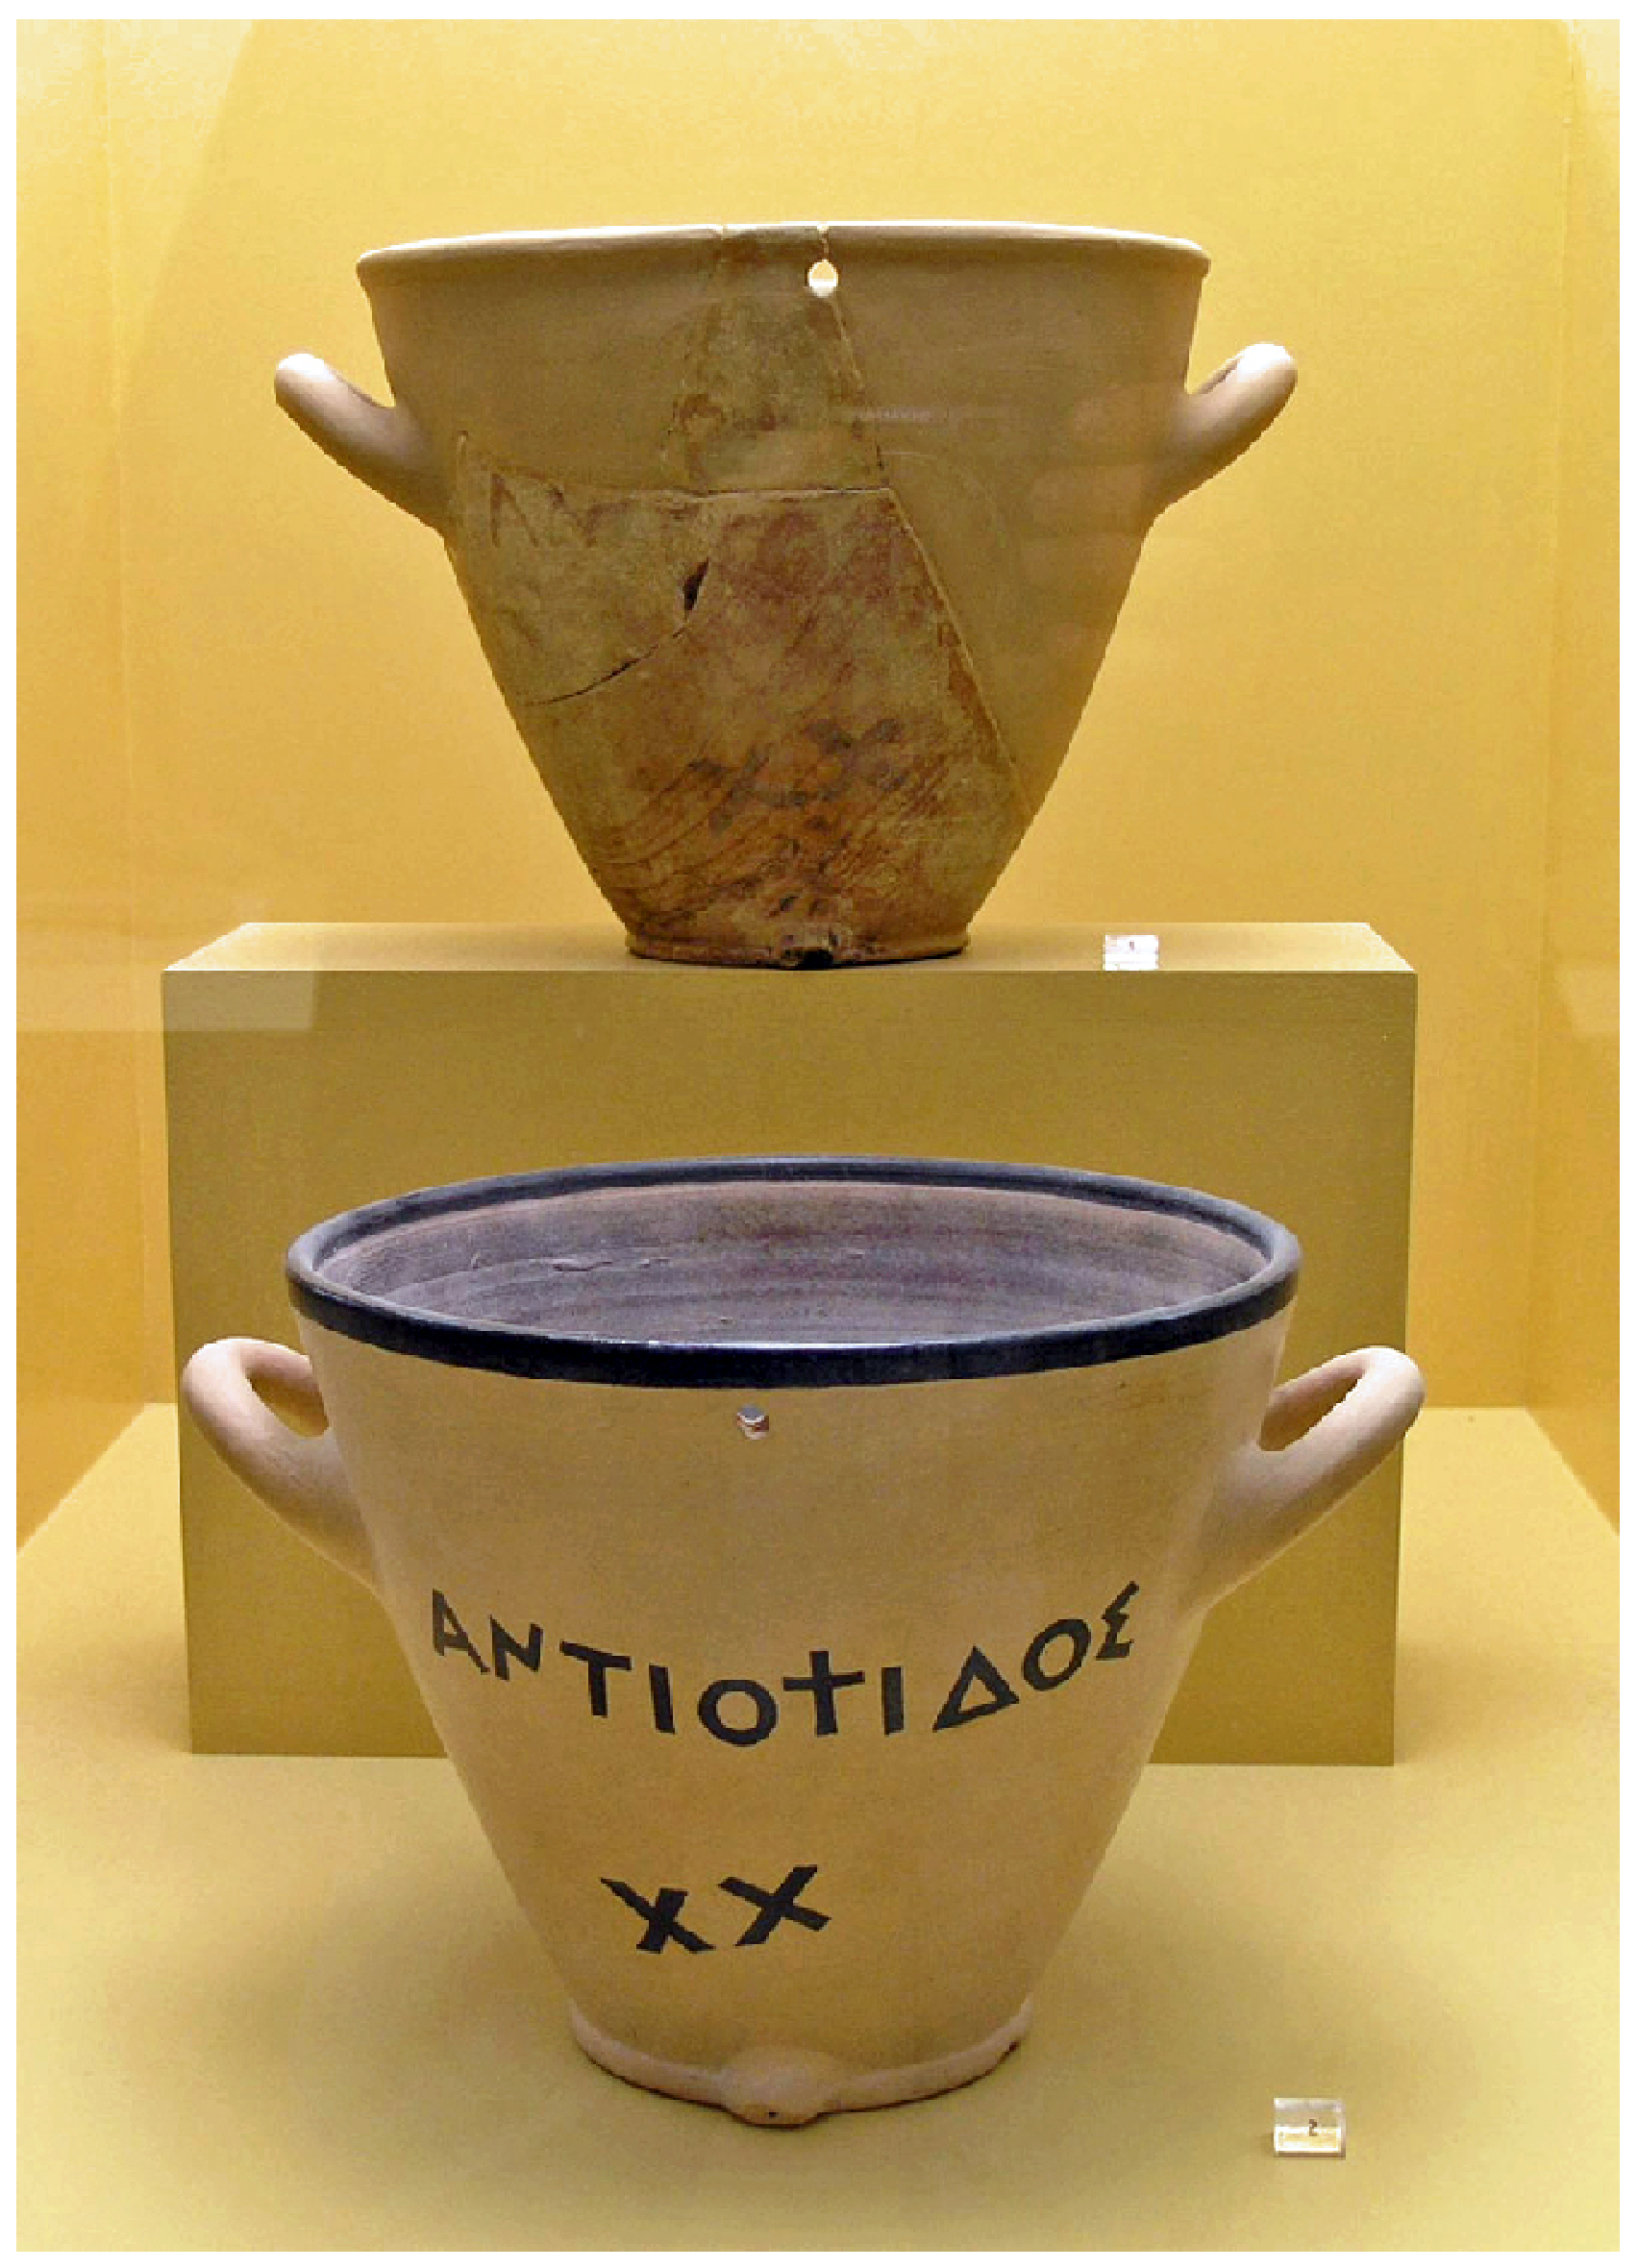
\includegraphics[width=0.45\linewidth,height=10cm]{fig/AGMA_Clepsydre_m.eps}
        \label{fig-clep}
        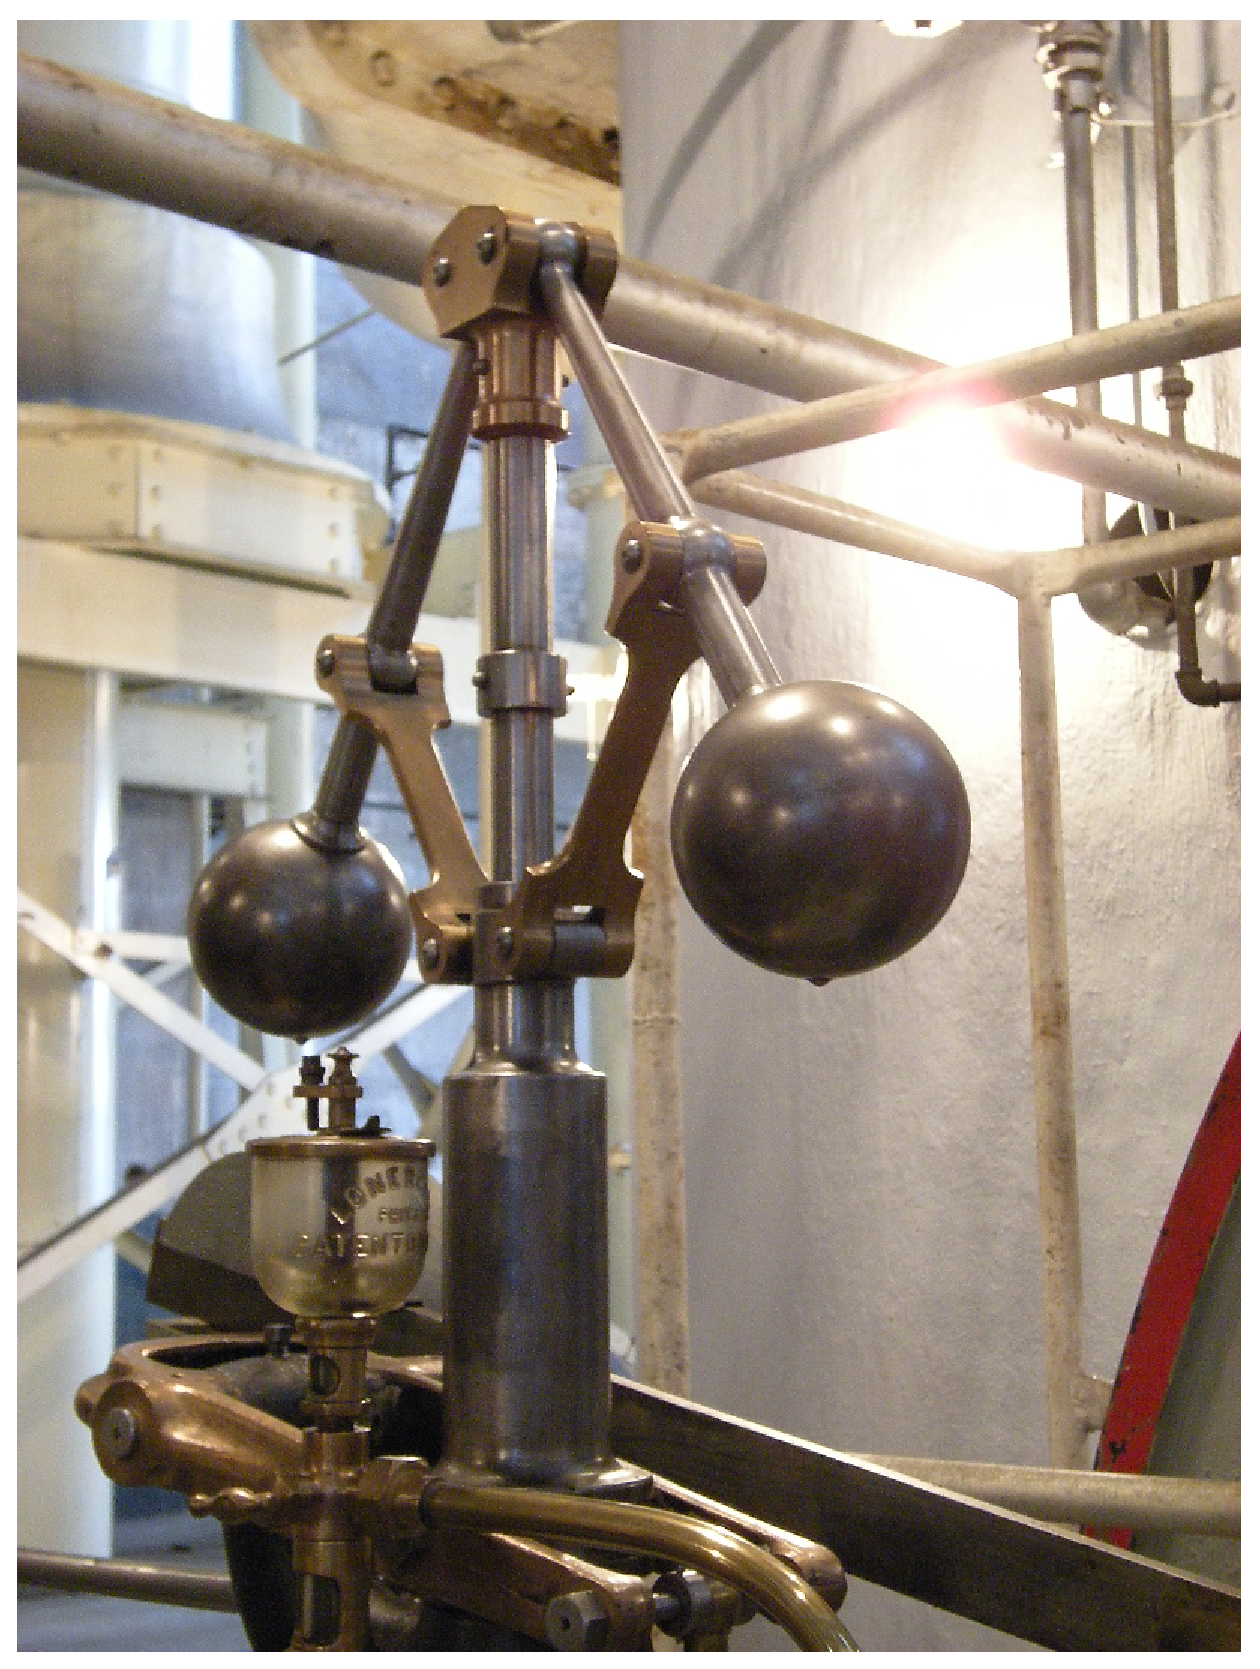
\includegraphics[width=0.45\linewidth,height=10cm]{fig/Georgetown_PowerPlant_Museum_m.eps}
        \label{fig-watt}
    \caption{Exemples historiques de régulateurs.\label{fig-hist}}
\end{figure}

%%%%%%%%%%%%%%%%%%%%%%%%%%%%%%%%%%%%%%%%%%%%%%%%%%%%%%%%%%%%%%%%%%%%%%
%%%%%%%%%%%%%%%%%%%%%%%%%%%%%%%%%%%%%%%%%%%%%%%%%%%%%%%%%%%%%%%%%%%%%%
%%%%%%%%%%%%%%%%%%%%%%%%%%%%%%%%%%%%%%%%%%%%%%%%%%%%%%%%%%%%%%%%%%%%%%
\section{Organisation d'un asservissement}
%%%%%%%%%%%%%%%%%%%%%%%%%%%%%%%%%%%%%%%%%%%%%%%%%%%%%%%%%%%%%%%%%%%%%%
%%%%%%%%%%%%%%%%%%%%%%%%%%%%%%%%%%%%%%%%%%%%%%%%%%%%%%%%%%%%%%%%%%%%%%
%%%%%%%%%%%%%%%%%%%%%%%%%%%%%%%%%%%%%%%%%%%%%%%%%%%%%%%%%%%%%%%%%%%%%%

%%%%%%%%%%%%%%%%%%%%%%%%%%%%%%%%%%%%%%%%%%%%%%%%%%%%%%%%%%%%%%%%%%%%%%
%   Nom des noeuds
%                                      
%   E ---- a ---- b ---- c ---- S
%          |                |
%          |                |
%            ---- d ------- 
% E : entrée
% a : comparateur
% b : correcteur
% c : système
% S : sortie
% d : capteur
% r : noeud décalé pour le retour
%%%%%%%%%%%%%%%%%%%%%%%%%%%%%%%%%%%%%%%%%%%%%%%%%%%%%%%%%%%%%%%%%%%%%%
\begin{center}
    \begin{tikzpicture}
        \sbEntree{E}
        \sbComp{a}{E}
        \sbRelier[$E(p)$]{E}{a}           % entree
        \sbBloc[3]{b}{$C(p)$}{a}
        \sbRelier[$\epsilon(p)$]{a}{b}    % ecart
        \sbBloc[3]{c}{$H(p)$}{b}
        \sbRelier[$U(p)$]{b}{c}           % commande
        \sbSortie[4]{S}{c}
        \sbRelier{c}{S}
        \sbNomLien[0.8]{S}{$S(p)$}
        \sbDecaleNoeudy[6]{b-c}{r}
        \sbBlocr[-1.6]{d}{$G(p)$}{r}
        \sbRelieryx{c-S}{d}              
        \sbRelierxy[$M(p)$]{d}{a}         % mesure (image de S)
        \node[yshift=-0.8em] at (b.south) {\small Correcteur};
        \node[yshift=-0.8em] at (c.south) {\small Système};
        \node[yshift=-0.8em] at (d.south) {\small Capteur};
        \node[yshift=-0.8em,xshift=0.5em] at (E.south) {\small Consigne};
        \node[yshift=-0.8em] at (S.south) {\small Sortie};
    \end{tikzpicture}
\end{center}

\begin{center}
    \begin{tikzpicture}
        \sbEntree{E}
        \sbComp{a}{E}
        \sbRelier[$E(p)$]{E}{a}           % entree
        \sbBloc[3]{b}{$C(p)$}{a}
        \sbRelier[$\epsilon(p)$]{a}{b}    % ecart
        \sbBloc[4.2]{c}{$H(p)$}{b}
        \sbRelier[$U(p)$]{b}{c}           % commande
        \sbSortie[4]{S}{c}
        \sbRelier{c}{S}
        \sbNomLien[0.8]{S}{$S(p)$}
        \sbDecaleNoeudy[7]{b-c}{r}
        \sbBlocr[-1.6]{d}{$G(p)$}{r}
        \sbRelieryx{c-S}{d}              
        \sbRelierxy[$M(p)$]{d}{a}         % mesure (image de S)
        \node[yshift=-0.8em] at (b.south) {\small Correcteur};
        \node[yshift=-0.8em] at (c.south) {\small Système};
        \node[yshift=-0.8em] at (d.south) {\small Capteur};
        \draw[dashed,very thick,blue] (1.15,-1.8) rectangle node[blue,xshift=-1.999999999em,yshift=4em] {\textbf{Régulateur}} (4.9,1);
    \end{tikzpicture}
\end{center}

%%%%%%%%%%%%%%%%%%%%%%%%%%%%%%%%%%%%%%%%%%%%%%%%%%%%%%%%%%%%%%%%%%%%%%
%   Nom des noeuds
%                                      
%                                      
%   E ---- a ---- b ---- c ---- d ---- e ---- S
%                 |                       |
%                 |                       |
%                  --------- f -----------
% E : entrée
% a : adaptateur 
% b : comparateur
% c : correcteur
% d : actionneur
% e : système
% S : sortie
% f : capteur
% r : noeud décalé pour le retour
%%%%%%%%%%%%%%%%%%%%%%%%%%%%%%%%%%%%%%%%%%%%%%%%%%%%%%%%%%%%%%%%%%%%%%
\begin{center}
    \begin{tikzpicture}
        \sbEntree{E}
        \sbBloc[3]{a}{$A_d(p)$}{E}
        \sbRelier[$E(p)$]{E}{a}
        \sbComp{b}{a}
        \sbRelier{a}{b}
        \sbBloc[3]{c}{$C(p)$}{b}
        \sbRelier[$\epsilon(p)$]{b}{c}
        \sbBloc[3]{d}{$A_c(p)$}{c}
        \sbRelier[$\epsilon'(p)$]{c}{d}
        \sbBloc[3]{e}{$H(p)$}{d}
        \sbRelier[$U(p)$]{d}{e}
        \sbSortie[4]{S}{e}
        \sbRelier{e}{S}
        \sbDecaleNoeudy[5]{d}{r}
        \sbBlocr[-1.6]{f}{$G(p)$}{r}
        \sbRelieryx{e-S}{f}              
        \sbRelierxy[$M(p)$]{f}{b}        % Mesure
        \sbNomLien[0.8]{S}{$S(p)$}
    \end{tikzpicture}
\end{center}

%%%%%%%%%%%%%%%%%%%%%%%%%%%%%%%%%%%%%%%%%%%%%%%%%%%%%%%%%%%%%%%%%%%%%%
%   Nom des noeuds
%                                      P
%                                      |
%                                      |
%   E ---- a ---- b ---- c ---- d ---- e ---- f ---- S
%                 |                              |
%                 |                              |
%                  ------------ g ---------------
% E : entrée
% a : adaptateur 
% b : comparateur
% c : correcteur
% d : actionneur
% e : sommateur (perturbation)
% P : perturbation
% f : système 
% S : sortie
% g : capteur
% r : noeud décalé pour le retour
%%%%%%%%%%%%%%%%%%%%%%%%%%%%%%%%%%%%%%%%%%%%%%%%%%%%%%%%%%%%%%%%%%%%%%
\begin{landscape}
\vspace*{\fill}
\begin{center}
    \begin{tikzpicture}
        \sbEntree{E}
        \sbBloc[3]{a}{$A_d(p)$}{E}
        \sbRelier[$E(p)$]{E}{a}
        \sbComp{b}{a}
        \sbRelier{a}{b}
        \sbBloc[3]{c}{$C(p)$}{b}
        \sbRelier[$\epsilon(p)$]{b}{c}
        \sbBloc[3]{d}{$A_c(p)$}{c}
%        \sbRelier[$\epsilon'(p)$]{c}{d}
        \sbRelier{c}{d}
        \sbSumh[6.7]{e}{d}
        \sbDecaleNoeudy[-3]{e}{P}
        \sbRenvoiF[-3]{P}{e}{$P(p)$}
        \sbRelier[$U(p)$]{d}{e}
        \sbBloc{f}{$H(p)$}{e}
        \sbRelier{e}{f}
        \sbSortie[4]{S}{f}
        \sbRelier{f}{S}
        \sbDecaleNoeudy[5]{c}{r}
        \sbBlocr[-1.6]{g}{$G(p)$}{r}
        \sbRelieryx{f-S}{g}              
        \sbRelierxy[$M(p)$]{g}{b}        
        \sbNomLien[0.8]{S}{$S(p)$}
        \node[yshift=-0.8em] at (a.south) {\small Adaptateur};
        \node[yshift=-0.8em] at (c.south) {\small Correcteur};
        \node[yshift=-0.8em] at (d.south) {\small Actionneur};
        \node[yshift=-0.8em] at (f.south) {\small Système};
        \node[yshift=-0.8em] at (g.south) {\small Capteur};
        \node[yshift=-0.8em,xshift=0.5em] at (E.south) {\small Consigne};
        \node[yshift=-0.8em] at (S.south) {\small Sortie};
        \node[yshift=2em,xshift=2.8em] at (P.east) {\small Perturbation};
        \draw[dashed,very thick,blue](-0.8,-4) 
         rectangle node[blue,xshift=-3.2em,yshift=7em]{\textbf{Chaîne d'information}}(6.9,2.5);
        \draw[dashed,very thick,red](7.3,-4)
         rectangle node[red,xshift=-5.9em,yshift=7em]  {\textbf{Chaîne d'énergie}    }(15.9,2.5);
         \draw[very thick,green!50!black,dashed,-latex] (4,1)   -- node[green!50!black,above] {Chaîne direct} (14,1) ;
         \draw[very thick,green!50!black,dashed,-latex] (14,-3.7) -- node[green!50!black,above] {Chaîne de retour} (4,-3.7) ;
    \end{tikzpicture}
\end{center}
    \captionof{figure}{Décomposition en chaîne d'information et chaîne 
                       d'énergie d'un schéma bloc d'asservissement complet}
\vspace*{\fill}
\end{landscape}

\begin{center}
    \begin{tabular}{M{3cm}M{8cm}M{4cm}N}
        \hhline{===}
        Composants      & Description & Fonction de transfert ou signal associés &\\[2em]
        \hhline{===}
        Consigne/Entrée & La valeur que l'on souhaite atteindre en sortie du système asservi.
                          Cette consigne peut être constante ou dépendante du temps. 
                        & $E(p)$                                                 &\\[5em]
        \hline
        Adaptateur      & Adapte le signal de consigne à l'image de la sortie.           
                        & $A_d(p)$                                               &\\[3em]
        \hline
        Correcteur      & \'Elabore à partir du signal d'écart $\epsilon(p)$ 
                          la commande $U(p)$ ou la grandeur réglante du système.
                        & $C(p)$                                                 & \\[3em]
        \hline
        Actionneur      & L'organe d'action qui apporte l'énergie au système.
                        & $A_c(p)$                                               &\\[3em]
        \hline
        Système         & Le système que l'on souhaite contrôler et/ou asservir
                                      & $H(p)$                                   &\\[3em]
        \hline
        Régulateur      & Le régulateur se compose d'un comparateur qui élabore le signal d'écart $\epsilon(p)$ 
                          à partir de la consigne et de la mesure, formellement le régulateur incorpore le correcteur 
                          et du correcteur.
                                      & $\epsilon(p)$                            &\\[3em]
        \hline
        Perturbation    & Phénomène physique intervenant sur le système qui en modifie la sortie
                                      & $P(p)$                                   &\\[3em]
        \hline
        Capteur         &  Le capteur prélève le sortie pour en donner une image (la mesure) 
                           utile au régulateur. Intervenant dans la boucle ouverte, son étude 
                           est indispensable pour la caractérisation des performances du système asservi.
                                      & $G(p)$                                   &\\[3em]
        \hline
        Sortie          & Le signal de sortie du système que l'on souhaite régulé et/ou asservir
                                      & $S(p)$                                   &\\[3em]
        \hhline{===}
    \end{tabular}
\end{center}


%%%%%%%%%%%%%%%%%%%%%%%%%%%%%%%%%%%%%%%%%%%%%%%%%%%%%%%%%%%%%%%%%%%%%%
%%%%%%%%%%%%%%%%%%%%%%%%%%%%%%%%%%%%%%%%%%%%%%%%%%%%%%%%%%%%%%%%%%%%%%
%%%%%%%%%%%%%%%%%%%%%%%%%%%%%%%%%%%%%%%%%%%%%%%%%%%%%%%%%%%%%%%%%%%%%%
\section{Performances des systèmes asservis}
%%%%%%%%%%%%%%%%%%%%%%%%%%%%%%%%%%%%%%%%%%%%%%%%%%%%%%%%%%%%%%%%%%%%%%
%%%%%%%%%%%%%%%%%%%%%%%%%%%%%%%%%%%%%%%%%%%%%%%%%%%%%%%%%%%%%%%%%%%%%%
%%%%%%%%%%%%%%%%%%%%%%%%%%%%%%%%%%%%%%%%%%%%%%%%%%%%%%%%%%%%%%%%%%%%%%

\subsection{Précision}

\subsection{Rapidité}

\subsection{Dépassement}


%%%%%%%%%%%%%%%%%%%%%%%%%%%%%%%%%%%%%%%%%%%%%%%%%%%%%%%%%%%%%%%%%%%%%%
%%%%%%%%%%%%%%%%%%%%%%%%%%%%%%%%%%%%%%%%%%%%%%%%%%%%%%%%%%%%%%%%%%%%%%
%%%%%%%%%%%%%%%%%%%%%%%%%%%%%%%%%%%%%%%%%%%%%%%%%%%%%%%%%%%%%%%%%%%%%%
\section{Asservissement d'un système du premier ordre}
%%%%%%%%%%%%%%%%%%%%%%%%%%%%%%%%%%%%%%%%%%%%%%%%%%%%%%%%%%%%%%%%%%%%%%
%%%%%%%%%%%%%%%%%%%%%%%%%%%%%%%%%%%%%%%%%%%%%%%%%%%%%%%%%%%%%%%%%%%%%%
%%%%%%%%%%%%%%%%%%%%%%%%%%%%%%%%%%%%%%%%%%%%%%%%%%%%%%%%%%%%%%%%%%%%%%

\begin{center}
    \begin{tikzpicture}
        \sbEntree{E}
        \sbComp{a}{E}
        \sbRelier[$E(p)$]{E}{a}
       % \sbBloc{b}{$C(p)$}{a}
        \sbBloc{b}{$H(p)$}{a}
        \sbRelier{a}{b}
        \sbSortie[4]{S}{b}
        \sbRelier{b}{S}
        \sbRenvoi{b-S}{a}{}
        \sbNomLien[0.8]{S}{$S(p)$}
    \end{tikzpicture}
\end{center}



%%%%%%%%%%%%%%%%%%%%%%%%%%%%%%%%%%%%%%%%%%%%%%%%%%%%%%%%%%%%%%%%%%%%%%
%%%%%%%%%%%%%%%%%%%%%%%%%%%%%%%%%%%%%%%%%%%%%%%%%%%%%%%%%%%%%%%%%%%%%%
%%%%%%%%%%%%%%%%%%%%%%%%%%%%%%%%%%%%%%%%%%%%%%%%%%%%%%%%%%%%%%%%%%%%%%
\section{Asservissement d'un système du second ordre}
%%%%%%%%%%%%%%%%%%%%%%%%%%%%%%%%%%%%%%%%%%%%%%%%%%%%%%%%%%%%%%%%%%%%%%
%%%%%%%%%%%%%%%%%%%%%%%%%%%%%%%%%%%%%%%%%%%%%%%%%%%%%%%%%%%%%%%%%%%%%%
%%%%%%%%%%%%%%%%%%%%%%%%%%%%%%%%%%%%%%%%%%%%%%%%%%%%%%%%%%%%%%%%%%%%%%

\begin{center}
    \begin{tikzpicture}
        \sbEntree{E}
        \sbComp{a}{E}
        \sbRelier[$E(p)$]{E}{a}
       % \sbBloc{b}{$C(p)$}{a}
        \sbBloc{b}{$H(p)$}{a}
        \sbRelier{a}{b}
        \sbSortie[4]{S}{b}
        \sbRelier{b}{S}
        \sbRenvoi{b-S}{a}{}
        \sbNomLien[0.8]{S}{$S(p)$}
    \end{tikzpicture}
\end{center}
\newpage
%%%%%%%%%%%%%%%%%%%%%%%%%%%%%%%%%%%%%%%%%%%%%%%%%%%%%%%%%%%%%%%%%%%%%%
%%%%%%%%%%%%%%%%%%%%%%%%%%%%%%%%%%%%%%%%%%%%%%%%%%%%%%%%%%%%%%%%%%%%%%
%%%%%%%%%%%%%%%%%%%%%%%%%%%%%%%%%%%%%%%%%%%%%%%%%%%%%%%%%%%%%%%%%%%%%%
\section*{Exercices du chapitre}
%%%%%%%%%%%%%%%%%%%%%%%%%%%%%%%%%%%%%%%%%%%%%%%%%%%%%%%%%%%%%%%%%%%%%%
%%%%%%%%%%%%%%%%%%%%%%%%%%%%%%%%%%%%%%%%%%%%%%%%%%%%%%%%%%%%%%%%%%%%%%
%%%%%%%%%%%%%%%%%%%%%%%%%%%%%%%%%%%%%%%%%%%%%%%%%%%%%%%%%%%%%%%%%%%%%%


\exercice{}
\question

\newpage
%%%%%%%%%%%%%%%%%%%%%%%%%%%%%%%%%%%%%%%%%%%%%%%%%%%%%%%%%%%%%%%%%%%%%%
%%%%%%%%%%%%%%%%%%%%%%%%%%%%%%%%%%%%%%%%%%%%%%%%%%%%%%%%%%%%%%%%%%%%%%
%%%%%%%%%%%%%%%%%%%%%%%%%%%%%%%%%%%%%%%%%%%%%%%%%%%%%%%%%%%%%%%%%%%%%%
\section*{Corrigé des exercices}
%%%%%%%%%%%%%%%%%%%%%%%%%%%%%%%%%%%%%%%%%%%%%%%%%%%%%%%%%%%%%%%%%%%%%%
%%%%%%%%%%%%%%%%%%%%%%%%%%%%%%%%%%%%%%%%%%%%%%%%%%%%%%%%%%%%%%%%%%%%%%
%%%%%%%%%%%%%%%%%%%%%%%%%%%%%%%%%%%%%%%%%%%%%%%%%%%%%%%%%%%%%%%%%%%%%%


 
{\tikzset{external/export=false}
\chapter{Précision des systèmes asservis\label{chap-perf}}



\newpage
%%%%%%%%%%%%%%%%%%%%%%%%%%%%%%%%%%%%%%%%%%%%%%%%%%%%%%%%%%%%%%%%%%%%%%
%%%%%%%%%%%%%%%%%%%%%%%%%%%%%%%%%%%%%%%%%%%%%%%%%%%%%%%%%%%%%%%%%%%%%%
%%%%%%%%%%%%%%%%%%%%%%%%%%%%%%%%%%%%%%%%%%%%%%%%%%%%%%%%%%%%%%%%%%%%%%
\section*{Exercices du chapitre}
%%%%%%%%%%%%%%%%%%%%%%%%%%%%%%%%%%%%%%%%%%%%%%%%%%%%%%%%%%%%%%%%%%%%%%
%%%%%%%%%%%%%%%%%%%%%%%%%%%%%%%%%%%%%%%%%%%%%%%%%%%%%%%%%%%%%%%%%%%%%%
%%%%%%%%%%%%%%%%%%%%%%%%%%%%%%%%%%%%%%%%%%%%%%%%%%%%%%%%%%%%%%%%%%%%%%


\exercice{}
\question

\newpage
%%%%%%%%%%%%%%%%%%%%%%%%%%%%%%%%%%%%%%%%%%%%%%%%%%%%%%%%%%%%%%%%%%%%%%
%%%%%%%%%%%%%%%%%%%%%%%%%%%%%%%%%%%%%%%%%%%%%%%%%%%%%%%%%%%%%%%%%%%%%%
%%%%%%%%%%%%%%%%%%%%%%%%%%%%%%%%%%%%%%%%%%%%%%%%%%%%%%%%%%%%%%%%%%%%%%
\section*{Corrigé des exercices}
%%%%%%%%%%%%%%%%%%%%%%%%%%%%%%%%%%%%%%%%%%%%%%%%%%%%%%%%%%%%%%%%%%%%%%
%%%%%%%%%%%%%%%%%%%%%%%%%%%%%%%%%%%%%%%%%%%%%%%%%%%%%%%%%%%%%%%%%%%%%%
%%%%%%%%%%%%%%%%%%%%%%%%%%%%%%%%%%%%%%%%%%%%%%%%%%%%%%%%%%%%%%%%%%%%%%


 
%%%%%%%%%%%%%%%%%%%%%%%%%%%%%%%%%%%%%%%%%%%%%%%%%%%%%%%%%%%%%%%%%%%%%%
%%%%%%%%%%%%%%%%%%%%%%%%%%%%%%%%%%%%%%%%%%%%%%%%%%%%%%%%%%%%%%%%%%%%%%
%%%%%%%%%%%%%%%%%%%%%%%%%%%%%%%%%%%%%%%%%%%%%%%%%%%%%%%%%%%%%%%%%%%%%%
%%%%%%%%%%%%%%%%%%%%%%%%%%%%%%%%%%%%%%%%%%%%%%%%%%%%%%%%%%%%%%%%%%%%%%
\chapter{Stabilité des systèmes asservis\label{chap-stab}}
%%%%%%%%%%%%%%%%%%%%%%%%%%%%%%%%%%%%%%%%%%%%%%%%%%%%%%%%%%%%%%%%%%%%%%
%%%%%%%%%%%%%%%%%%%%%%%%%%%%%%%%%%%%%%%%%%%%%%%%%%%%%%%%%%%%%%%%%%%%%%
%%%%%%%%%%%%%%%%%%%%%%%%%%%%%%%%%%%%%%%%%%%%%%%%%%%%%%%%%%%%%%%%%%%%%%
%%%%%%%%%%%%%%%%%%%%%%%%%%%%%%%%%%%%%%%%%%%%%%%%%%%%%%%%%%%%%%%%%%%%%%
\minitoc
\newpage

%%%%%%%%%%%%%%%%%%%%%%%%%%%%%%%%%%%%%%%%%%%%%%%%%%%%%%%%%%%%%%%%%%%%%%
%%%%%%%%%%%%%%%%%%%%%%%%%%%%%%%%%%%%%%%%%%%%%%%%%%%%%%%%%%%%%%%%%%%%%%
%%%%%%%%%%%%%%%%%%%%%%%%%%%%%%%%%%%%%%%%%%%%%%%%%%%%%%%%%%%%%%%%%%%%%%
\section{Définitions de la stabilité}
%%%%%%%%%%%%%%%%%%%%%%%%%%%%%%%%%%%%%%%%%%%%%%%%%%%%%%%%%%%%%%%%%%%%%%
%%%%%%%%%%%%%%%%%%%%%%%%%%%%%%%%%%%%%%%%%%%%%%%%%%%%%%%%%%%%%%%%%%%%%%
%%%%%%%%%%%%%%%%%%%%%%%%%%%%%%%%%%%%%%%%%%%%%%%%%%%%%%%%%%%%%%%%%%%%%%

\textbf{Un système est dit stable si à une entrée bornée le système produit une sortie bornée}\footnote{Chez 
nos amis anglo-saxons, on rencontre le concept de BIBO (\og bounded input bounded output\fg)}

\textbf{Un système est dit stable lorsque écarté de sa position d'équilibre, il tend à y revenir}

Ces deux définitions sont équivalentes dans le cas des \glspl{slci}. 

\begin{figure}[!h]
    \centering
\tikzsetnextfilename{stable_1-chap6_ext}
    \begin{tikzpicture}
        \draw[green!50!black,line width=0.5mm] (0,0.25) circle (1.5ex);
        \draw[thick] (0,0) parabola (1,1.75) ;
        \draw[thick] (0,0) parabola (-1,1.75) ;
        \node at (0,-2.5) {(a) stable};
        \begin{scope}[xshift=3.5cm]
            \draw[red,line width=0.5mm] (0,0.25) circle (1.5ex);
            \draw[thick] (0,0) parabola (1,-1.75) ;
            \draw[thick] (0,0) parabola (-1,-1.75) ;
            \node at (0,-2.5) {(b) instable};
        \end{scope}
        \begin{scope}[xshift=7cm]
            \draw[blue,line width=0.5mm] (0,0.25) circle (1.5ex);
            \draw[thick] (0,0) parabola (-1,1.75) ;
            \draw[thick] (0,0) parabola (0.5,0.2) ;
            \draw[thick] (0.5,0.2) parabola (1,-1.75) ;
            \node[text width=3cm,align=center] at (0,-2.5) {(c) stabilité\\conditionnelle};
        \end{scope}
    \end{tikzpicture}
\caption{Représentation schématique de la stabilité}
\end{figure}


\begin{center}
\tikzsetnextfilename{stable-chap0_ext}
\begin{tikzpicture}
	\begin{axis}
	[	ticks=none,
        axis line style = thick,
        height=5cm,
        width=5cm,
        axis x line=center,
        axis y line=center,
        xmin=-2,
        xmax=10,
        ymin=-1.5,
        ymax=3.0,
        xlabel={$t$},
        ylabel={$s(t)$},
        xlabel style={below right},
        ylabel style={above left},
	]
	\addplot[signalb,domain=-2:0] {0};
	\addplot[signalb,domain=0:10] {sin(3*deg(x))*exp(-x)+1};
	\draw[dotted,very thick,col1] (axis cs:0,0) -- (axis cs:0,1);
	\end{axis}
\end{tikzpicture}

\end{center}                

\begin{center}
\tikzsetnextfilename{stable2-chap0_ext}
    \begin{tikzpicture}
        \begin{axis}[
	ticks=none,
        axis line style = thick,
        height=5cm,
        width=5cm,
        axis x line=center,
        axis y line=center,
        xmin=-2,
        xmax=10,
        ymin=-1.5,
        ymax=3.0,
        xlabel={$t$},
        ylabel={$s(t)$},
        xlabel style={below right},
        ylabel style={above left},
        ]                                                                                                                     
        \addplot [very thick,color=blue,domain=-2:0, samples=101]{0};
	\addplot [very thick,color=blue,domain=0:10, samples=501]{0.7*sin(3*deg(x))+1};
	\draw[dotted,very thick,blue] (axis cs:0,0) -- (axis cs:0,1);
        \end{axis}
    \end{tikzpicture}

\end{center}

\begin{center}
\tikzsetnextfilename{instable-chap0_ext}
    \begin{tikzpicture}
        \begin{axis}[
	ticks=none,
        axis line style = thick,
        height=5cm,
        width=5cm,
        axis x line=center,
        axis y line=center,
        xmin=-2,
        xmax=10,
        ymin=-3,
        ymax=6.0,
        xlabel={$t$},
        ylabel={$s(t)$},
        xlabel style={below right},
        ylabel style={above left},
        ]
        \addplot [very thick,color=red,domain=-2:0, samples=101,unbounded coords=jump]{0};
	\addplot [very thick,color=red,domain=0:10, samples=501,unbounded coords=jump]{0.8*sin(3*deg(x))*exp(0.2*x)+1};
	\draw[dotted,very thick,red] (axis cs:0,0) -- (axis cs:0,1);
        \end{axis}
    \end{tikzpicture}

\end{center}
%%%%%%%%%%%%%%%%%%%%%%%%%%%%%%%%%%%%%%%%%%%%%%%%%%%%%%%%%%%%%%%%%%%%%%
%%%%%%%%%%%%%%%%%%%%%%%%%%%%%%%%%%%%%%%%%%%%%%%%%%%%%%%%%%%%%%%%%%%%%%
%%%%%%%%%%%%%%%%%%%%%%%%%%%%%%%%%%%%%%%%%%%%%%%%%%%%%%%%%%%%%%%%%%%%%%
\section{Critère de stabilité}
%%%%%%%%%%%%%%%%%%%%%%%%%%%%%%%%%%%%%%%%%%%%%%%%%%%%%%%%%%%%%%%%%%%%%%
%%%%%%%%%%%%%%%%%%%%%%%%%%%%%%%%%%%%%%%%%%%%%%%%%%%%%%%%%%%%%%%%%%%%%%
%%%%%%%%%%%%%%%%%%%%%%%%%%%%%%%%%%%%%%%%%%%%%%%%%%%%%%%%%%%%%%%%%%%%%%

\acpl
Réponse temporelle du premier ordre du second ordre ...

\begin{criteria}{Condition fondamentale de stabilité}
    \textbf{Un système est stable si sa fonction de transfert ne possède aucun pôles à partie réelle positive.}
\end{criteria}

\tikzsetnextfilename{stabilite_plan-complexe-chap6_ext}
\clearpage
\thispagestyle{empty}
\begin{landscape}
    \centering
    %\vspace*{\fill}
    \captionsetup{width=1.15\linewidth}
    \begin{figure}[!h]
        \centering
        \begin{tikzpicture}
        \begin{axis}[                                                                                                                     ticks=none,
            width=1.6\textheight,           
            height=\textwidth,    
            axis x line=center,                                                                            
            axis y line=center,
            xmin=-12.5,                                                                                                  
            xmax=12.5,
            ymin=-5,                                                                                                         
            ymax=5,
            xlabel={\LARGE $\Re{(p)}$},
            ylabel={\LARGE $\Im{(p)}$},
            xlabel style={right},
            ylabel style={above},                                                                                       
            ]      
            \draw [white!90!blue,fill=white!95!blue]   (axis cs:-12.5,-5) rectangle (axis cs:0,5);
            \draw [white!90!black,fill=white!90!black] (axis cs:0,-5) rectangle (axis cs:12.5,5);

            \draw [ultra thick,-latex]   (axis cs:-12.5,0) -- (axis cs:12.5,0);
            \draw [ultra thick,-latex]   (axis cs:0,-5) -- (axis cs:0,5);

            \coordinate (pt01) at (axis cs:-6.5,4.5);
            \coordinate (pt02) at (axis cs:6.5,4.5);

            \coordinate (pt1) at (axis cs:-12.5,2.0);
            \addplot[mark=x,black!60!green,ultra thick,only marks,mark size=7pt]  coordinates{ (-11,1.5) (-11,-1.5) } ;      
            \draw[ultra thick,dotted,color=black!60!green] (axis cs:-11,1.5) -- (axis cs:-11,-1.5) ;

            \coordinate (pt2) at (axis cs:-7,1.0);
            \addplot[mark=x,black!10!green,ultra thick,only marks,mark size=7pt]  coordinates{ (-5,0.5) (-5,-0.5) } ;  
            \draw[ultra thick,dotted,color=black!10!green] (axis cs:-5,0.5) -- (axis cs:-5,-0.5) ;

            \coordinate (pt3) at (axis cs:-10.25,-3.0);
            \addplot[mark=x,black!50!red,ultra thick,only marks,mark size=7pt]    coordinates{ (-8,0) } ;             

            \coordinate (pt4) at (axis cs:-4.75,-3.0);
            \addplot[mark=x,red,ultra thick,only marks,mark size=7pt]    coordinates{ (-2,0) } ;                      

            \coordinate (pt5) at  (axis cs:1.25,-5);
            \coordinate (pt52) at (axis cs:1.25,-3);
            \addplot[mark=x,black,ultra thick,only marks,mark size=7pt]  coordinates{ (0,0) } ;                      

            \coordinate (pt6) at (axis cs:1.25,2);
            \coordinate (pt62) at (axis cs:1.25,0);
            \addplot[mark=x,black!50!white,ultra thick,only marks,mark size=7pt]  coordinates{ (0,2) (0,-2) } ;              
            \draw[ultra thick,dotted,color=black!50!white] (axis cs:0,-2) to[bend right] (axis cs:0,2);

            \coordinate (pt7) at (axis cs:8.25,2);
            \addplot[mark=x,blue,ultra thick,only marks,mark size=7pt]   coordinates{ (11,1.5) (11,-1.5) } ;                
            \draw[ultra thick,dotted,color=blue] (axis cs:11,1.5) -- (axis cs:11,-1.5) ;

            \coordinate (pt8) at (axis cs:6.5,-3);
            \addplot[mark=x,orange,ultra thick,only marks,mark size=7pt] coordinates{ (8,0) } ;                  

        \end{axis}


            \node at (pt01) {\textbf{\Large STABLE}};
            \node at (pt02) {\textbf{\Large INSTABLE}};
            % pt1
            \node[anchor=south west] at (pt1) {
                \begin{tikzpicture}
                    \begin{axis}[
                    ticks=none,
                    width=4cm,    
                    height=4cm,    
                    axis x line=center,                                                                            
                    axis y line=center,
                    xmin=-0.5,                                                                                                                    xmax=6.5,
                    ymin=-0.5,                                                                        
                    ymax=2.5,
                    xlabel={$t$},
                    ylabel={$s(t)$},
                    xlabel style={below right},
                    ylabel style={right}
                    ]
                    \addplot [very thick,color=black!60!green,domain=0:10, samples=501,unbounded coords=jump]{1.2*sin(4.5*deg(x))*exp(-0.7*x)};
                    \addplot [thick,dotted,color=black,domain=0:10, samples=501,unbounded coords=jump]{1.2*exp(-0.7*x)+1};
                    \addplot [thick,dotted,color=black,domain=0:10, samples=501,unbounded coords=jump]{-1.2*exp(-0.7*x)+1};
                    \end{axis}
                \end{tikzpicture}
            };

            % pt2
            \node[anchor=south west] at (pt2) {
                \begin{tikzpicture}
                    \begin{axis}[
                    ticks=none,
                    width=4cm,    
                    height=4cm,    
                    axis x line=center,                                                                            
                    axis y line=center,
                    xmin=-0.5,                                                                                                                    xmax=6.5,
                    ymin=-0.5,                                                                        
                    ymax=2.5,
                    xlabel={$t$},
                    ylabel={$s(t)$},
                    xlabel style={below right},
                    ylabel style={right}
                    ]
                    \addplot [very thick,color=black!10!green,domain=0:10, samples=501,unbounded coords=jump]{1.2*sin(2.5*deg(x))*exp(-0.5*x)};
                    \addplot [thick,dotted,color=black,domain=0:10, samples=501,unbounded coords=jump]{1.2*exp(-0.5*x)+1};
                    \addplot [thick,dotted,color=black,domain=0:10, samples=501,unbounded coords=jump]{-1.2*exp(-0.5*x)+1};
                    \end{axis}
                \end{tikzpicture}
            };
            % pt3
            \node[anchor=south west] at (pt3) {
                \begin{tikzpicture}
                    \begin{axis}[
                    ticks=none,
                    width=4cm,    
                    height=4cm,    
                    axis x line=center,                                                                            
                    axis y line=center,
                    xmin=-0.5,                                                                                                                    xmax=6.5,
                    ymin=-0.5,                                                                        
                    ymax=3,
                        xlabel={$t$},
                        ylabel={$s(t)$},
                    xlabel style={below right},
                    ylabel style={right}
                    ]
                    \addplot [very thick,color=black!30!red,domain=0:10, samples=501,unbounded coords=jump]{2*exp(-0.75*x)};
                    \end{axis}
                \end{tikzpicture}
            };
            % pt4
            \node[anchor=south west] at (pt4) {
                \begin{tikzpicture}
                    \begin{axis}[
                    ticks=none,
                    width=4cm,    
                    height=4cm,    
                    axis x line=center,                                                                            
                    axis y line=center,
                    xmin=-0.5,                                                                                                                    xmax=6.5,
                    ymin=-0.5,                                                                        
                    ymax=3,
                        xlabel={$t$},
                        ylabel={$s(t)$},
                    xlabel style={below right},
                    ylabel style={right}
                    ]
                    \addplot [very thick,color=red,domain=0:10, samples=501,unbounded coords=jump]{2*exp(-0.25*x)};
                    \end{axis}
                \end{tikzpicture}
            };
            % pt5
            \node[anchor=south west] at (pt5) {
                \begin{tikzpicture}
                    \begin{axis}[
                    ticks=none,
                    width=4cm,    
                    height=4cm,    
                    axis x line=center,                                                                            
                    axis y line=center,
                    xmin=-0.5,                                                                                                                    xmax=6.5,
                    ymin=-0.5,                                                                        
                    ymax=3,
                    xlabel={$t$},
                    ylabel={$s(t)$},
                    xlabel style={below right},
                    ylabel style={right}
                    ]
                    \addplot [very thick,color=black,domain=0:10, samples=501,unbounded coords=jump]{1.5};
                    \end{axis}
                \end{tikzpicture}
            };
            % pt52
            \node[anchor=south west] at (pt52) {
                \begin{tikzpicture}
                    \begin{axis}[
                    ticks=none,
                    width=4cm,    
                    height=4cm,    
                    axis x line=center,                                                                            
                    axis y line=center,
                    xmin=-0.5,                                                                                                                    xmax=15,
                    ymin=-0.5,                                                                        
                    ymax=6,
                    xlabel={$t$},
                    ylabel={$s(t)$},
                    xlabel style={below right},
                    ylabel style={right}
                    ]
                    \addplot [very thick,color=black,domain=0:15, samples=501,unbounded coords=jump]{1+exp(0.1*x)};
                    \end{axis}
            \end{tikzpicture}
            };
            % pt6
            \node[anchor=south west] at (pt6) {
                \begin{tikzpicture}
                    \begin{axis}[
                    ticks=none,
                    width=4cm,    
                    height=4cm,    
                    axis x line=center,                                                                            
                    axis y line=center,
                    xmin=-0.5,                                                                                                                    xmax=8,
                    ymin=-20,                                                                        
                    ymax=20,
                    xlabel={$t$},
                    ylabel={$s(t)$},
                    xlabel style={below right},
                    ylabel style={right}
                    ]
              \addplot [very thick,color=black!50!white,domain=0:10, samples=501,unbounded coords=jump]{sin(2.5*deg(x))*exp(0.40*x)+1};
              \addplot [thick,dotted,color=black!50!white,domain=0:10, samples=501,unbounded coords=jump]{ exp(0.4*x)+1};
              \addplot [thick,dotted,color=black!50!white,domain=0:10, samples=501,unbounded coords=jump]{-exp(0.4*x)+1};
                    \end{axis}
                \end{tikzpicture}
            };
            % pt62
            \node[anchor=south west] at (pt62) {
                \begin{tikzpicture}
                    \begin{axis}[
                    ticks=none,
                    width=4cm,    
                    height=4cm,    
                    axis x line=center,                                                                            
                    axis y line=center,
                    xmin=-0.5,                                                                                                                    xmax=6.5,
                    ymin=-2.5,                                                                        
                    ymax=2.5,
                    xlabel={$t$},
                    ylabel={$s(t)$},
                    xlabel style={below right},
                    ylabel style={right}
                    ]
                    \addplot [very thick,color=black!50!white,domain=0:10, samples=501,unbounded coords=jump]{sin(2.5*deg(x))};
                    \end{axis}
                \end{tikzpicture}
            };
            % pt7
            \node[anchor=south west] at (pt7) {
                \begin{tikzpicture}
                    \begin{axis}[
                    ticks=none,
                    width=4cm,    
                    height=4cm,    
                    axis x line=center,                                                                            
                    axis y line=center,
                    xmin=-0.5,                                                                                                                    xmax=8.0,
                    ymin=-20,                                                                        
                    ymax=20,
                    xlabel={$t$},
                    ylabel={$s(t)$},
                    xlabel style={below right},
                    ylabel style={right}
                    ]
              \addplot [very thick,color=blue,domain=0:10, samples=501,unbounded coords=jump]{sin(2.5*deg(x))*exp(0.40*x)+1};
              \addplot [thick,dotted,color=black,domain=0:10, samples=501,unbounded coords=jump]{ exp(0.4*x)+1};
              \addplot [thick,dotted,color=black,domain=0:10, samples=501,unbounded coords=jump]{-exp(0.4*x)+1};
                    \end{axis}
              \end{tikzpicture}
            };
            % pt8
            \node[anchor=south west] at (pt8) {
                \begin{tikzpicture}
                    \begin{axis}[
                    ticks=none,
                    width=4cm,    
                    height=4cm,    
                    axis x line=center,                                                                            
                    axis y line=center,
                    xmin=-0.5,                                                                                                                    xmax=15,
                    ymin=-0.5,                                                                        
                    ymax=6,
                    xlabel={$t$},
                    ylabel={$s(t)$},
                    xlabel style={below right},
                    ylabel style={right}
                    ]
                    \addplot[very thick,color=orange,domain=0:15,samples=501,unbounded coords=jump]{1+exp(0.1*x)};
                    \end{axis}
                \end{tikzpicture}
            };
        \end{tikzpicture}
    \caption{Stabilité d'un SLCI d'après la carte des pôles de sa fonction de transfert et de leurs
    réponses impulsionnelles.
    (Vert) Deux pôles complexes conjugués. 
    (Rouge) Pôle à partie réel négative. 
    (Gris) Deux pôles complexes conjugués à partie réelle nulle.
    (Noir) Pôle nul.
    (Bleu) Deux pôles complexes conjugués à partie réelle positive.
    (Orange) Pôle à partie réel positive.}
    \end{figure}
%    %\vfill
\end{landscape}

\clearpage
\pagestyle{fancy}
\captionsetup{width=0.8\linewidth}


%%%%%%%%%%%%%%%%%%%%%%%%%%%%%%%%%%%%%%%%%%%%%%%%%%%%%%%%%%%%%%%%%%%%%%
\paragraph{Notion de pôles dominants}
%%%%%%%%%%%%%%%%%%%%%%%%%%%%%%%%%%%%%%%%%%%%%%%%%%%%%%%%%%%%%%%%%%%%%%

%%%%%%%%%%%%%%%%%%%%%%%%%%%%%%%%%%%%%%%%%%%%%%%%%%%%%%%%%%%%%%%%%%%%%%
\paragraph{Système asservi}
%%%%%%%%%%%%%%%%%%%%%%%%%%%%%%%%%%%%%%%%%%%%%%%%%%%%%%%%%%%%%%%%%%%%%%

\begin{center}
\tikzsetnextfilename{asser-chap6_ext}
    \begin{tikzpicture}
        \sbEntree{E}
        \sbComp[5.0]{comp}{E}
        \sbRelier[$E(p)$]{E}{comp}
        \sbBloc[1.5]{B}{$\dfrac{K}{p(p^2+p+3)}$}{comp}
        \sbRelier[$\epsilon$]{comp}{B}
        \sbSortie[5.0]{S}{B}
        \sbRelier[$S(p)$]{B}{S}
    \sbRenvoi{B-S}{comp}{}
\end{tikzpicture}
\end{center}

$$
H_{BF}(p)=\dfrac{N(p)}{D(p)}=\dfrac{a_mp^m+a_{m-1}p^{m-1}+\ldots+a_1p+a_0}{b_np^n+b_{n-1}p^{n-1}+\ldots+b_1p+b_0}
$$

\begin{criteria}{Condition de stabilité d'un système asservi (1)}
    \textbf{Un système asservi est stable si sa fonction de transfert en boucle fermée 
    ne possède aucun pôles à partie réelle positive.}
\end{criteria}


%%%%%%%%%%%%%%%%%%%%%%%%%%%%%%%%%%%%%%%%%%%%%%%%%%%%%%%%%%%%%%%%%%%%%%
\paragraph{Inconvénients de la condition fondamentale}
%%%%%%%%%%%%%%%%%%%%%%%%%%%%%%%%%%%%%%%%%%%%%%%%%%%%%%%%%%%%%%%%%%%%%%

%%%%%%%%%%%%%%%%%%%%%%%%%%%%%%%%%%%%%%%%%%%%%%%%%%%%%%%%%%%%%%%%%%%%%%
%%%%%%%%%%%%%%%%%%%%%%%%%%%%%%%%%%%%%%%%%%%%%%%%%%%%%%%%%%%%%%%%%%%%%%
\subsection{Critère algébrique de Routh}
%%%%%%%%%%%%%%%%%%%%%%%%%%%%%%%%%%%%%%%%%%%%%%%%%%%%%%%%%%%%%%%%%%%%%%
%%%%%%%%%%%%%%%%%%%%%%%%%%%%%%%%%%%%%%%%%%%%%%%%%%%%%%%%%%%%%%%%%%%%%%

Le critère de Routh\footnote{\index{Routh, Edward}Edward John Routh (1831-1907), mathématicien anglais.}
est dit algébrique car il s'établit dirctement sur la fonction de transfert en 
boucle fermée du système asservi. 

Pour appliquer le critère fondamentale de stabilité à cette fonction de transfert,
il nous faut étudier \textbf{le polynôme caractéristique}:
\begin{align}
    D(p)&=0 \nonumber\\
    b_np^n+b_{n-1}p^{n-1}+\ldots+b_1p+b_0 &= 0
\end{align}
pour déterminer si ce polynôme possède des racines toutes à partie réelle 
strictement négative. Les polynômes de ce type sont dits en mathématiques 
de dit de Hurwitz\footnote{\index{Hurwitz, Adolf}Adolf Hurwitz (1859-1919), mathématicien allemand.}\footnote{Un polynôme de 
Hurwitz est un polynôme à coefficients 
réels dont les racines sont toutes à partie réelle strictement négative.}.
C'est pourquoi le critère suivant est également connu sous le nom de \textbf{critère de Routh-Hurwitz}.

Il est possible de conclure sur la nature des racines d'un polynôme 
en étudiant ses coefficients. Le critère de Routh-Hurwitz se base sur cette propriété en 
posant deux conditions pour établir qu'un polynôme est un polynôme de Hurwitz.
Dans le cas de l'application de la stabilité des systèmes linéaires asservis, la première condition s'énonce 
de la façon suivante :
\begin{criteria}{Condition nécessaire de Routh-Hurwitz }
    \textbf{Un système asservi d'ordre $n$ est stable en boucle fermée 
    si tous les coefficients ($b_i\forall i\neq n$) de son équation caractéristique 
    sont de même signe que $b_n$.}
\end{criteria}

Cette condition nécessaire s'avère suffisante si le système est du premier ou du second ordre.
Pour un ordre supérieur il faut construire le tableau de Routh à partir des coefficients de $D(p)$,
pour appliquer une condition supplémentaire. 

%%%%%%%%%%%%%%%%%%%%%%%%%%%%%%%%%%%%%%%%%%%%%%%%%%%%%%%%%%%%%%%%%%%%%%
\subsubsection{Tableau de Routh}
%%%%%%%%%%%%%%%%%%%%%%%%%%%%%%%%%%%%%%%%%%%%%%%%%%%%%%%%%%%%%%%%%%%%%%
Dans le cas où la condition nécessaire est respectée et $n>2$, il faut constuire le \textbf{tableau de Routh}
à partir des coefficients de l'équation caractéristique de la fonction de transfert en boucle fermée.

Le tableau de Routh est constitué de $n$ lignes et de $k$ colonnes 
où $k=n/2+1$\footnote{On réalise ici une division entière. Par exemple 
si $n=5$, $k=2+1=3$ et si $n=6$, $k=3+1=4$}. L'élément $A_{ij}$ correspond 
à l'élément de la $i$-ème ligne et $j$-ème colonne.
\[
\begin{matrix}
    p^n    \\
    p^{n-1}\\
    p^{n-2}\\
    p^{n-3}\\
    \vdots \\
    p^1    \\
    p^0    \\
\end{matrix}
\begin{vmatrix}
    A_{11}     & A_{12}     & A_{13}     & \cdots & A_{1(k-1)}     & A_{1k}      \\
    A_{21}     & A_{22}     & A_{23}     & \cdots & A_{2(k-1)}     & A_{2k}      \\
    A_{31}     & A_{32}     & A_{33}     & \cdots & A_{3(k-1)}     & A_{3k}      \\
    A_{41}     & A_{42}     & A_{43}     & \cdots & A_{4(k-1)}     & A_{4k}      \\
    \vdots     & \vdots     & \vdots     & A_{ij} & \vdots         & \vdots      \\
    A_{(n-1)1} & A_{(n-1)2} & A_{(n-1)3} & \cdots & A_{(n-1)(k-1)} & A_{(n-1)k}  \\
    A_{n1}     & A_{n2}     & A_{n3}     & \cdots & A_{n(k-1)}     & A_{nk}
\end{vmatrix}
\]

Les deux premières lignes du tableau sont directement construites à partir des coefficients de $D(p)$.
\[
    \textbf{paire}\qquad\quad
\begin{matrix}
    p^n    \\
    p^{n-1}\\
    \hline
    \vdots \\
\end{matrix}
\begin{vmatrix}
    b_n       & b_{n-2}    & b_{n-4}    & \cdots & b_2            & b_0         \\
    b_{n-1}   & b_{n-3}    & b_{n-5}    & \cdots & b_1            & 0           \\
    \hline
    \vdots    & \vdots     & \vdots     & \vdots & \vdots         & \vdots      \\
    \end{vmatrix}
\]
si $n$ est impaire la dernière colonne de la seconde ligne est non-nulle:
\[
    \textbf{impaire}\qquad
\begin{matrix}
    p^n    \\
    p^{n-1}\\
    \hline
    \vdots \\
\end{matrix}
\begin{vmatrix}
    b_n       & b_{n-2}    & b_{n-4}    & \cdots & b_3            & b_1         \\
    b_{n-1}   & b_{n-3}    & b_{n-5}    & \cdots & b_2            & b_0         \\
    \hline
    \vdots    & \vdots     & \vdots     & \vdots & \vdots         & \vdots      \\
    \end{vmatrix}
\]

Les éléments de la troisième ligne sont construits à partir du 
déterminant\footnote{Le déterminant d'une matrice 2$\times$2 est tel que 
$\begin{vmatrix} a & b \\ c & d \end{vmatrix}=ad-bc$} des élements des deux premières lignes.
\[
\begin{matrix}
    p^n    \\
    p^{n-1}\\
    \hline
    p^{n-2}\\
    \vdots \\
\end{matrix}
\begin{vmatrix}
    \textcolor{red}{b_n}       & \textcolor{red}{b_{n-2}}    & b_{n-4}    & \cdots & b_3            & b_1         \\
    \textcolor{red}{b_{n-1}}   & \textcolor{red}{b_{n-3}}    & b_{n-5}    & \cdots & b_2            & b_0         \\
    \hline
    %\hmm{A_{31}}{red}   & A_{32}     & A_{33}     & \cdots & \cdots         & \cdots      \\
    A_{31}  & A_{32}     & A_{33}     & \cdots & \cdots         & \cdots      \\
    \vdots    & \vdots     & \vdots     & \vdots & \vdots         & \vdots      \\
\end{vmatrix}
\Rightarrow
A_{31}=-\dfrac{1}{b_{n-1}}\begin{vmatrix} b_{n}  & b_{n-2} \\ b_{n-1} & b_{n-3}\end{vmatrix}
\]

\[
\begin{matrix}
    p^n    \\
    p^{n-1}\\
    \hline
    p^{n-2}\\
    \vdots \\
\end{matrix}
\begin{vmatrix}
    \textcolor{blue}{b_n}       & b_{n-2}    & \textcolor{blue}{b_{n-4}}    & \cdots & b_3            & b_1         \\
    \textcolor{blue}{b_{n-1}}   & b_{n-3}    & \textcolor{blue}{b_{n-5}}    & \cdots & b_2            & b_0         \\
    \hline
    %A_{31}    & \hmm{A_{32}}{blue}     & A_{33}     & \cdots & \cdots         & \cdots      \\
    A_{31}    & A_{32}     & A_{33}     & \cdots & \cdots         & \cdots      \\
    \vdots    & \vdots     & \vdots     & \vdots & \vdots         & \vdots      \\
\end{vmatrix}
\Rightarrow
A_{32}=-\dfrac{1}{b_{n-1}}\begin{vmatrix} b_{n}  & b_{n-4} \\ b_{n-1} & b_{n-5}\end{vmatrix}
\]

On construit de la même manière la quatrième ligne :
\[
\begin{matrix}
    p^n    \\
    p^{n-1}\\
    \hline
    p^{n-2}\\
    p^{n-3}\\
    \vdots \\
\end{matrix}
\begin{vmatrix}
    b_n       & b_{n-2}    & b_{n-4}    & \cdots & b_3            & b_1         \\
     \textcolor{red}{b_{n-1}}   &  \textcolor{red}{b_{n-3}}    & b_{n-5}    & \cdots & b_2            & b_0         \\
    \hline
     \textcolor{red}{A_{31}}     &  \textcolor{red}{A_{32}}    & A_{33}    & \cdots & \cdots         & \cdots      \\
    %\hmm{A_{41}}{red}      & A_{42}     & A_{43}    & \cdots & \cdots         & \cdots      \\
    A_{41}      & A_{42}     & A_{43}    & \cdots & \cdots         & \cdots      \\
    \vdots    & \vdots     & \vdots     & \vdots & \vdots         & \vdots      \\
    \end{vmatrix}
\Rightarrow
A_{41}=-\dfrac{1}{A_{31}}\begin{vmatrix} A_{21} & A_{22} \\ A_{31} & A_{22} \end{vmatrix}
\]

\[
\begin{matrix}
    p^n    \\
    p^{n-1}\\
    \hline
    p^{n-2}\\
    p^{n-3}\\
    \vdots \\
\end{matrix}
\begin{vmatrix}
    b_n       & b_{n-2}    & b_{n-4}    & \cdots & b_3            & b_1         \\
     \textcolor{blue}{b_{n-1}}   &  b_{n-3}    & \textcolor{blue}{b_{n-5}}    & \cdots & b_2            & b_0         \\
    \hline
     \textcolor{blue}{A_{31}}     &  A_{32}    & \textcolor{blue}{A_{33}}    & \cdots & \cdots         & \cdots      \\
    %A_{41}      & \hmm{A_{42}}{blue}     & A_{43}    & \cdots & \cdots         & \cdots      \\
    A_{41}      & A_{42}     & A_{43}    & \cdots & \cdots         & \cdots      \\
    \vdots    & \vdots     & \vdots     & \vdots & \vdots         & \vdots      \\
    \end{vmatrix}
\Rightarrow
A_{42}=-\dfrac{1}{A_{31}}\begin{vmatrix} A_{21} & A_{23} \\ A_{31} & A_{33} \end{vmatrix}
\]

Et ainsi de suite jusque la dernière ligne du tableau. 

La formule générale pour obtenir l'élément $A_{ij}$ est alors :

\begin{bequation}[ams align]
A_{ij}=-\dfrac{1}{A_{(i-1)1}}\begin{vmatrix} A_{(i-2)1} & A_{(i-2)(j+1)} \\ A_{(i-1)1} & A_{(i-1)(j+1)} \end{vmatrix}
\end{bequation}

\newcommand*{\DoTikzmarkU}[1]{%
\tikzset{external/export next=false}
    \tikz[remember picture] \coordinate[shift={(-1ex,1.75ex)}](#1);%
}
\newcommand*{\DoTikzmarkD}[1]{%
\tikzset{external/export next=false}
    \tikz[remember picture] \coordinate[shift={(-1ex,-0ex)}](#1);%
}

\renewcommand*{\colrow}[3][]{%
\tikzset{external/export next=false}
  \tikz[overlay,remember picture, line width=40pt]
    \draw[shorten >=-1.25em, shorten <=-.5em, #1] (#2.north)--(#3.north);
}                                                                                                                             
Le critère s'applique sur la première colonne ainsi construit dite \textbf{colonne des pivots} du tableau de Routh. 
\[
\begin{matrix}
    p^n    \\
    p^{n-1}\\
    p^{n-2}\\
    p^{n-3}\\
    \vdots \\
    p^1    \\
    p^0    \\
\end{matrix}
\begin{vmatrix}
    b_n\DoTikzmarkU{n1}  & b_{n-2}    & b_{n-4}    & \cdots & b_2        & b_0         \\
    b_{n-1}                 & b_{n-3}    & b_{n-5}    & \cdots & b_1        & 0           \\
    A_{31}                  & A_{32}     & A_{33}     & \cdots & A_{3(k-1)} & 0           \\
    A_{41}                  & A_{42}     & A_{43}     & \cdots & 0          & 0           \\
    \vdots                  & \vdots     & \vdots     & \vdots & \vdots     & 0           \\
    A_{(n-1)1}              & A_{(n-1)2} & 0          & \cdots & 0          & 0           \\
    b_0\DoTikzmarkD{n2}  & 0          & 0          & \cdots & 0          & 0
\end{vmatrix}
\]
\colrow[green,opacity=.2]{n1}{n2}

\begin{criteria}{Critère de Routh-Hurtwitz}
    \textbf{Un système asservi est stable en boucle fermée
            si tous les termes de la colonne des pivots 
            du tableau de Routh du polynôme caractéristique 
            de la fonction de transfert en boucle fermée sont de même signes.}
\end{criteria}

%%%%%%%%%%%%%%%%%%%%%%%%%%%%%%%%%%%%%%%%%%%%%%%%%%%%%%%%%%%%%%%%%%%%%%
\paragraph{Remarques:}
%%%%%%%%%%%%%%%%%%%%%%%%%%%%%%%%%%%%%%%%%%%%%%%%%%%%%%%%%%%%%%%%%%%%%%
Le nombre de changement de signe, nous donne le nombre de pôles à partie réelle positives (instables)
de la fonction de transfert en boucle fermée.


\paragraph{Propriétés du tableau de Routh}

Nous énonçons ici quelques propriétés du tableau de Routh 
pour faciliter ou permettre l'application du critère dans 
des cas particuliers~\cite{Ostertag}. 

\begin{itemize}
    \item Pour simplifier les calculs, il est possible de factorisée par un entier une ligne du tableau.
    \item Dans le cas où le tableau présente un zéro dans la première 
          colonne, il est possible de remplacer par une variable $\epsilon$, et de prendre la limite
          lorsque $\epsilon\rightarrow 0^+$ ou $\epsilon\rightarrow 0^-$ selon le signe de la colonne des pivots
          qui respecterait le critère.
    \item Une ligne de zéros pour les coefficients de l'avant-dernière ligne du tableau de
    Routh indique que le polynôme du dénominateur de la fonction de transfert 
        possède une paire de pôles, qui sont racines de l'équation auxiliaire :
    $$
    Ap^2+B=0
    $$
    où $A$ et $B$ sont les coefficients de la ligne précédente du tableau. On peut alors 
    continuer le tableau en remplaçant la
    ligne de coefficients nuls par les coefficients de la dérivée de l'équation auxiliaire.
    
    Une ligne de zéro implique la présence d'une paire de racines imaginaires pures
    donnant lieu à une forme sinuso\"idale dans la réponse transitoire.
    Le système diverge en oscillant s'il y a au moins une racine à partie réelle positive,
    ou il converge vers des oscillations entretenues si les autres racines ont toutes une partie réelle négative.

\end{itemize}

%%%%%%%%%%%%%%%%%%%%%%%%%%%%%%%%%%%%%%%%%%%%%%%%%%%%%%%%%%%%%%%%%%%%%%
\subsubsection{Exemple d'application du critère de Routh-Hurwitz}
%%%%%%%%%%%%%%%%%%%%%%%%%%%%%%%%%%%%%%%%%%%%%%%%%%%%%%%%%%%%%%%%%%%%%%

La particularité du critère de Routh-Hurwitz est de permettre d'étudier les conditions
de stabilité d'un système en fonction des paramètres de la fonction de 
transfert en boucle ouverte.

Dans l'exemple ci-dessous, nous allons considérer un système asservi caractérisé 
par fonction de transfert en boucle ouverte défini par un gain $K$
dont l'on souhaite déterminer la valeur pour assurer la stabilité du système en boucle fermée.

Soit un système asservi défini par le schéma-bloc suivant :
\begin{center}
\tikzsetnextfilename{routh_exemple-chap6_ext}
    \begin{tikzpicture}
        \sbEntree{E}
        \sbComp[5.0]{comp}{E}
        \sbRelier[$E(p)$]{E}{comp}
        \sbBloc[1.5]{B}{$\dfrac{K}{p(p^2+p+3)}$}{comp}
        \sbRelier[$\epsilon$]{comp}{B}
        \sbSortie[5.0]{S}{B}
        \sbRelier[$S(p)$]{B}{S}
    \sbRenvoi{B-S}{comp}{}
\end{tikzpicture}
\end{center}

La fonction de transfert en boucle fermée $H_{BF}(p)$ s'écrit :
$$
H_{BF}(p)=\dfrac{H_{BO}(p)}{1+H_{BO}(p)}=\dfrac{K}{p^3+p^2+3p+K}.
$$

L'équation caractéristique $D(p)$ de $H_{BF}$ est donc 
$$
D(p)=p^3+p^2+3p+K,
$$
Nous constatons que le système est d'ordre 3 de coefficients :
\begin{align*}
    b_3&=1\\
    b_2&=1\\
    b_1&=3\\
    b_0&=K
\end{align*}
Le critère nécessaire de Routh est donc respecté pour $K>0$. L'équation caractéristique 
étant d'ordre 3, il nous faut construire le tableau de Routh, afin de vérifier le critère supplémentaire :

\[
\begin{matrix}
    p^3 \\
    p^2 \\
    \hline
    p^1 \\
    p^0 \\
\end{matrix}
\begin{vmatrix}
     1      & 3  \\
     1      & K  \\
    \hline
    A_{31}  & 0  \\
    A_{41}  & 0    
    \end{vmatrix}
\]

$$
A_{31}=-\begin{vmatrix}1 & 3 \\ 1 & K\end{vmatrix}=3-K
$$

$$
A_{41}=-\dfrac{1}{A_{31}}\begin{vmatrix} 1 & K \\ A_{31} & 0 \end{vmatrix}=K
$$
\renewcommand*{\DoTikzmarkU}[1]{%
\tikzset{external/export next=false}
    \tikz[remember picture] \coordinate[shift={(-0.6ex,1.75ex)}](#1);%
}
\renewcommand*{\DoTikzmarkD}[1]{% 
\tikzset{external/export next=false}
    \tikz[remember picture] \coordinate[shift={(-0.6ex,-6ex)}](#1);%
}
\renewcommand*{\colrow}[3][]{%
\tikzset{external/export next=false}
  \tikz[overlay,remember picture, line width=30pt]
  \draw[shorten >=-.5em, shorten <=-.5em, #1] (#2.north)--(#3.north);
}
\[
\begin{matrix}
    p^3 \\
    p^2 \\
   % \hline
    p^1 \\
    p^0 \\
\end{matrix}
\begin{vmatrix}
    1\DoTikzmarkU{n3}   & 3  \\
    1\DoTikzmarkD{n4}     & K  \\
   % \hline
    3-K                      & 0  \\
    K                        & 0    
    \end{vmatrix}
\]
\colrow[green,opacity=.2]{n3}{n4}

La colonne des pivots sont tous de même signe si $3-K>0$ et $K>0$ (déjà établie par la condition nécessaire de Routh).
La condition sur $K$ pour que le système soit stable en boucle fermée est donc :
\[
0<K<3
\]

%%%%%%%%%%%%%%%%%%%%%%%%%%%%%%%%%%%%%%%%%%%%%%%%%%%%%%%%%%%%%%%%%%%%%%
%%%%%%%%%%%%%%%%%%%%%%%%%%%%%%%%%%%%%%%%%%%%%%%%%%%%%%%%%%%%%%%%%%%%%%
\subsection{Critère graphique du revers}
%%%%%%%%%%%%%%%%%%%%%%%%%%%%%%%%%%%%%%%%%%%%%%%%%%%%%%%%%%%%%%%%%%%%%%
%%%%%%%%%%%%%%%%%%%%%%%%%%%%%%%%%%%%%%%%%%%%%%%%%%%%%%%%%%%%%%%%%%%%%%

Routh s'applique sur la fonction de transfert en boucle fermée. 
Les critères graphiques que nous allons maintenant établir 
permettent d'étudier la stabilité du système en boucle fermée en considérant le système en boucle ouverte.

Pour celà considèrons la boucle de contre réaction unitaire 
pour l'asservissement d'un système de fonction de transfert $H(p)$, telle que : 
\begin{center}
\tikzsetnextfilename{sb_revers-chap6_ext}
    \begin{tikzpicture}
    \sbEntree{E}
    \sbComp[5.0]{comp}{E}
        \sbRelier[$E(p)$]{E}{comp}
        \sbBloc[1.5]{B}{$H(p)$}{comp}
        \sbRelier[$\epsilon$]{comp}{B}
        \sbSortie[5.0]{S}{B}
        \sbRelier[$S(p)$]{B}{S}
    \sbRenvoi{B-S}{comp}{}
\end{tikzpicture}
\end{center}

la fonction de transfert en boucle ouverte $H_{BO}(p)$ est simplement donné par $H(p)$, et comme nous l'avons 
déjà rencontré à plusieurs occasions, la fonction de transfert en boucle fermée $H_{BF}(p)$ est égale à 
$$
H_{BF}(p)=\dfrac{N(p)}{D(p)}=\dfrac{H_{BO}(p)}{1+H_{BO}(p)},
$$
\'Etudier les pôles de l'équation caractéristique $D(p)=0$ est équivalent à étudier l'équation $1+H_{BO}(p)=0$, ou encore
$$
D(p)=0\Leftrightarrow1+H_{BO}(p)=0\Leftrightarrow H_{BO}(p)=-1
$$
Il est alors possible d'étudier la fonction de transfert en boucle ouverte par rapport au \textbf{point critique}\index{Point critique}
du plan complexe $(-1,0)$ de $H_{BO}(p)$.
Remarquons que les zéros de $1+H_{BO}(p)$ sont les pôles de la fonction de transfert en boucle fermée $H_{BF}(p)$ et
que les pôles de $1+H_{BO}(p)$ co\"incident avec les pôles de $H_{BO}(p)$.
Il est donc possible de réinterpréter la condition stabilité d'un système asservi :

\begin{criteria}{Condition de stabilité d'un système asservi (2)}
    \textbf{Un système asservi est stable en boucle fermée si sa fonction de transfert 
    en boucle ouverte ne possède aucun \emph{zéros} à partie réelle positive.}
\end{criteria}

Nous allons établir un critère que nous pourrons appliquer sur la réponse harmonique et 
ses différentes représentations graphiques.

Supposons le système asservi précédent décrit 
par la fonction de transfert en boucle ouverte $H_{BO}(p)$. Par définition cette fonction 
de transfert est le rapport de la sortie $S(p)$ sur l'écart $\epsilon(p)$ que l'on souhaite minimiser.

$$
S(p)=H_{BO}(p)\epsilon(p)
$$

Considérons une entrée $e(t)$ sinuso\"idale de la forme :
$$
e(t)=E_0\sin{\omega t}
$$
au premier instant, on a alors 
$$
\epsilon(t)=E_0\sin{\omega t}
$$
en régime permanent la sortie est alors de la forme (c.f~\cref{chap-anafreq}) :
$$
s(t)=E_0|H_{BO}(\jw)|\sin{(\omega t+\phi)}
$$

l'écart $\epsilon(t)=e(t)-s(t)$ est maximum pour une sortie en opposition de phase.
Il existe donc une pulsation $\omega_p$ pour laquelle:
\begin{align*}
    \phi=\arg{H_{BO}(j\omega_p)}=-\pi\\
    |H_{BO}(j\omega_p)|=K    
\end{align*}

Pour cette pulsation et ce déphasage: 
$$
S(p)=-K\epsilon(p)
$$
on a alors :
$$
H_{BO}(p)=-K
$$

L'écart dans le domaine de Laplace devient:
\begin{align*}
    \epsilon(p)&=E(p)-S(p)\\
    \epsilon(p)&=E(p)+K\epsilon(p)
\end{align*}

Remplaçons à nouveau $\epsilon(p)$ par sa définition (pour simuler une deuxième boucle) : 
\begin{align*}
    \epsilon(p)&=E(p)+K(E(p)-S(p))=E(p)(1+K)+K^2\epsilon(p)
\end{align*}
et ainsi de suite :
\begin{align*}
    \epsilon(p)&=E(p)(1+K)+K^2\left(E(p)-S(p)\right)=E(p)(1+K+K^2)+K^3\epsilon(p)\\
\end{align*}
on obtient après $n$ substitutions :
$$
\epsilon(p)=E(p)\sum_{i=0}^{n}K^i+K^n\epsilon(p)
$$
La somme diverge si $K\leq1$ et converge si $K<1$. Autrement dit le système est stable 
en boucle fermée pour $|H_{BO}(\jw)|<1$.

Nous pouvons donc énoncer le critère de stabilité dit du revers :

\begin{criteria}{Critère de stabilité du revers}
    \textbf{Un système est stable en boucle fermée si lorque le déphasage en boucle 
    ouverte est de -180\degree~le module $|H_{BO}(\jw)|$ est strictement inférieur à 1.}
    Pour $\omega_p$ telle que $\phi=\arg{\left(H_{BO}(j\omega_p)\right)}=-\pi$ stable 
    si  $|H_{BO}(j\omega_p)|<1$ ou $20\log{|H_{BO}(j\omega_p)|}<0$ 
\end{criteria}

Dans le plan complexe, un  déphasage de -180\degree~et un module de 1 
correspond au point critique de coordonnées $(1,0)$.

Nous allons maintenant voir comment appliquer ce critère aux différentes représentations graphiques
de la réponse harmonique.

\newpage
%%%%%%%%%%%%%%%%%%%%%%%%%%%%%%%%%%%%%%%%%%%%%%%%%%%%%%%%%%%%%%%%%%%%%%
\subsubsection{Critère du revers dans le plan de Nyquist}
%%%%%%%%%%%%%%%%%%%%%%%%%%%%%%%%%%%%%%%%%%%%%%%%%%%%%%%%%%%%%%%%%%%%%%

Pour énoncer le critère du revers dans le plan de Nyquist. Il nous faut tracer
le lieu de Nyquist de la fonction de transfert en boucle ouverte et observer comment il 
se comporte par rapport au point critique de coordonnées (-1,0) dans le plan complexe de $H_{BO}(\jw)$.
La~\cref{fig-nyquist_revers} présente les lieux de Nyquist de trois systèmes: stable, instable et critique.
Observons que dans le cas stable, le lieu de déphasage $\phi=-\pi$ (c.a.d lorsque le lieu coupe l'axe des réels négatifs), 
le module ou le gain naturel $G(\omega)$ (ou encore la distance à l'origine) est inférieur à 1. 
Dans le cas instable ce gain est supérieur à 1. Nous appelerons critique le système dont le lieu de Nyquist passe par le
point critique de oordonnées (-1,0).

\begin{figure}[!h]
\begin{center}
\tikzsetnextfilename{critere_revers_nyquist-chap6_ext}
\begin{tikzpicture}
\begin{axis}
    [
    height=9cm,
    width=8cm,
    axis lines = center,
    ticks=none,
    axis line style = thick,
    enlargelimits=false,
    xlabel=$\Re{H_{BO}(\jw)}$,
    ylabel=$\Im{H_{BO}(\jw)}$,
    xlabel style={below right},
    ylabel style={right},
    ymin=-4,
    ymax=2.2,
    xmin=-2.25,
    xmax=0.5,
    clip=false
    ]     
    \addplot [black, mark = *] coordinates {( -1, 0)} {};
    \node [above left,xshift=1ex]  at (axis cs:  -1, 0)   {$(-1,0)$};                
    
    % instable
    \def\xu{-0.2}
    \def\yu{1.75}
    \def\xd{-2.25}
    \def\yd{1.75}
    \def\xt{-2.25}
    \def\yt{-4}
    \addplot [-latex,red,thick,domain=1:0.8,samples=25]
    ({(1-x)*((1-x)*(x*\xu)+x*((1-x)*\xu+x*\xd))+x*((1-x)*((1-x)*\xu+x*\xd)+x*((1-x)*\xd+x*\xt))},
    {(1-x)*((1-x)*(x*\yu)+x*((1-x)*\yu+x*\yd))+x*((1-x)*((1-x)*\yu+x*\yd)+x*((1-x)*\yd+x*\yt))});
    \addplot [-latex,red,thick,domain=0.81:0.5,samples=25]
    ({(1-x)*((1-x)*(x*\xu)+x*((1-x)*\xu+x*\xd))+x*((1-x)*((1-x)*\xu+x*\xd)+x*((1-x)*\xd+x*\xt))},
    {(1-x)*((1-x)*(x*\yu)+x*((1-x)*\yu+x*\yd))+x*((1-x)*((1-x)*\yu+x*\yd)+x*((1-x)*\yd+x*\yt))});
    \addplot [-latex,red,thick,domain=0.51:0.3,samples=25]
    ({(1-x)*((1-x)*(x*\xu)+x*((1-x)*\xu+x*\xd))+x*((1-x)*((1-x)*\xu+x*\xd)+x*((1-x)*\xd+x*\xt))},
    {(1-x)*((1-x)*(x*\yu)+x*((1-x)*\yu+x*\yd))+x*((1-x)*((1-x)*\yu+x*\yd)+x*((1-x)*\yd+x*\yt))});
    \addplot [red,thick,domain=0.31:0,samples=25]
    ({(1-x)*((1-x)*(x*\xu)+x*((1-x)*\xu+x*\xd))+x*((1-x)*((1-x)*\xu+x*\xd)+x*((1-x)*\xd+x*\xt))},
    {(1-x)*((1-x)*(x*\yu)+x*((1-x)*\yu+x*\yd))+x*((1-x)*((1-x)*\yu+x*\yd)+x*((1-x)*\yd+x*\yt))});

    \node [red,left]  at (axis cs:  -2.3, -3.5)   {\textbf{instable}};                
    \addplot [red, mark = *]  coordinates   {(-1.7,0)} {};
    \draw[dblarw={red}{2pt}{2pt}] (0,1.9) -- node[midway,above]  {$G(\omega)>1$} (-1.7,1.9) ;
    \draw[red,dashed] (-1.7,1.9)--(-1.7,0);

    % critique 
    \def\xu{-0.5}
    \def\yu{0.8}
    \def\xd{-1.506}
    \def\yd{0.8}
    \def\xt{-1.495}
    \def\yt{-4}
    \addplot [-latex,blue,thick,domain=1:0.8,samples=50]
    ({(1-x)*((1-x)*(x*\xu)+x*((1-x)*\xu+x*\xd))+x*((1-x)*((1-x)*\xu+x*\xd)+x*((1-x)*\xd+x*\xt))},
    {(1-x)*((1-x)*(x*\yu)+x*((1-x)*\yu+x*\yd))+x*((1-x)*((1-x)*\yu+x*\yd)+x*((1-x)*\yd+x*\yt))});
    \addplot [-latex,blue,thick,domain=0.81:0.3,samples=25]
    ({(1-x)*((1-x)*(x*\xu)+x*((1-x)*\xu+x*\xd))+x*((1-x)*((1-x)*\xu+x*\xd)+x*((1-x)*\xd+x*\xt))},
    {(1-x)*((1-x)*(x*\yu)+x*((1-x)*\yu+x*\yd))+x*((1-x)*((1-x)*\yu+x*\yd)+x*((1-x)*\yd+x*\yt))});
    \addplot [blue,thick,domain=0.31:0,samples=25]
    ({(1-x)*((1-x)*(x*\xu)+x*((1-x)*\xu+x*\xd))+x*((1-x)*((1-x)*\xu+x*\xd)+x*((1-x)*\xd+x*\xt))},
    {(1-x)*((1-x)*(x*\yu)+x*((1-x)*\yu+x*\yd))+x*((1-x)*((1-x)*\yu+x*\yd)+x*((1-x)*\yd+x*\yt))});
    \node [blue,left]  at (axis cs:  -1.45, -3.5)   {\textbf{critique}};                
    \draw[dblarw={blue}{2pt}{2pt}] (0,1.2) -- node[midway,above]  {$G(\omega)=1$} (-1,1.2) ;
    \draw[blue,dashed] (-1,1.2)--(-1,0);

    %stable
    \def\xu{-0.206}
    \def\yu{0.4}
    \def\xd{-1}
    \def\yd{0.38}
    \def\xt{-1}
    \def\yt{-4}
    \addplot [-latex,green!50!black,thick,domain=1:0.8,samples=50]
    ({(1-x)*((1-x)*(x*\xu)+x*((1-x)*\xu+x*\xd))+x*((1-x)*((1-x)*\xu+x*\xd)+x*((1-x)*\xd+x*\xt))},
    {(1-x)*((1-x)*(x*\yu)+x*((1-x)*\yu+x*\yd))+x*((1-x)*((1-x)*\yu+x*\yd)+x*((1-x)*\yd+x*\yt))});
    \addplot [-latex,green!50!black,thick,domain=0.81:0.3,samples=50]
    ({(1-x)*((1-x)*(x*\xu)+x*((1-x)*\xu+x*\xd))+x*((1-x)*((1-x)*\xu+x*\xd)+x*((1-x)*\xd+x*\xt))},
    {(1-x)*((1-x)*(x*\yu)+x*((1-x)*\yu+x*\yd))+x*((1-x)*((1-x)*\yu+x*\yd)+x*((1-x)*\yd+x*\yt))});
    \addplot [color=green!50!black,thick,domain=0.31:0,samples=50]
    ({(1-x)*((1-x)*(x*\xu)+x*((1-x)*\xu+x*\xd))+x*((1-x)*((1-x)*\xu+x*\xd)+x*((1-x)*\xd+x*\xt))},
    {(1-x)*((1-x)*(x*\yu)+x*((1-x)*\yu+x*\yd))+x*((1-x)*((1-x)*\yu+x*\yd)+x*((1-x)*\yd+x*\yt))});

    \addplot [green!50!black, mark = *]  coordinates     {(-0.47,0)} {};

    \node [green!50!black,right]  at (axis cs:  -1.0, -3.5)   {\textbf{stable}};                
    \draw[dblarw={green!50!black}{2pt}{2pt}] (0,-0.5) -- node[midway,below]  {$G(\omega)<1$} (-0.47,-0.5) ;
    \draw[green!50!black,dashed] (-0.47,-0.5)--(-0.47,0);
\end{axis}
\end{tikzpicture}
\end{center}
\caption{Représentation schématique de lieux de Nyquist de la fonction de transfert en boucle ouverte de  
trois systèmes asservis: stable, critique et instable. 
\label{fig-nyquist_revers}}
\end{figure}

Nous pouvons maintenant formuler le critère du revers de Nyquist :

\begin{criteria}{Critère du revers de Nyquist}
\textbf{Un système est stable en boucle fermée si lorsque parcourant 
        le lieu de Nyquist de la boucle ouverte dans le sens des 
        pulsations croissantes, on laisse le point critique sur la \emph{gauche}.}
\end{criteria}
% (1-x)*((1-x)*(x*\x1)+x*((1-x)*\x1+x*\x2))+x*((1-x)*((1-x)*\x1+x*\x2)+x*((1-x)*\x2+x*\x3)),
% (1-x)*((1-x)*(x*\y1)+x*((1-x)*\y1+x*\y2))+x*((1-x)*((1-x)*\y1+x*\y2)+x*((1-x)*\y2+x*\y3))

\newpage
%%%%%%%%%%%%%%%%%%%%%%%%%%%%%%%%%%%%%%%%%%%%%%%%%%%%%%%%%%%%%%%%%%%%%%
\subsubsection{Critère du revers dans le plan de Black}
%%%%%%%%%%%%%%%%%%%%%%%%%%%%%%%%%%%%%%%%%%%%%%%%%%%%%%%%%%%%%%%%%%%%%%

\acpl

\begin{figure}[!h]
\begin{center}
\tikzsetnextfilename{critere_revers_black-chap6_ext}
\begin{tikzpicture}
\begin{axis}
    [
    height=8cm,
    width=8cm,
    axis lines = center,
    axis line style = thick,
    ticks=none,
    enlargelimits=false,
    xlabel=$\phi$,
    ylabel=$G_{dB}$,
    xlabel style={below right},
    ylabel style={left},
    ymin=-150,
    ymax=60,
    xmin=-270,
    xmax=70
    ]
    \def\da{0.6}
    \def\db{5.0}
    \def\dk{4}
    \def\dpp{1.35}
    \def\colru{red}
    \addplot[\colru,thick,domain=1e-2:1e-1,samples=100]({-\dpp*atan2(\da*x,(1-\db*x*x))},{-\dk*10*log10((1-\db*x*x)*(1-\db*x*x)+\da*\da*x*x)}); 
    \addplot[\colru,thick,domain=1e-1:1e0,samples=100,-{Latex[length=2mm]}] ({-\dpp*atan2(\da*x,(1-\db*x*x))},{-\dk*10*log10((1-\db*x*x)*(1-\db*x*x)+\da*\da*x*x)}); 
    \addplot[\colru,thick,domain=0.9e0:1e1,samples=100]  ({-\dpp*atan2(\da*x,(1-\db*x*x))},{-\dk*10*log10((1-\db*x*x)*(1-\db*x*x)+\da*\da*x*x)});
    \addplot[\colru,thick,domain=1e1:1e2,samples=100]  ({-\dpp*atan2(\da*x,(1-\db*x*x))},{-\dk*10*log10((1-\db*x*x)*(1-\db*x*x)+\da*\da*x*x)});
%    \addplot[blue,thick,domain=1e2:1e4,samples=200]  ({-\dpp*atan2(\da*x,(1-\db*x*x))},{-\dk*10*log10((1-\db*x*x)*(1-\db*x*x)+\da*\da*x*x)});
    %\addplot[domain=1e1:1e5,samples=100] ({-10*log10(1+x*x)},{x});
    %\draw[dashed,thick] (axis cs:-180,-200) -- (axis cs:-180,20) ;
    \node [\colru,right]  at (axis cs:  -260, 40.0)   {\textbf{instable}};                

    \def\da{0.6}
    \def\db{1.0}
    \def\dk{1.5}
    \def\dpp{0.95}
    \edef\colrd{green!50!black}
    \addplot[\colrd,thick,domain=1e-2:1e-1,samples=100]({-\dpp*atan2(\da*x,(1-\db*x*x))},{-\dk*10*log10((1-\db*x*x)*(1-\db*x*x)+\da*\da*x*x)}); 
    \addplot[\colrd,thick,domain=1e-1:1e0,samples=100] ({-\dpp*atan2(\da*x,(1-\db*x*x))},{-\dk*10*log10((1-\db*x*x)*(1-\db*x*x)+\da*\da*x*x)}); 
    \addplot[\colrd,thick,domain=1e0:1e1,samples=100,-{Latex[length=2mm]}]  ({-\dpp*atan2(\da*x,(1-\db*x*x))},{-\dk*10*log10((1-\db*x*x)*(1-\db*x*x)+\da*\da*x*x)});
    \addplot[\colrd,thick,domain=0.9e1:1e2,samples=100]  ({-\dpp*atan2(\da*x,(1-\db*x*x))},{-\dk*10*log10((1-\db*x*x)*(1-\db*x*x)+\da*\da*x*x)});
    \node [\colrd,right]  at (axis cs:  -140, -60.0)   {\textbf{stable}};                

    \def\da{0.6}
    \def\db{4.0}
    \def\dk{1.75}
    \def\dpp{1.15}
    \edef\colrt{blue}
    \addplot[\colrt,thick,domain=1e-2:1e-1,samples=100]({-\dpp*atan2(\da*x,(1-\db*x*x))},{-\dk*10*log10((1-\db*x*x)*(1-\db*x*x)+\da*\da*x*x)}); 
    \addplot[\colrt,thick,domain=1e-1:1e0,samples=100] ({-\dpp*atan2(\da*x,(1-\db*x*x))},{-\dk*10*log10((1-\db*x*x)*(1-\db*x*x)+\da*\da*x*x)}); 
    \addplot[\colrt,thick,domain=1e0:1e1,samples=100,-{Latex[length=2mm]}]  ({-\dpp*atan2(\da*x,(1-\db*x*x))},{-\dk*10*log10((1-\db*x*x)*(1-\db*x*x)+\da*\da*x*x)});
    \addplot[\colrt,thick,domain=0.9e1:1e2,samples=100]  ({-\dpp*atan2(\da*x,(1-\db*x*x))},{-\dk*10*log10((1-\db*x*x)*(1-\db*x*x)+\da*\da*x*x)});
    \draw[draw=none,fill=black] (axis cs:-180,0) circle (2pt) node[above] {$(-180,0\mathrm{dB})$};
    \node [\colrt,right]  at (axis cs:  -200, -140.0)   {\textbf{critique}};                
\end{axis}
\end{tikzpicture}
\end{center}
\caption{Représentation schématique de lieux de Black de la 
    fonction de transfert en boucle ouverte de trois systèmes 
    asservis: stable, critique et instable.
\label{fig-black_revers}}
\end{figure}

\begin{criteria}{Critère du revers de Black}
\textbf{Un système est stable en boucle fermée si lorsque parcourant 
        le lieu de Black de la boucle ouverte dans le sens des 
        pulsations croissantes, on laisse le point critique sur la \emph{droite}.}
\end{criteria}
\newpage
%%%%%%%%%%%%%%%%%%%%%%%%%%%%%%%%%%%%%%%%%%%%%%%%%%%%%%%%%%%%%%%%%%%%%%
\subsubsection{Critère du revers dans le plan de Bode}
%%%%%%%%%%%%%%%%%%%%%%%%%%%%%%%%%%%%%%%%%%%%%%%%%%%%%%%%%%%%%%%%%%%%%%

Il est possible d'appliquer le critère du revers au lieu de transfert de Bode
en boucle ouverte. Le point critique
dans le plan de Bode est représenté par deux verticales coupant les deux graphes en gain et en déphasage.
De ce fait il faut vérifier deux conditions pour respecter le critère du revers dans le plan de Bode

\begin{criteria}{Critère du revers de Bode (1)}
\textbf{Un système est stable en boucle fermée si, pour la pulsation $\omega_{1}$ telle que le module 
    de la fonction de transfert en boucle ouverte est égal à 1 (c.a.d $H_{BO}(\omega_{1})=1$ 
    ou $\SI{0}{\dB}$), le déphasage $\phi(\omega_1)$ est supérieur à -180\degree}
\end{criteria}

\begin{criteria}{Critère du revers de Bode (2)}
    \textbf{Un système est stable en boucle fermée si, pour la pulsation $\omega_{c}$ (pulsation critique)
    telle que l'argument de la fonction de transfert en boucle ouverte (déphasage) est 
    égale à -180\degree (c.a.d $\phi(\omega_c)=-180\degree$), le gain $G_{dB}(\omega_c)$ est négatif.}
\end{criteria}

\begin{figure}[!h]
\centering
\tikzsetnextfilename{critere_revers_bode-chap6_ext}
\begin{tikzpicture}
    \begin{axis}[
        name=axx,
        ticks=none,
        axis line style = thick,
        xmode=log,
        enlargelimits=false,
        height=4.5cm,
        width=9cm,
        axis x line=center,
        axis y line=left,
        xmin=1e-2,
        xmax=1e2,
        ymin=-60,
        ymax=80,
        xlabel={$\log\omega$},
        xlabel style={below right},
        ylabel={$G_{dB}(\omega)$},
        ylabel style={left,rotate=-90,yshift=3.25em},
        clip=false,
        ]
        \def\dk{9}
        \addplot[ultra thick,color=red,domain=1e-2:1e2  , samples=101]{\dk+50-20*log10(1+10*x*x)};
        \addplot[ultra thick,color=blue,domain=1e-2:1e2  , samples=101]{\dk+30-20*log10(1+10*x*x)};
        \addplot[ultra thick,color=green!50!black,domain=1e-2:1e2,samples=101]{\dk+10-20*log10(1+10*x*x)};
        \addplot [green!50!black, mark = *]  coordinates {(3.0077,{\dk+10-20*log10(1+10*3.0077*3.0077)})} {};
        \addplot [blue, mark = *]            coordinates {(3.0077,{\dk+30-20*log10(1+10*3.0077*3.0077)})} {};
        \addplot [red, mark = *]             coordinates {(3.0077,{\dk+50-20*log10(1+10*3.0077*3.0077)})} {};
        \draw[green!50!black,dashed] (1e-2,{\dk+10-20*log10(1+10*3.0077*3.0077)}) 
        node[left] {$G(\omega_c)$} -- (3.0077,{\dk+10-20*log10(1+10*3.0077*3.0077)}) ;
        \draw[red,dashed] (1e-2,{\dk+50-20*log10(1+10*3.0077*3.0077)}) 
        node[left] {$G(\omega_c)$} -- (3.0077,{\dk+50-20*log10(1+10*3.0077*3.0077)}) ;
        \node (pt1) at (axis cs:3.0077,80) {};
        \draw[]  (1e-2,0)  node[left] {\SI{0}{\dB}} -- (1e2,0) ;
        \node [green!50!black,right]  at (axis cs: 1e2, -80.0) {\textbf{stable}  };                
        \node [blue          ,right]  at (axis cs: 1e2, -60.0) {\textbf{critique}};                
        \node [red           ,right]  at (axis cs: 1e2, -40.0) {\textbf{instable}};                
        \end{axis}
        \begin{axis}[
        at={(axx.below south west)},yshift=-0.2cm,anchor=north west,
        ticks=none,
        axis line style = thick,
        xmode=log,
        enlargelimits=false,
        height=4.5cm,
        width=9cm,
        axis x line=center,
        axis y line=left,
        xmin=1e-2,
        xmax=1e2,
        ymin=-270,
        ymax=40,
        xlabel={$\log\omega$},
        xlabel style={below right},
        ylabel={$\hphantom{_DB}\phi(\omega)$},
        ylabel style={left,rotate=-90,yshift=3.25em},
        clip=false,
        ]
        \addplot[ultra thick,color=black,domain=1e-2:1e2, samples=101,unbounded coords=jump]{-2.5*atan2(x,1)};
%        \draw[blue,dashed] (1e1,{-atan2(1e1,1)})  -- node[left,yshift=0.5em] {$\omega_2$} (1e1,77) ;
%        \draw[red,dashed]  (2e0,{-atan2(2e0,1)})  -- node[left,yshift=-0.5em] {$\omega_1$} (2e0,100) ;
%        \draw[blue,dashed] (1e-2,{-atan2(1e1,1)}) node[left] {$\phi(\omega_2)$} -- (1e1,{-atan2(1e1,1)}) ;
        \def\ttt{0.865}
        \def\ddd{9.1}
        \addplot [green!50!black, mark = *]  coordinates {(\ttt,{-2.5*atan2(\ttt,1)})} {};
        \addplot [blue, mark = *]            coordinates {(3.0077,{-2.5*atan2(3.0077,1)})} {};
        \addplot [red, mark = *]             coordinates {(\ddd,{-2.5*atan2(\ddd,1)})} {};
     \draw[green!50!black,dashed] (1e-2,{-2.5*atan2(\ttt,1)}) node[left] {$\phi(\omega_1)$} -- (\ttt,{-2.5*atan2(\ttt,1)}) ;
     \draw[red,dashed]  (1e-2,{-2.5*atan2(\ddd,1)}) node[left] {$\phi(\omega_1)$} -- (\ddd,{-2.5*atan2(\ddd,1)}) ;
        \draw[black,dashed]  (1e-2,-180)  node[left] {-180$\degree$} -- (1e2,-180) ;
        \end{axis}
        \draw[green!50!black,dashed] ($(pt1)+(-1,0)$) node[above] {$\omega_1$} -- + (0,-7.5cm) ;
        \draw[blue ,dashed] ($(pt1)+(0,0)$) node[above,text width=1cm,align=center] {$\omega_c$\\$\omega_1$} -- + (0,-7.5cm) ;
        \draw[red,dashed] ($(pt1)+(0.9,0)$) node[above] {$\omega_1$} -- + (0,-7.5cm) ;
\end{tikzpicture}
\caption{Représentation schématique de lieux de Bode de la
    fonction de transfert en boucle ouverte de trois systèmes
        asservis: stable, critique et instable.}
\end{figure}



%%%%%%%%%%%%%%%%%%%%%%%%%%%%%%%%%%%%%%%%%%%%%%%%%%%%%%%%%%%%%%%%%%%%%%
%%%%%%%%%%%%%%%%%%%%%%%%%%%%%%%%%%%%%%%%%%%%%%%%%%%%%%%%%%%%%%%%%%%%%%
\subsection{Critère de Nyquist}
%%%%%%%%%%%%%%%%%%%%%%%%%%%%%%%%%%%%%%%%%%%%%%%%%%%%%%%%%%%%%%%%%%%%%%
%%%%%%%%%%%%%%%%%%%%%%%%%%%%%%%%%%%%%%%%%%%%%%%%%%%%%%%%%%%%%%%%%%%%%%

Le critère de Nyquist généralise le critère du revers.
Il s'appui sur le principe de l'argument de Cauchy\footnote{Nous ne donnerons qu'une 
présentation élémentaire et sans démonstration
de ce théorème. Un cours d'analyse complexe permettra de compléter cette présentation. On 
trouvera dans \cite{laas_pc7bis,reg}, 
une introduction plus détaillée ainsi qu'une bibliographie très fournie sur le sujet.}.
Nous suivrons la présentation \og graphique\fg~ de ce théorème et du critère de Nyquist donné par~\cite{reg}. 

\subsubsection{Principe de l'argument de Cauchy}

Soit un contour $\mathcal{C}$ parcourant le plan complexe de 
la variable $p$ dans le sens des aiguilles d'une montre et $F(p)$ une fonction rationnelle 
ne possédant ni pôle ni zéro sur $\mathcal{C}$. Le théorème du principe de 
l'argument de Cauchy permet de relier, le nombre de pôles $P$ et de zéros $Z$ entourées par le contour $\mathcal{C}$ 
au comportement de la courbe $F(\mathcal{C})$ image $F(p)$ de $\mathcal{C}$.

\begin{theorem}{\'Enoncé du principe de l'argument de Cauchy} 
    Si un contour $\mathcal{C}$ contient $Z$ zéros et $P$ pôles d'une fonction analytique $F(p)$ 
    sans en traverser aucun, alors quand on le parcourt dans le sens anti-trigonométrique, le contour $\Gamma=F(\mathcal{C})$ 
    fait un nombre de tours $N$ autour de l'origine dans le sens trigonométrique égal à,
    $$
    N=Z-P
    $$
\end{theorem}

On se rapportera à la~\cref{fig-contour_cauchy} pour un exemple d'application de ce principe.
Dans cet exemple la fonction analytique $F(p)$ possède 2 pôles 
et 3 zéros. Le contour entoure $Z=3$ zéros et $P=1$ pôle.
Le contour $\Gamma=F(\mathcal{C})$ fait alors $N=Z-P=2$ tours autour 
de l'origine dans le sens trigonométrique ($N>0$). Remarquons que les tours sont 
comptés positivement dans le sens trigonométrique (c.f~\cref{fig-ntours}).

\begin{figure}[!h]
\begin{center}
\tikzsetnextfilename{nyquist_cauchy-chap6_ext}
\begin{tikzpicture}
\begin{axis}
    [
    name=nyy1,
    height=8cm,
    width=8cm,
    axis lines = center,
    ticks=none,
    axis line style = thick,
    enlargelimits=false,
    xlabel=$\Re{p}$,
    ylabel=$\Im{p}$,
    xlabel style={below},
    ylabel style={left},
    ymin=-4,
    ymax=4,
    xmin=-8,
    xmax=8
    ]     
    \pgfmathsetseed{3}
    \draw [
        decoration={markings,mark=at position 0.2 with {\arrow[line width=2pt]{latex}}},
        decoration={markings,mark=at position 0.6 with {\arrow[line width=2pt]{latex}}},
           postaction={decorate},
           thick,
           red,
           smooth cycle,
           samples=11,
           domain={11:1},
           xshift=3cm,
           yshift=3cm] plot (\x*360/11+5*rnd:1.25cm+0.75cm*rnd) ;
    \node[red] (ct) at (axis cs:-4,2) {\Large$\mathcal{C}$};
    \addplot[mark=x,ultra thick,only marks,mark size=5pt] coordinates{ (-3.0,-0.5) (-6,-1)};
    \addplot[mark=o,ultra thick,only marks,mark size=5pt] coordinates{ (1,0) (-1,1.2) (-2.1,-1.7) };
\end{axis}
\begin{axis}
    [
    at={(nyy1.south east)},xshift=4ex,
    height=8cm,
    width=8cm,
    axis lines = center,
    ticks=none,
    axis line style = thick,
    enlargelimits=false,
    xlabel=$\Re{F(p)}$,
    ylabel=$\Im{F(p)}$,
    xlabel style={below},
    ylabel style={left},
    ymin=-4,
    ymax=4,
    xmin=-4,
    xmax=4
    ]     
    \def\m{1.0}
    \def\n{2.1}
    \addplot[
    decoration={markings,mark=at position 0.1 with {\arrowreversed[line width=2pt]{latex}}},
    decoration={markings,mark=at position 0.5 with {\arrowreversed[line width=2pt]{latex}}},
    postaction={decorate},
    blue,
    thick,
    domain=1:3,
    samples=50,
    smooth cycle] coordinates 
    {(1.9,-1.5) (0,-2) (-0.75,0.35) (0.25,1.25) (1,0.25) (-0.25,-0.75) 
    (-1.1,-1.25) (-1.5,-1) (-2,0) (-1.5,1.5)  (0,2)  (0.75,1.9) (2,0)}; 
    \node[blue] (ct) at (axis cs:-2.5,2) {\Large$\Gamma:F(\mathcal{C})$};
    \draw[draw=none,fill=black] (axis cs:0,0) circle (2pt);
\end{axis}
\end{tikzpicture}
\end{center}
    \caption{Représentation de la transformation d'un contour $\mathcal{C}$ en son image 
    par une fonction analytique $F(p)$. Dans cet exemple, on observe (droite) 
    que $\mathcal{C}$ entoure $Z=3$ zéros et $P=1$ pôle 
    (gauche) l'image fait alors $N=3-1=2$ tours autour de l'origine.
   % Dans cet exemple la fonction analytique $F(p)$ possède 2 pôles et 3 zéros. Le contour entoure $Z=3$ zéros et $P=1$ pôle.
   % Le contour $\Gamma=F(\mathcal{C})$ fait alors $N=Z-P=2$ tours autour de l'origine dans le sens trigonométrique ($N>0$).
    \label{fig-contour_cauchy}}
\end{figure}


\begin{figure}[!h]
\centering
\tikzsetnextfilename{nyquist_ntours_1-chap6_ext}
\begin{tikzpicture}
\begin{axis}[ticks=none,
axis line style = thick,
axis lines = center,
height=4.8cm,
width=4.8cm,
ymin=-1.4,
ymax=1.4,
xmin=-1.4,
xmax=1.4,
clip=false]
\addplot[thick,red,domain=0:360,
decoration={markings,
            mark=at position 0.10 with{\arrowreversed[line width=1pt]{latex}}},
decoration={markings,
            mark=at position 0.18 with{\arrowreversed[line width=1pt]{latex}}},
decoration={markings,
            mark=at position 0.28 with{\arrowreversed[line width=1pt]{latex}}},
decoration={markings,
            mark=at position 0.40 with{\arrowreversed[line width=1pt]{latex}}},
decoration={markings,
            mark=at position 0.50 with{\arrowreversed[line width=1pt]{latex}}},
decoration={markings,
            mark=at position 0.62 with{\arrowreversed[line width=1pt]{latex}}},
decoration={markings,
            mark=at position 0.70 with{\arrowreversed[line width=1pt]{latex}}},
decoration={markings,
            mark=at position 0.83 with{\arrowreversed[line width=1pt]{latex}}},
decoration={markings,
            mark=at position 0.92 with{\arrowreversed[line width=1pt]{latex}}},
postaction={decorate},
] coordinates {
({1.0*cos(0)},{1.0*sin(0)})
({0.9995*cos(1)},{0.9995*sin(1)})
({0.9990002500000001*cos(2)},{0.9990002500000001*sin(2)})
({0.9985007498750001*cos(3)},{0.9985007498750001*sin(3)})
({0.9980014995000627*cos(4)},{0.9980014995000627*sin(4)})
({0.9975024987503127*cos(5)},{0.9975024987503127*sin(5)})
({0.9970037475009376*cos(6)},{0.9970037475009376*sin(6)})
({0.9965052456271871*cos(7)},{0.9965052456271871*sin(7)})
({0.9960069930043736*cos(8)},{0.9960069930043736*sin(8)})
({0.9955089895078715*cos(9)},{0.9955089895078715*sin(9)})
({0.9950112350131176*cos(10)},{0.9950112350131176*sin(10)})
({0.9945137293956111*cos(11)},{0.9945137293956111*sin(11)})
({0.9940164725309134*cos(12)},{0.9940164725309134*sin(12)})
({0.993519464294648*cos(13)},{0.993519464294648*sin(13)})
({0.9930227045625007*cos(14)},{0.9930227045625007*sin(14)})
({0.9925261932102195*cos(15)},{0.9925261932102195*sin(15)})
({0.9920299301136144*cos(16)},{0.9920299301136144*sin(16)})
({0.9915339151485576*cos(17)},{0.9915339151485576*sin(17)})
({0.9910381481909833*cos(18)},{0.9910381481909833*sin(18)})
({0.990542629116888*cos(19)},{0.990542629116888*sin(19)})
({0.9900473578023296*cos(20)},{0.9900473578023296*sin(20)})
({0.9895523341234285*cos(21)},{0.9895523341234285*sin(21)})
({0.9890575579563669*cos(22)},{0.9890575579563669*sin(22)})
({0.9885630291773887*cos(23)},{0.9885630291773887*sin(23)})
({0.9880687476628001*cos(24)},{0.9880687476628001*sin(24)})
({0.9875747132889687*cos(25)},{0.9875747132889687*sin(25)})
({0.9870809259323243*cos(26)},{0.9870809259323243*sin(26)})
({0.9865873854693582*cos(27)},{0.9865873854693582*sin(27)})
({0.9860940917766235*cos(28)},{0.9860940917766235*sin(28)})
({0.9856010447307353*cos(29)},{0.9856010447307353*sin(29)})
({0.98510824420837*cos(30)},{0.98510824420837*sin(30)})
({0.9846156900862658*cos(31)},{0.9846156900862658*sin(31)})
({0.9841233822412228*cos(32)},{0.9841233822412228*sin(32)})
({0.9836313205501022*cos(33)},{0.9836313205501022*sin(33)})
({0.9831395048898272*cos(34)},{0.9831395048898272*sin(34)})
({0.9826479351373822*cos(35)},{0.9826479351373822*sin(35)})
({0.9821566111698136*cos(36)},{0.9821566111698136*sin(36)})
({0.9816655328642288*cos(37)},{0.9816655328642288*sin(37)})
({0.9811747000977967*cos(38)},{0.9811747000977967*sin(38)})
({0.9806841127477479*cos(39)},{0.9806841127477479*sin(39)})
({0.9801937706913741*cos(40)},{0.9801937706913741*sin(40)})
({0.9797036738060285*cos(41)},{0.9797036738060285*sin(41)})
({0.9792138219691255*cos(42)},{0.9792138219691255*sin(42)})
({0.978724215058141*cos(43)},{0.978724215058141*sin(43)})
({0.978234852950612*cos(44)},{0.978234852950612*sin(44)})
({0.9777457355241367*cos(45)},{0.9777457355241367*sin(45)})
({0.9772568626563747*cos(46)},{0.9772568626563747*sin(46)})
({0.9767682342250465*cos(47)},{0.9767682342250465*sin(47)})
({0.976279850107934*cos(48)},{0.976279850107934*sin(48)})
({0.9757917101828801*cos(49)},{0.9757917101828801*sin(49)})
({0.9753038143277888*cos(50)},{0.9753038143277888*sin(50)})
({0.974816162420625*cos(51)},{0.974816162420625*sin(51)})
({0.9743287543394147*cos(52)},{0.9743287543394147*sin(52)})
({0.973841589962245*cos(53)},{0.973841589962245*sin(53)})
({0.973354669167264*cos(54)},{0.973354669167264*sin(54)})
({0.9728679918326804*cos(55)},{0.9728679918326804*sin(55)})
({0.972381557836764*cos(56)},{0.972381557836764*sin(56)})
({0.9718953670578457*cos(57)},{0.9718953670578457*sin(57)})
({0.9714094193743169*cos(58)},{0.9714094193743169*sin(58)})
({0.9709237146646298*cos(59)},{0.9709237146646298*sin(59)})
({0.9704382528072976*cos(60)},{0.9704382528072976*sin(60)})
({0.9699530336808939*cos(61)},{0.9699530336808939*sin(61)})
({0.9694680571640535*cos(62)},{0.9694680571640535*sin(62)})
({0.9689833231354715*cos(63)},{0.9689833231354715*sin(63)})
({0.9684988314739038*cos(64)},{0.9684988314739038*sin(64)})
({0.9680145820581669*cos(65)},{0.9680145820581669*sin(65)})
({0.9675305747671379*cos(66)},{0.9675305747671379*sin(66)})
({0.9670468094797544*cos(67)},{0.9670468094797544*sin(67)})
({0.9665632860750146*cos(68)},{0.9665632860750146*sin(68)})
({0.9660800044319772*cos(69)},{0.9660800044319772*sin(69)})
({0.9655969644297613*cos(70)},{0.9655969644297613*sin(70)})
({0.9651141659475465*cos(71)},{0.9651141659475465*sin(71)})
({0.9646316088645728*cos(72)},{0.9646316088645728*sin(72)})
({0.9641492930601405*cos(73)},{0.9641492930601405*sin(73)})
({0.9636672184136105*cos(74)},{0.9636672184136105*sin(74)})
({0.9631853848044037*cos(75)},{0.9631853848044037*sin(75)})
({0.9627037921120016*cos(76)},{0.9627037921120016*sin(76)})
({0.9622224402159457*cos(77)},{0.9622224402159457*sin(77)})
({0.9617413289958378*cos(78)},{0.9617413289958378*sin(78)})
({0.9612604583313399*cos(79)},{0.9612604583313399*sin(79)})
({0.9607798281021742*cos(80)},{0.9607798281021742*sin(80)})
({0.9602994381881231*cos(81)},{0.9602994381881231*sin(81)})
({0.9598192884690291*cos(82)},{0.9598192884690291*sin(82)})
({0.9593393788247946*cos(83)},{0.9593393788247946*sin(83)})
({0.9588597091353822*cos(84)},{0.9588597091353822*sin(84)})
({0.9583802792808146*cos(85)},{0.9583802792808146*sin(85)})
({0.9579010891411742*cos(86)},{0.9579010891411742*sin(86)})
({0.9574221385966036*cos(87)},{0.9574221385966036*sin(87)})
({0.9569434275273054*cos(88)},{0.9569434275273054*sin(88)})
({0.9564649558135419*cos(89)},{0.9564649558135419*sin(89)})
({0.9559867233356352*cos(90)},{0.9559867233356352*sin(90)})
({0.9555087299739674*cos(91)},{0.9555087299739674*sin(91)})
({0.9550309756089804*cos(92)},{0.9550309756089804*sin(92)})
({0.954553460121176*cos(93)},{0.954553460121176*sin(93)})
({0.9540761833911156*cos(94)},{0.9540761833911156*sin(94)})
({0.95359914529942*cos(95)},{0.95359914529942*sin(95)})
({0.9531223457267703*cos(96)},{0.9531223457267703*sin(96)})
({0.952645784553907*cos(97)},{0.952645784553907*sin(97)})
({0.9521694616616301*cos(98)},{0.9521694616616301*sin(98)})
({0.9516933769307994*cos(99)},{0.9516933769307994*sin(99)})
({0.951217530242334*cos(100)},{0.951217530242334*sin(100)})
({0.9507419214772129*cos(101)},{0.9507419214772129*sin(101)})
({0.9502665505164744*cos(102)},{0.9502665505164744*sin(102)})
({0.9497914172412162*cos(103)},{0.9497914172412162*sin(103)})
({0.9493165215325956*cos(104)},{0.9493165215325956*sin(104)})
({0.9488418632718294*cos(105)},{0.9488418632718294*sin(105)})
({0.9483674423401935*cos(106)},{0.9483674423401935*sin(106)})
({0.9478932586190235*cos(107)},{0.9478932586190235*sin(107)})
({0.9474193119897141*cos(108)},{0.9474193119897141*sin(108)})
({0.9469456023337193*cos(109)},{0.9469456023337193*sin(109)})
({0.9464721295325524*cos(110)},{0.9464721295325524*sin(110)})
({0.9444845380605341*cos(111)},{0.9444845380605341*sin(111)})
({0.942501120530607*cos(112)},{0.942501120530607*sin(112)})
({0.9405218681774927*cos(113)},{0.9405218681774927*sin(113)})
({0.93854677225432*cos(114)},{0.93854677225432*sin(114)})
({0.936575824032586*cos(115)},{0.936575824032586*sin(115)})
({0.9346090148021176*cos(116)},{0.9346090148021176*sin(116)})
({0.9326463358710331*cos(117)},{0.9326463358710331*sin(117)})
({0.930687778565704*cos(118)},{0.930687778565704*sin(118)})
({0.928733334230716*cos(119)},{0.928733334230716*sin(119)})
({0.9267829942288315*cos(120)},{0.9267829942288315*sin(120)})
({0.924836749940951*cos(121)},{0.924836749940951*sin(121)})
({0.922894592766075*cos(122)},{0.922894592766075*sin(122)})
({0.9209565141212662*cos(123)},{0.9209565141212662*sin(123)})
({0.9190225054416116*cos(124)},{0.9190225054416116*sin(124)})
({0.9170925581801842*cos(125)},{0.9170925581801842*sin(125)})
({0.9151666638080058*cos(126)},{0.9151666638080058*sin(126)})
({0.913244813814009*cos(127)},{0.913244813814009*sin(127)})
({0.9113269997049996*cos(128)},{0.9113269997049996*sin(128)})
({0.9094132130056192*cos(129)},{0.9094132130056192*sin(129)})
({0.9075034452583074*cos(130)},{0.9075034452583074*sin(130)})
({0.905597688023265*cos(131)},{0.905597688023265*sin(131)})
({0.9036959328784162*cos(132)},{0.9036959328784162*sin(132)})
({0.9017981714193716*cos(133)},{0.9017981714193716*sin(133)})
({0.8999043952593909*cos(134)},{0.8999043952593909*sin(134)})
({0.8980145960293462*cos(135)},{0.8980145960293462*sin(135)})
({0.8961287653776846*cos(136)},{0.8961287653776846*sin(136)})
({0.8942468949703914*cos(137)},{0.8942468949703914*sin(137)})
({0.8923689764909536*cos(138)},{0.8923689764909536*sin(138)})
({0.8904950016403226*cos(139)},{0.8904950016403226*sin(139)})
({0.8886249621368779*cos(140)},{0.8886249621368779*sin(140)})
({0.8867588497163905*cos(141)},{0.8867588497163905*sin(141)})
({0.8848966561319861*cos(142)},{0.8848966561319861*sin(142)})
({0.8830383731541089*cos(143)},{0.8830383731541089*sin(143)})
({0.8811839925704853*cos(144)},{0.8811839925704853*sin(144)})
({0.8793335061860873*cos(145)},{0.8793335061860873*sin(145)})
({0.8774869058230965*cos(146)},{0.8774869058230965*sin(146)})
({0.875644183320868*cos(147)},{0.875644183320868*sin(147)})
({0.8738053305358942*cos(148)},{0.8738053305358942*sin(148)})
({0.8719703393417688*cos(149)},{0.8719703393417688*sin(149)})
({0.8701392016291511*cos(150)},{0.8701392016291511*sin(150)})
({0.86831190930573*cos(151)},{0.86831190930573*sin(151)})
({0.8664884542961879*cos(152)},{0.8664884542961879*sin(152)})
({0.864668828542166*cos(153)},{0.864668828542166*sin(153)})
({0.8628530240022274*cos(154)},{0.8628530240022274*sin(154)})
({0.8610410326518227*cos(155)},{0.8610410326518227*sin(155)})
({0.8592328464832539*cos(156)},{0.8592328464832539*sin(156)})
({0.8574284575056391*cos(157)},{0.8574284575056391*sin(157)})
({0.8556278577448773*cos(158)},{0.8556278577448773*sin(158)})
({0.853831039243613*cos(159)},{0.853831039243613*sin(159)})
({0.8520379940612014*cos(160)},{0.8520379940612014*sin(160)})
({0.8502487142736729*cos(161)},{0.8502487142736729*sin(161)})
({0.8484631919736981*cos(162)},{0.8484631919736981*sin(162)})
({0.8466814192705534*cos(163)},{0.8466814192705534*sin(163)})
({0.8449033882900853*cos(164)},{0.8449033882900853*sin(164)})
({0.843129091174676*cos(165)},{0.843129091174676*sin(165)})
({0.8413585200832092*cos(166)},{0.8413585200832092*sin(166)})
({0.8395916671910345*cos(167)},{0.8395916671910345*sin(167)})
({0.8378285246899333*cos(168)},{0.8378285246899333*sin(168)})
({0.8360690847880844*cos(169)},{0.8360690847880844*sin(169)})
({0.8343133397100294*cos(170)},{0.8343133397100294*sin(170)})
({0.8325612816966383*cos(171)},{0.8325612816966383*sin(171)})
({0.8308129030050754*cos(172)},{0.8308129030050754*sin(172)})
({0.8290681959087647*cos(173)},{0.8290681959087647*sin(173)})
({0.8273271526973562*cos(174)},{0.8273271526973562*sin(174)})
({0.8255897656766918*cos(175)},{0.8255897656766918*sin(175)})
({0.8238560271687708*cos(176)},{0.8238560271687708*sin(176)})
({0.8221259295117164*cos(177)},{0.8221259295117164*sin(177)})
({0.8203994650597418*cos(178)},{0.8203994650597418*sin(178)})
({0.8186766261831163*cos(179)},{0.8186766261831163*sin(179)})
({0.8169574052681318*cos(180)},{0.8169574052681318*sin(180)})
({0.8152417947170687*cos(181)},{0.8152417947170687*sin(181)})
({0.8135297869481629*cos(182)},{0.8135297869481629*sin(182)})
({0.8118213743955718*cos(183)},{0.8118213743955718*sin(183)})
({0.8101165495093411*cos(184)},{0.8101165495093411*sin(184)})
({0.8084153047553715*cos(185)},{0.8084153047553715*sin(185)})
({0.8067176326153852*cos(186)},{0.8067176326153852*sin(186)})
({0.8050235255868929*cos(187)},{0.8050235255868929*sin(187)})
({0.8033329761831605*cos(188)},{0.8033329761831605*sin(188)})
({0.8016459769331759*cos(189)},{0.8016459769331759*sin(189)})
({0.7999625203816162*cos(190)},{0.7999625203816162*sin(190)})
({0.7982825990888148*cos(191)},{0.7982825990888148*sin(191)})
({0.7966062056307284*cos(192)},{0.7966062056307284*sin(192)})
({0.7949333325989039*cos(193)},{0.7949333325989039*sin(193)})
({0.7932639726004461*cos(194)},{0.7932639726004461*sin(194)})
({0.7915981182579852*cos(195)},{0.7915981182579852*sin(195)})
({0.7899357622096435*cos(196)},{0.7899357622096435*sin(196)})
({0.7882768971090032*cos(197)},{0.7882768971090032*sin(197)})
({0.7866215156250743*cos(198)},{0.7866215156250743*sin(198)})
({0.7849696104422617*cos(199)},{0.7849696104422617*sin(199)})
({0.7833211742603329*cos(200)},{0.7833211742603329*sin(200)})
({0.7816761997943862*cos(201)},{0.7816761997943862*sin(201)})
({0.780034679774818*cos(202)},{0.780034679774818*sin(202)})
({0.7783966069472908*cos(203)},{0.7783966069472908*sin(203)})
({0.7767619740727015*cos(204)},{0.7767619740727015*sin(204)})
({0.7751307739271489*cos(205)},{0.7751307739271489*sin(205)})
({0.7735029993019019*cos(206)},{0.7735029993019019*sin(206)})
({0.771878643003368*cos(207)},{0.771878643003368*sin(207)})
({0.7702576978530609*cos(208)},{0.7702576978530609*sin(208)})
({0.7686401566875695*cos(209)},{0.7686401566875695*sin(209)})
({0.7670260123585255*cos(210)},{0.7670260123585255*sin(210)})
({0.7654152577325726*cos(211)},{0.7654152577325726*sin(211)})
({0.7638078856913342*cos(212)},{0.7638078856913342*sin(212)})
({0.7622038891313824*cos(213)},{0.7622038891313824*sin(213)})
({0.7606032609642065*cos(214)},{0.7606032609642065*sin(214)})
({0.7590059941161816*cos(215)},{0.7590059941161816*sin(215)})
({0.7574120815285377*cos(216)},{0.7574120815285377*sin(216)})
({0.7558215161573277*cos(217)},{0.7558215161573277*sin(217)})
({0.7542342909733973*cos(218)},{0.7542342909733973*sin(218)})
({0.7526503989623532*cos(219)},{0.7526503989623532*sin(219)})
({0.7510698331245322*cos(220)},{0.7510698331245322*sin(220)})
({0.7494925864749707*cos(221)},{0.7494925864749707*sin(221)})
({0.7479186520433733*cos(222)},{0.7479186520433733*sin(222)})
({0.7463480228740822*cos(223)},{0.7463480228740822*sin(223)})
({0.7447806920260466*cos(224)},{0.7447806920260466*sin(224)})
({0.7432166525727919*cos(225)},{0.7432166525727919*sin(225)})
({0.741655897602389*cos(226)},{0.741655897602389*sin(226)})
({0.740098420217424*cos(227)},{0.740098420217424*sin(227)})
({0.7385442135349675*cos(228)},{0.7385442135349675*sin(228)})
({0.7369932706865441*cos(229)},{0.7369932706865441*sin(229)})
({0.7354455848181023*cos(230)},{0.7354455848181023*sin(230)})
({0.7339011490899843*cos(231)},{0.7339011490899843*sin(231)})
({0.7323599566768954*cos(232)},{0.7323599566768954*sin(232)})
({0.7308220007678738*cos(233)},{0.7308220007678738*sin(233)})
({0.7292872745662613*cos(234)},{0.7292872745662613*sin(234)})
({0.7277557712896722*cos(235)},{0.7277557712896722*sin(235)})
({0.7262274841699639*cos(236)},{0.7262274841699639*sin(236)})
({0.7247024064532069*cos(237)},{0.7247024064532069*sin(237)})
({0.7231805313996552*cos(238)},{0.7231805313996552*sin(238)})
({0.7216618522837159*cos(239)},{0.7216618522837159*sin(239)})
({0.7201463623939202*cos(240)},{0.7201463623939202*sin(240)})
({0.7186340550328929*cos(241)},{0.7186340550328929*sin(241)})
({0.7171249235173238*cos(242)},{0.7171249235173238*sin(242)})
({0.7156189611779374*cos(243)},{0.7156189611779374*sin(243)})
({0.7141161613594638*cos(244)},{0.7141161613594638*sin(244)})
({0.7126165174206089*cos(245)},{0.7126165174206089*sin(245)})
({0.7111200227340256*cos(246)},{0.7111200227340256*sin(246)})
({0.7096266706862842*cos(247)},{0.7096266706862842*sin(247)})
({0.7081364546778429*cos(248)},{0.7081364546778429*sin(248)})
({0.7066493681230195*cos(249)},{0.7066493681230195*sin(249)})
({0.7051654044499611*cos(250)},{0.7051654044499611*sin(250)})
({0.7036845571006162*cos(251)},{0.7036845571006162*sin(251)})
({0.7022068195307049*cos(252)},{0.7022068195307049*sin(252)})
({0.7007321852096904*cos(253)},{0.7007321852096904*sin(253)})
({0.69926064762075*cos(254)},{0.69926064762075*sin(254)})
({0.6977922002607464*cos(255)},{0.6977922002607464*sin(255)})
({0.6963268366401988*cos(256)},{0.6963268366401988*sin(256)})
({0.6948645502832543*cos(257)},{0.6948645502832543*sin(257)})
({0.6934053347276595*cos(258)},{0.6934053347276595*sin(258)})
({0.6919491835247314*cos(259)},{0.6919491835247314*sin(259)})
({0.6904960902393296*cos(260)},{0.6904960902393296*sin(260)})
({0.689046048449827*cos(261)},{0.689046048449827*sin(261)})
({0.6875990517480823*cos(262)},{0.6875990517480823*sin(262)})
({0.6861550937394114*cos(263)},{0.6861550937394114*sin(263)})
({0.6847141680425587*cos(264)},{0.6847141680425587*sin(264)})
({0.6832762682896694*cos(265)},{0.6832762682896694*sin(265)})
({0.681841388126261*cos(266)},{0.681841388126261*sin(266)})
({0.6804095212111959*cos(267)},{0.6804095212111959*sin(267)})
({0.6789806612166525*cos(268)},{0.6789806612166525*sin(268)})
({0.6775548018280975*cos(269)},{0.6775548018280975*sin(269)})
({0.6761319367442584*cos(270)},{0.6761319367442584*sin(270)})
({0.6747120596770955*cos(271)},{0.6747120596770955*sin(271)})
({0.6732951643517736*cos(272)},{0.6732951643517736*sin(272)})
({0.6718812445066349*cos(273)},{0.6718812445066349*sin(273)})
({0.6704702938931709*cos(274)},{0.6704702938931709*sin(274)})
({0.6690623062759953*cos(275)},{0.6690623062759953*sin(275)})
({0.6676572754328157*cos(276)},{0.6676572754328157*sin(276)})
({0.6662551951544068*cos(277)},{0.6662551951544068*sin(277)})
({0.6648560592445826*cos(278)},{0.6648560592445826*sin(278)})
({0.663459861520169*cos(279)},{0.663459861520169*sin(279)})
({0.6620665958109766*cos(280)},{0.6620665958109766*sin(280)})
({0.6606762559597735*cos(281)},{0.6606762559597735*sin(281)})
({0.6592888358222581*cos(282)},{0.6592888358222581*sin(282)})
({0.6579043292670314*cos(283)},{0.6579043292670314*sin(283)})
({0.6565227301755706*cos(284)},{0.6565227301755706*sin(284)})
({0.6551440324422019*cos(285)},{0.6551440324422019*sin(285)})
({0.6537682299740732*cos(286)},{0.6537682299740732*sin(286)})
({0.6523953166911277*cos(287)},{0.6523953166911277*sin(287)})
({0.6510252865260764*cos(288)},{0.6510252865260764*sin(288)})
({0.6496581334243716*cos(289)},{0.6496581334243716*sin(289)})
({0.6482938513441805*cos(290)},{0.6482938513441805*sin(290)})
({0.6469324342563577*cos(291)},{0.6469324342563577*sin(291)})
({0.6455738761444194*cos(292)},{0.6455738761444194*sin(292)})
({0.6442181710045162*cos(293)},{0.6442181710045162*sin(293)})
({0.6428653128454067*cos(294)},{0.6428653128454067*sin(294)})
({0.6415152956884314*cos(295)},{0.6415152956884314*sin(295)})
({0.6401681135674857*cos(296)},{0.6401681135674857*sin(296)})
({0.638823760528994*cos(297)},{0.638823760528994*sin(297)})
({0.6374822306318831*cos(298)},{0.6374822306318831*sin(298)})
({0.6361435179475562*cos(299)},{0.6361435179475562*sin(299)})
({0.6348076165598663*cos(300)},{0.6348076165598663*sin(300)})
({0.6334745205650906*cos(301)},{0.6334745205650906*sin(301)})
({0.6321442240719038*cos(302)},{0.6321442240719038*sin(302)})
({0.6308167212013529*cos(303)},{0.6308167212013529*sin(303)})
({0.6294920060868301*cos(304)},{0.6294920060868301*sin(304)})
({0.6281700728740478*cos(305)},{0.6281700728740478*sin(305)})
({0.6268509157210123*cos(306)},{0.6268509157210123*sin(306)})
({0.6255345287979981*cos(307)},{0.6255345287979981*sin(307)})
({0.6242209062875222*cos(308)},{0.6242209062875222*sin(308)})
({0.6229100423843185*cos(309)},{0.6229100423843185*sin(309)})
({0.6216019312953114*cos(310)},{0.6216019312953114*sin(310)})
({0.6202965672395913*cos(311)},{0.6202965672395913*sin(311)})
({0.6189939444483881*cos(312)},{0.6189939444483881*sin(312)})
({0.6176940571650464*cos(313)},{0.6176940571650464*sin(313)})
({0.6163968996449999*cos(314)},{0.6163968996449999*sin(314)})
({0.6151024661557454*cos(315)},{0.6151024661557454*sin(315)})
({0.6138107509768184*cos(316)},{0.6138107509768184*sin(316)})
({0.612521748399767*cos(317)},{0.612521748399767*sin(317)})
({0.6112354527281275*cos(318)},{0.6112354527281275*sin(318)})
({0.6099518582773985*cos(319)},{0.6099518582773985*sin(319)})
({0.608670959375016*cos(320)},{0.608670959375016*sin(320)})
({0.6073927503603285*cos(321)},{0.6073927503603285*sin(321)})
({0.6061172255845718*cos(322)},{0.6061172255845718*sin(322)})
({0.6048443794108442*cos(323)},{0.6048443794108442*sin(323)})
({0.6035742062140814*cos(324)},{0.6035742062140814*sin(324)})
({0.6023067003810318*cos(325)},{0.6023067003810318*sin(325)})
({0.6010418563102317*cos(326)},{0.6010418563102317*sin(326)})
({0.5997796684119802*cos(327)},{0.5997796684119802*sin(327)})
({0.598520131108315*cos(328)},{0.598520131108315*sin(328)})
({0.5972632388329876*cos(329)},{0.5972632388329876*sin(329)})
({0.5960089860314384*cos(330)},{0.5960089860314384*sin(330)})
({0.5947573671607723*cos(331)},{0.5947573671607723*sin(331)})
({0.5935083766897347*cos(332)},{0.5935083766897347*sin(332)})
({0.5922620090986862*cos(333)},{0.5922620090986862*sin(333)})
({0.5910182588795789*cos(334)},{0.5910182588795789*sin(334)})
({0.5897771205359318*cos(335)},{0.5897771205359318*sin(335)})
({0.5885385885828064*cos(336)},{0.5885385885828064*sin(336)})
({0.5873026575467825*cos(337)},{0.5873026575467825*sin(337)})
({0.5860693219659342*cos(338)},{0.5860693219659342*sin(338)})
({0.5848385763898057*cos(339)},{0.5848385763898057*sin(339)})
({0.5836104153793872*cos(340)},{0.5836104153793872*sin(340)})
({0.5823848335070905*cos(341)},{0.5823848335070905*sin(341)})
({0.5811618253567256*cos(342)},{0.5811618253567256*sin(342)})
({0.5799413855234764*cos(343)},{0.5799413855234764*sin(343)})
({0.5787235086138771*cos(344)},{0.5787235086138771*sin(344)})
({0.577508189245788*cos(345)},{0.577508189245788*sin(345)})
({0.5762954220483718*cos(346)},{0.5762954220483718*sin(346)})
({0.5750852016620702*cos(347)},{0.5750852016620702*sin(347)})
({0.5738775227385798*cos(348)},{0.5738775227385798*sin(348)})
({0.5726723799408289*cos(349)},{0.5726723799408289*sin(349)})
({0.5714697679429531*cos(350)},{0.5714697679429531*sin(350)})
({0.5702696814302729*cos(351)},{0.5702696814302729*sin(351)})
({0.5690721150992694*cos(352)},{0.5690721150992694*sin(352)})
({0.5678770636575609*cos(353)},{0.5678770636575609*sin(353)})
({0.56668452182388*cos(354)},{0.56668452182388*sin(354)})
({0.5654944843280498*cos(355)},{0.5654944843280498*sin(355)})
({0.564306945910961*cos(356)},{0.564306945910961*sin(356)})
({0.563121901324548*cos(357)},{0.563121901324548*sin(357)})
({0.5619393453317665*cos(358)},{0.5619393453317665*sin(358)})
({0.5607592727065698*cos(359)},{0.5607592727065698*sin(359)})
({0.5595816782338859*cos(0)},{0.5595816782338859*sin(0)})
({0.5595257200660626*cos(1)},{0.5595257200660626*sin(1)})
({0.559469767494056*cos(2)},{0.559469767494056*sin(2)})
({0.5594138205173066*cos(3)},{0.5594138205173066*sin(3)})
({0.5593578791352549*cos(4)},{0.5593578791352549*sin(4)})
({0.5593019433473414*cos(5)},{0.5593019433473414*sin(5)})
({0.5592460131530067*cos(6)},{0.5592460131530067*sin(6)})
({0.5591900885516914*cos(7)},{0.5591900885516914*sin(7)})
({0.5591341695428362*cos(8)},{0.5591341695428362*sin(8)})
({0.5590782561258819*cos(9)},{0.5590782561258819*sin(9)})
({0.5590223483002693*cos(10)},{0.5590223483002693*sin(10)})
({0.5589664460654393*cos(11)},{0.5589664460654393*sin(11)})
({0.5589105494208327*cos(12)},{0.5589105494208327*sin(12)})
({0.5588546583658907*cos(13)},{0.5588546583658907*sin(13)})
({0.5587987729000541*cos(14)},{0.5587987729000541*sin(14)})
({0.5587428930227641*cos(15)},{0.5587428930227641*sin(15)})
({0.5586870187334618*cos(16)},{0.5586870187334618*sin(16)})
({0.5586311500315885*cos(17)},{0.5586311500315885*sin(17)})
({0.5585752869165853*cos(18)},{0.5585752869165853*sin(18)})
({0.5585194293878937*cos(19)},{0.5585194293878937*sin(19)})
({0.5584635774449549*cos(20)},{0.5584635774449549*sin(20)})
({0.5584077310872104*cos(21)},{0.5584077310872104*sin(21)})
({0.5583518903141017*cos(22)},{0.5583518903141017*sin(22)})
({0.5582960551250703*cos(23)},{0.5582960551250703*sin(23)})
({0.5582402255195578*cos(24)},{0.5582402255195578*sin(24)})
({0.5581844014970058*cos(25)},{0.5581844014970058*sin(25)})
({0.5581285830568561*cos(26)},{0.5581285830568561*sin(26)})
({0.5580727701985504*cos(27)},{0.5580727701985504*sin(27)})
({0.5580169629215306*cos(28)},{0.5580169629215306*sin(28)})
({0.5579611612252384*cos(29)},{0.5579611612252384*sin(29)})
({0.5579053651091159*cos(30)},{0.5579053651091159*sin(30)})
({0.557849574572605*cos(31)},{0.557849574572605*sin(31)})
({0.5577937896151477*cos(32)},{0.5577937896151477*sin(32)})
({0.5577380102361862*cos(33)},{0.5577380102361862*sin(33)})
({0.5576822364351626*cos(34)},{0.5576822364351626*sin(34)})
({0.5576264682115191*cos(35)},{0.5576264682115191*sin(35)})
({0.5575707055646979*cos(36)},{0.5575707055646979*sin(36)})
({0.5575149484941414*cos(37)},{0.5575149484941414*sin(37)})
({0.557459196999292*cos(38)},{0.557459196999292*sin(38)})
({0.5574034510795921*cos(39)},{0.5574034510795921*sin(39)})
({0.5573477107344842*cos(40)},{0.5573477107344842*sin(40)})
({0.5572919759634107*cos(41)},{0.5572919759634107*sin(41)})
({0.5572362467658144*cos(42)},{0.5572362467658144*sin(42)})
({0.5571805231411379*cos(43)},{0.5571805231411379*sin(43)})
({0.5571248050888238*cos(44)},{0.5571248050888238*sin(44)})
({0.5570690926083149*cos(45)},{0.5570690926083149*sin(45)})
({0.5570133856990541*cos(46)},{0.5570133856990541*sin(46)})
({0.5569576843604842*cos(47)},{0.5569576843604842*sin(47)})
({0.5569019885920482*cos(48)},{0.5569019885920482*sin(48)})
({0.556846298393189*cos(49)},{0.556846298393189*sin(49)})
({0.5567906137633497*cos(50)},{0.5567906137633497*sin(50)})
({0.5567349347019733*cos(51)},{0.5567349347019733*sin(51)})
({0.5566792612085031*cos(52)},{0.5566792612085031*sin(52)})
({0.5566235932823822*cos(53)},{0.5566235932823822*sin(53)})
({0.556567930923054*cos(54)},{0.556567930923054*sin(54)})
({0.5565122741299617*cos(55)},{0.5565122741299617*sin(55)})
({0.5564566229025487*cos(56)},{0.5564566229025487*sin(56)})
({0.5564009772402585*cos(57)},{0.5564009772402585*sin(57)})
({0.5563453371425344*cos(58)},{0.5563453371425344*sin(58)})
({0.5562897026088202*cos(59)},{0.5562897026088202*sin(59)})
({0.5562340736385593*cos(60)},{0.5562340736385593*sin(60)})
({0.5561784502311954*cos(61)},{0.5561784502311954*sin(61)})
({0.5561228323861723*cos(62)},{0.5561228323861723*sin(62)})
({0.5560672201029337*cos(63)},{0.5560672201029337*sin(63)})
({0.5560116133809234*cos(64)},{0.5560116133809234*sin(64)})
({0.5559560122195853*cos(65)},{0.5559560122195853*sin(65)})
({0.5559004166183634*cos(66)},{0.5559004166183634*sin(66)})
({0.5558448265767016*cos(67)},{0.5558448265767016*sin(67)})
({0.555789242094044*cos(68)},{0.555789242094044*sin(68)})
({0.5557336631698346*cos(69)},{0.5557336631698346*sin(69)})
({0.5556780898035176*cos(70)},{0.5556780898035176*sin(70)})
({0.5556225219945373*cos(71)},{0.5556225219945373*sin(71)})
({0.5555669597423378*cos(72)},{0.5555669597423378*sin(72)})
({0.5555114030463636*cos(73)},{0.5555114030463636*sin(73)})
({0.555455851906059*cos(74)},{0.555455851906059*sin(74)})
({0.5554003063208683*cos(75)},{0.5554003063208683*sin(75)})
({0.5553447662902362*cos(76)},{0.5553447662902362*sin(76)})
({0.5552892318136072*cos(77)},{0.5552892318136072*sin(77)})
({0.5552337028904258*cos(78)},{0.5552337028904258*sin(78)})
({0.5551781795201368*cos(79)},{0.5551781795201368*sin(79)})
({0.5551226617021848*cos(80)},{0.5551226617021848*sin(80)})
({0.5550671494360147*cos(81)},{0.5550671494360147*sin(81)})
({0.5550116427210711*cos(82)},{0.5550116427210711*sin(82)})
({0.554956141556799*cos(83)},{0.554956141556799*sin(83)})
({0.5549006459426433*cos(84)},{0.5549006459426433*sin(84)})
({0.5548451558780491*cos(85)},{0.5548451558780491*sin(85)})
({0.5547896713624613*cos(86)},{0.5547896713624613*sin(86)})
({0.5547341923953251*cos(87)},{0.5547341923953251*sin(87)})
({0.5546787189760856*cos(88)},{0.5546787189760856*sin(88)})
({0.554623251104188*cos(89)},{0.554623251104188*sin(89)})
({0.5545677887790775*cos(90)},{0.5545677887790775*sin(90)})
({0.5545123320001997*cos(91)},{0.5545123320001997*sin(91)})
({0.5544568807669996*cos(92)},{0.5544568807669996*sin(92)})
({0.5544014350789229*cos(93)},{0.5544014350789229*sin(93)})
({0.554345994935415*cos(94)},{0.554345994935415*sin(94)})
({0.5542905603359215*cos(95)},{0.5542905603359215*sin(95)})
({0.5542351312798879*cos(96)},{0.5542351312798879*sin(96)})
({0.55417970776676*cos(97)},{0.55417970776676*sin(97)})
({0.5541242897959833*cos(98)},{0.5541242897959833*sin(98)})
({0.5540688773670037*cos(99)},{0.5540688773670037*sin(99)})
({0.5540134704792671*cos(100)},{0.5540134704792671*sin(100)})
({0.5539580691322191*cos(101)},{0.5539580691322191*sin(101)})
({0.553902673325306*cos(102)},{0.553902673325306*sin(102)})
({0.5538472830579735*cos(103)},{0.5538472830579735*sin(103)})
({0.5537918983296677*cos(104)},{0.5537918983296677*sin(104)})
({0.5537365191398347*cos(105)},{0.5537365191398347*sin(105)})
({0.5536811454879207*cos(106)},{0.5536811454879207*sin(106)})
({0.5536257773733719*cos(107)},{0.5536257773733719*sin(107)})
({0.5535704147956346*cos(108)},{0.5535704147956346*sin(108)})
({0.5535150577541551*cos(109)},{0.5535150577541551*sin(109)})
({0.5534597062483797*cos(110)},{0.5534597062483797*sin(110)})
({0.5534043602777549*cos(111)},{0.5534043602777549*sin(111)})
({0.5533490198417271*cos(112)},{0.5533490198417271*sin(112)})
({0.553293684939743*cos(113)},{0.553293684939743*sin(113)})
({0.553238355571249*cos(114)},{0.553238355571249*sin(114)})
({0.5531830317356919*cos(115)},{0.5531830317356919*sin(115)})
({0.5531277134325184*cos(116)},{0.5531277134325184*sin(116)})
({0.5530724006611751*cos(117)},{0.5530724006611751*sin(117)})
({0.553017093421109*cos(118)},{0.553017093421109*sin(118)})
({0.552961791711767*cos(119)},{0.552961791711767*sin(119)})
({0.5529064955325957*cos(120)},{0.5529064955325957*sin(120)})
({0.5528512048830425*cos(121)},{0.5528512048830425*sin(121)})
({0.5527959197625543*cos(122)},{0.5527959197625543*sin(122)})
({0.552740640170578*cos(123)},{0.552740640170578*sin(123)})
({0.5526853661065609*cos(124)},{0.5526853661065609*sin(124)})
({0.5526300975699503*cos(125)},{0.5526300975699503*sin(125)})
({0.5525748345601933*cos(126)},{0.5525748345601933*sin(126)})
({0.5525195770767373*cos(127)},{0.5525195770767373*sin(127)})
({0.5524643251190297*cos(128)},{0.5524643251190297*sin(128)})
({0.5524090786865178*cos(129)},{0.5524090786865178*sin(129)})
({0.5523538377786491*cos(130)},{0.5523538377786491*sin(130)})
({0.5522986023948713*cos(131)},{0.5522986023948713*sin(131)})
({0.5522433725346317*cos(132)},{0.5522433725346317*sin(132)})
({0.5521881481973783*cos(133)},{0.5521881481973783*sin(133)})
({0.5521329293825585*cos(134)},{0.5521329293825585*sin(134)})
({0.5520777160896203*cos(135)},{0.5520777160896203*sin(135)})
({0.5520225083180114*cos(136)},{0.5520225083180114*sin(136)})
({0.5519673060671796*cos(137)},{0.5519673060671796*sin(137)})
({0.5519121093365729*cos(138)},{0.5519121093365729*sin(138)})
({0.5518569181256392*cos(139)},{0.5518569181256392*sin(139)})
({0.5518017324338267*cos(140)},{0.5518017324338267*sin(140)})
({0.5517465522605833*cos(141)},{0.5517465522605833*sin(141)})
({0.5516913776053572*cos(142)},{0.5516913776053572*sin(142)})
({0.5516362084675968*cos(143)},{0.5516362084675968*sin(143)})
({0.55158104484675*cos(144)},{0.55158104484675*sin(144)})
({0.5515258867422653*cos(145)},{0.5515258867422653*sin(145)})
({0.5514707341535912*cos(146)},{0.5514707341535912*sin(146)})
({0.5514155870801758*cos(147)},{0.5514155870801758*sin(147)})
({0.5513604455214678*cos(148)},{0.5513604455214678*sin(148)})
({0.5513053094769157*cos(149)},{0.5513053094769157*sin(149)})
({0.5512501789459681*cos(150)},{0.5512501789459681*sin(150)})
({0.5511950539280734*cos(151)},{0.5511950539280734*sin(151)})
({0.5511399344226806*cos(152)},{0.5511399344226806*sin(152)})
({0.5510848204292383*cos(153)},{0.5510848204292383*sin(153)})
({0.5510297119471954*cos(154)},{0.5510297119471954*sin(154)})
({0.5509746089760007*cos(155)},{0.5509746089760007*sin(155)})
({0.5509195115151031*cos(156)},{0.5509195115151031*sin(156)})
({0.5508644195639516*cos(157)},{0.5508644195639516*sin(157)})
({0.5508093331219952*cos(158)},{0.5508093331219952*sin(158)})
({0.550754252188683*cos(159)},{0.550754252188683*sin(159)})
({0.5506991767634641*cos(160)},{0.5506991767634641*sin(160)})
({0.5506441068457878*cos(161)},{0.5506441068457878*sin(161)})
({0.5505890424351032*cos(162)},{0.5505890424351032*sin(162)})
({0.5505339835308597*cos(163)},{0.5505339835308597*sin(163)})
({0.5504789301325066*cos(164)},{0.5504789301325066*sin(164)})
({0.5504238822394933*cos(165)},{0.5504238822394933*sin(165)})
({0.5503688398512694*cos(166)},{0.5503688398512694*sin(166)})
({0.5503138029672843*cos(167)},{0.5503138029672843*sin(167)})
({0.5502587715869875*cos(168)},{0.5502587715869875*sin(168)})
({0.5502037457098289*cos(169)},{0.5502037457098289*sin(169)})
({0.5501487253352579*cos(170)},{0.5501487253352579*sin(170)})
({0.5500937104627244*cos(171)},{0.5500937104627244*sin(171)})
({0.5500387010916781*cos(172)},{0.5500387010916781*sin(172)})
({0.5499836972215689*cos(173)},{0.5499836972215689*sin(173)})
({0.5499286988518468*cos(174)},{0.5499286988518468*sin(174)})
({0.5498737059819616*cos(175)},{0.5498737059819616*sin(175)})
({0.5498187186113634*cos(176)},{0.5498187186113634*sin(176)})
({0.5497637367395023*cos(177)},{0.5497637367395023*sin(177)})
({0.5497087603658284*cos(178)},{0.5497087603658284*sin(178)})
({0.5496537894897918*cos(179)},{0.5496537894897918*sin(179)})
({0.5495988241108428*cos(180)},{0.5495988241108428*sin(180)})
({0.5502088788056059*cos(181)},{0.5502088788056059*sin(181)})
({0.5508196106610801*cos(182)},{0.5508196106610801*sin(182)})
({0.5514310204289139*cos(183)},{0.5514310204289139*sin(183)})
({0.5520431088615899*cos(184)},{0.5520431088615899*sin(184)})
({0.5526558767124262*cos(185)},{0.5526558767124262*sin(185)})
({0.553269324735577*cos(186)},{0.553269324735577*sin(186)})
({0.5538834536860334*cos(187)},{0.5538834536860334*sin(187)})
({0.5544982643196249*cos(188)},{0.5544982643196249*sin(188)})
({0.5551137573930196*cos(189)},{0.5551137573930196*sin(189)})
({0.5557299336637258*cos(190)},{0.5557299336637258*sin(190)})
({0.5563467938900926*cos(191)},{0.5563467938900926*sin(191)})
({0.5569643388313106*cos(192)},{0.5569643388313106*sin(192)})
({0.5575825692474133*cos(193)},{0.5575825692474133*sin(193)})
({0.558201485899278*cos(194)},{0.558201485899278*sin(194)})
({0.5588210895486262*cos(195)},{0.5588210895486262*sin(195)})
({0.5594413809580251*cos(196)},{0.5594413809580251*sin(196)})
({0.5600623608908885*cos(197)},{0.5600623608908885*sin(197)})
({0.5606840301114773*cos(198)},{0.5606840301114773*sin(198)})
({0.561306389384901*cos(199)},{0.561306389384901*sin(199)})
({0.5619294394771182*cos(200)},{0.5619294394771182*sin(200)})
({0.5625531811549377*cos(201)},{0.5625531811549377*sin(201)})
({0.5631776151860196*cos(202)},{0.5631776151860196*sin(202)})
({0.5638027423388761*cos(203)},{0.5638027423388761*sin(203)})
({0.5644285633828722*cos(204)},{0.5644285633828722*sin(204)})
({0.5650550790882272*cos(205)},{0.5650550790882272*sin(205)})
({0.565682290226015*cos(206)},{0.565682290226015*sin(206)})
({0.5663101975681658*cos(207)},{0.5663101975681658*sin(207)})
({0.5669388018874665*cos(208)},{0.5669388018874665*sin(208)})
({0.5675681039575615*cos(209)},{0.5675681039575615*sin(209)})
({0.5681981045529544*cos(210)},{0.5681981045529544*sin(210)})
({0.5688288044490082*cos(211)},{0.5688288044490082*sin(211)})
({0.5694602044219466*cos(212)},{0.5694602044219466*sin(212)})
({0.5700923052488549*cos(213)},{0.5700923052488549*sin(213)})
({0.5707251077076811*cos(214)},{0.5707251077076811*sin(214)})
({0.5713586125772366*cos(215)},{0.5713586125772366*sin(215)})
({0.5719928206371974*cos(216)},{0.5719928206371974*sin(216)})
({0.5726277326681046*cos(217)},{0.5726277326681046*sin(217)})
({0.5732633494513661*cos(218)},{0.5732633494513661*sin(218)})
({0.5738996717692572*cos(219)},{0.5738996717692572*sin(219)})
({0.574536700404921*cos(220)},{0.574536700404921*sin(220)})
({0.5751744361423704*cos(221)},{0.5751744361423704*sin(221)})
({0.5758128797664884*cos(222)},{0.5758128797664884*sin(222)})
({0.5764520320630292*cos(223)},{0.5764520320630292*sin(223)})
({0.5770918938186191*cos(224)},{0.5770918938186191*sin(224)})
({0.5777324658207578*cos(225)},{0.5777324658207578*sin(225)})
({0.5783737488578188*cos(226)},{0.5783737488578188*sin(226)})
({0.579015743719051*cos(227)},{0.579015743719051*sin(227)})
({0.579658451194579*cos(228)},{0.579658451194579*sin(228)})
({0.580301872075405*cos(229)},{0.580301872075405*sin(229)})
({0.5809460071534086*cos(230)},{0.5809460071534086*sin(230)})
({0.5815908572213488*cos(231)},{0.5815908572213488*sin(231)})
({0.5822364230728645*cos(232)},{0.5822364230728645*sin(232)})
({0.5828827055024753*cos(233)},{0.5828827055024753*sin(233)})
({0.583529705305583*cos(234)},{0.583529705305583*sin(234)})
({0.5841774232784722*cos(235)},{0.5841774232784722*sin(235)})
({0.5848258602183113*cos(236)},{0.5848258602183113*sin(236)})
({0.5854750169231536*cos(237)},{0.5854750169231536*sin(237)})
({0.5861248941919383*cos(238)},{0.5861248941919383*sin(238)})
({0.5867754928244913*cos(239)},{0.5867754928244913*sin(239)})
({0.5874268136215264*cos(240)},{0.5874268136215264*sin(240)})
({0.5880788573846463*cos(241)},{0.5880788573846463*sin(241)})
({0.5887316249163432*cos(242)},{0.5887316249163432*sin(242)})
({0.5893851170200003*cos(243)},{0.5893851170200003*sin(243)})
({0.5900393344998924*cos(244)},{0.5900393344998924*sin(244)})
({0.5906942781611872*cos(245)},{0.5906942781611872*sin(245)})
({0.5913499488099462*cos(246)},{0.5913499488099462*sin(246)})
({0.5920063472531252*cos(247)},{0.5920063472531252*sin(247)})
({0.5926634742985761*cos(248)},{0.5926634742985761*sin(248)})
({0.5933213307550476*cos(249)},{0.5933213307550476*sin(249)})
({0.5939799174321856*cos(250)},{0.5939799174321856*sin(250)})
({0.5946392351405353*cos(251)},{0.5946392351405353*sin(251)})
({0.5952992846915413*cos(252)},{0.5952992846915413*sin(252)})
({0.5959600668975489*cos(253)},{0.5959600668975489*sin(253)})
({0.5966215825718051*cos(254)},{0.5966215825718051*sin(254)})
({0.5972838325284597*cos(255)},{0.5972838325284597*sin(255)})
({0.5979468175825663*cos(256)},{0.5979468175825663*sin(256)})
({0.598610538550083*cos(257)},{0.598610538550083*sin(257)})
({0.5992749962478735*cos(258)},{0.5992749962478735*sin(258)})
({0.5999401914937086*cos(259)},{0.5999401914937086*sin(259)})
({0.6006061251062665*cos(260)},{0.6006061251062665*sin(260)})
({0.6012727979051344*cos(261)},{0.6012727979051344*sin(261)})
({0.601940210710809*cos(262)},{0.601940210710809*sin(262)})
({0.602608364344698*cos(263)},{0.602608364344698*sin(263)})
({0.6032772596291206*cos(264)},{0.6032772596291206*sin(264)})
({0.6039468973873089*cos(265)},{0.6039468973873089*sin(265)})
({0.6046172784434087*cos(266)},{0.6046172784434087*sin(266)})
({0.6052884036224809*cos(267)},{0.6052884036224809*sin(267)})
({0.6059602737505019*cos(268)},{0.6059602737505019*sin(268)})
({0.6066328896543649*cos(269)},{0.6066328896543649*sin(269)})
({0.6073062521618812*cos(270)},{0.6073062521618812*sin(270)})
({0.6079803621017809*cos(271)},{0.6079803621017809*sin(271)})
({0.6086552203037138*cos(272)},{0.6086552203037138*sin(272)})
({0.6093308275982509*cos(273)},{0.6093308275982509*sin(273)})
({0.6100071848168849*cos(274)},{0.6100071848168849*sin(274)})
({0.6106842927920316*cos(275)},{0.6106842927920316*sin(275)})
({0.6113621523570307*cos(276)},{0.6113621523570307*sin(276)})
({0.612040764346147*cos(277)},{0.612040764346147*sin(277)})
({0.6127201295945711*cos(278)},{0.6127201295945711*sin(278)})
({0.613400248938421*cos(279)},{0.613400248938421*sin(279)})
({0.6140811232147426*cos(280)},{0.6140811232147426*sin(280)})
({0.614762753261511*cos(281)},{0.614762753261511*sin(281)})
({0.6154451399176312*cos(282)},{0.6154451399176312*sin(282)})
({0.6161282840229397*cos(283)},{0.6161282840229397*sin(283)})
({0.6168121864182051*cos(284)},{0.6168121864182051*sin(284)})
({0.6174968479451293*cos(285)},{0.6174968479451293*sin(285)})
({0.6181822694463484*cos(286)},{0.6181822694463484*sin(286)})
({0.6188684517654338*cos(287)},{0.6188684517654338*sin(287)})
({0.6195553957468934*cos(288)},{0.6195553957468934*sin(288)})
({0.6202431022361725*cos(289)},{0.6202431022361725*sin(289)})
({0.6209315720796547*cos(290)},{0.6209315720796547*sin(290)})
({0.6216208061246631*cos(291)},{0.6216208061246631*sin(291)})
({0.6223108052194615*cos(292)},{0.6223108052194615*sin(292)})
({0.6230015702132551*cos(293)},{0.6230015702132551*sin(293)})
({0.6236931019561918*cos(294)},{0.6236931019561918*sin(294)})
({0.6243854012993632*cos(295)},{0.6243854012993632*sin(295)})
({0.6250784690948054*cos(296)},{0.6250784690948054*sin(296)})
({0.6257723061955005*cos(297)},{0.6257723061955005*sin(297)})
({0.6264669134553775*cos(298)},{0.6264669134553775*sin(298)})
({0.6271622917293129*cos(299)},{0.6271622917293129*sin(299)})
({0.6278584418731324*cos(300)},{0.6278584418731324*sin(300)})
({0.6285553647436116*cos(301)},{0.6285553647436116*sin(301)})
({0.629253061198477*cos(302)},{0.629253061198477*sin(302)})
({0.6299515320964073*cos(303)},{0.6299515320964073*sin(303)})
({0.6306507782970343*cos(304)},{0.6306507782970343*sin(304)})
({0.631350800660944*cos(305)},{0.631350800660944*sin(305)})
({0.6320516000496775*cos(306)},{0.6320516000496775*sin(306)})
({0.6327531773257327*cos(307)},{0.6327531773257327*sin(307)})
({0.6334555333525642*cos(308)},{0.6334555333525642*sin(308)})
({0.6341586689945855*cos(309)},{0.6341586689945855*sin(309)})
({0.6348625851171694*cos(310)},{0.6348625851171694*sin(310)})
({0.6355672825866494*cos(311)},{0.6355672825866494*sin(311)})
({0.6362727622703206*cos(312)},{0.6362727622703206*sin(312)})
({0.6369790250364407*cos(313)},{0.6369790250364407*sin(313)})
({0.6376860717542311*cos(314)},{0.6376860717542311*sin(314)})
({0.6383939032938782*cos(315)},{0.6383939032938782*sin(315)})
({0.6391025205265344*cos(316)},{0.6391025205265344*sin(316)})
({0.6398119243243188*cos(317)},{0.6398119243243188*sin(317)})
({0.6405221155603187*cos(318)},{0.6405221155603187*sin(318)})
({0.6412330951085906*cos(319)},{0.6412330951085906*sin(319)})
({0.6419448638441612*cos(320)},{0.6419448638441612*sin(320)})
({0.6426574226430282*cos(321)},{0.6426574226430282*sin(321)})
({0.6433707723821619*cos(322)},{0.6433707723821619*sin(322)})
({0.6440849139395061*cos(323)},{0.6440849139395061*sin(323)})
({0.6447998481939788*cos(324)},{0.6447998481939788*sin(324)})
({0.6455155760254742*cos(325)},{0.6455155760254742*sin(325)})
({0.6462320983148624*cos(326)},{0.6462320983148624*sin(326)})
({0.6469494159439918*cos(327)},{0.6469494159439918*sin(327)})
({0.6476675297956896*cos(328)},{0.6476675297956896*sin(328)})
({0.6483864407537628*cos(329)},{0.6483864407537628*sin(329)})
({0.6491061497029995*cos(330)},{0.6491061497029995*sin(330)})
({0.6498266575291698*cos(331)},{0.6498266575291698*sin(331)})
({0.6505479651190271*cos(332)},{0.6505479651190271*sin(332)})
({0.6512700733603092*cos(333)},{0.6512700733603092*sin(333)})
({0.651992983141739*cos(334)},{0.651992983141739*sin(334)})
({0.6527166953530263*cos(335)},{0.6527166953530263*sin(335)})
({0.6534412108848682*cos(336)},{0.6534412108848682*sin(336)})
({0.6541665306289504*cos(337)},{0.6541665306289504*sin(337)})
({0.6548926554779485*cos(338)},{0.6548926554779485*sin(338)})
({0.655619586325529*cos(339)},{0.655619586325529*sin(339)})
({0.6563473240663503*cos(340)},{0.6563473240663503*sin(340)})
({0.6570758695960639*cos(341)},{0.6570758695960639*sin(341)})
({0.6578052238113155*cos(342)},{0.6578052238113155*sin(342)})
({0.658535387609746*cos(343)},{0.658535387609746*sin(343)})
({0.6592663618899928*cos(344)},{0.6592663618899928*sin(344)})
({0.6599981475516906*cos(345)},{0.6599981475516906*sin(345)})
({0.660730745495473*cos(346)},{0.660730745495473*sin(346)})
({0.6614641566229729*cos(347)},{0.6614641566229729*sin(347)})
({0.6621983818368243*cos(348)},{0.6621983818368243*sin(348)})
({0.6629334220406632*cos(349)},{0.6629334220406632*sin(349)})
({0.6636692781391282*cos(350)},{0.6636692781391282*sin(350)})
({0.6644059510378626*cos(351)},{0.6644059510378626*sin(351)})
({0.6651434416435146*cos(352)},{0.6651434416435146*sin(352)})
({0.6658817508637388*cos(353)},{0.6658817508637388*sin(353)})
({0.6666208796071975*cos(354)},{0.6666208796071975*sin(354)})
({0.6673608287835615*cos(355)},{0.6673608287835615*sin(355)})
({0.6681015993035112*cos(356)},{0.6681015993035112*sin(356)})
({0.6688431920787381*cos(357)},{0.6688431920787381*sin(357)})
({0.6695856080219454*cos(358)},{0.6695856080219454*sin(358)})
({0.6703288480468498*cos(359)},{0.6703288480468498*sin(359)})
({0.6710729130681817*cos(360)},{0.6710729130681817*sin(360)})
({0.6718178040016873*cos(361)},{0.6718178040016873*sin(361)})
({0.6725635217641291*cos(362)},{0.6725635217641291*sin(362)})
({0.6733100672732872*cos(363)},{0.6733100672732872*sin(363)})
({0.6740574414479605*cos(364)},{0.6740574414479605*sin(364)})
({0.6748056452079677*cos(365)},{0.6748056452079677*sin(365)})
({0.6755546794741485*cos(366)},{0.6755546794741485*sin(366)})
({0.6763045451683648*cos(367)},{0.6763045451683648*sin(367)})
({0.6770552432135016*cos(368)},{0.6770552432135016*sin(368)})
({0.6778067745334686*cos(369)},{0.6778067745334686*sin(369)})
({0.6785591400532007*cos(370)},{0.6785591400532007*sin(370)})
({0.6793123406986598*cos(371)},{0.6793123406986598*sin(371)})
({0.6800663773968352*cos(372)},{0.6800663773968352*sin(372)})
({0.6808212510757456*cos(373)},{0.6808212510757456*sin(373)})
({0.6815769626644397*cos(374)},{0.6815769626644397*sin(374)})
({0.6823335130929972*cos(375)},{0.6823335130929972*sin(375)})
({0.6830909032925303*cos(376)},{0.6830909032925303*sin(376)})
({0.683849134195185*cos(377)},{0.683849134195185*sin(377)})
({0.6846082067341416*cos(378)},{0.6846082067341416*sin(378)})
({0.6853681218436164*cos(379)},{0.6853681218436164*sin(379)})
({0.6861288804588628*cos(380)},{0.6861288804588628*sin(380)})
({0.6868904835161721*cos(381)},{0.6868904835161721*sin(381)})
({0.687652931952875*cos(382)},{0.687652931952875*sin(382)})
({0.6884162267073427*cos(383)},{0.6884162267073427*sin(383)})
({0.6891803687189878*cos(384)},{0.6891803687189878*sin(384)})
({0.6899453589282658*cos(385)},{0.6899453589282658*sin(385)})
({0.6907111982766762*cos(386)},{0.6907111982766762*sin(386)})
({0.6914778877067632*cos(387)},{0.6914778877067632*sin(387)})
({0.6922454281621176*cos(388)},{0.6922454281621176*sin(388)})
({0.6930138205873776*cos(389)},{0.6930138205873776*sin(389)})
({0.6937830659282296*cos(390)},{0.6937830659282296*sin(390)})
({0.6945531651314099*cos(391)},{0.6945531651314099*sin(391)})
({0.6953241191447057*cos(392)},{0.6953241191447057*sin(392)})
({0.6960959289169563*cos(393)},{0.6960959289169563*sin(393)})
({0.696868595398054*cos(394)},{0.696868595398054*sin(394)})
({0.6976421195389458*cos(395)},{0.6976421195389458*sin(395)})
({0.698416502291634*cos(396)},{0.698416502291634*sin(396)})
({0.6991917446091777*cos(397)},{0.6991917446091777*sin(397)})
({0.6999678474456938*cos(398)},{0.6999678474456938*sin(398)})
({0.7007448117563585*cos(399)},{0.7007448117563585*sin(399)})
({0.701522638497408*cos(400)},{0.701522638497408*sin(400)})
({0.7023013286261401*cos(401)},{0.7023013286261401*sin(401)})
({0.7030808831009151*cos(402)},{0.7030808831009151*sin(402)})
({0.7038613028811571*cos(403)},{0.7038613028811571*sin(403)})
({0.7046425889273552*cos(404)},{0.7046425889273552*sin(404)})
({0.7054247422010645*cos(405)},{0.7054247422010645*sin(405)})
({0.7062077636649077*cos(406)},{0.7062077636649077*sin(406)})
({0.7069916542825757*cos(407)},{0.7069916542825757*sin(407)})
({0.7077764150188294*cos(408)},{0.7077764150188294*sin(408)})
({0.7085620468395002*cos(409)},{0.7085620468395002*sin(409)})
({0.7093485507114919*cos(410)},{0.7093485507114919*sin(410)})
({0.7101359276027817*cos(411)},{0.7101359276027817*sin(411)})
({0.7109241784824207*cos(412)},{0.7109241784824207*sin(412)})
({0.7117133043205361*cos(413)},{0.7117133043205361*sin(413)})
({0.7125033060883319*cos(414)},{0.7125033060883319*sin(414)})
({0.7132941847580899*cos(415)},{0.7132941847580899*sin(415)})
({0.7140859413031714*cos(416)},{0.7140859413031714*sin(416)})
({0.7148785766980179*cos(417)},{0.7148785766980179*sin(417)})
({0.7156720919181526*cos(418)},{0.7156720919181526*sin(418)})
({0.7164664879401818*cos(419)},{0.7164664879401818*sin(419)})
({0.7172617657417953*cos(420)},{0.7172617657417953*sin(420)})
({0.7180579263017687*cos(421)},{0.7180579263017687*sin(421)})
({0.7188549705999636*cos(422)},{0.7188549705999636*sin(422)})
({0.7196528996173296*cos(423)},{0.7196528996173296*sin(423)})
({0.7204517143359048*cos(424)},{0.7204517143359048*sin(424)})
({0.7212514157388177*cos(425)},{0.7212514157388177*sin(425)})
({0.7220520048102878*cos(426)},{0.7220520048102878*sin(426)})
({0.7228534825356271*cos(427)},{0.7228534825356271*sin(427)})
({0.7236558499012415*cos(428)},{0.7236558499012415*sin(428)})
({0.7244591078946319*cos(429)},{0.7244591078946319*sin(429)})
({0.7252632575043949*cos(430)},{0.7252632575043949*sin(430)})
({0.7260682997202248*cos(431)},{0.7260682997202248*sin(431)})
({0.7268742355329142*cos(432)},{0.7268742355329142*sin(432)})
({0.7276810659343557*cos(433)},{0.7276810659343557*sin(433)})
({0.7284887919175428*cos(434)},{0.7284887919175428*sin(434)})
({0.7292974144765713*cos(435)},{0.7292974144765713*sin(435)})
({0.7301069346066402*cos(436)},{0.7301069346066402*sin(436)})
({0.7309173533040536*cos(437)},{0.7309173533040536*sin(437)})
({0.731728671566221*cos(438)},{0.731728671566221*sin(438)})
({0.7325408903916595*cos(439)},{0.7325408903916595*sin(439)})
({0.7333540107799942*cos(440)},{0.7333540107799942*sin(440)})
({0.7341680337319599*cos(441)},{0.7341680337319599*sin(441)})
({0.7349829602494024*cos(442)},{0.7349829602494024*sin(442)})
({0.7357987913352791*cos(443)},{0.7357987913352791*sin(443)})
({0.7366155279936613*cos(444)},{0.7366155279936613*sin(444)})
({0.7374331712297342*cos(445)},{0.7374331712297342*sin(445)})
({0.7382517220497992*cos(446)},{0.7382517220497992*sin(446)})
({0.7390711814612744*cos(447)},{0.7390711814612744*sin(447)})
({0.7398915504726964*cos(448)},{0.7398915504726964*sin(448)})
({0.740712830093721*cos(449)},{0.740712830093721*sin(449)})
({0.741535021335125*cos(450)},{0.741535021335125*sin(450)})
({0.742358125208807*cos(451)},{0.742358125208807*sin(451)})
({0.7431821427277887*cos(452)},{0.7431821427277887*sin(452)})
({0.7440070749062165*cos(453)},{0.7440070749062165*sin(453)})
({0.7448329227593624*cos(454)},{0.7448329227593624*sin(454)})
({0.7456596873036253*cos(455)},{0.7456596873036253*sin(455)})
({0.7464873695565323*cos(456)},{0.7464873695565323*sin(456)})
({0.74731597053674*cos(457)},{0.74731597053674*sin(457)})
({0.7481454912640357*cos(458)},{0.7481454912640357*sin(458)})
({0.7489759327593388*cos(459)},{0.7489759327593388*sin(459)})
({0.7498072960447016*cos(460)},{0.7498072960447016*sin(460)})
({0.7506395821433112*cos(461)},{0.7506395821433112*sin(461)})
({0.7514727920794902*cos(462)},{0.7514727920794902*sin(462)})
({0.7523069268786985*cos(463)},{0.7523069268786985*sin(463)})
({0.7531419875675338*cos(464)},{0.7531419875675338*sin(464)})
({0.7539779751737338*cos(465)},{0.7539779751737338*sin(465)})
({0.7548148907261766*cos(466)},{0.7548148907261766*sin(466)})
({0.7556527352548826*cos(467)},{0.7556527352548826*sin(467)})
({0.7564915097910155*cos(468)},{0.7564915097910155*sin(468)})
({0.7573312153668835*cos(469)},{0.7573312153668835*sin(469)})
({0.7581718530159407*cos(470)},{0.7581718530159407*sin(470)})
({0.7590134237727884*cos(471)},{0.7590134237727884*sin(471)})
({0.7598559286731761*cos(472)},{0.7598559286731761*sin(472)})
({0.7606993687540032*cos(473)},{0.7606993687540032*sin(473)})
({0.7615437450533201*cos(474)},{0.7615437450533201*sin(474)})
({0.7623890586103292*cos(475)},{0.7623890586103292*sin(475)})
({0.7632353104653866*cos(476)},{0.7632353104653866*sin(476)})
({0.7640825016600031*cos(477)},{0.7640825016600031*sin(477)})
({0.7649306332368457*cos(478)},{0.7649306332368457*sin(478)})
({0.7657797062397386*cos(479)},{0.7657797062397386*sin(479)})
({0.7666297217136646*cos(480)},{0.7666297217136646*sin(480)})
({0.7674806807047667*cos(481)},{0.7674806807047667*sin(481)})
({0.768332584260349*cos(482)},{0.768332584260349*sin(482)})
({0.7691854334288779*cos(483)},{0.7691854334288779*sin(483)})
({0.7700392292599839*cos(484)},{0.7700392292599839*sin(484)})
({0.7708939728044625*cos(485)},{0.7708939728044625*sin(485)})
({0.7717496651142753*cos(486)},{0.7717496651142753*sin(486)})
({0.7726063072425522*cos(487)},{0.7726063072425522*sin(487)})
({0.7734639002435914*cos(488)},{0.7734639002435914*sin(488)})
({0.7743224451728616*cos(489)},{0.7743224451728616*sin(489)})
({0.7751819430870035*cos(490)},{0.7751819430870035*sin(490)})
({0.77604239504383*cos(491)},{0.77604239504383*sin(491)})
({0.7769038021023286*cos(492)},{0.7769038021023286*sin(492)})
({0.7777661653226621*cos(493)},{0.7777661653226621*sin(493)})
({0.7786294857661702*cos(494)},{0.7786294857661702*sin(494)})
({0.7794937644953706*cos(495)},{0.7794937644953706*sin(495)})
({0.7803590025739604*cos(496)},{0.7803590025739604*sin(496)})
({0.7812252010668175*cos(497)},{0.7812252010668175*sin(497)})
({0.7820923610400016*cos(498)},{0.7820923610400016*sin(498)})
({0.782960483560756*cos(499)},{0.782960483560756*sin(499)})
({0.7838295696975084*cos(500)},{0.7838295696975084*sin(500)})
({0.7846996205198726*cos(501)},{0.7846996205198726*sin(501)})
({0.7855706370986496*cos(502)},{0.7855706370986496*sin(502)})
({0.786442620505829*cos(503)},{0.786442620505829*sin(503)})
({0.7873155718145904*cos(504)},{0.7873155718145904*sin(504)})
({0.7881894920993046*cos(505)},{0.7881894920993046*sin(505)})
({0.7890643824355348*cos(506)},{0.7890643824355348*sin(506)})
({0.7899402439000381*cos(507)},{0.7899402439000381*sin(507)})
({0.7908170775707671*cos(508)},{0.7908170775707671*sin(508)})
({0.7916948845268706*cos(509)},{0.7916948845268706*sin(509)})
({0.7925736658486954*cos(510)},{0.7925736658486954*sin(510)})
({0.7934534226177874*cos(511)},{0.7934534226177874*sin(511)})
({0.794334155916893*cos(512)},{0.794334155916893*sin(512)})
({0.7952158668299607*cos(513)},{0.7952158668299607*sin(513)})
({0.7960985564421419*cos(514)},{0.7960985564421419*sin(514)})
({0.7969822258397926*cos(515)},{0.7969822258397926*sin(515)})
({0.7978668761104747*cos(516)},{0.7978668761104747*sin(516)})
({0.7987525083429573*cos(517)},{0.7987525083429573*sin(517)})
({0.7996391236272179*cos(518)},{0.7996391236272179*sin(518)})
({0.8005267230544441*cos(519)},{0.8005267230544441*sin(519)})
({0.8014153077170344*cos(520)},{0.8014153077170344*sin(520)})
({0.8023048787086002*cos(521)},{0.8023048787086002*sin(521)})
({0.8031954371239667*cos(522)},{0.8031954371239667*sin(522)})
({0.8040869840591742*cos(523)},{0.8040869840591742*sin(523)})
({0.8049795206114798*cos(524)},{0.8049795206114798*sin(524)})
({0.8058730478793585*cos(525)},{0.8058730478793585*sin(525)})
({0.8067675669625046*cos(526)},{0.8067675669625046*sin(526)})
({0.807663078961833*cos(527)},{0.807663078961833*sin(527)})
({0.8085595849794806*cos(528)},{0.8085595849794806*sin(528)})
({0.8094570861188077*cos(529)},{0.8094570861188077*sin(529)})
({0.8103555834843995*cos(530)},{0.8103555834843995*sin(530)})
({0.8112550781820671*cos(531)},{0.8112550781820671*sin(531)})
({0.8121555713188492*cos(532)},{0.8121555713188492*sin(532)})
({0.813057064003013*cos(533)},{0.813057064003013*sin(533)})
({0.8139595573440563*cos(534)},{0.8139595573440563*sin(534)})
({0.8148630524527082*cos(535)},{0.8148630524527082*sin(535)})
({0.8157675504409306*cos(536)},{0.8157675504409306*sin(536)})
({0.81667305242192*cos(537)},{0.81667305242192*sin(537)})
({0.8175795595101083*cos(538)},{0.8175795595101083*sin(538)})
({0.8184870728211645*cos(539)},{0.8184870728211645*sin(539)})
({0.819395593471996*cos(540)},{0.819395593471996*sin(540)})
({0.8203051225807498*cos(541)},{0.8203051225807498*sin(541)})
({0.8212156612668144*cos(542)},{0.8212156612668144*sin(542)})
({0.8221272106508206*cos(543)},{0.8221272106508206*sin(543)})
({0.8230397718546429*cos(544)},{0.8230397718546429*sin(544)})
({0.8239533460014016*cos(545)},{0.8239533460014016*sin(545)})
({0.8248679342154631*cos(546)},{0.8248679342154631*sin(546)})
({0.8257835376224423*cos(547)},{0.8257835376224423*sin(547)})
({0.8267001573492031*cos(548)},{0.8267001573492031*sin(548)})
({0.8276177945238606*cos(549)},{0.8276177945238606*sin(549)})
({0.828536450275782*cos(550)},{0.828536450275782*sin(550)})
({0.8294561257355881*cos(551)},{0.8294561257355881*sin(551)})
({0.8303768220351546*cos(552)},{0.8303768220351546*sin(552)})
({0.8312985403076136*cos(553)},{0.8312985403076136*sin(553)})
({0.832221281687355*cos(554)},{0.832221281687355*sin(554)})
({0.8331450473100279*cos(555)},{0.8331450473100279*sin(555)})
({0.834069838312542*cos(556)},{0.834069838312542*sin(556)})
({0.8349956558330689*cos(557)},{0.8349956558330689*sin(557)})
({0.8359225010110436*cos(558)},{0.8359225010110436*sin(558)})
({0.8368503749871659*cos(559)},{0.8368503749871659*sin(559)})
({0.8377792789034015*cos(560)},{0.8377792789034015*sin(560)})
({0.8387092139029843*cos(561)},{0.8387092139029843*sin(561)})
({0.8396401811304165*cos(562)},{0.8396401811304165*sin(562)})
({0.8405721817314712*cos(563)},{0.8405721817314712*sin(563)})
({0.8415052168531931*cos(564)},{0.8415052168531931*sin(564)})
({0.8424392876439001*cos(565)},{0.8424392876439001*sin(565)})
({0.8433743952531848*cos(566)},{0.8433743952531848*sin(566)})
({0.8443105408319158*cos(567)},{0.8443105408319158*sin(567)})
({0.8452477255322391*cos(568)},{0.8452477255322391*sin(568)})
({0.8461859505075798*cos(569)},{0.8461859505075798*sin(569)})
({0.8471252169126432*cos(570)},{0.8471252169126432*sin(570)})
({0.8480655259034162*cos(571)},{0.8480655259034162*sin(571)})
({0.849006878637169*cos(572)},{0.849006878637169*sin(572)})
({0.8499492762724562*cos(573)},{0.8499492762724562*sin(573)})
({0.8508927199691185*cos(574)},{0.8508927199691185*sin(574)})
({0.8518372108882842*cos(575)},{0.8518372108882842*sin(575)})
({0.8527827501923702*cos(576)},{0.8527827501923702*sin(576)})
({0.8537293390450836*cos(577)},{0.8537293390450836*sin(577)})
({0.8546769786114237*cos(578)},{0.8546769786114237*sin(578)})
({0.8556256700576823*cos(579)},{0.8556256700576823*sin(579)})
({0.8565754145514463*cos(580)},{0.8565754145514463*sin(580)})
({0.8575262132615983*cos(581)},{0.8575262132615983*sin(581)})
({0.8584780673583186*cos(582)},{0.8584780673583186*sin(582)})
({0.8594309780130862*cos(583)},{0.8594309780130862*sin(583)})
({0.8603849463986807*cos(584)},{0.8603849463986807*sin(584)})
({0.8613399736891831*cos(585)},{0.8613399736891831*sin(585)})
({0.8622960610599781*cos(586)},{0.8622960610599781*sin(586)})
({0.8632532096877547*cos(587)},{0.8632532096877547*sin(587)})
({0.864211420750508*cos(588)},{0.864211420750508*sin(588)})
({0.8651706954275411*cos(589)},{0.8651706954275411*sin(589)})
({0.8661310348994656*cos(590)},{0.8661310348994656*sin(590)})
({0.867092440348204*cos(591)},{0.867092440348204*sin(591)})
({0.8680549129569904*cos(592)},{0.8680549129569904*sin(592)})
({0.8690184539103727*cos(593)},{0.8690184539103727*sin(593)})
({0.8699830643942131*cos(594)},{0.8699830643942131*sin(594)})
({0.8709487455956907*cos(595)},{0.8709487455956907*sin(595)})
({0.8719154987033019*cos(596)},{0.8719154987033019*sin(596)})
({0.8728833249068625*cos(597)},{0.8728833249068625*sin(597)})
({0.8738522253975091*cos(598)},{0.8738522253975091*sin(598)})
({0.8748222013677003*cos(599)},{0.8748222013677003*sin(599)})
({0.8757932540112183*cos(600)},{0.8757932540112183*sin(600)})
({0.8767653845231708*cos(601)},{0.8767653845231708*sin(601)})
({0.8777385940999914*cos(602)},{0.8777385940999914*sin(602)})
({0.8787128839394424*cos(603)},{0.8787128839394424*sin(603)})
({0.8796882552406151*cos(604)},{0.8796882552406151*sin(604)})
({0.8806647092039321*cos(605)},{0.8806647092039321*sin(605)})
({0.8816422470311485*cos(606)},{0.8816422470311485*sin(606)})
({0.8826208699253529*cos(607)},{0.8826208699253529*sin(607)})
({0.88360057909097*cos(608)},{0.88360057909097*sin(608)})
({0.8845813757337609*cos(609)},{0.8845813757337609*sin(609)})
({0.8855632610608254*cos(610)},{0.8855632610608254*sin(610)})
({0.8865462362806028*cos(611)},{0.8865462362806028*sin(611)})
({0.8875303026028742*cos(612)},{0.8875303026028742*sin(612)})
({0.8885154612387633*cos(613)},{0.8885154612387633*sin(613)})
({0.8895017134007384*cos(614)},{0.8895017134007384*sin(614)})
({0.8904890603026131*cos(615)},{0.8904890603026131*sin(615)})
({0.891477503159549*cos(616)},{0.891477503159549*sin(616)})
({0.892467043188056*cos(617)},{0.892467043188056*sin(617)})
({0.8934576816059947*cos(618)},{0.8934576816059947*sin(618)})
({0.8944494196325773*cos(619)},{0.8944494196325773*sin(619)})
({0.8954422584883694*cos(620)},{0.8954422584883694*sin(620)})
({0.8964361993952915*cos(621)},{0.8964361993952915*sin(621)})
({0.8974312435766202*cos(622)},{0.8974312435766202*sin(622)})
({0.8984273922569902*cos(623)},{0.8984273922569902*sin(623)})
({0.8994246466623954*cos(624)},{0.8994246466623954*sin(624)})
({0.9004230080201906*cos(625)},{0.9004230080201906*sin(625)})
({0.901422477559093*cos(626)},{0.901422477559093*sin(626)})
({0.9024230565091835*cos(627)},{0.9024230565091835*sin(627)})
({0.9034247461019087*cos(628)},{0.9034247461019087*sin(628)})
({0.9044275475700818*cos(629)},{0.9044275475700818*sin(629)})
({0.9054314621478845*cos(630)},{0.9054314621478845*sin(630)})
({0.9064364910708687*cos(631)},{0.9064364910708687*sin(631)})
({0.9074426355759573*cos(632)},{0.9074426355759573*sin(632)})
({0.9084498969014465*cos(633)},{0.9084498969014465*sin(633)})
({0.909458276287007*cos(634)},{0.909458276287007*sin(634)})
({0.9104677749736856*cos(635)},{0.9104677749736856*sin(635)})
({0.9114783942039063*cos(636)},{0.9114783942039063*sin(636)})
({0.9124901352214726*cos(637)},{0.9124901352214726*sin(637)})
({0.9135029992715684*cos(638)},{0.9135029992715684*sin(638)})
({0.9145169876007598*cos(639)},{0.9145169876007598*sin(639)})
({0.9155321014569966*cos(640)},{0.9155321014569966*sin(640)})
({0.9165483420896138*cos(641)},{0.9165483420896138*sin(641)})
({0.9175657107493332*cos(642)},{0.9175657107493332*sin(642)})
({0.918584208688265*cos(643)},{0.918584208688265*sin(643)})
({0.9196038371599089*cos(644)},{0.9196038371599089*sin(644)})
({0.9206245974191564*cos(645)},{0.9206245974191564*sin(645)})
({0.9216464907222915*cos(646)},{0.9216464907222915*sin(646)})
({0.9226695183269933*cos(647)},{0.9226695183269933*sin(647)})
({0.9236936814923362*cos(648)},{0.9236936814923362*sin(648)})
({0.9247189814787926*cos(649)},{0.9247189814787926*sin(649)})
({0.925745419548234*cos(650)},{0.925745419548234*sin(650)})
({0.9267729969639324*cos(651)},{0.9267729969639324*sin(651)})
({0.9278017149905624*cos(652)},{0.9278017149905624*sin(652)})
({0.9288315748942019*cos(653)},{0.9288315748942019*sin(653)})
({0.9298625779423344*cos(654)},{0.9298625779423344*sin(654)})
({0.9308947254038503*cos(655)},{0.9308947254038503*sin(655)})
({0.9319280185490485*cos(656)},{0.9319280185490485*sin(656)})
({0.9329624586496379*cos(657)},{0.9329624586496379*sin(657)})
({0.9339980469787389*cos(658)},{0.9339980469787389*sin(658)})
({0.9350347848108852*cos(659)},{0.9350347848108852*sin(659)})
({0.9360726734220253*cos(660)},{0.9360726734220253*sin(660)})
({0.9371117140895237*cos(661)},{0.9371117140895237*sin(661)})
({0.938151908092163*cos(662)},{0.938151908092163*sin(662)})
({0.9391932567101452*cos(663)},{0.9391932567101452*sin(663)})
({0.9402357612250934*cos(664)},{0.9402357612250934*sin(664)})
({0.9412794229200533*cos(665)},{0.9412794229200533*sin(665)})
({0.9423242430794945*cos(666)},{0.9423242430794945*sin(666)})
({0.9433702229893126*cos(667)},{0.9433702229893126*sin(667)})
({0.9444173639368307*cos(668)},{0.9444173639368307*sin(668)})
({0.9454656672108006*cos(669)},{0.9454656672108006*sin(669)})
({0.9465151341014045*cos(670)},{0.9465151341014045*sin(670)})
({0.947565765900257*cos(671)},{0.947565765900257*sin(671)})
({0.9486175639004062*cos(672)},{0.9486175639004062*sin(672)})
({0.9496705293963356*cos(673)},{0.9496705293963356*sin(673)})
({0.9507246636839655*cos(674)},{0.9507246636839655*sin(674)})
({0.9517799680606546*cos(675)},{0.9517799680606546*sin(675)})
({0.9528364438252018*cos(676)},{0.9528364438252018*sin(676)})
({0.9538940922778477*cos(677)},{0.9538940922778477*sin(677)})
({0.9549529147202761*cos(678)},{0.9549529147202761*sin(678)})
({0.9560129124556156*cos(679)},{0.9560129124556156*sin(679)})
({0.9570740867884413*cos(680)},{0.9570740867884413*sin(680)})
({0.9581364390247764*cos(681)},{0.9581364390247764*sin(681)})
({0.9591999704720938*cos(682)},{0.9591999704720938*sin(682)})
({0.9602646824393178*cos(683)},{0.9602646824393178*sin(683)})
({0.9613305762368254*cos(684)},{0.9613305762368254*sin(684)})
({0.9623976531764482*cos(685)},{0.9623976531764482*sin(685)})
({0.963465914571474*cos(686)},{0.963465914571474*sin(686)})
({0.9645353617366483*cos(687)},{0.9645353617366483*sin(687)})
({0.965605995988176*cos(688)},{0.965605995988176*sin(688)})
({0.9666778186437228*cos(689)},{0.9666778186437228*sin(689)})
({0.9677508310224173*cos(690)},{0.9677508310224173*sin(690)})
({0.9688250344448521*cos(691)},{0.9688250344448521*sin(691)})
({0.9699004302330858*cos(692)},{0.9699004302330858*sin(692)})
({0.9709770197106444*cos(693)},{0.9709770197106444*sin(693)})
({0.9720548042025232*cos(694)},{0.9720548042025232*sin(694)})
({0.973133785035188*cos(695)},{0.973133785035188*sin(695)})
({0.974213963536577*cos(696)},{0.974213963536577*sin(696)})
({0.9752953410361025*cos(697)},{0.9752953410361025*sin(697)})
({0.9763779188646525*cos(698)},{0.9763779188646525*sin(698)})
({0.9774616983545923*cos(699)},{0.9774616983545923*sin(699)})
({0.9785466808397658*cos(700)},{0.9785466808397658*sin(700)})
({0.979632867655498*cos(701)},{0.979632867655498*sin(701)})
({0.9807202601385955*cos(702)},{0.9807202601385955*sin(702)})
({0.9818088596273493*cos(703)},{0.9818088596273493*sin(703)})
({0.9828986674615356*cos(704)},{0.9828986674615356*sin(704)})
({0.9839896849824179*cos(705)},{0.9839896849824179*sin(705)})
({0.9850819135327483*cos(706)},{0.9850819135327483*sin(706)})
({0.9861753544567696*cos(707)},{0.9861753544567696*sin(707)})
({0.9872700091002166*cos(708)},{0.9872700091002166*sin(708)})
({0.9883658788103178*cos(709)},{0.9883658788103178*sin(709)})
({0.9894629649357972*cos(710)},{0.9894629649357972*sin(710)})
({0.9905612688268759*cos(711)},{0.9905612688268759*sin(711)})
({0.9916607918352737*cos(712)},{0.9916607918352737*sin(712)})
({0.9927615353142107*cos(713)},{0.9927615353142107*sin(713)})
({0.9938635006184094*cos(714)},{0.9938635006184094*sin(714)})
({0.9949666891040958*cos(715)},{0.9949666891040958*sin(715)})
({0.9960711021290013*cos(716)},{0.9960711021290013*sin(716)})
({0.9971767410523644*cos(717)},{0.9971767410523644*sin(717)})
({0.9982836072349325*cos(718)},{0.9982836072349325*sin(718)})
({0.9993917020389632*cos(719)},{0.9993917020389632*sin(719)})
({1.0*cos(360)},{1.0*sin(360)})
};


\draw[draw=none,fill=black] (axis cs:0.0,0.0) circle (2pt);
\node[below] at (axis cs:0,-1.4) {$N=-3$};
\end{axis}
\end{tikzpicture}
\tikzsetnextfilename{nyquist_ntours_2-chap6_ext}
\begin{tikzpicture}
\begin{axis}[ticks=none,
axis line style = thick,
axis lines = center,
height=4.8cm,
width=4.8cm,
ymin=-1.4,
ymax=1.4,
xmin=-1.4,
xmax=1.4,
clip=false]
\input{tikz/2tours_r.tex}
\draw[draw=none,fill=black] (axis cs:0.0,0.0) circle (2pt);
\node[below] at (axis cs:0,-1.4) {$N=-2$};
\end{axis}
\end{tikzpicture}
\tikzsetnextfilename{nyquist_ntours_3-chap6_ext}
\begin{tikzpicture}
\begin{axis}[ticks=none,
axis line style = thick,
axis lines = center,
height=4.8cm,
width=4.8cm,
ymin=-1.4,
ymax=1.4,
xmin=-1.4,
xmax=1.4,
clip=false]
\addplot[very thick,red,domain=0:360,samples=100,
    decoration={markings,mark=at position 0.10 with {\arrowreversed[line width=1pt]{latex}}},
    decoration={markings,mark=at position 0.20 with {\arrowreversed[line width=1pt]{latex}}},
    decoration={markings,mark=at position 0.30 with {\arrowreversed[line width=1pt]{latex}}},
    decoration={markings,mark=at position 0.43 with {\arrowreversed[line width=1pt]{latex}}},
    decoration={markings,mark=at position 0.50 with {\arrowreversed[line width=1pt]{latex}}},
    decoration={markings,mark=at position 0.60 with {\arrowreversed[line width=1pt]{latex}}},
    decoration={markings,mark=at position 0.70 with {\arrowreversed[line width=1pt]{latex}}},
    decoration={markings,mark=at position 0.80 with {\arrowreversed[line width=1pt]{latex}}},
    decoration={markings,mark=at position 0.90 with {\arrowreversed[line width=1pt]{latex}}},
    postaction={decorate},
    ] 
({1.0*cos(x)},{1.0*sin(x)});

\draw[draw=none,fill=black] (axis cs:0.0,0.0) circle (2pt);
\node[below] at (axis cs:0,-1.4) {$N=-1$};
\end{axis}
\end{tikzpicture}

\tikzsetnextfilename{nyquist_ntours_4-chap6_ext}
\begin{tikzpicture}
\begin{axis}[ticks=none,
axis line style = thick,
axis lines = center,
height=4.8cm,
width=4.8cm,
ymin=-1.4,
ymax=1.4,
xmin=-1.4,
xmax=1.4,
clip=false]
\addplot[thick,blue,domain=0:360,samples=100,
    decoration={markings,mark=at position 0.10 with {\arrow[line width=1pt]{latex}}},
    decoration={markings,mark=at position 0.20 with {\arrow[line width=1pt]{latex}}},
    decoration={markings,mark=at position 0.30 with {\arrow[line width=1pt]{latex}}},
    decoration={markings,mark=at position 0.43 with {\arrow[line width=1pt]{latex}}},
    decoration={markings,mark=at position 0.50 with {\arrow[line width=1pt]{latex}}},
    decoration={markings,mark=at position 0.60 with {\arrow[line width=1pt]{latex}}},
    decoration={markings,mark=at position 0.70 with {\arrow[line width=1pt]{latex}}},
    decoration={markings,mark=at position 0.80 with {\arrow[line width=1pt]{latex}}},
    decoration={markings,mark=at position 0.90 with {\arrow[line width=1pt]{latex}}},
    postaction={decorate},
    ] 
({1.0*cos(x)},{1.0*sin(x)});

\draw[draw=none,fill=black] (axis cs:0,0) circle (2pt);
\node[below] at (axis cs:0,-1.4) {$N=1$};
\end{axis}
\end{tikzpicture}
\tikzsetnextfilename{nyquist_ntours_5-chap6_ext}
\begin{tikzpicture}
\begin{axis}[ticks=none,
axis line style = thick,
axis lines = center,
height=4.8cm,
width=4.8cm,
ymin=-1.4,
ymax=1.4,
xmin=-1.4,
xmax=1.4,
clip=false]
\input{tikz/2tours.tex}
\draw[draw=none,fill=black] (axis cs:0,0) circle (2pt);
\node[below] at (axis cs:0,-1.4) {$N=2$};
\end{axis}
\end{tikzpicture}
\tikzsetnextfilename{nyquist_ntours_6-chap6_ext}
\begin{tikzpicture}
\begin{axis}[ticks=none,
axis line style = thick,
axis lines = center,
height=4.8cm,
width=4.8cm,
ymin=-1.4,
ymax=1.4,
xmin=-1.4,
xmax=1.4,
clip=false]
\input{tikz/3tours.tex}
\draw[draw=none,fill=black] (axis cs:0,0) circle (2pt);
\node[below] at (axis cs:0,-1.4) {$N=3$};
\end{axis}
\end{tikzpicture}
\caption{Représentation schématique du nombre de tours autour de l'origine de 
l'image d'une fraction rationnelle d'un contour fermé. Le sens positif 
est celui du sens trigonométrique.\label{fig-ntours}}
\end{figure}

\clearpage

\subsubsection{Contours de Nyquist et de Bromwich}

Pour pouvoir appliquer le critère de Nyquist par l'intermédiaire du principe de l'argument 
de Cauchy, il nous faut définir le contour orienté dans le plan $p$ qui entoure la zone instable 
(c.a.d le demi-plan à partie réelle positive).
Nous présentons deux types de contours le contour de Nyquist et ceux de Bromwich\footnote{Thomas 
John I'Anson Bromwich (1875-1929), mathématicien anglais.}

La~\cref{fig-contours} présente les contours classiques pour l'application du critère de Nyquist.
Ces contours sont composés de tout l'axe des imaginaires,
d'un demi cercle de rayon infini centré sur l'origine et dans le
cas où $p=0$ est un pôle ou un zéro de la fonction de transfert en boucle ouverte, le contour
est également composé d'un cercle de rayon $r\rightarrow0$ centré sur les pôles nuls.

\captionsetup{width=.9\linewidth} 
\begin{figure}[!h]
\begin{center}
\tikzsetnextfilename{nyquist_contours-chap6_ext}
\begin{tikzpicture}
\begin{axis}[
    name=aaa1,
    ticks=none,
    axis line style = thick,
    axis lines = center,
    height=6cm,
    width=6cm,
    xlabel=$\Re{p}$,
    ylabel=$\Im{p}$,
    xlabel style={below},
    ylabel style={left},
    ymin=-1.6,
    ymax=1.6,
    xmin=-0.8,
    xmax=2.4,
    clip=false]
    \draw[blue,thick,-{Latex[length=2.5mm]}] (axis cs:0,-1.4) -- (axis cs:0,-0.8) ;
    \draw[blue,thick,-{Latex[length=2.5mm]}] (axis cs:0,-0.85) -- (axis cs:0,0.8) ;
    \draw[blue,thick]                        (axis cs:0,0.75) -- (axis cs:0,1.4) ;
    \addplot[blue,very thick,-{Latex[length=2.5mm]},domain=90:60] ({1.4*cos(x)},{1.4*sin(x)});
    \addplot[blue,very thick,-{Latex[length=2.5mm]},domain=62:-60] ({1.4*cos(x)},{1.4*sin(x)});
    \addplot[blue,very thick,domain=-58:-90] ({1.4*cos(x)},{1.4*sin(x)});
    \draw[dashed,thick] (axis cs:0,0) -- (axis cs:{1.4*cos(20)},{1.4*sin(20)}) 
        node[midway,above,yshift=0.5em] {\small$R\rightarrow\infty$};
    \node[below, text width=6cm,text justified,
    align=center] at (axis cs:0,-1.6) {(a) $H_{BO}$ ne possède aucun pôle ou zéro };
    \end{axis}
    \begin{axis}[
    name=aaa2,
    at={(aaa1.south east)},xshift=4ex,
    ticks=none,
    axis line style = thick,
    axis lines = center,
    height=6cm,
    width=6cm,
    xlabel=$\Re{p}$,
    ylabel=$\Im{p}$,
    xlabel style={below},
    ylabel style={left},
    ymin=-1.6,
    ymax=1.6,
    xmin=-0.8,
    xmax=2.4,
    clip=false]
    \draw[blue,thick,-{Latex[length=2.5mm]}] (axis cs:0,-1.4) -- (axis cs:0,-0.7) ;
    \draw[blue,thick] (axis cs:0,-0.75) -- (axis cs:0,-0.15) ;
    \addplot[blue,very thick,domain=-90:-50,samples=10] ({0.15*cos(x)},{0.15*sin(x)});
    \addplot[blue,very thick,domain=-51:-52,samples=10] ({0.15*cos(x)},{0.15*sin(x)});
    \addplot[blue,very thick,domain=-50:60,samples=10] ({0.15*cos(x)},{0.15*sin(x)});
    \addplot[blue,very thick,domain=54:90,samples=10] ({0.15*cos(x)},{0.15*sin(x)});
    \draw[blue,thick,-{Latex[length=2.5mm]}]        (axis cs:0,0.15) -- (axis cs:0,0.7) ;
    \draw[blue,thick]        (axis cs:0,0.65) -- (axis cs:0,1.4) ;
    \addplot[blue,very thick,-{Latex[length=2.5mm]},domain=90:60,samples=50] ({1.4*cos(x)},{1.4*sin(x)});
    \addplot[blue,very thick,-{Latex[length=2.5mm]},domain=62:-60,samples=50] ({1.4*cos(x)},{1.4*sin(x)});
    \addplot[blue,very thick,domain=-58:-90,samples=10] ({1.4*cos(x)},{1.4*sin(x)});
    \draw[dashed,thick] (axis cs:0,0) -- (axis cs:{1.4*cos(20)},{1.4*sin(20)}) 
        node[midway,above,yshift=0.5em] {\small$R\rightarrow\infty$};
    \addplot[mark=x,black,ultra thick,only marks,mark size=4pt] coordinates{ (0,0) };
    \node[below, text width=6cm,text justified,align=center] at (axis cs:0,-1.6) 
        {(b) 0 est un pôle\\ ou zéro de $H_{BO}$};
    \end{axis}
    \begin{axis}[
    at={(aaa2.south east)},xshift=4ex,
    ticks=none,
    axis line style = thick,
    axis lines = center,
    height=6cm,
    width=6cm,
    xlabel=$\Re{p}$,
    ylabel=$\Im{p}$,
    xlabel style={below},
    ylabel style={left},
    ymin=-1.6,
    ymax=1.6,
    xmin=-0.8,
    xmax=2.4,
    clip=false]
    \draw[blue,thick,-{Latex[length=2.5mm]}] (axis cs:0,-1.4) -- (axis cs:0,-1.0) ;
    \draw[blue,thick] (axis cs:0,-1.1) -- (axis cs:0,-0.85) ;
    \addplot[blue,very thick,domain=-90:-50,samples=10] ({0.15*cos(x)},{-0.7+0.15*sin(x)});
    \addplot[blue,very thick,domain=-51:-52,samples=10] ({0.15*cos(x)},{-0.7+0.15*sin(x)});
    \addplot[blue,very thick,domain=-50:60,samples=10]  ({0.15*cos(x)},{-0.7+0.15*sin(x)});
    \addplot[blue,very thick,domain=54:90,samples=10] ({0.15*cos(x)},{-0.7+0.15*sin(x)});
    \draw[blue,thick,-{Latex[length=2.5mm]}] (axis cs:0,-0.55) -- (axis cs:0,-0.3) ;
    \draw[blue,thick] (axis cs:0,-0.35) -- (axis cs:0,-0.15) ;
    \addplot[blue,very thick,domain=-90:-50,samples=10] ({0.15*cos(x)},{0.15*sin(x)});
    \addplot[blue,very thick,domain=-51:-52,samples=10] ({0.15*cos(x)},{0.15*sin(x)});
    \addplot[blue,very thick,domain=-50:60,samples=10]  ({0.15*cos(x)},{0.15*sin(x)});
    \addplot[blue,very thick,domain=54:90,samples=10]   ({0.15*cos(x)},{0.15*sin(x)});
    \draw[blue,thick,-{Latex[length=2.5mm]}]    (axis cs:0,0.15) -- (axis cs:0,0.4) ;
    \draw[blue,thick]        (axis cs:0,0.35) -- (axis cs:0,0.55) ;
    \addplot[blue,very thick,domain=-90:-50,samples=10] ({0.15*cos(x)},{0.7+0.15*sin(x)});
    \addplot[blue,very thick,domain=-51:-52,samples=10] ({0.15*cos(x)},{0.7+0.15*sin(x)});
    \addplot[blue,very thick,domain=-50:60,samples=10]  ({0.15*cos(x)},{0.7+0.15*sin(x)});
    \addplot[blue,very thick,domain=54:90,samples=10]   ({0.15*cos(x)},{0.7+0.15*sin(x)});
    \draw[blue,thick,-{Latex[length=2.5mm]}]    (axis cs:0,0.85) -- (axis cs:0,1.1) ;
    \draw[blue,thick]        (axis cs:0,1.0) -- (axis cs:0,1.4) ;
    \addplot[blue,very thick,-{Latex[length=2.5mm]},domain=90:60,samples=50] ({1.4*cos(x)},{1.4*sin(x)});
    \addplot[blue,very thick,-{Latex[length=2.5mm]},domain=62:-60,samples=50] ({1.4*cos(x)},{1.4*sin(x)});
    \addplot[blue,very thick,domain=-58:-90,samples=10] ({1.4*cos(x)},{1.4*sin(x)});
    \draw[dashed,thick] (axis cs:0,0) -- (axis cs:{1.4*cos(20)},{1.4*sin(20)}) 
        node[midway,above,yshift=0.5em] {\small$R\rightarrow\infty$};
    \addplot[mark=x,black,ultra thick,only marks,mark size=4pt] coordinates{ (0,0) (0,-0.7) (0,0.7) };
    \node[left] at (axis cs:0,0.7) {$p_1$};
    \node[left] at (axis cs:0,-0.7) {$p_2$};
    \node[below, text width=6cm,text justified,align=center] at (axis cs:0,-1.6) 
        {(c) 0, $p_1$ et $p_2$ sont des pôles\\ ou zéros de $H_{BO}$};
    \end{axis}
\end{tikzpicture}
\end{center}
\caption{(a) Contour de Nyquist et (b,c) contours de Bromwich.\label{fig-contours}} 
\end{figure}
\captionsetup{width=.85\linewidth} 

\paragraph{Contour de Nyquist}

La~\cref{fig-contours} (a) présente le contour de Nyquist. Celui-ci est composé de 3 portions:
\begin{itemize}
    \item \textbf{I} : l'axe des imaginaires positifs pour laquelle $p=\jw$ avec $\omega\in[0,\infty[$,
    \item \textbf{II}: un demi-cercle de rayon $R$ entourant tout le demi-plan complexe de partie réelle positive
                        et pour lequel $p=Re^{j\theta}$ avec $R\rightarrow\infty$ et $\theta\in[0,\pi/2]$,
    \item \textbf{III}: l'axe des imaginaires négatifs  pour laquelle $p=-\jw$ avec $\omega\in]-\infty,0]$, 
                        symétrique de \textbf{I}
\end{itemize}


%La courbe image d'une fonction de transfert $H_{BO}(p)$
%en boucle ouverte de ces deux portions. 
L'image de la portion \textbf{I} est donné par $H_{BO}(\boldsymbol{\mathrm{I}})=H_{BO}(\jw)$, 
ce qui correspond au lieu de Nyquist pour $\omega\in[0,\infty[$. 
L'image de la portion \textbf{II} est l'origine du plan en 0. L'image de la 
portion \textbf{III} peut être déterminé à partir de l'image de la 
portion \textbf{I} par symétrie par rapport à l'axe des réels\footnote{On notera 
en effet que $H_{BO}(-\jw)=\Re{H_{BO}(\jw)}-\Im{H_{BO}(\jw)}$}.

\paragraph{Exemple}

Déterminons l'image par le contour de Bromwich de la fonction de transfert suivante :
$H_1(p)=\dfrac{1}{1+p}$

\begin{figure}[!h]
\centering
\tikzsetnextfilename{nyquist_contours_exemple_1-chap6_ext}
\begin{tikzpicture}
\begin{axis}[
    name=aaa1,
    ticks=none,
    axis line style = thick,
    axis lines = center,
    height=6cm,
    width=6cm,
    xlabel=$\Re{p}$,
    ylabel=$\Im{p}$,
    xlabel style={below},
    ylabel style={left,yshift=0.5em},
    ymin=-1.6,
    ymax=1.6,
    xmin=-0.8,
    xmax=2.4,
    clip=false]
    \draw[dashed,blue,very thick,-{Latex[length=2.5mm]}] (axis cs:0,-1.4) -- (axis cs:0,-0.8) node[left] {\textbf{III}} ;
    \draw[dashed,blue,very thick,-{Latex[length=2.5mm]}] (axis cs:0,-0.85) -- (axis cs:0,0) ;
    \draw[blue,very thick,-{Latex[length=2.5mm]}] (axis cs:0,0) -- (axis cs:0,0.8) node[left] {\textbf{I}};
    \draw[blue,very thick]                        (axis cs:0,0.75) -- (axis cs:0,1.4) ;
    \addplot[red,very thick,-{Latex[length=2.5mm]},domain=90:60] ({1.4*cos(x)},{1.4*sin(x)});
    \addplot[red,very thick,domain=62:0] ({1.4*cos(x)},{1.4*sin(x)});
    \addplot[red,very thick,-{Latex[length=2.5mm]},domain=0:-60] ({1.4*cos(x)},{1.4*sin(x)});
    \addplot[red,very thick,domain=-58:-90] ({1.4*cos(x)},{1.4*sin(x)});
%    \draw[dashed,thick] (axis cs:0,0) -- (axis cs:{1.4*cos(20)},{1.4*sin(20)})
%        node[midway,above,yshift=0.5em] {\small$R\rightarrow\infty$};
    \node[right,xshift=0.5em,red] at (axis cs:{1.4*cos(50)},{1.4*sin(50)}) {\textbf{II}};
    \node[left,red] at (axis cs:{1.4*cos(90)},{1.4*sin(90)}) {\scriptsize $p\rightarrow+j\infty$};
    \node[left,red] at (axis cs:{1.4*cos(-90)},{1.4*sin(-90)}) {\scriptsize $p\rightarrow-j\infty$};
\end{axis}
    \draw[dblarw={black}{3pt}{3pt}] (5.5,2.18) -- node[midway,above]  {$H_1(p)$} (7.5,2.18) ;
\begin{axis}[
    name=aaa2,
    at={(aaa1.south east)},xshift=24ex,
    ticks=none,
    axis line style = thick,
    axis lines = center,
    height=6cm,
    width=6cm,
    xlabel=$\Re{H_1(p)}$,
    ylabel=$\Im{H_1(p)}$,
    xlabel style={below right},
    ylabel style={left,yshift=0.5em},
    ymin=-0.6,
    ymax=0.6,
    xmin=-0.2,
    xmax=1.1,
    clip=false]
    \def\ttt{1.0}
    \addplot[blue,very thick,-{Latex[length=2.5mm]},domain=0:0.9,samples=201] 
    ({1/(1+\ttt*x*x)},{-x/(1+\ttt*x*x)});
    \addplot[blue,very thick,domain=0.89:10,samples=201] 
    ({1/(1+\ttt*x*x)},{-x/(1+\ttt*x*x)});
    \addplot[blue,very thick,domain=10:20,samples=201] 
    ({1/(1+\ttt*x*x)},{-x/(1+\ttt*x*x)});
    \addplot[dashed,blue,very thick,domain=0:0.9,samples=201] 
    ({1/(1+\ttt*x*x)},{x/(1+\ttt*x*x)});
    \addplot[dashed,blue,very thick,domain=0.89:10,samples=201,{Latex[length=2.5mm]}-] 
    ({1/(1+\ttt*x*x)},{x/(1+\ttt*x*x)});
    \addplot[dashed,blue,very thick,domain=10:20,samples=201] 
    ({1/(1+\ttt*x*x)},{x/(1+\ttt*x*x)});
    \draw[draw=none,fill=red] (axis cs:0,0) circle (2pt) node[above left,red] {\textbf{II}};
    \node[right,xshift=0.5em,blue] at (axis cs:{0.9*cos(30)},{0.9*sin(30)}) {\textbf{III}};
    \node[right,xshift=0.5em,blue] at (axis cs:{0.9*cos(30)},{-0.9*sin(30)}) {\textbf{I}};
    \node[right,red] at (axis cs:{0.1*cos(90)},{0.1*sin(90)}) {\scriptsize $p\rightarrow-j\infty$};
    \node[right,red] at (axis cs:{0.1*cos(-90)},{0.1*sin(-90)}) {\scriptsize $p\rightarrow+j\infty$};
    \node[blue] at (axis cs:{1.2*cos(10)},{1.2*sin(10)})   {\scriptsize $p\rightarrow0^-$};
    \node[blue] at (axis cs:{1.2*cos(-10)},{1.2*sin(-10)}) {\scriptsize $p\rightarrow0^+$};
\end{axis}
\end{tikzpicture}
    \caption{Exemple de représentation d'un lieu complet de Nyquist d'une fonction de transfert 
	$H_1(p)$ par l'image du contour de Nyquist. \label{fig-nyquist_complet_contour} }
\end{figure}

\paragraph{Contour de Bromwich}

La~\cref{fig-contours} (b) présente un contour de Bromwich dans le cas $p=0$ est pôle de la fonction de transfert. 
Celui-ci est composé de 4 portions:
\begin{itemize}
    \item \textbf{I} : l'axe des imaginaires positifs pour laquelle $p=\jw$ avec $\omega\in[0,\infty[$,
    \item \textbf{II}: un demi cercle de rayon $R$ entourant tout le demi-plan complexe de partie réelle positive 
        et pour lequel $p=Re^{j\theta}$ avec $R\rightarrow\infty$ et $\theta\in[0,\pi/2]$,
    \item \textbf{III}: l'axe des imaginaires négatifs  pour laquelle $p=-\jw$ avec $\omega\in]-\infty,0]$, symétrique de \textbf{I}
    \item \textbf{IV}:  un demi cercle de rayon $r$ contournant l'origine 
        pour lequel $p=re^{j\theta}$ avec $r\rightarrow0$ et$\omega\in]-\infty,0]$.
\end{itemize}

\paragraph{Exemple}

Déterminons l'image par le contour de Bromwich de la fonction de transfert suivante :
$H_2(p)=\dfrac{1}{p(1+p)}$

\begin{figure}[!h]
\centering
\tikzsetnextfilename{nyquist_contours_exemple_2-chap6_ext}
\begin{tikzpicture}
\begin{axis}[
    name=aaa1,
    ticks=none,
    axis line style = thick,
    axis lines = center,
    height=6cm,
    width=6cm,
    xlabel=$\Re{p}$,
    ylabel=$\Im{p}$,
    xlabel style={below},
    ylabel style={left,yshift=0.5em},
    ymin=-1.6,
    ymax=1.6,
    xmin=-0.8,
    xmax=2.4,
    clip=false]
    \draw[dashed,blue,very thick,-{Latex[length=2.5mm]}] (axis cs:0,-1.4) -- (axis cs:0,-0.7) node[left] {\textbf{III}};
    \draw[dashed,blue,very thick] (axis cs:0,-0.75) -- (axis cs:0,-0.15) ;
    \addplot[green!50!black,very thick,domain=-90:-50,samples=10] ({0.15*cos(x)},{0.15*sin(x)});
    \addplot[green!50!black,very thick,domain=-51:-52,samples=10] ({0.15*cos(x)},{0.15*sin(x)});
    \addplot[green!50!black,very thick,domain=-50:60,samples=10] ({0.15*cos(x)},{0.15*sin(x)});
    \addplot[green!50!black,very thick,domain=54:90,samples=10] ({0.15*cos(x)},{0.15*sin(x)});
    \draw[blue,thick,-{Latex[length=2.5mm]}]        (axis cs:0,0.15) -- (axis cs:0,0.7) node[left] {\textbf{I}} ;
    \draw[blue,thick]        (axis cs:0,0.65) -- (axis cs:0,1.4) ;
    \addplot[red,very thick,-{Latex[length=2.5mm]},domain=90:60,samples=50] ({1.4*cos(x)},{1.4*sin(x)});
    \addplot[red,very thick,-{Latex[length=2.5mm]},domain=62:-60,samples=50] ({1.4*cos(x)},{1.4*sin(x)});
    \addplot[red,very thick,domain=-58:-90,samples=10] ({1.4*cos(x)},{1.4*sin(x)});
    \node[right,xshift=0.5em,red] at (axis cs:{1.4*cos(50)},{1.4*sin(50)}) {\textbf{II}};
    \node[right,green!50!black] at (axis cs:{0.20*cos(60)},{0.20*sin(60)}) {\textbf{IV}};
    \node[left,green!50!black] at (axis cs:{-0.15*cos(90)},{0.15*sin(90)}) {\scriptsize $p\rightarrow0^+$};
    \node[left,green!50!black] at (axis cs:{-0.15*cos(-90)},{0.15*sin(-90)}) {\scriptsize $p\rightarrow0^-$};
    \node[left,red] at (axis cs:{1.4*cos(90)},{1.4*sin(90)}) {\scriptsize $p\rightarrow+j\infty$};
    \node[left,red] at (axis cs:{1.4*cos(-90)},{1.4*sin(-90)}) {\scriptsize $p\rightarrow-j\infty$};
\end{axis}
    \draw[dblarw={black}{3pt}{3pt}] (5.5,2.18) -- node[midway,above]  {$H_2(p)$} (7.5,2.18) ;
\begin{axis}[
    name=aaa2,
    at={(aaa1.south east)},xshift=24ex,
    ticks=none,
    axis line style = thick,
    axis lines = center,
    height=6cm,
    width=6cm,
    xlabel=$\Re{H_2(p)}$,
    ylabel=$\Im{H_2(p)}$,
    xlabel style={below},
    ylabel style={left,yshift=0.5em},
    ymin=-1.6,
    ymax=1.6,
    xmin=-0.8,
    xmax=2.4,
    clip=false]
    \node[right,xshift=0.5em,green!50!black] at (axis cs:{1.3*cos(35)},{1.3*sin(35)}) {\textbf{IV}};
    \node[blue] at (axis cs:{-1.2*cos(20)},{1.2*sin(20)}) {\textbf{III}};
    \node[blue] at (axis cs:{-1.2*cos(20)},{-1.2*sin(20)}) {\textbf{I}};
    \draw[draw=none,fill=red] (axis cs:0,0) circle (2pt) node[above right,red,yshift=0.7em] {\textbf{II}};
    \def\ttt{1.0}
    \addplot[blue,very thick,-{Latex[length=2.5mm]},domain=0.6:0.9,samples=201] 
    ({-1/(1+\ttt*x*x)},{-1/(x*(1+\ttt*x*x))});
    \addplot[blue,very thick,domain=0.8:10,samples=201] 
    ({-1/(1+\ttt*x*x)},{-1/(x*(1+\ttt*x*x))});
    \addplot[dashed,blue,very thick,domain=0.6:0.9,samples=201] 
    ({-1/(1+\ttt*x*x)},{1/(x*(1+\ttt*x*x))});
    \addplot[dashed,blue,very thick,domain=0.8:10,samples=201,{Latex[length=2.5mm]}-] 
    ({-1/(1+\ttt*x*x)},{1/(x*(1+\ttt*x*x))});
    \begin{scope}
        \clip (axis cs:-0.7,-1.7)  rectangle (1.4,1.7);
        \draw[green!50!black,very thick,
        decoration={markings,mark=at position 0.2 with {\arrowreversed[line width=2pt]{latex}}},
        decoration={markings,mark=at position 0.7 with {\arrowreversed[line width=2pt]{latex}}},
        decoration={markings,mark=at position 0.9 with {\arrowreversed[line width=2pt]{latex}}},
        postaction={decorate}] (axis cs:0,0) circle (1.4);
    \end{scope}
    \node[left,green!50!black] at (axis cs:{1.4*cos(120)},{1.4*sin(120)})   {\scriptsize $p\rightarrow0^-$};
    \node[left,green!50!black] at (axis cs:{1.4*cos(-120)},{1.4*sin(-120)}) {\scriptsize $p\rightarrow0^+$};
    \node[right,red] at (axis cs:{0.15*cos(90)},{0.15*sin(90)}) {\scriptsize $p\rightarrow-j\infty$};
    \node[right,red] at (axis cs:{0.15*cos(-90)},{0.15*sin(-90)}) {\scriptsize $p\rightarrow+j\infty$};
\end{axis}
\end{tikzpicture}
    \caption{Exemple de représentation d'un lieu complet de Nyquist d'une fonction de transfert $H_2(p)$ 
	possédant un pôle nul par l'image du contour de Bromwich. 
    \label{fig-nyquist_complet_contour} }
\end{figure}


\newpage
%%%%%%%%%%%%%%%%%%%%%%%%%%%%%%%%%%%%%%%%%%%%%%%%%%%%%%%%%%%%%%%%%%%%%%
%%%%%%%%%%%%%%%%%%%%%%%%%%%%%%%%%%%%%%%%%%%%%%%%%%%%%%%%%%%%%%%%%%%%%%
%%%%%%%%%%%%%%%%%%%%%%%%%%%%%%%%%%%%%%%%%%%%%%%%%%%%%%%%%%%%%%%%%%%%%%
\section*{Exercices du chapitre}
%%%%%%%%%%%%%%%%%%%%%%%%%%%%%%%%%%%%%%%%%%%%%%%%%%%%%%%%%%%%%%%%%%%%%%
%%%%%%%%%%%%%%%%%%%%%%%%%%%%%%%%%%%%%%%%%%%%%%%%%%%%%%%%%%%%%%%%%%%%%%
%%%%%%%%%%%%%%%%%%%%%%%%%%%%%%%%%%%%%%%%%%%%%%%%%%%%%%%%%%%%%%%%%%%%%%


\exercice{}
\question

\newpage
%%%%%%%%%%%%%%%%%%%%%%%%%%%%%%%%%%%%%%%%%%%%%%%%%%%%%%%%%%%%%%%%%%%%%%
%%%%%%%%%%%%%%%%%%%%%%%%%%%%%%%%%%%%%%%%%%%%%%%%%%%%%%%%%%%%%%%%%%%%%%
%%%%%%%%%%%%%%%%%%%%%%%%%%%%%%%%%%%%%%%%%%%%%%%%%%%%%%%%%%%%%%%%%%%%%%
\section*{Corrigé des exercices}
%%%%%%%%%%%%%%%%%%%%%%%%%%%%%%%%%%%%%%%%%%%%%%%%%%%%%%%%%%%%%%%%%%%%%%
%%%%%%%%%%%%%%%%%%%%%%%%%%%%%%%%%%%%%%%%%%%%%%%%%%%%%%%%%%%%%%%%%%%%%%
%%%%%%%%%%%%%%%%%%%%%%%%%%%%%%%%%%%%%%%%%%%%%%%%%%%%%%%%%%%%%%%%%%%%%%


 
}
\chapter{Correction des systèmes asservis\label{chap-correc}}
 
\chapter{Initiation à la représentation d'état\label{chap-repreEtat}}
\minitoc
\newpage
 
%%%%%%%%%%%%%%%%%%%%%%%%%%%%%%%%%%%%%%%%%%%%%%%%%%%%%%%%%%%%%%%%%%%%%%%%%%%%%%%%


%%%%%%%%%%%%%%%%%%%%%%%%%%%%%%%%%%%%%%%%%%%%%%%%%%%%%%%%%%%%%%%%%%%%%%%%%%%%%%%%
\begin{appendices}
\crefalias{chapter}{appchap}
\chapter{Transformation de Laplace\label{annexe-lap}}
\chaptermark{Transformation de Laplace}


\section{Définitions} 

Soit f une fonction de la variable réelle t définie sur $\mathbb{R}$ 
et supossée  nulle pour $t<0$, on appelle transformée de Laplace de $f$, la fonction $F$ définie par :
$$
F(p) = \int_0^\infty e^{-pt} f(t) \mathrm{d}t
$$
avec $p\in\mathbb{C}$. 

En automatique, on n'utilise que la transformée de Laplace restreinte qui 
ne s'applique qu'aux fonctions causales.
Pour transformer une fonction quelconque en fonction causale, 
on la combine avec la fonction de Heaviside $u(t)$ qui est telle que :

\begin{center}
\begin{tikzpicture}
    \draw[-{Stealth[scale=1.3,angle'=45]},] (-2,0) -- (4.,0) ;
    \draw[-{Stealth[scale=1.3,angle'=45]}] (0,-1) -- (0,2.5)  ;


\draw[line width =2pt,domain=-1.5:0,smooth,variable=\x,blue] plot ({\x},{0});
\draw[line width =2pt,domain=0:3.5,smooth,variable=\x,blue] plot ({\x},{1});
\node[left,blue] at (2.5,1.4)  (ft)  {\large $u(t)$};

\node[below] at (3.5,0)  (t)     {\large $t$};

    \node[below] at (-5.0,1.5) {$u(t)=\begin{cases}0 \qquad \forall t<0\\1 \qquad \forall t\geq 0\end{cases} $};
\end{tikzpicture}
\end{center}

On note $F(p)=\laplace{f(t)}$, la transformée de Laplace de $f(t)$ et on dit de $F(p)$ qu'elle est l'image de $f(t)$
dans le domaine de Laplace
\footnote{Plusieurs termes sont utilisés dans la littérature. On parle 
de domaine complexe, domaine fréquentielle ou de domaine symbolique. On choisit dans ce document 
de ne parler que du domaine de Laplace} et on notera $\laplacei{F(p)}$ la transformée de Laplace inverse.
%\newpage
\section{Propriétés} 
\begin{itemize}
%\item \emph{unicité} : a une fonction $f(t)$ il correspond une unique transformée de Laplace 	
%\item \emph{addition} : 
%$$ 
%\mathcal{L}[f(t)+g(t)] = F(p) + G(p)
%$$ 
\item \emph{linéarité} :
$$ 
\laplace{af(t)+bg(t)} = aF(p) + bG(p)
$$ 
\item \emph{dilatation du temps} : 
$$
\laplace{f(kt)}=\dfrac{1}{k}F\left(\dfrac{p}{k}\right)
$$
\item \emph{produit de convolution} : 
$$
\laplace{f(t)*g(t)} = F(p)G(p)
$$
\item \emph{dérivation} : 
\begin{align*}
\laplace{\devi{f(t)}{}}&=pF(p) - f(0^+) \\
\laplace{\devi{f(t)}{2}}&=p^2F(p) - pf(0^+) - f'(0^+)\\
\laplace{\devi{f(t)}{n}}&=p^nF(p) 
\end{align*}
si toutes les conditions initiales sont nulles.
\item \emph{intégration} :
$$
\laplace{\int_0^t f(u)du} = \dfrac{F(p)}{p} + \dfrac{g(0^+)}{p}
$$
avec :
$g(t)=\int_0^t f(u)du$
\item \emph{théorème du retard en (t)} :
$$
\laplace{f(t-\tau)}=e^{-\tau p}F(p)
$$
\item \emph{théorème du retard en (p)} :
$$
\laplacei{F(p+a)}=e^{-at}f(t)
$$
\item \emph{théorème de la valeur initiale} :
$$
\lim\limits_{t \to 0} f(t)=\lim\limits_{p \to \infty}\, p F(p)
$$
\item \emph{théorème de la valeur finale} :
$$
\lim\limits_{t \to \infty} f(t)=\lim\limits_{p \to 0}\,p F(p)
$$
\item \emph{transformée de Laplace d'une fonction périodique et $f(t)$ de période $T$} :
$$
        F(p) = \dfrac{F_0(p)}{1-e^{-Tp}}
$$
où $F_0(p)$ est la transformée de Laplace du motif $f_0(t)$ égal à 
$f(t)$ sur le segment $[0,T]$ et nul partout ailleurs.
\end{itemize}
\section{Tableau des transformées de Laplace}
\begin{table}[H]
%\resizebox{0.5\textwidth}{!}{
\begin{tabular}{|M{0.5cm}|M{3.9cm}|M{8.9cm}|N}
\hline
& $F(p)$ & $f(t)=\laplacei{F(p)}$ &\\[20pt]
\hline
1 & 1 & $\delta(t)$ &\\[20pt]
\hline
2 & $e^{-\tau p}$ & $\delta(t-\tau)$ &\\[20pt]
\hline
3 & $\dfrac{1}{p}$ & 1 &\\[20pt]
\hline
4 & $\dfrac{1}{p^2}$ & t &\\[20pt]
\hline
5 & $\dfrac{1}{p^3}$ & $\dfrac{1}{2}t^2$ &\\[20pt]
\hline
6 & $\dfrac{1}{p^n}$ & $\dfrac{1}{(n-1)!}t^{n-1}$ &\\[20pt]
\hline
7 & $\dfrac{1}{p+a}$ & $e^{-at}$ &\\[20pt]
\hline
8 & $\dfrac{1}{(p+a)^2}$ & $te^{-at}$&\\[20pt]
\hline
9 & $\dfrac{1}{(p+a)^3}$ & $\dfrac{1}{2}t^2e^{-at}$&\\[20pt]
\hline
10 & $\dfrac{1}{(p+a)^n}$ & $\dfrac{1}{(n-1)!}t^{n-1}e^{-at}$&\\[20pt]
\hline
11 & $\dfrac{a}{p(p+a)}$ & $1-e^{-at}$ &\\[20pt]
\hline
12 & $\dfrac{a}{p^2(p+a)}$ & $\dfrac{1}{a}\left[at-\left(1-e^{-at}\right)\right]$ &\\[20pt]
\hline
13 & $\dfrac{p}{(p+a)^2}$ & $(1-at)e^{-at}$&\\[20pt]
\hline
14 & $\dfrac{a^2}{p(p+a)^2}$ & $1-(1+at)e^{-at}$&\\[20pt]
\hline
15 & $\dfrac{a^2(p+z)}{p(p+a)^2}$ & $z-\left(z+a(z-a)t\right)e^{-at}$&\\[20pt]
\hline
16 & $\dfrac{b-a}{(p+a)(p+b)}$ & $e^{-at}-e^{-bt}$&\\[20pt]
\hline
\end{tabular}
%}
$\,$
\clearpage
\captionof{table}{Table de transformées de Laplace d'après\cite{Ostertag}}
\end{table}
\newpage
\begin{table}[!h]
\resizebox{\textwidth}{!}{
\begin{tabular}{|M{0.5cm}|M{3.9cm}|M{8.9cm}|N}
\hline
   & $F(p)$                         & $f(t)=\laplacei{F(p)}$             &\\[20pt]
\hline
17 & $\dfrac{(b-a)p}{(p+a)(p+b)}$ & $-ae^{-at}+be^{-bt}$&\\[20pt]
\hline
18 & $\dfrac{(b-a)(p+z)}{(p+a)(p+b)}$ & $(z-a)e^{-at}-(z-b)e^{-bt}$&\\[20pt]
\hline
19 & $\dfrac{ab}{p(p+a)(p+b)}$      & $1+\dfrac{be^{-at}-ae^{-bt}}{a-b}$ &\\[20pt]
\hline
20 & $\dfrac{ab(p+z)}{p(p+a)(p+b)}$ & $z+\dfrac{b(z-a)e^{-at}-a(z-b)e^{-bt}}{a-b}$ &\\[20pt]
\hline
21 & $\dfrac{1}{(p+a)(p+b)(p+c)}$   & $\dfrac{e^{-at}}{(b-a)(c-a)}+\dfrac{e^{-bt}}{(c-b)(a-b)}+\dfrac{e^{-ct}}{(a-c)(b-c)}$ &\\[20pt]
\hline
22 & $\dfrac{p+z}{(p+a)(p+b)(p+c)}$& $\dfrac{(z-a)e^{-at}}{(b-a)(c-a)}+\dfrac{(z-b)e^{-bt}}{(c-b)(a-b)}+\dfrac{(z-c)e^{-ct}}{(a-c)(b-c)}$ &\\[20pt]
\hline
23 & $\dfrac{\omega}{p^2+\omega^2}$ & $\sin\omega t$ &\\[20pt]
\hline
24 & $\dfrac{p}{p^2+\omega^2}$ & $\cos\omega t$ &\\[20pt]
\hline
25 & $\dfrac{p+z}{p^2+\omega^2}$ & $\sqrt{\dfrac{z^2+\omega^2}{\omega^2}}\sin{(\omega t+\phi)}$ avec $\phi=\arctan{\dfrac{\omega}{z}}$ &\\[20pt]
\hline
26 & $\dfrac{\omega^2}{p(p^2+\omega)^2}$ & $1-\cos\omega t$&\\[20pt]
\hline
27 & $\dfrac{\omega^2(p+z)}{p(p^2+\omega)^2}$ & $z-\sqrt{\dfrac{z^2+\omega^2}{\omega^2}}\cos{(\omega t+\phi)}$ avec $\phi=\arctan{\dfrac{\omega}{z}}$&\\[20pt]
\hline
28 & $\dfrac{\omega}{p^2-\omega^2}$ & $\sinh{\omega t}$&\\[20pt]
\hline
29 & $\dfrac{p}{p^2-\omega^2}$ & $\cosh{\omega t}$&\\[20pt]
\hline
30 & $\dfrac{\omega}{(p+a)^2+\omega^2}$ & $e^{-at}\sin{\omega t}$ &\\[20pt]
\hline
31 & $\dfrac{p+a}{(p+a)^2+\omega^2}$ & $e^{-at}\cos{\omega t}$ &\\[20pt]
\hline
32 & $\dfrac{p+z}{(p+a)^2+\omega^2}$ & $\sqrt{\dfrac{(z-a)^2+\omega^2}{\omega^2}}e^{-at}\sin{(\omega t+\phi)}$ avec $\phi=\arctan{\dfrac{\omega}{z-a}}$&\\[20pt]
\hline
33 & $\dfrac{\omega^2}{p^2+2\xi\omega p +\omega^2}$ & $\dfrac{\omega}{\sqrt{1-\xi^2}}e^{-\xi\omega t}\sin{\omega\sqrt{1-\xi^2} t}$&\\[20pt]
\hline
34 & $\dfrac{\omega^2}{p(p^2+2\xi\omega p +\omega^2)}$ & $1-\dfrac{1}{\sqrt{1-\xi^2}}e^{-\xi\omega t}\sin{\omega\sqrt{1-\xi^2}t+\phi}$ avec $\phi=\arccos{\xi}$&\\[20pt]
\hline
\end{tabular}
}
\captionof{table}{(suite) Table de transformées de Laplace d'après~\cite{Ostertag}}
\end{table}

\include{tex/annexe2}
\chapter{Décomposition en éléments simples\label{annexe-DES}}

\section{Avant-propos}
En automatique, la détermination d'une réponse temporelle $s(t)$
correspond à déterminer la transformée 
de Laplace inverse d'une fraction rationnelle $S(p)$ 
définie dans le domaine de Laplace. Autrement dit, 
$$
s(t)=\laplacei{S(p)}
$$
Cette inversion passe généralement par l'utiliation des tables de transformées de Laplace 
(c.f \Cref{annexe-lap}).
Ces tables peuvent ne pas être complètes. La~\gls{des} de $S(p)$, nous permet alors de 
réécrire cette fraction rationnelle sous une forme comportant 
des fractions rationnelles usuellement présente dans les tables.

Dans cette annexe, nous présenterons les techniques de~\gls{des} les plus couramment
recontrées dans l'étude des~\gls{slci}. 
%Ces systèmes ne s'intéressent qu'à 
%une famille de fraction rationnelle.
Cette présentation n'est pas exhaustive, et ne remplacera donc 
pas la lecture du chapitre du cours de mathématiques qui lui est consacré.

\section{Fractions rationnelles rencontrées en automatique}
Dans le cas qui nous intéresse la fraction rationnelle est la réponse $S(p)$ 
défini dans le domaine de Laplace.
Cette grandeur est de la forme,
$$
S(p)=\dfrac{N(p)}{D(p)}
$$
où $N(p)$ et $D(p)$ sont deux polynômes de degrés $m$ et $n$ respectivement.
En générale, nous aurons à faire à des systèmes pour lesquels $m<n$. 
Une des conséquences est que \textbf{la décomposition en élements simples ne comportera
pas de partie entière.}\footnote{}

%%%%%%%%%%%%%%%%%%%%%%%%%%%%%%%%%%%%%%%%%%%%%%%%%%%%%%%%%%%%%%%%%%%%%%%%%%%%%%%%%%%%%%%%%%%%%%%%%%
\section{Décomposition en éléments simples}
%%%%%%%%%%%%%%%%%%%%%%%%%%%%%%%%%%%%%%%%%%%%%%%%%%%%%%%%%%%%%%%%%%%%%%%%%%%%%%%%%%%%%%%%%%%%%%%%%%

Soit $S(p)=\dfrac{N(p)}{D(p)}$ une fraction rationnelle. On considère la décomposition 
de $D(p)$ en produit de polynômes irréductibles\footnote{Nous rappelons que 
dans $\mathbb{R}[p]$, les polynômes irréductibles sont 
les polynômes de degré 1 et les polynômes de degré 2 de discriminant négatif}unitaire\footnote{Un polynôme 
unitaire est un polynôme dont le coefficient de degré le plus grand est 1}
de la forme:
$$
D(p)=a\prod_{k=1}^r(p-\alpha_k)^{m_k}\prod_{k=1}^s(p^2+\beta_lp+\gamma_l)^{n_k}
$$
où $a$ est une constante qui est le coefficient du terme de plus haut degré de $D(p)$, les $\alpha_k$
sont les pôles de multiplicités $m_k$,  les polynômes de degré 2 sont sans pôles réels (i.e $\beta_i-4\gamma_i<0$).

Alors il existe une famille unique de rééls $A_{k,i}$, $B_{l,j}$ et $C_{l,j}$ telles que :
\begin{align}
S(p)=\sum_{k=1}^r\sum_{i=1}^{m_k} \dfrac{A_{k,i}}{\left(p-\alpha_k\right)^i}+\sum_{l=1}^s\sum_{j=1}^{n_l} \dfrac{B_{l,j}p+C_{l,j}}{\left(p^2+\beta_lp+\gamma_l\right)^j}
\end{align}

On appelle cette écriture la \textbf{décomposition en éléments simples} de $S(p)$ sur $\mathbb{R}$.

\paragraph{Exemple 1}
Soit $S(p)$ tel que:
$$
S(p)=\dfrac{1}{(p^2-1)(p^2+1)^2}
$$
où $D(p)$ se factorise sous la forme :
$$
D(p)=(p^2-1)(p^2+1)^2=(p-1)(p+1)(p^2+1)^2
$$
On obtient une décomposition en éléments simples de $S(p)$ de la forme :
$$
S(p)=\dfrac{A}{p-1}+\dfrac{B}{p+1}+\dfrac{Cp+D}{p^2+1}+\dfrac{Ep+F}{p^2+1}
$$

\paragraph{Exemple 2}
Soit $S(p)$ tel que:
$$
S(p)=\dfrac{4p^3}{(p^2-1)^2}
$$
où $D(p)$ se factorise sous la forme :
$$
D(p)=(p^2-1)^2=\left((p-1)(p+1)\right)^2
$$
On obtient une décomposition en éléments simples de $S(p)$ de la forme :
$$
S(p)=\dfrac{A}{p-1}+\dfrac{B}{(p-1)^2}+\dfrac{C}{p+1}+\dfrac{D}{(p+1)^2}
$$
%%%%%%%%%%%%%%%%%%%%%%%%%%%%%%%%%%%%%%%%%%%%%%%%%%%%%%%%%%%%%%%%%%%%%%%%%%%%%%%%%%%%%%%%%%%%%%%%%%
\section[Détermination des coefficients de la DES]{Détermination des coefficients de la décomposition en éléments simples}
%%%%%%%%%%%%%%%%%%%%%%%%%%%%%%%%%%%%%%%%%%%%%%%%%%%%%%%%%%%%%%%%%%%%%%%%%%%%%%%%%%%%%%%%%%%%%%%%%%
\acpl
%%%%%%%%%%%%%%%%%%%%%%%%%%%%%%%%%%%%%%%%%%%%%%%%%%%%%%%%%%%%%%%%%%%%%%%%%%%%%%%%%%%%%%%%%%%%%%%%%%
\subsection{Par identification}
%%%%%%%%%%%%%%%%%%%%%%%%%%%%%%%%%%%%%%%%%%%%%%%%%%%%%%%%%%%%%%%%%%%%%%%%%%%%%%%%%%%%%%%%%%%%%%%%%%
\acpl
%%%%%%%%%%%%%%%%%%%%%%%%%%%%%%%%%%%%%%%%%%%%%%%%%%%%%%%%%%%%%%%%%%%%%%%%%%%%%%%%%%%%%%%%%%%%%%%%%%
\subsection{Multiplication/Substitution}
%%%%%%%%%%%%%%%%%%%%%%%%%%%%%%%%%%%%%%%%%%%%%%%%%%%%%%%%%%%%%%%%%%%%%%%%%%%%%%%%%%%%%%%%%%%%%%%%%%
\acpl
%%%%%%%%%%%%%%%%%%%%%%%%%%%%%%%%%%%%%%%%%%%%%%%%%%%%%%%%%%%%%%%%%%%%%%%%%%%%%%%%%%%%%%%%%%%%%%%%%%
\subsection{\'Evaluation}
%%%%%%%%%%%%%%%%%%%%%%%%%%%%%%%%%%%%%%%%%%%%%%%%%%%%%%%%%%%%%%%%%%%%%%%%%%%%%%%%%%%%%%%%%%%%%%%%%%
\acpl
%%%%%%%%%%%%%%%%%%%%%%%%%%%%%%%%%%%%%%%%%%%%%%%%%%%%%%%%%%%%%%%%%%%%%%%%%%%%%%%%%%%%%%%%%%%%%%%%%%
\subsection{Parité}
%%%%%%%%%%%%%%%%%%%%%%%%%%%%%%%%%%%%%%%%%%%%%%%%%%%%%%%%%%%%%%%%%%%%%%%%%%%%%%%%%%%%%%%%%%%%%%%%%%
\acpl
%%%%%%%%%%%%%%%%%%%%%%%%%%%%%%%%%%%%%%%%%%%%%%%%%%%%%%%%%%%%%%%%%%%%%%%%%%%%%%%%%%%%%%%%%%%%%%%%%%
\subsection{Passage à la limite}
%%%%%%%%%%%%%%%%%%%%%%%%%%%%%%%%%%%%%%%%%%%%%%%%%%%%%%%%%%%%%%%%%%%%%%%%%%%%%%%%%%%%%%%%%%%%%%%%%%
\acpl


%%%%%%%%%%%%%%%%%%%%%%%%%%%%%%%%%%%%%%%%%%%%%%%%%%%%%%%%%%%%%%%%%%%%%%%%%%%%%%%%%%%%%%%%%%%%
\chapter{Systèmes du second ordre\label{annexe-2nd}}
%%%%%%%%%%%%%%%%%%%%%%%%%%%%%%%%%%%%%%%%%%%%%%%%%%%%%%%%%%%%%%%%%%%%%%%%%%%%%%%%%%%%%%%%%%%%
\newpage

%%%%%%%%%%%%%%%%%%%%%%%%%%%%%%%%%%%%%%%%%%%%%%%%%%%%%%%%%%%%%%%%%%%%%%%%%%%%%%%%%%%%%%%%%%%%
\section{Abaques}
%%%%%%%%%%%%%%%%%%%%%%%%%%%%%%%%%%%%%%%%%%%%%%%%%%%%%%%%%%%%%%%%%%%%%%%%%%%%%%%%%%%%%%%%%%%%


\paragraph{Dépassement}
\begin{figure}[!h]
\begin{center}
\begin{tikzpicture}
        \pgfmathsetmacro{\pi}{3.141592653589793}     % dépassement d4 
        \begin{axis}[
        %    xmode=log,
        %    ymode=log,
        legend style={draw=none},
        legend pos=north east,
        axis line style = thick,
        xmin=0.01,
        xmax=1,
        ymin=0.01,
        ymax=1.0,
        xlabel={$\xi$},
        ylabel={$D_k$},
        label style={font=\Large},
        ]
\addplot[thick,color=red,domain=0.0001:1, samples=101,unbounded coords=jump]{exp(-(x*\pi)/(sqrt(1-x*x)))};
\addplot[thick,color=blue,domain=0.0001:1, samples=101,unbounded coords=jump]{exp(-(2*x*\pi)/(sqrt(1-x*x)))};
\addplot[thick,color=green,domain=0.0001:1, samples=101,unbounded coords=jump]{exp(-(3*x*\pi)/(sqrt(1-x*x)))};
\addplot[thick,color=black,domain=0.0001:1, samples=101,unbounded coords=jump]{exp(-(4*x*\pi)/(sqrt(1-x*x)))};
\legend{$k=1$,$k=2$,$k=3$,$k=4$}
\end{axis}
\end{tikzpicture}
\end{center}
\end{figure}

\paragraph{Temps de réponse à 5\%}

\begin{figure}[!hb]
    \centering
    \includegraphics[width=0.8\textwidth]{script/fig_temps_de_reduit.eps}
\end{figure}
\input{fig/reponse_indicielle_2nd_ordre.tex}

%%%%%%%%%%%%%%%%%%%%%%%%%%%%%%%%%%%%%%%%%%%%%%%%%%%%%%%%%%%%%%%%%%%%%%%%%%%%%%%%%%%%%%%%%%%%
\section{Analyse fréquentielle}
%%%%%%%%%%%%%%%%%%%%%%%%%%%%%%%%%%%%%%%%%%%%%%%%%%%%%%%%%%%%%%%%%%%%%%%%%%%%%%%%%%%%%%%%%%%%

\paragraph{Diagramme de Bode}

\begin{figure}[!h]
\centering
\begin{tikzpicture}
\begin{axis}[
    name=ax1,
    ticklabel style = {font=\footnotesize},
    width=0.9\textwidth,
    height=0.22\textheight,
    ylabel={Gain (dB)},
    xtick={1e-1,1,1e1},
    ytick={-120,-100,-80,-60,-40,-20,0,20,40,60},
    xticklabels={$10^{-2}$,$10^{-1}$,$10^{0}$,$10^{1}$,$10^{2}$},
    yticklabels={-120,-100,-80,-60,-40,-20,0,20,40,60},
    xmode=log,ymode=normal,
    xmin=1e-1, xmax=1e1,
    ymin=-40, ymax=30,
    grid=both,
    major grid style={black!40},
    cycle list name=color list,
]                                                                                                                             
    \foreach \a in {0.02,0.1,0.2,0.3,0.4,0.5,0.6}
        \addplot+[thick,domain=1e-1:1e1, samples=201] {-20*log10(sqrt( (1-x*x)^2 +(2*\a*x)^2))};
\end{axis}
\begin{axis}[
    at={(ax1.south)},
    yshift=-10em,
    xshift=-15em,
    legend style={draw=none,yshift=1em},
    legend pos=outer north east,
    ticklabel style = {font=\footnotesize},
    width=0.9\textwidth,
    height=0.22\textheight,
    xlabel={Pulsation (rad/s)},
    ylabel={Phase (degré)},
    xtick={1e-2,1e-1,1,1e1,1e2},
    ytick={-180,-135,-90,-45,0},
    yticklabels={-180,-135,-90,-45,0},
    xticklabels={$10^{-2}$,$10^{-1}$,$10^{0}$,$10^{1}$,$10^{2}$},
    xmode=log,ymode=normal,
    xmin=1e-1, xmax=1e1,
    ymin=-180, ymax=0,
    grid=both,
    major grid style={black!40},
    cycle list name=color list,
]                                                                                                                             
    \foreach \a in {0.02,0.1,0.2,0.3,0.4,0.5,0.6}
        \addplot+[thick,domain=1e-1:1e1, samples=201] {-atan2(2*\a*x,(1-x*x))};
	\legend{$\xi=0.02$,$\xi=0.1$,$\xi=0.2$, $\xi=0.3$, $\xi=0.4$, $\xi=0.5$, $\xi=0.6$, $\xi=0.7$, $\xi=0.8$, $\xi=0.9$};
\end{axis}
\end{tikzpicture}
%    \caption{Diagramme de Bode d'une fonction de transfert du 2nd ordre (\Cref{eq-2nd_ftjw}) pour
%    différentes valeurs de $\xi$ avec $K=1$ et $\omega_0=1$\label{fig-bode_1er_2}}
\end{figure}

\paragraph{Phénomène de résonance}

\begin{figure}[!h]
    \centering
    \begin{tikzpicture}
        \pgfplotscreateplotcyclelist{mycolorlist}{%
            blue\\%
            red\\%
            brown!60!black\\%
            black\\%
            green!60!black\\%
            red!60!yellow\\
            }
        \begin{axis}[
            ticklabel style = {font=\normalsize},
            legend style={draw=none},
            legend pos=outer north east,        
            legend cell align={left},
            ylabel={Gain (dB)},
            xlabel={Pulsation (rad/s)},
            xmode=normal,ymode=normal,
            xmin=0.0, xmax=2,
            ymin=-8, ymax=10,
            %grid=both,
            major grid style={black!40},
            cycle list name=mycolorlist,
        ]
        \foreach \a in {0.2,0.3,0.4,0.5,0.6,0.707}
            \addplot+[thick,domain=0:2, samples=501] {-20*log10(sqrt((1-x*x)^2 +(2*\a*x)^2 ))}; 
        \addplot[dashed,domain=0.1:5, samples=201] {0};
        \def\a{1.0}
        \addplot [dashed,thick,domain=0:2, samples=501] {-20*log10(sqrt((1-x*x)^2 +(2*\a*x)^2 ))}; 
        \coordinate (P) at (axis cs:0.75,{-20*log10(sqrt((1-0.75*0.75)^2 +(2*\a*0.75)^2 ))});
        \node[left] (a) at (axis cs:0.5,-5) {$\xi=1$};
        \draw [thick] (a.east) -- (P);
                \addplot[mark size=1.75pt,color = black,fill=black,mark=*,only marks] coordinates {
        	(0.959166304663,8.13608784305)
        	(0.905538513814,4.84656106912)
        	(0.824621125124,2.69540739954)
        	(0.707106781187,1.24938736608)
        	(0.529150262213,0.354575339209)
       	};
        \draw[dashed] (axis cs:1,-10) -- (axis cs:1,10);
            \legend{$\xi=0.2$,$\xi=0.3$,$\xi=0.4$,$\xi=0.5$,$\xi=0.6$,$\xi=\sqrt{2}/2$}
        \end{axis}
    \end{tikzpicture}
%    \caption{\'Evolution du gain en décibel en fonction de la pulsation pour différentes
%    valeur du taux d'amortissement du régime pseudo-périodique. Le gain maximal à la pulsation 
%    de résonance $\omega_r$ est représenté par une pastille noir sur chacune des courbes pour $\xi<\sqrt{2}/2$.
%    On remarquera l'utilisation exceptionnel d'une échelle linéaire pour les pulsations.}
\end{figure}


{\tikzset{external/export=false}
\include{tex/annexe5}
\include{tex/annexe6}
}
\end{appendices}
%%%%%%%%%%%%%%%%%%%%%%%%%%%%%%%%%%%%%%%%%%%%%%%%%%%%%%%%%%%%%%%%%%%%%%%%%%%%%%%%

\backmatter

%%%%%%%%%%%%%%%%%%%%%%%%%%%%%%%%%%%%%%%%%%%%%%%%%%%%%%%%%%%%%%%%%%%%%%%%%%%%%%%%
\clearpage
\nocite{*}
\bibliographystyle{plain}
\bibliography{sma_auto.bib}
%%%%%%%%%%%%%%%%%%%%%%%%%%%%%%%%%%%%%%%%%%%%%%%%%%%%%%%%%%%%%%%%%%%%%%%%%%%%%%%%

%%%%%%%%%%%%%%%%%%%%%%%%%%%%%%%%%%%%%%%%%%%%%%%%%%%%%%%%%%%%%%%%%%%%%%%%%%%%%%%%
\clearpage
\printindex
%%%%%%%%%%%%%%%%%%%%%%%%%%%%%%%%%%%%%%%%%%%%%%%%%%%%%%%%%%%%%%%%%%%%%%%%%%%%%%%%

%%%%%%%%%%%%%%%%%%%%%%%%%%%%%%%%%%%%%%%%%%%%%%%%%%%%%%%%%%%%%%%%%%%%%%%%%%%%%%%%
\clearpage
\printglossary[title={Glossaire}]
%%%%%%%%%%%%%%%%%%%%%%%%%%%%%%%%%%%%%%%%%%%%%%%%%%%%%%%%%%%%%%%%%%%%%%%%%%%%%%%%

%%%%%%%%%%%%%%%%%%%%%%%%%%%%%%%%%%%%%%%%%%%%%%%%%%%%%%%%%%%%%%%%%%%%%%%%%%%%%%%%
\cleartoleftpage
$\,$
\thispagestyle{empty}
\pagecolor{yellow!15}
%%%%%%%%%%%%%%%%%%%%%%%%%%%%%%%%%%%%%%%%%%%%%%%%%%%%%%%%%%%%%%%%%%%%%%%%%%%%%%%%

\end{document}
